\documentclass{EngD}

\usepackage{ifpdf}
\usepackage[T1]{fontenc}
\usepackage{amsthm}
\usepackage{tgtermes}
\usepackage{sourcesanspro}
\usepackage{newtxmath}
\usepackage{courier}
\usepackage{mathrsfs}
\usepackage{textcomp}
\usepackage{graphicx}
\usepackage{rotating}
\usepackage{multicol,multirow}
\usepackage{xcolor,colortbl}
\usepackage{floatpag}
\rotfloatpagestyle{empty}
\usepackage{appendix}
\usepackage{natbib}
\usepackage{listings}
\usepackage[colorlinks, allcolors=blue]{hyperref}
\usepackage{makeidx}
\makeindex

\theoremstyle{plain}
\newtheorem{theorem}{Theorem}[chapter]
\newtheorem{acknowledgement}[theorem]{Acknowledgement}
\newtheorem{algorithm}[theorem]{Algorithm}
\newtheorem{axiom}[theorem]{Axiom}
\newtheorem{case}[theorem]{Case}
\newtheorem{claim}[theorem]{Claim}
\newtheorem{conclusion}[theorem]{Conclusion}
\newtheorem{condition}[theorem]{Condition}
\newtheorem{conjecture}[theorem]{Conjecture}
\newtheorem{corollary}[theorem]{Corollary}
\newtheorem{criterion}[theorem]{Criterion}

\newtheorem{lemma}[theorem]{Lemma}
\newtheorem{notation}[theorem]{Notation}
\newtheorem{problem}[theorem]{Problem}
\newtheorem{proposition}[theorem]{Proposition}
\newtheorem{remark}[theorem]{Remark}
\theoremstyle{definition}
\newtheorem{definition}[theorem]{Definition}

\raggedbottom


\usepackage{framed}
\usepackage{changepage}
\usepackage{url}
\usepackage{booktabs}

\usepackage[scaled=0.9]{couriers}% use if you're using \tt fonts


%%%%%%%%%%%%%%%%%%%%%%%%%%%%%%%%%%%%%
\bibliographystyle{cambridgeauthordate}
 

% Design customizations (list spacing, hyperlinks, quote styling)
% kept in a separate .sty file per CUP guidelines
\usepackage{designchanges}


\begin{document}

  \title[Software Engineering for Reproducible Science in
the Age of AI]
    {Better Code, Better Science}
  \author{Russell A. Poldrack}


  \maketitle
  \tableofcontents

  \mainmatter

\tableofcontents
\listoffigures
\listoftables

\mainmatter

\chapter*{Preface}

TBD


\section*{Acknowledgments}
I'd like to acknowledge the following individuals for their helpful comments/suggestions/pull requests on the book:  Giorgio Arcara, Steffen Bollman, Joshua Buckholtz, Satchel Grant, Yaroslav Halchenko, Kilian Cavalotti Chris Markiewicz and Jeanette Mumford.




% \chapter{Introduction}

There was a time when becoming a scientist meant developing and honing a set of very specific laboratory skills: a cell biologist would learn to culture cells and perform assays, a materials scientist would learn to use high-powered microscopes, and a sociologist would learn to develop surveys.
Each might also perform data analysis during the course of their research, but in most cases this was done using software packages that allowed them to enter their data and specify their analyses using a graphical user interface.
While many researchers knew how to program a computer, and for some fields it was necessary (e.g., to control recording instruments or run computer simulations), it was relatively uncommon for most scientists to spend a significant proportion of their day writing code.

How times have changed! In nearly every part of science today, working at the highest level requires the ability to write code.
While the preferred languages differ between different fields of science, it is rare for a graduate student to make it through graduate school today without having to spend some time writing code.
Whereas statistics classes before 2000 almost invariably taught the topic using statistical software packages with names that quickly becoming forgotten (SPSS, JMP), most graduate-level statistics classes are now taught using programming languages such as R, Python, or Stata.\index{Python}\index{Stata}
The ubiquity of code has been accelerated even further by the increasing prevalence of machine learning techniques in science.\index{machine learning}
These techniques, which bring unprecedented analytic power to scientists, can only be tapped effectively by researchers with substantial coding skills.

The increasing prevalence of coding in scientific practice contrasts starkly with the lack of training that most researchers receive in software engineering.
By ``software engineering'' I don't mean introductory classes in how to code in a particular language.
Rather, I am referring to the set of practices that have been developed within the fields of computer science and computer engineering that aim to improve the quality and efficiency of the software development process and the resulting software products.
A glimpse into this field can be gotten from examining the \href{https://www.computer.org/education/bodies-of-knowledge/software-engineering}{Software Engineering Body of Knowledge (SWEBOK)}, first published in 2004 and updated most recently in 2024.\index{SWEBOK}
While much of SWEBOK focuses on topics that are primarily relevant to large commercial software projects, it also includes numerous sections that are relevant to anyone writing code that aims to function correctly, such as how to test code for validity and how to maintain software once it has been developed.

I have spent the last decade giving talks regularly on scientific coding practices.
I often start by asking how many researchers in the audience have received software engineering training.
In most audiences the proportion of people raising their hands is well below 1/4; this is true both for the audiences of neuroscientists and psychologists that I usually speak to, as well as researchers from other fields that I occasionally speak to.
This impression is consistent with the results of a poll that I conducted on the social media platform X, which showed that the majority of scientists responded that they had received no training in software engineering (see Figure~\ref{XPoll-fig}).

\begin{figure}[!htbp]
\centering
\includegraphics[width=0.5\linewidth]{files/x_poll-beb013369cc3c5092bb029cc39739a65.png}
\caption[Poll Results]{Results from a social media poll on the X platform about software engineering training for scientists who code.}
\label{XPoll-fig}
\end{figure}

Thus, a large number of scientists today are operating as amateur software engineers.

\section{Why poor software engineering is a threat to science}

There is no such thing as bug-free code, even in domains where it really matters.
In 1999 a NASA space probe called the \textit{Mars Climate Orbiter} was destroyed when measurements sent in the English unit of pound-force-seconds were mistakenly interpreted as being in the metric unit of newton-seconds, causing the spacecraft to be destroyed when it traveled too deep into the Martian atmosphere.
The total amount lost on the project was over \$300 million.
Another NASA disaster occurred just a few months later when the \textit{Mars Polar Lander} lost communication during its landing procedure on Mars.
This is now thought to be due to software design errors rather than to a bug per se:

\begin{quote}
The cause of the communication loss is not known.
However, the Failure Review Board concluded that the most likely cause of the mishap was a software error that incorrectly identified vibrations, caused by the deployment of the stowed legs, as surface touchdown.
The resulting action by the spacecraft was the shutdown of the descent engines, while still likely 40 meters above the surface.
Although it was known that leg deployment could create the false indication, the software's design instructions did not account for that eventuality. \href{https://en.wikipedia.org/wiki/Mars\_Polar\_Lander}{Wikipedia}.
\end{quote}

Studies of error rates in computer programs have consistently shown that code generated by professional coders has an error rate of 1-2 errors per 100 lines of code, regardless of the particular application domain \citep{Horner:2019aa}.
Interestingly, the most commonly reported type of error in the analyses reported by Horner and Symons was ``Misunderstanding the specification''; that is, the problem was correctly described but the programmer incorrectly interpreted this description.
Other common types of errors included numerical errors, logical errors, and memory management errors.

If professional coders make errors at a rate of 1-2 errors per hundred lines, it seems very likely that the error rates of amateur coders writing software for their research would be substantially higher.
While not all coding errors will make a difference in the final calculation, it's likely that many will \citep{Soergel:2014aa}.
My group has in fact experienced this within our own work (As described in \href{https://reproducibility.stanford.edu/coding-error-postmortem/}{this blog post}).\index{reproducibility}
In 2020 we posted a preprint that criticized the design of a particular aspect of a large NIH-funded study, the Adolescent Brain Cognitive Development (ABCD) study.
This dataset is shared with researchers, and we also made the code openly available via GitHub.\index{GitHub}
The ABCD team eagerly reviewed our code, and discovered an error due to an overly complex index scheme with double negatives that led to incorrect indexing of a data frame and thus changed the results.
This fortunately happened while the paper was under review, so we were able to notify the journal and modify the paper to reflect the bug fix; if we had not made the code publicly available then the error would either have never been caught, or would have been caught after publication, leading to the need for a published correction.

This was a minor error, but there are also prominent examples of scientific claims that suffered catastrophic errors due to software errors.
The best known is the case of Geoffrey Chang, a structural biologist who published several papers in the early 2000's examining the structure of a protein called the ABC transporter.\index{Chang, Geoffrey}
Chang's group had to retract 5 papers, including 3 published in the prestigious journal \textit{Science}, after learning that their custom analysis code had mistakenly flipped the sign of two columns of data, which ultimately led to an erroneous estimate of the protein structure \citep{Miller:2006aa}.
This is an example of how a very simple coding mistake can have major scientific consequences.

\section{Is software development still important in the age of AI?}

It would be an understatement to say that coding has undergone a revolution since the introduction of coding assistance tools based on artificial intelligence (AI) systems.
While some degree of assistance has long been available (such as smart autocompletion by code editors), the introduction of Copilot by GitHub in 2021 and its subsequent incorporation into a number of integrated development environments (IDEs) brought a new level automation into the coding process.\index{Copilot}
There are likely very few coders today who have not used these tools or at least tried them out.
The presence of these tools has led to some breathless hand-wringing about whether AI will eliminate the need for programmers, but nearly all voices on this topic agree that while programming will change drastically with the introduction of AI assistance, the ability to program will remain a foundational skill for years to come.

In early 2023 the frenzy about AI reached a boiling point with the introduction of the GPT-4 language model by OpenAI.\index{OpenAI}\index{GPT-4}
Analyses of early versions of this model \citep{Bubeck:2023aa} showed that its ability to solve computer programming problems was on par with human coders, and much better than the previous GPT-3 model.\index{GPT-3}
Later that year GPT-4 became available as part of the GitHub CoPilot AI assistant, and those of us using Copilot saw some quite astonishing improvements in the performance of the model compared to the GPT-3 version.
I had been developing a workshop on software engineering practices for scientists, and the advent of this new tool led to some deep soul-searching about whether such training would even be necessary given the power of AI coding assistants.
My colleagues and I \citep{Poldrack:2023aa} subsequently analyzed the ability of GPT-4 to solve scientific coding problems.
I will describe these experiments in more detail in Chapter 5, but in short, they showed that while GPT-4 was able to solve many coding problems quite effectively, it was far from being able to solve common coding problems completely on its own.  Coding assistants have continued to improve over time, but as I will discuss throughout the book, they still require close attention by the user to ensure that they function properly.

I believe that AI coding assistants have the potential to greatly improve the experience of coding and to help new coders learn how to code effectively.
However, my experiences with AI-assisted coding have also led me to the conclusion that software engineering skills will remain \textit{at least} as important in the future as they are now.
First, and most importantly, the hardest problem in programming is not the generation of code; rather, it is the decomposition of the problem into a set of steps that can be used to generate code, and the expression of those steps in a way that is clear enough to allow the code to correctly solve the problem.\index{decomposition}
The motivation for why coding will remain as an essential skill even if code is no longer being written by humans was expressed by Robert Martin in the most recent edition of his book \textit{Clean Code}:\index{Martin, Robert}

\begin{quote}
One might argue that a book about code is somehow behind the times—that code is no longer the issue; that we should be concerned about AI, large language models (LLMs), and requirements instead. Indeed, some have suggested that we are close to the end of code. That soon, all code will be generated instead of written. That programmers simply won’t be needed, because businesspeople will generate programs from specifications—or prompts. Nonsense! We will never be rid of code, because code represents the details of the requirements. At some level, those details cannot be ignored or abstracted; they have to be specified. And specifying requirements in such detail that a machine can execute them is programming. Such a specification is code. \citep{Martin:2025aa}
\end{quote}

For simple common problems AI tools may be able to generate a complete and accurate solution, but for the more complex problems that most scientists face, a combination of coding skills and domain knowledge will remain essential to figuring out how to decompose a problem and express it in a way that a computer can solve it.
Even if that involves generating prompts for a generative AI model or being interviewed by a coding agent rather than generating code de novo, a deep understanding of the generated code will be essential to making sure that the code accurately solves the problem at hand.

Second, scientific coding requires an extra level of accuracy.
Scientific research forms the basis for many important decisions in our society, from which medicines to prescribe to how effective a particular method for energy generation will be.
The technical report for GPT-4 made it clear that we should think twice about an unquestioning reliance upon AI models in these kinds of situations:

\begin{quote}
Care should be taken when using the outputs of GPT-4, particularly in contexts where reliability is important. \citep{OpenAI:2024aa}
\end{quote}

The goal of this book is to show you how to generate code that can reliably solve scientific problems while taking advantage of all of the positive benefits of AI coding assistants.

\section{Why better code can mean better science}

One of my main motivations for writing this book is to help make science better.
In particular, we want to increase the \textit{reproducibility} of scientific results.
But what does \textit{reproducibility} mean? And for that matter, what does it even mean for an activity to count as ``science''?

This seemingly simple question turns out to be remarkably difficult to answer in a satisfying way.
Although it is easy to give examples of forms of inquiry that we we think are scientific (astrophysics, molecular biology) and forms that we think are not (astrology, creationism), defining an ``essence'' of science has eluded philosophers of science who have examined this question (known as the \href{https://plato.stanford.edu/entries/pseudo-science/}{``demarcation problem''}) over the last century.
One answer is that there are a set of features that together distinguish between scientific and non- or pseudo-scientific enterprises.
Some of these have to do with the social characteristics of the enterprise, best described in terms of the features that are often found in pseudoscience, such as an overriding belief in authority and the willingness to disregard information that contradicts the theory.
But nearly everyone agrees that an essential aspect of science is the ability to reproduce results reported by others.
The idea of replication as a sine qua non of science goes back to the 17th Century, when Christian Huygens built an air pump based on the designs of Robert Boyle and demonstrated a phenomenon called ``anomalous suspension'' that initially could not be replicated by Boyle, leading Huygens to ultimately travel to London and demonstrate the phenomenon directly \citep{Shapin:1985aa}.\index{replication}
Throughout the development of modern science, the ability for researchers to replicate results by other scientists has been a foundational feature of science.

An example serves to show how well science can work when the stakes are high.
In 1989, the chemists Martin Fleischmann and Stanley Pons reported that they had achieved nuclear fusion at temperatures much higher than usually thought to be required.
If true this would have been a revolutionary new source of energy for the world, so scientists quickly began to try to reproduce the result.
Within just a few months, the idea of ``cold fusion'' was fully discredited; while the New York Times labeled the cold fusion work as an example of \href{https://www.nytimes.com/1989/09/24/magazine/cold-fusion-confusion.html}{``pathological science''}, the entire episode actually showed how well science can sometimes self-correct.

Cold fusion was a case in which science worked as it should, with other researchers quickly trying (and in this case failing) to reproduce a result.
However, there are other cases in which scientific claims have lingered for years, only to be discredited when examined deeply enough.
Within psychology, a well known example comes from the study of ``ego depletion'', a phenomenon in which exerting self control in one domain was thought to ``deplete'' the ability to exert self control in a different domain.
This phenomenon was first reported in 1994 by a group of researchers who reported that giving people a difficult mental task to solve made them less able to resist eating a cookie on their way out of the laboratory, compared to people who didn't have to solve the task.
Hundreds of papers were published on the phenomenon over the subsequent decades, mostly using more simple laboratory tasks that didn't require a kitchen and oven in the laboratory to bake cookies.
Nearly all of these subsequent studies reported to have found ego depletion effects.
But two large-scale efforts to reproduce the finding, including data from more than 5,000 participants, have shown that the effect is so small as to likely be non-existent.
Below I will talk more about the reasons that we now think these kinds of irreproducible findings can come about.

\subsection{What does ``reproducibility'' mean?}

There are many different senses of the term ``reproducibility'', which can cause confusion.
A framework that I like for this concept comes from the \href{https://book.the-turing-way.org/}{Turing Way}, an outstanding guide for open and reproducible science practices.\index{Turing Way}
This framework, shown in Figure \ref{TuringWayReproducibility-fig}, distinguishes between whether the data and analysis are either same or different between two analyses.

\begin{figure}[!htbp]
\centering
\includegraphics[width=0.7\linewidth]{files/reproducible-matrix-eac77bc8c485a1ea3f044a39a9b9228c.jpg}
\caption[Reproducibility Schematic]{A schematic of the Turing Way framework for different concepts of reproducibility.
Reproduced from The Turing Way under CC-BY.}
\label{TuringWayReproducibility-fig}
\end{figure}

People sometimes get hung up on these terminological differences, but that's often just a distraction from the central point: We want to ensure that scientific research generates reliable answers to questions that can generalize to a broad range of situations beyond the initial study.

\subsection{A reproducibility ``crisis''}

Starting in the early 2010's, scientists became deeply concerned about whether results in their fields were reproducible, focusing primarily on the concept of \textit{replication}; that is, whether another researcher could collect a new dataset using the same method and achieve the same answer using the same analysis approach.
While this concern spanned many different domains of science, the field of psychology was most prominent in tackling it head-on.
A large consortium banded together in an attempt to replicate the findings from 100 published psychology papers, and the results were startling \citep{Open-Science-Collaboration:2015aa}: Whereas 97 of the original studies had reported statistically significant results, only 36\% of the replication attempts reported a significant finding.
This finding led to a firestorm of criticism and rebuttal, but ultimately other attempts have similarly shown that a substantial portion of published psychology findings cannot be replicated, leading to what was termed a ``reproducibility crisis'' in psychology \citep{Nosek:2022aa}.\index{reproducibility!crisis}
Similar efforts subsequently uncovered problems in other areas, such as cancer biology \citep{Errington:2021aa}, where it was only possible to even complete a replication of about 1/4 of the intended studies due to a lack of critical details in the published studies and lack of cooperation by about 1/3 the original authors.

As this crisis unfolded, attention turned to the potential causes for such a lack of reproducibility.
One major focus was the role of ``questionable research practices'' (QRPs) - practices that have the potential to decrease the reproducibility of research.\index{questionable research practices}
In a prominent 2011 article titled ``False Positive Psychology'', \citep{Simmons:2011aa} showed that commonly used research practices had the potential to substantially inflate the false positive rates of research studies.\index{false positive}
Given the prominence of statistical hypothesis testing and the bias towards positive and statistically significant results (usually at p \textless  .05) in the psychology literature, these practices were termed ``p-hacking''.\index{p-hacking}
Many of the efforts to improve reproducibilty have focused on reducing the prevalence of p-hacking, such as the pre-registration of hypotheses and data analyses.\index{pre-registration}

\subsection{Open science and reproducibility}\index{open science}

There is a well known quote from Jonathan Buckheit and David Donoho \citep{Buckheit:1995aa} that highlights the importance of openly available research objects in science:

\begin{quote}
An article about computational science in a scientic publication is not the scholarship itself, it is merely advertising of the scholarship. The actual scholarship is the complete software development environment and the complete set of instructions which generated the figures.
\end{quote}

There was surprisingly little focus on code during the reproducibility crisis, but it is clear that there are problems even with what would seem like the easiest quadrant of the Turing Way framework: namely, the ability to reproduce results given the same data and same analysis methods.
Tom Hardwicke, Michael Frank and colleagues have examined the ease of reproducing results from psychology papers where the data were openly available, and the results were not encouraging.
In one analysis \citep{Hardwicke:2021aa}, they attempted to reproduce the published results from 25 papers with open data.\index{open data}
Their initial analyses showed major numerical discrepancies in about 2/3 of the papers; strikingly, for about 1/4 of the papers they were unable to reproduce the values reported in the original publication \textit{even with the help of the authors}!

It is increasingly common for researchers to share both code and data from their published research articles, in part due to incentives such as ``badges'' that are offered by some journals.
However, in our experience, it can be very difficult to actually run the shared code, due to various problems that limit the portability of the code.
Throughout this book I will discuss the tools and techniques that can help improve the portability of shared code and thus increase the reproducibility of published results. I will also note that AI coding tools turn out to be particularly good at fixing the issues that often occur when trying to run someone else's code, making them an important tool for reproducibility.

\subsection{Bug-hacking}\index{bug-hacking}

A particular concern is that not all software errors are created equal.
Imagine that a graduate student is comparing the performance of a new machine learning method with their implementation of a previous method.
Unbeknownst to them, their implementation of the previous method contains an error.
If the error results in poorer performance of the previous method (thus giving their new method the edge), then they are less likely to go looking for a bug than they might be if the error caused performance of the competing method to be inaccurately high.
I have referred to this before as ``bug-hacking'', and this problem is nicely exemplified by the comic strip shown in Figure~\ref{BugHacking-fig}.

\begin{figure}[!htbp]
\centering
\includegraphics[width=0.5\linewidth]{files/4bb416d61c2897c851d539e87185be46.png}
\caption[Bug-hacking comic]{A comic strip from PhD Comics demonstrating the concept of ``bug-hacking''.
Image copyright Jorge Cham; Permission to reproduce pending.}
\label{BugHacking-fig}
\end{figure}

There are multiple apparent examples of bug-hacking in the literature.
One example was identified by Mark Styczynski and his colleagues \citep{Styczynski:2008aa} when they examined a set of substitution matrices known as the BLOSUM family that are commonly used in bioinformatics analyses.
A set of these matrices were initially created and shared in 1992 and widely used in the field for 15 years before Styczynski et al. discovered that they were in error.
These errors appeared to have significant impact on results, but interestingly the incorrect matrices actually performed \textit{better} than the correct matrices in terms of the number of errors in biological sequence alignments.
It seems highly likely that a bug that had substantially reduced performance would have been identified much earlier.

Another example comes from our my field of neuroimaging.
A typical neuroimaging study collects data from hundreds of thousands of three-dimensional volumetric pixels (know as \textit{voxels}) within the brain, and then performs statistical tests at each of those locations.
This requires a correction for multiple tests to prevent the statistical error rate from skyrocketing simply due to the large number of tests.
There are a number of different methods that are implemented in different software packages, some of which rely upon mathematical theory and others of which rely upon resampling or simulation.
One of the commonly used open source software packages, AFNI, provided a tool called \textit{3DClustSim} that used simulation to estimate a statistical correction for multiple comparisons.\index{AFNI}\index{open source}
This tool was commonly used in the neuroimaging literature, even by researchers who otherwise did not use the AFNI software, and the lore developed that 3DClustSim was less conservative than other tools.
When Anders Eklund and Tom Nichols \citep{Eklund:2016aa} analyzed the performance of several different tools for multiple test correction, they identified a bug in the way that the 3DClustSim tool performed a particular rescaling operation, which led in some cases to inflated false positive rates.
This bug had existed in the code for 15 years, and almost certainly was being leveraged by researchers to obtain ``better'' results (i.e., results with more seeming discoveries, many of which would have been false).
Had the bug led to much more conservative results compared to other standard methods, it is likely that users would have complained and the problem would have been investigated; in the event, no users complained about getting more apparent discoveries in their analyses.

\subsection{How not to fool ourselves}

In his \href{https://calteches.library.caltech.edu/51/2/CargoCult.htm}{1974 commencement address at Caltech}, the physicist Richard Feynman famously said ``The first principle is that you must not fool yourself --- and you are the easiest person to fool.'' One of the most powerful ways that scientists have developed to prevent us from fooling ourselves is \textit{blinding} - that is, preventing us from seeing or otherwise knowing information that could lead us to be biased towards our own hypotheses.\index{blinding}\index{Feynman, Richard}
You may be familiar, for example, of the idea of a ``double-blind'' randomized controlled trial in medical research, in which participants are randomly assigned to a treatment of interest or a control condition (such as a placebo); the ``double-blind'' aspect of the trial refers to the fact that neither the patient nor the researcher knows who has been assigned to the treatment versus control condition.\index{blinding!double-blind}
Assuming that blinding actually works (which can fail, for example, if the treatment has strong side effects), this can give results that are at much lower risk of bias compared to a trial in which the physician or patient know what their condition is.
In physics, researchers will regularly relabel or otherwise modify the data to prevent the researcher from knowing whether they are working with the real data versus some other version.
This kind of blinding helps researchers avoid fooling themselves \citep{MacCoun:2015aa}.

A major concern in the development of software for data analysis is that the researcher will make choices that are data-dependent.
Andrew Gelman and Eric Loken \citep{Gelman:2014aa} referred to a ``garden of forking paths'', in which the researcher makes seemingly innocuous data-driven decisions about the methods to apply for analysis, resulting in an injection of bias into the analysis.\index{garden of forking paths}
One commonly recommended solution for this is ``pre-registration'', in which the methods to be applied to the data are pre-specified before any contact is made with the data \citep{Nosek:2018aa}.
There are several platforms (including the Open Science Framework, \href{http://ClinicalTrials.gov}{ClinicalTrials.gov}, and \href{http://AsPredicted.org}{AsPredicted.org}, depending on the type of research) that can be used to pre-register analysis plans and code prior to their application to real data.\index{ClinicalTrials.gov}\index{AsPredicted.org}
Pre-registration has been used in medical research for more than two decades, and its introduction was associated with a substantial reduction in the prevalence of positive outcomes in clinical trials, presumably reflecting the reduction in bias \citep{Kaplan:2015aa}.
However, pre-registration can be challenging when the data are complex and the analytic methods are not clear from the outset.
How can a researcher avoid bias while still making sure that the analyses are optimal for their data? There are several possible solutions, whose applicability will depend upon the specific features of the data in question.

One solution is to set aside a portion of the data (which we call the ``discovery'' dataset) for code development, holding aside a ``validation dataset'' that remains locked away until the analysis code is finalized (and preferably pre-registered).
This allows the researcher to use the discovery dataset to develop the analysis code, ensuring that the code is well matched to the features of the dataset.
As long as contact with the validation dataset is scrupulously avoided during the discovery phase, this can prevent analyses of the validation dataset from being biased by the specific features of those data.
The main challenge of this approach comes about when the dataset is not large enough to split into two parts.
One adaptation of this approach is to use pilot data or data that were discarded in the initial phase of data cleaning (e.g., due to data quality issues) as the discovery sample, realizing that these data will likely differ in systematic ways from the validation set.

\section{Beyond reproducibility: Getting valid answers}

Our discussion so far has focused on reproducibilty, but it is important to point out that a result can be completely reproducible yet wrong.
A degenerate example is a data analysis program that always outputs zeros for any analysis regardless of the data; it will be perfectly reproducible, with the same data or different data, yet also perfectly wrong! This distinction goes by various names; I will adopt the terminology of ``reliability'' versus ``validity'' that is commonly used in many fields including psychology.
A measurement is considered to be \textit{reliable} if repeated measurements of the same type give similar answers; a measurement is perfectly reliable if it gives exactly the same answer each time it is performed, and increasing error variance leads to lower reliability.
On the other hand, a measurement is considered to be \textit{valid} if it accurately indexes the underlying feature that it is intended to measure; that is, the measure is \textit{unbiased} with respect to the ground truth.

The distinction between reliability and validity implies that we can't simply focus on making our analyses reproducible; we also need to make sure that they reproducibly give a valid answer.
In Chapter 9 I will talk in much more detail about how to validate computational analyses using simulated data.

\section{Guiding principles for this book}

\textbf{TODO}: this needs to be either fleshed out or flushed

The material that I will present in this book reflects a set of guiding principles:

\begin{itemize}
\item Improving the quality of research code is a direct way to enhance the reliability of scientific research.
\item Scientific research increasingly relies upon code written by researchers with the help of AI agents.  
\item Scientists bear the ultimate responsibility for ensuring that their code provides answers that are both reliable and valid.  
\item Scientists have a responsibility to make their work as open and reproducible as possible.  Open source software and platforms for open sharing of research objects including data and code are essential to making this happen.
\end{itemize}

% \chapter{Essential tools and techniques}

\section{The tools and why we use them}

I hope that the principles and strategies outlined in this book will transcend any particular software platform or programming language, but for the purposes of explication I will focus on a particular language (Python) and a particular set of tools for software development/engineering and AI coding assistance.\index{Python}
Here I briefly outline our motivation for these particular tools.

\subsection{Why Python?}

For the coding examples in this book I will use the Python programming language.
I have chosen Python first and foremost because it is a language that I know well, as well as being one of the most popular languages today in science.
Python is a relatively high level programming language, which means that it can be understandable (if written correctly) even by someone with relatively little experience.
It is also free and open source, which means that anyone with a computer can download it and run it at no cost.\index{open source}
In addition, Python is a language that has exceptionally good support from AI coding assistants, which have usually been trained on a huge corpus of Python code (along with code from many other languages as well).
Python also has a large and growing ecosystem of packages and tools that make it possible to solve many different problems easily.
Across many different domains of science there are specialized Python packages to solve domain-specific problems: Examples include \href{https://www.astropy.org/}{astropy} (astronomy), \href{https://geopandas.org/en/stable/getting\_started/introduction.html}{geopandas} (geospatial sciences), \href{https://quantecon.org/}{quantecon} (economics), \href{https://sunpy.org/}{sunpy} (solar physics), and \href{https://www.psychopy.org/}{psychopy} (psychology), just to name a few.
If you are interested in working on machine learning or AI, the tools in Python are especially good.\index{machine learning}

I should note that different scientific communities have often converged on particular high-level languages.
The above are some examples of Python packages, but in some fields the ecosystem is much more elaborated in R, Julia, Perl or Matlab.\index{Julia}\index{Matlab}
I hope that most of the lessons in this book will be relevant to these other languages as well, though some of these other languages do not provide the same level of software engineering tools as Python.

It would be unfair to not also mention Python's weaknesses. A major limitation is performance: As I will discuss in more detail in Chapter 10, Python is substantially slower than languages such as C/C++ or Rust, though I will discuss methods to improve its performance.  Python also struggles with parallelism, though recent changes in  Python aim to address this.  Another pain point for Python is its fragmented ecosystem for package and environment management; I discuss some of these challenges in Chapter 2.

If you don't already know Python, then I suggest that you try to follow along with the examples anyway; my aim is to write them in a way that anyone with a general knowledge of programming should be able to read and understand them.
In some cases I will use programming constructs that are specific to Python; if you are coming from another language and you see something you don't understand, then I would recommend asking an AI assistant to explain it to you, since current AI tools are very good at explaining the intent of Python code! Learning a new programming language is also a great way to expand your programming skills, and Python is currently a great language to learn.

\section{Version control}\index{version control}

Scientists in many fields have traditionally kept a \textit{lab notebook} to record their experimentation.
This is still the case in domains such as biology where the work often involves manual experimentation at a lab bench.
Many such labs have moved to using electronic lab notebooks, making it much easier to search and find relevant information.
However, an increasing amount of scientific work is now computational, and for this work it would seem somewhat inefficient to record information about the software development process separately from the code that is being written.
There is in fact a tool that can provide the computational researcher with an integrated way to record the history their work, known as \textit{version control.} While there are many tools that can be used to perform version control, \textit{\href{https://git-scm.com/}{git}} has become by far the most prevalent within the scientific computing ecosystem, largely due to the popularity of the \href{http://github.com}{GitHub} website that enables the hosting and sharing of git repositories.\index{GitHub}

In this section I will assume that the researcher has a basic knowledge of the \textit{git} software tool; for researchers looking to learn \textit{git}, there are numerous resources online, which we will not duplicate; see the suggested resources at the end of this chapter.
Here I will focus on the ways in which version control tools like \textit{git} can serve as important tools to improve scientific coding.
While there are numerous graphical user interfaces (GUIs) for \textit{git} (including those offered by various IDEs), I will focus on its use via the command line interface (CLI).
Every researcher should have a basic knowledge of the \textit{git} CLI, since this is a ubiquitous interface available across all OSes and environments.
The CLI is sometimes the only interface that is available to the researcher, e.g., in a remote session on an HPC system or in the cloud.
Moreover, the CLI provides an immediate exposure to available commands (see \texttt{git --help}) and options for each command (see \texttt{git COMMAND --help}), allowing users to discover a command or option that might not (yet) be exposed by any particular GUI tool.

\subsection{How version control works}

The goal of a version control system is to provide an annotated history of all changes that occur to the tracked files.
Here I will provide a brief overview of the conceptual structure of version control, using \textit{git} system as the example.

The general workflow for version control using \textit{git} is as follows:

\begin{itemize}
\item Initial check-in: A file is added to the database.
\item The file is \textit{modified} by the user, but the changes are not added to the database.
\item The file is \textit{added} to the staging area, which tracks the changes in the file and marks the new version to be added to the database.\index{Git!staging area}
\item The file is \textit{committed}, which stores it in the base along with a \textit{commit message} that describes the changes.
\end{itemize}

Here is an example using \textit{git}.
We first create a test directory (outside of our current \textit{git} repository) and initialize it as a \textit{git} repository:

\begin{lstlisting}[style=shell]
$ cd /tmp
$ mkdir git-test
$ cd git-test
$ git init
$ echo "test file" > test_file.txt
$ git status
On branch main

No commits yet

Untracked files:
  (use "git add <file>..." to include in what will be committed)
	test_file.txt

nothing added to commit but untracked files present (use "git add" to track)
\end{lstlisting}

\noindent{Note that throughout the book the symbol ``\$'' refers to the UNIX command line. 
So far our new file is not being tracked, but we can add it to the database:}

\begin{lstlisting}[style=shell]
$ git add test_file.txt
$ git status
On branch main

No commits yet

Changes to be committed:
  (use "git rm - -cached <file>..." to unstage)
	new file:   test_file.txt
\end{lstlisting}

\noindent{It's now in the staging area, but hasn't yet been committed to the database, as we can see if we print the log:}

\begin{lstlisting}[style=shell, numbers=none]
$ git log
fatal: your current branch 'main' does not have any commits yet
\end{lstlisting}

\noindent{We can commit the items in the staging area (in this case, just our single added file) to the database and provide a message that labels the commit:}

\begin{lstlisting}[style=shell]
$ git commit -m"initial add"
[main (root -commit) 752ca80] initial add
 1 file changed, 1 insertion(+)
 create mode 100644 test_file.txt
$ git status
On branch main
nothing to commit, working tree clean
\end{lstlisting}

Now that all changes have been committed, we are ``clean'', meaning that the files in the directory match exactly to those in the database.
We can see the commit in the git log:

\begin{lstlisting}[style=shell]
$ git log
commit 752ca809cd662f846434dcb2c81f3000db640b4e (HEAD -> main)
Author: Russell Poldrack <poldrack@gmail.com>
Date:   Mon Feb 17 07:42:35 2025 -0800

    initial add
\end{lstlisting}

\noindent{The long string (starting with ``752'') is the \textit{hash} for this commit.
This is a value (generated by a cryptographic algorithm called SHA-1) that uniquely represents all of the changes that were made in this commit.
For example, if we had used a different commit message then the hash would be different.
The commit hash is the way that we refer to commits - for example, if we wanted to change the state of our repository back to an earlier commit we would use the hash of that earlier commit.\index{Git!commit hash}
We usually don't need to use the entire hash; the first {\textasciitilde}8 letters are usually sufficient.}

The most important role for version control is to track changes in a file, along with notes about those changes.
That is, it can serve as a digital version of a lab notebook! Let's make a change to the file to see this in action:

\begin{lstlisting}[style=shell]
$ echo "another line" >> test_file.txt # add another line of text
$ git diff test_file.txt
diff --git a/test_file.txt b/test_file.txt
index 16b14f5..0db3737 100644
 - - - a/test_file.txt
+++ b/test_file.txt
@@ -1 +1,2 @@
 test file
+another line
\end{lstlisting}

\noindent{This provides us with a (somewhat cryptic) description of the changes to the file; the line starting with a ``+'' denotes the content that was added (in the console this would also be color-coded in green).
We can then add and commit the file and then view the new commit in the log:}

\begin{lstlisting}[style=shell]
$ git add test_file.txt
$ git commit -m"added a second line"
[main 5e8c41a] added a second line
 1 file changed, 1 insertion(+)
$ git log

commit 5e8c41a075b2ab2d954d59cab6530d924c5e3e6a (HEAD -> main)
Author: Russell Poldrack <poldrack@gmail.com>
Date:   Mon Feb 17 07:56:09 2025 -0800

    added a second line

commit 752ca809cd662f846434dcb2c81f3000db640b4e
Author: Russell Poldrack <poldrack@gmail.com>
Date:   Mon Feb 17 07:42:35 2025 -0800

    initial add
\end{lstlisting}

\noindent{Now we can see our latest commit at the top of the list.
If I were to push our repository to GitHub, then we could also see a much more user-friendly graphical view of commit history and the changes that occurred in each commit.
Most IDEs also have an interface to work directly with \textit{git}; for example, within VSCode there is a \textbf{Source Control} panel that would allow one to do everything that I did above using the command line.\index{VSCode}}

\subsection{Version control as a lab notebook}

It is essential for a researcher to keep track of their work as it proceeds, and traditionally this has been done using a written lab notebook.
This has several drawbacks; it's impossible to search easily, and for researchers with terrible handwriting (like author RP, as seen in Figure~\ref{LabNotebook-fig}) it can often be impossible to later decipher what the notes actually mean.

\begin{figure}[!htbp]
\centering
\includegraphics[width=0.5\linewidth]{files/lab_notebook_scan-9b129b911f015b08e42c75f271b2e514.png}
\caption[Scan of lab notebook]{Scan of a page from Russ's lab notebook circa 2000.}
\label{LabNotebook-fig}
\end{figure}

\subsection{Version control best practices}

Version control systems like \textit{git} can serve as an outstanding alternative to a written lab notebook for the computational researcher, but only if it used well.
Here are a few best practices for ensuring good record-keeping:

\subsubsection{Use a consistent standard format for commit messages}

Using a particular format consistently will make it much easier to understand and search your history later on.
Here is one simple format that one might use for commit messages:

\begin{lstlisting}[style=transcript]
<type>: <summary>

<optional longer description>
\end{lstlisting}

The \textit{type} tag describes the type of change, which could include tags like \textit{feature}, \textit{bugfix}, \textit{refactor}, \textit{doc}, \textit{test}, and \textit{cleanup}.

The \textit{summary} should include a brief summary (usually less than 72 characters) that summarizes what was done.
You should avoid using generic or vague summaries such as ``update'' or ``fix bug''.

By \textit{git} convention, commit messages should be written in imperative mood, as if one is giving a command.
For example, the message might say ``add test for infinite edge case'' rather than ``added test for infinite edge case''.

Here is a example:

\begin{lstlisting}[style=transcript]
refactor: Make crossvalidation function cleaner

Rename loop indices from `i`/`j` to `feature_idx`/`sample_idx`
\end{lstlisting}

\subsubsection{Explain intent rather than code}

A good commit message should explain what problem was being solved and why the change was necessary, rather than detailing the specific code changes.
The code changes are already evident from the change log, so the message should focus instead on details that are not evident from looking at the code itself.
For example:

\begin{lstlisting}[style=transcript]
feature: Enable use of multiple APIs

Previously the function only worked with the OpenAI API.
This change generalizes it to allow any endpoint that 
follows the OpenAI API conventions.
\end{lstlisting}

\subsubsection{A single commit should reflect solution of a particular problem}

One of the tricky aspects of learning to use version control is learning when to commit.
One rule of thumb is that a commit should reflect a group of changes that solve a particular problem.
For example, say that we have modified three source files to add the multiple API functionality listed above.
We could, on the one hand, add and commit the changes from each file separately, leading to three separate commits.
This is too granular; if we later decide that we want to roll back those changes (which could be difficult depending on commit messages and our memory), we have to identify the three separate commits and then roll back each one separately.
At the other extreme, it's not uncommon for users to check in all of the work that was done in a day, with a commit message like ``all work from Tuesday''.
If one were to later decide that part of the work from that day needed to be rolled back, it would require a lot of extra work to isolate just those changes.
The sweet spot for committing is to commit changes that represent a functional bundle, or that solve a particular problem.
Thinking about the commit message can be helpful in considering when to commit; if it's difficult to give a concise functional description to the specific set of changes being committed, then the commit may be either too narrow or too broad.

\subsubsection{Avoid blanket add/commit operations}

Another common \textit{git} ``anti-pattern'' (i.e., a commonly used but bad solution to a common problem) is to simply add all files using \texttt{git add .} (which adds all files in the current directory, including those that have not been added) or \texttt{git add -A} (which does the similar thing recursively for the entire directory tree).\index{anti-pattern}
This kind of ``blanket add/commit'' is problematic for at least two reasons.
First, there are often files that we don't want to add to version control, such as files containing credentials or files with details about the local system configuration.
While we would usually want to add these files to our \texttt{.gitignore} file (which prevents them from being seen by \textit{git}), it's best practice to explicitly add files that we are working on.
A second reason to avoid blanket add/commit is that if we are working on more than one problem at a time, the resulting commit will bundle together files that address different problems and thus prevent writing a clean commit message as well as prevent a clean reversion of that code later.
It would also require knowing exactly which files have been added in order to create an accurate commit message.
The only time that I can imagine a blanket add/commit being reasonable is when one is initially creating a repository using a large number of files.

A better practice is to explicitly name all files being added, which forces one to think about exactly what problem the commit is solving.
If one is certain that they know exactly which code files have been changed, then a useful alternative can be to only add modified files (using \texttt{git add -u}), which can save a bit of time if there are numerous files being added.
However, it's important to make sure that the commit message always faithfully reflects the totality of the changes.

\subsection{Version control as developer productivity tool}

So far I have discussed version control primarily as a way to record the history of software development.
But an arguably even more powerful aspect of version control is the way that it enables developer productivity by allowing one to try out new changes and easily revert to a previous version.
It's useful to first examine how this might be done without version control.
Suppose a developer has a codebase and wants to try out a major change, such as changing the database backend used in the project.
They would usually save a copy of all of the source files (perhaps with a timestamped label), and then start working on the problem.
If at some point they wish to completely abandon the new project, they can always go back to the copy of the original.
But what if they want to abandon the latest part (e.g., a specific database) without necessarily abandoning the rest of the work that it took to get there? Unless they are saving copies at every step (which quickly becomes a bookkeeping nightmare), this will be very challenging to pull off.
On the other hand, with a solid version control workflow these problems are trivial to solve, because version control is designed exactly in order to solve this bookkeeping problem.

\subsubsection{Falling back on previous commits}

I will start first with a simple example that only involves the \texttt{main} branch of the repository; if you don't know what a ``branch'' is, this would be a good time to seek out your favorite \textit{git} resource and learn about that concept.\index{Git!branching}
Later I will suggest that working directly in the main branch is not optimal, but it's common for many research projects with a single developer so I will start there, fitting with the mantra that we should never let the perfect be the enemy of the good.

Let's say that we wish to try changing out the database backend for our project, which will require changes to several of the source files.
Starting with a clean working tree (i.e., no uncommitted changes or untracked files not included in \texttt{.gitignore}), we would first create a new tag so that we can easily find the last commit in case we decide that we want to revert back to it:

\begin{lstlisting}[style=shell]
git tag v0.2-pre-db-change
\end{lstlisting}

We then start developing on the new code, committing as usual.
Let's say that we make a few commits on the new code, but then go down a road that we decide to abandon.
It's easy to get back to the last commit simply by typing \texttt{git reset --hard HEAD}, which takes the code back to the state it was in at the last commit (known as ``HEAD'').
In the case that we decide to abandon the entire project and want to go back to the state of the code when we started (which is denoted by the tag we created), we simply need to find the hash for that commit and then check out that version of the repository:

\begin{lstlisting}[style=shell]
$ git show v0.2-pre-db-change
commit 5e8c41a075b2ab2d954d59cab6530d924c5e3e6a (HEAD -> main, tag: v0.2 -pre -db -change, tag: v0.2)
$ git checkout 5e8c41a07 .
$ git commit -m"""
cleanup: Revert attempted database backend switch

We tried to replace the database backend but realized after some
development that this would not solve our problem, so we are reverting
back to the original code."""

On branch main
nothing to commit, working tree clean
\end{lstlisting}

A look at the output of \texttt{git log} will now show that the HEAD matches the hash for the tagged commit.

\subsubsection{Using branches}

All \textit{git} repositories start with a single default branch, usually called ``main'' (or sometimes the previous convention, ``master'').
While it's possible to develop completely within the main branch of a repository, I generally prefer to use \textit{development branches}, which can be thought of as different versions of the repository.
In my preferred workflow, whenever I want to modify code I first create and then check out a new branch, in which I will do that work.
One great benefit of this is that if the main branch was working when I created the development branch, it will remain in a working state even as I make our changes in the new branch.
This provides much greater freedom to try out changes with no concern about breaking existing code, and also allows development to proceed without interfering with production code.

It's important to name branches in way that makes clear what their purpose is.
It is customary to use a prefix that states the general purpose of the branch; common prefixes including ``feature/'' (for new features), ``bugfix/'' (for bug fixes), ``release/'' (for a new package release), ``docs/'' (for documentation changes), and ``test/'' (for testing-related changes).
The prefix should be followed by a description of the purpose of the branch.
For example, for our example above we might use ``feature/swap-db-backend''.

We can create a new branch and check it out (making it the current branch) using \texttt{git checkout}:

\begin{lstlisting}[style=shell]
$ git branch
* main
$ git checkout -b feature/swap-db-backend
Switched to a new branch 'feature/swap-db-backend'
$ git branch
* feature/swap-db-backend
  main
\end{lstlisting}

We can now go about our development work, committing as usual to the branch.
If I were to later decide to abandon the new branch, I would simply check out the main branch and be right back where I left off before creating the new branch.
I could then either delete the feature branch (to keep the repository clean), or keep it around in case I wish to go back later and look at it again.

\subsection{Collaborative development using GitHub}

While git is very useful for the individual developer, it becomes even more powerful when used for collaborative development amongst a group of developers.
For \textit{git} users this is enabled by the popular \href{http://github.com}{GitHub} web platform for version control.
I will assume a basic familiarity with the use of GitHub: see the Suggested Resources at the end of the chapter for resources to learn how to use GitHub.

Collaborative development requires choosing a workflow that the team will adhere to; a commonly used workflow for GitHub users is the ``\href{https://docs.github.com/en/get-started/using-github/github-flow}{GitHub flow}'', which goes as follows.
Let's say that we have two developers on our team, and one of them wants to attempt the database backend project that we described above.
The process would be:

\begin{enumerate}
\item The developer creates a branch within the repo, giving it a a clear and expressive name such as ``feature/swap-db-backend''. They develop their code within this branch.
\item If the user doesn't have write access to the repo, they first create a \textit{fork} of the repo, which copies it to their own account and thus allows write access.
\item Once the feature is complete, they commit and push all of their changes to the repository on GitHub.
\item They then create a \textit{pull request}, which requests that the code in their branch be merged into the main branch of the primary repository.\index{pull request}
\item Another developer on the team reviews the pull request, and provides comments suggesting changes to the code.
\item Once the reviewer's comments are addressed, the code from the branch is merged into the main branch, so that the changes are now incorporated there.
\item After merging, the branch is deleted to keep the repository clean.
\end{enumerate}

This type of collaborative development process powers many of the large open source projects that are commonly used today, but can be equally transformative for small groups such as a individual research lab.

\section{Virtual environments}

When developing software, it is essential to have a way to manage the many dependencies and software versions that are necessary, particularly for a language like Python that has a broad landscape of packages.
This problem is generally solved using \textit{virtual environments}, which provide a way to isolate a specific set of software dependencies necessary for a project.

This is important for several reasons.
First, it allows different projects to use different versions of specific packages without interfering with one another.
One often finds the need to install an older version of a particular dependency, or an older version of Python, in order to use a specific tool.
Without virtual environments, managing different dependencies across projects can become impossible.
If one project requires Python $\leq$3.9 while another needs Python $\geq$3.12, conflicts arise that virtual environments can easily resolve.
Second, because the virtual environment specifies the exact version of each dependency and allows these to be exported, it is possible for other users on different machines to exactly recreate the package environment required by the author (assuming that those package versions are available for the users's operating system and that the exact package versions have been exported and stored in version control).
This can greatly enhance the reproducibility of computational analyses across systems, and can also ease the implementation of software across multiple machines (e.g., when one wants to move code from a local machine into the cloud).\index{reproducibility}
On shared computing systems (such as academic computing clusters), virtual environments let users install their own packages without needing admin access.

A virtual environment is at its heart simply a directory structure that contains a specified set of executables and software dependencies.
When the virtual environment is \textit{activated} using a special command, these directories are added to the system paths, allowing them to be accessed just like any software installed centrally on the system.
They can be easily removed from the path by deactivating the environment.

There are numerous tools within the Python ecosystem for package management and virtual environments, to the degree that some have called it an \href{https://dublog.net/blog/so-many-python-package-managers/}{``inexcusable pain in the ass''}.
I will focus on two solutions here (\textit{uv} and \textit{conda}), realizing that things will change over time and these recommendations will likely need to be updated (living textbooks FTW!).

\subsection{Environment management using \textit{uv}}

\textit{\href{https://docs.astral.sh/uv/}{uv}} is a relatively new package management tool that has quickly gained momentum in the Python community, in large part because of its speed (particularly when resolving package dependencies) and its efficient use of disk space.
To start, we simply initialize a new project, marking it as a package so that it will create the appropriate code structure:

\begin{lstlisting}[style=shell]
$ uv init --package uv-example
Initialized project `uv-example` at `uv-example`
$ tree uv-example
uv-example
|-- pyproject.toml
|-- README.md
`-- src
    `-- uv_example
        `-- __init__.py
\end{lstlisting}


We can then create a new virtual environment using the command \texttt{uv venv}.\index{uv}
This is stored within the directory \texttt{.venv}.

\begin{lstlisting}[style=shell]
$ cd uv-example
$ uv venv
Using CPython 3.13.1
Creating virtual environment at: .venv
Activate with: source .venv/bin/activate
$ tree .venv
.venv
|-- bin
|   |-- activate
|   |-- activate_this.py
|   |-- activate.bat
|   |-- activate.csh
|   |-- activate.fish
|   |-- activate.nu
|   |-- activate.ps1
|   |-- deactivate.bat
|   |-- pydoc.bat
|   |-- python -> .../cpython-3.13.1-macos-aarch64-none/bin/python3.13
|   |-- python3 -> python
|   `-- python3.13 -> python
|-- CACHEDIR.TAG
|-- lib
|   `-- python3.13
|       `-- site-packages
|           |-- _virtualenv.pth
|           `-- _virtualenv.py
`-- pyvenv.cfg
\end{lstlisting}

One thing to note here is that the \texttt{python} executable is actually a symbolic link to a version that is in a central cache (under \texttt{.local/share/uv}).
This means that we can create numerous virtual environments, but there will only be one copy of that particular version of Python, saving space on disk.

We can activate the environment by running its activation script, after which we see that the system path will point to the virtual environment:

\begin{lstlisting}[style=shell]
$ which python
python not found
$ source .venv/bin/activate
$ which python
python is /private/tmp/uvtest/uv_example/.venv/bin/python
\end{lstlisting}

If we wish to add dependencies, we can simply do this using \texttt{uv add}:

\begin{lstlisting}[style=shell]
$ uv add numpy
Resolved 2 packages in 394ms
   Built uv -example @ file:///private/tmp/uvtest/uv_example
Prepared 2 packages in 431ms
Installed 2 packages in 8ms
 + numpy==2.2.3
 + uv -example==0.1.0 (from file:///private/tmp/uvtest/uv_example)
\end{lstlisting}

Here again, if we load this module within Python we will see that it is located within the virtual environment:

\begin{lstlisting}[style=shell]
$ python
Python 3.13.1 (main, Dec 19 2024, 14:22:59) [Clang 18.1.8 ] on darwin
Type "help", "copyright", "credits" or "license" for more information.
>>> import numpy
>>> print(numpy.__file__)
/private/tmp/uvtest/uv_example/.venv/lib/python3.13/site -packages/numpy/__init__.py
\end{lstlisting}

(Note that I will use \texttt{\textgreater \textgreater \textgreater } throughout the book to denote commands with an interactive Python shell.)
The details regarding the package are stored within a file called ``pyproject.toml'' in the main project directory.
Looking inside this file we can see that it contains details about the packages that have been added, including the specific version:

\begin{lstlisting}[style=shell]
$ more pyproject.toml
[project]
name = "uv -example"
version = "0.1.0"
description = "Add your description here"
readme = "README.md"
authors = [
    { name = "Russell Poldrack", email = "poldrack@gmail.com" }
]
requires -python = ">=3.13"
dependencies = [
    "numpy>=2.2.3",
]

[project.scripts]
uv -example = "uv_example:main"

[build -system]
requires = ["hatchling"]
build -backend = "hatchling.build"
\end{lstlisting}

This file allows one to specify many other details about a Python package, as I will discuss further in Chapter 12.
It not only stores dependencies but also metadata about the project, making it useful for packaging and distribution, and learning more about its features is important for anyone looking to develop Python packages.\index{metadata}

\subsubsection{Locking dependencies in uv}

Computational reproducibility requires that we be able to exactly recreate an environment, including the specific versions of all packages.
If you look at the \texttt{pyproject.toml} file you will see that it doesn't specify exact versions for Python or the dependencies; instead, it specifies a lower bound; i.e., ``numpy\textgreater =\textbf{DECIMAL\_0}.3'' means that the numpy version should be at least \textbf{DECIMAL\_0}.3, but could be higher if a newer version became available.
This is often fine, but for purposes of reproducibility we often wish to record the exact package versions that were used for a particular analysis.
This is commonly done using a \texttt{requirements.txt} file, and \textit{uv} allows exporting the current environment to such a file:

\begin{lstlisting}[style=shell]
$ uv pip compile pyproject.toml -o requirements.txt
Resolved 1 package in 78ms
# This file was autogenerated by uv via the following command:
#    uv pip compile pyproject.toml
numpy==2.2.3
    # via uv -example (pyproject.toml)
\end{lstlisting}

One note about locking: I have occasionally experienced conflicts when using the same code across multiple operating systems (MacOS and Linux in my case), where a package version that works on one OS causes a dependency conflict on another OS.  For this reason, while committing the lock file is a best practice, I will sometimes omit it from version control for projects where I expect to be running the code across platforms, or instead commit separate copies of the lock file for different platforms (e.g. \textit{uv.lock.macos}).\index{lock file}

This brief overview only scratches the surface of the many features within \textit{uv}, which I recommend you explore in detail via the project documentation.

\subsection{Environment management using \textit{conda}}

Another popular tool for managing virtual environments is \textit{Conda}.\index{Conda}
It has much of the same functionality as uv and has been around much longer, but we have largely moved away from it for most projects in my lab for several reasons: \textit{uv} is relatively more efficient when it comes to disk space and it is often faster than \textit{Conda}, especially as environments start to have many packages installed.
In addition, there are sometimes conflicts between \textit{Conda}'s native package management and the \textit{pip} package management system.
When using \textit{Conda} it's sometimes necessary to use \textit{pip} to install some packages that aren't available within the \textit{Conda} library, but this can result in conflicts between the two package management systems.

There is one important way in which \textit{Conda} differs from \textit{uv}.
In fact, I switched to \textit{uv} in 2024 after being a long-time user of \textit{Conda}, but I still use \textit{Conda} for some projects.
The crucial feature of \textit{Conda} that has kept me using it for a limited set of projects is its ability to manage non-Python software elements alongside Python packages.
I have found on a couple of occasions that some Python packages have dependencies that rely upon non-Python software components.
Specifically, in cases where Python packages required a specific component (the LLVM compiler), I was unable to easily get the specific required version of that component working on our Mac using \textit{uv}, whereas \textit{Conda} simply installed the required component and worked out of the box.
The speed and efficiency of \textit{uv} generally outshine \textit{Conda} in my experience, but in some cases \textit{Conda} may help solve tricky non-Python dependency issues.

The Python environment management landscape will continue to evolve, and the acquisition of Astral (the developer of \textit{uv}) by OpenAI in 2026 has raised some questions regarding the future of \textit{uv}. However, as of the time of writing, my suggestion is to use \textit{uv} by default for projects that do not require non-Python system libraries. For those projects, use \textit{miniconda} as the default.

\section{Large language models}

\begin{figure}[!htbp]
\centering
\includegraphics[width=0.5\linewidth]{files/gpt4_haiku-1c6eb309679b20db271e58a551fe8088.png}
\caption[Haiku generated by GPT-4]{Haiku generated by GPT-4 from the prompt: ``Please generate a haiku that reflects on the experience of writing a book about coding for science using AI.''}
\label{GPT4Haiku-fig}
\end{figure}

Large language models (LLMs) power tools like ChatGPT, enabling them to generate human-like text responses, such as the haiku shown in Figure~\ref{GPT4Haiku-fig}.
Understanding how these models function can help users make better use of AI coding assistants.
This section provides a brief introduction to LLMs, focusing on their structure, capabilities, and limitations.

\subsection{A brief history of neural networks}\index{neural networks}

LLMs are a type of \textit{artificial neural network}, which are computer models composed of a huge number of computing units that are loosely patterned after neurons in the brain.
Artificial neural networks were first developed in the 1940s, only to be abandoned by AI researchers after the early versions were shown to have major limitations in the kinds of problems they could solve.
There was a renaissance of neural network research in the 1980's and 1990's arising primarily from researchers in cognitive science, but interest again waned as the field of \textit{machine learning} developed tools that were able to solve many of the same problems in a computationally simpler manner.
It was not until the late 2000's that the latest wave of interest in neural networks came about, building on the development of methods that allowed researchers to effectively train neural networks with many layers, known as \textit{deep neural networks} (hence the common term \textit{deep learning}).\index{deep learning}
These methods, together with the realization that graphical processing units (GPUs) could be used to train these models much more quickly and the development of large datasets for model training, led to early advances in the mid 2010's, particularly in the domain of image recognition.

\subsection{How LLMs are built and trained}

The LLMs that are most prominent as of 2026, such as GPT-4, Claude, and Google Gemini, are based on a specific neural network architecture known as a \textit{transformer}, which was first introduced in 2017 \citep{Vaswani:2017aa}.\index{GPT-4}\index{Claude}
Transformers were developed in order to effectively learn how to map one sequence to another sequence, such as in the case of translating from a sentence in one language to a sentence in another.
However, large transformers trained on massive datasets have since shown themselves to be able to adapt to many different types of problems that they were never explicitly trained to perform.
For this reason, these models (along with other kinds of large pre-trained models) have been referred to as \textit{foundation models} \citep{Bommasani:2022aa}.

One important feature of foundation models is that they are generally trained in a ``self-supervised'' way, which means that we don't explicitly have to tell the model how it should respond for any particular input.
This enables training on very large datasets, since the data don't need to be explicitly labeled.
In the case of GPT-4 and other similar models, they are simply given large sequences of text and trained to accurately predict the next \textit{token} (which could refer to words, parts of words, or other elements).
Note that the models themselves don't actually see text; instead, the text is \textit{tokenized} to convert it into numbers before it is input to the model, and the output of the model is then decoded to convert from numerical tokens back to language.
LLMs like GPT-4 are trained on massive amounts of text, numbering in the trillions of tokens.
The model is trained to become increasingly better at predicting the next token by changing the \textit{weights} (the strength of connections between the different units) in the model in a way that tries to incrementally correct its errors, which after many hours of training across many GPUs results in a model that can perform the prediction task well.

After this training, the model has a lot of knowledge but is often not very well behaved, so model-builders generally do some form of \textit{fine-tuning} after initial training of the model, primarily to train it to perform in a way that is more amenable to being a helpful chatbot.

\subsection{``Open Source'' language models}

The large commercial models such as GPT-4, Claude, and Gemini are truly ``black boxes'' in the sense that we have no access to how they work internally or how they were trained.\index{black (formatter)}
However, an ecosystem of ``open source'' language models has also burgeoned, allowing researchers to run powerful pre-trained models on their own computing hardware and providing some degree of insight into the function of the model.
It's important to point out that the label ``open source'' is in many cases a misnomer, since it's relatively rare for the authors of these models to give full access to all of the code and data that went into training the model.
Many of them are better described as ``open-weight'' models (a term I will use throughout this book), since the model weights and code necessary to perform inference are made openly available even if the training code and data are not.
Despite these limitations, the availability of these open-ish models has given researchers the opportunity to work more closely with these models and see into their inner workings.
They also allow users to perform further fine-tuning to augment model performance in particular domains.

Running large open source models with tens of billions of parameters (such as the well known Llama models released by Meta) can require significant GPU resources, but many of these models are also released in smaller versions that can be run with reasonable speed on a laptop with a GPU; most of the examples in this book were run on a Macbook Pro M3 Max laptop.
Users wishing to run the larger open-weight models can access them via service providers who provide API access to these models for a fee.
I will discuss working with APIs in more detail in Chapter 5.

As an example of what we can do with open-weight language models, suppose that we want to compare the output of models before and after instruction tuning.
While we can't access versions of commercial models such as GPT-4 prior to instruction tuning, there are a large number of open-weight models for which both versions are available.
I will show results from the Qwen1.5-0.5B model, which is very small and thus runs relatively quickly even on a laptop.

To see the difference that this fine-tuning makes, we can give the same prompt to a model with and without instruction tuning: ``What is the best way to relax after a long day of Python coding?''

Here is the result from the model without instruction tuning:

\begin{lstlisting}[style=transcript]
Going for a walk or having a drink with friends is a great way to relax after a long day of Python coding.
system
You are a helpful assistant.
user
ow can I generate an XML representation of a list of employees with their corresponding departments and salaries using C\# code? And once the XML is generated, how can I parse and print the data to a new file? Can you provide a example of the XML data that I can modify in the code to generate the XML representation?\index{XML}
Here's an example of the XML data that I can modify to generate the XML representation: ... [continues with XML output]''
\end{lstlisting}

It's not a very helpful response, and it's also followed by a bunch of content that is irrelevant to the prompt.
By comparison, the instruction-tuned version of the same model gives a much better response:

\begin{lstlisting}[style=transcript]
Relaxing after a long day of Python coding can be a great way to recharge and refocus.
Here are some tips that might help you relax:

1. Exercise: Engage in physical activity such as yoga, stretching, or running to get your blood flowing and reduce stress levels.

2. Listen to music: Listening to calming music can help reduce anxiety and promote relaxation.

3. Take a break: Taking a short break from work or programming can help you recharge and refocus.

4. Practice mindfulness: Mindfulness meditation can help you focus on the present moment and reduce stress levels.

5. Eat healthy: Eating a balanced diet rich in fruits, vegetables, whole grains, and lean protein can help you feel more energized and less stressed.

6. Connect with others: Spending time with friends or family can help reduce feelings of loneliness and increase feelings of support.

7. Write down your thoughts: Writing down your thoughts and emotions can help you process them and relax.

Remember, it's important to take care of yourself both physically and mentally before returning to work.
By taking these steps, you can help ensure that you can return to work feeling refreshed and ready to tackle any challenges that come your way.
\end{lstlisting}

\subsection{In-context learning and LLM prompting}

Once the training of the model is complete, its weights are fixed and the model itself does not change unless additional training or fine-tuning is applied.
Given this, how is it that these models can exhibit such a wide range of behaviors (including writing code), and how can they adapt to the details of a particular chat session? It turns out that the model is ``learning'' from all of the interactions that occur within a specific chat session, but this learning does not occur through modifications of the model's weights.
Instead, it occurs as the model builds up a store of information within its \textit{context window}, which you can think of as the model's ``working memory'', similar to the way that we can hold a phone number in our mind but lose it as soon as we stop rehearsing it.
The model's response at any point in time is conditioned upon all of the content that has occurred up to that point in the chat session, up to the limit of its context window (which is now large enough for most models to hold a substantial amount of text).
In this way, the model can ``learn'' without requiring any lasting changes in its structure.

Understanding in-context learning is important for LLM power-users because it relates directly to the effectiveness of different prompting strategies.
In particular, it suggests that an effective prompt should help build up enough relevant information in the context window that the model's predictions are likely to be correct and relevant.
I will discuss this in much more detail in Chapter 5.

\subsection{Randomness in LLMs}

When an output is generated from an LLM, it doesn't uniquely specify a particular token to be output next.
Instead, it outputs a set of values that are transformed into probabilities over tokens, and the next token is then chosen based on those probabilities.
As an example, I ran the same prompt five times (`Output a random vegetable.') on a small LLM (Qwen-2.5-0.5B-Chat), removing any extraneous text generated by the model:

\begin{lstlisting}[style=transcript]
Sure, here's a random vegetable: Green beans
Sure, here's a random vegetable: Tomato
Sure, here's a random vegetable: broccoli!
Sure, here's a random vegetable: Spinach.
Sure, here's a random vegetable: Veggie: Broccoli
\end{lstlisting}

In this case I ran each prompt with a different \textit{random seed}, which is a value that allows one to reproducibly generate a set of random numbers.
Open source models, as well as some commercial models, allow specifying the random seed when submitting a prompt, usually requiring use of the API.

When choosing amongst the possible responses based on their probabilities, one could simply always output the token with the highest probability, which is known as ``greedy'' selection.
However, LLMs often introduce some variability in output (via a \textit{softmax} operator).
This procedure has a parameter known as \textit{temperature} that allows one to scale the degree of randomness, from deterministic (greedy) responding when temperature is set to zero to greater randomness at temperature increases.
These systems often default to a small degree of randomness (with temperature in the range of 0.7) to allow some exploration without enabling highly surprising or bizarre responses.

\subsection{Reproducibilty challenges of LLMs}

The randomness of large language models is particularly important for scientists who are using them in contexts where reproducibilty is important.
Research performed using commercial/closed large language models should be considered irreproducible in principle; even if one records the system fingerprint (uniquely specifying which model was run) and sets the random seed, there is no guarantee that these models will remain available.
As an example, OpenAI \href{https://platform.openai.com/docs/deprecations}{deprecated a number of models}, including the widely used \texttt{text-davinci-002} model, meaning that they are no longer available to users.\index{OpenAI}
Research performed on open-weight models is in theory reproducible if the random seed is specified along with the specific model version used.
However, in many cases it is also important to ensure that any results obtained using LLMs are robust to the specific random seed chosen.
One should \textit{never} cherry pick scientific results by trying different random seeds and only reporting the results that are most consistent with the hypothesis being tested; I refer to this as ``seed-hacking'', on analogy to the commonly used term ``p-hacking''.\index{p-hacking}
This issue is discussed in more detail in Chapter 9.


% \chapter{Principles of software engineering}

\textbf{TODO}: This intro section needs to be better aligned to the rest of the book.

Programming is the activity of using a computer to solve problems by creating computer software (either on one's own or via AI coding tools).  
Software engineering is a larger discipline that uses scientific methods to understand how to create software that is more effective, robust, efficient, secure, and maintainable. 
Just as structural engineering is the science of creating a physical building, software engineering is the science of building software. 
Programming without understanding the concepts of software engineering is much like building a house without understanding the concepts of structural engineering: While it's possible, the resulting software is likely to suffer from exactly the same kinds of instability and poor functionality as a house built by an amateur, especially as the project becomes larger and more complex.

I have already talked about some of the basic tools of software engineering, such as version control.\index{version control}
In this chapter I will focus on some of the ``big ideas'' from software engineering, highlighting how their adoption can improve the life of nearly anyone who develops, and especially maintains, software.

\section{Why software engineering matters in the age of AI-assisted coding}

One might ask why I am spending an entire chapter talking about software engineering, when AI tools are increasingly able to generate working software for us.
First, think back to the point I made in Chapter 1: Programming is not equivalent to writing code.
Even if the AI system can write computer code (e.g., in Python), a human needs to describe the problem(s) that the software is meant to solve, and to iterate with the code to debug any failures to solve the problem.\index{Python}
This requires that a human understand the problem well enough to clearly specify it to the AI coding agent: we may have traded Python for English as our programming language of choice, but nonetheless the human needs to precisely specify the goals of the software in order to successfully solve the problem of interest.
Thus, an understanding of the software development process will remain essential even as AI assistants write an increasing amount of code, and the tools of software engineering help make that process work better.

When we start creating code using AI tools, it's also important to understand that human natural languages are generally not precise enough to specify a problem for a computer to solve; this is why programming languages were invented in the first place!  What happens when we work with an AI coding agent is that they fill in the gaps of the precise specification that a human software engineer would provide with assumptions about how the problem should be solved.  Sometimes these assumptions will be made obvious (e.g. in the planning documents that an agent creates), but often they will go unstated, only to be noticed if and when they result in problems down the road.  

Good software engineering practices become even more essential once a project becomes large and involves multiple developers.
Coordination costs can quickly eat into the added benefit of more developers on a project, particularly if there is not a strong development process in place.
And writing good, clean code is essential to help bring new developers into a project; otherwise, the startup costs for a developer to get their head around a poorly engineered codebase can just be too large.\index{clean code}
Similarly, poorly written code can result in a heavy reliance on a single individual to keep the code working.  This is sometimes known as a high ``bus factor'' (i.e., what happens if your lead developer gets hit by a bus?); I will talk later in this chapter about the concept of "technical debt", which becomes particularly risky when the tool in question relies upon a single individual.

\section{Managing Complexity: The Primary Concern of Software Engineering}

If you have ever written a large piece of software, you have likely encountered a situation where you start to feel overwhelmed by the complexity of the code. You want to make one simple change, but realize that the apparently simple change has cascading effects that require many different changes across the codebase.  Or even worse, things unexpectedly start to fail for reasons that you can't understand, and every fix causes a new error.  You might even get a headache and decide to go do something more pleasant, like flossing your teeth or doing burpees.  

These are the symptoms of \textit{complexity}, which is the primary enemy of the software developer.  John Ousterhout, in his wonderful book \textit{A Philosophy of Software Design} \citep{Ousterhout:2021aa}, defines software complexity as follows:

\begin{quote}
Complexity is anything related to the structure of a software system that makes it hard to understand and modify the system.
\end{quote}

Software that solves a complex scientific problem will necessarily be complex, but the primary goal of software engineering and design is to minimize the complexity as much as possible.  

\subsection{Modularity}

A key to minimizing complexity is to make our software \textit{modular}, meaning that its functions can be decomposed into separate components that interact with one another only through defined interfaces.
Complex modular systems are also usually \textit{hierarchical}, in the sense that they have multiple levels of organization and each component at one level can be broken down into a set of components at a lower level.
In a 1962 paper entitled \textit{The Architecture of Complexity} \citep{Simon:1962aa}, Herbert Simon argued that our ability to understand many different types of complex systems (physical, biological, and social) relies heavily on the \textit{near-decomposability} that arises in systems where the different modules are insulated from each other except through specific interfaces.\index{Modularity}
The importance of insulating different modules in computer programming was introduced by David Parnas \citep{Parnas:1972aa}, who pointed out that decomposing code based on the concept of ``information hiding'' can make code much easier to modify than a decomposition based on the logical ``flowchart'' of the problem being solved.\index{decomposition}

A common expression of the idea of modularity in software development is the \textit{Single Responsibility Principle}, which states that a function or class should only have one reason to change.
This principle is often summarized as saying that a function or class should only ``do one thing'', but that's too vague; a clearer way to state this is that a function or class should have a clear and cohesive purpose at the appropriate level of abstraction.
Let's look at an example to help make this clearer.
Say that we are developing an analysis workflow for RNA-sequencing data, involving the following steps:

\begin{itemize}
\item Read trimming and filtering
\item Alignment to reference genome
\item Quantification of expression
\item Normalization
\item Differential expression analysis
\end{itemize}

At the highest level, we could specify a function that runs the entire workflow, taking in a raw data array and an object that contains configuration information:

\begin{lstlisting}[style=Python]
def run_workflow(raw_data, config):
    data = data_setup(raw_data, config)
    data['trimfilt'] = run_trim_filt(data, config)
    data['aligned'] = run_alignment(data, config)
    data['quant'] = run_expression_quantification(data, config)
    data['normalized'] = run_normalization(data, config)
    data['diffexpress'] = run_differential_expression(data, config)
    return data
\end{lstlisting}

This function clearly performs several operations, but viewed from the appropriate level of abstraction, it does one thing: it executes the workflow.
Importantly, the only thing that would cause this function to change is if the workflow changed; any changes within the components of the workflow would not require changes to this function unless they caused a change in the component function's interface.
In this way, the high level workflow manager is \textit{insulated} from the implementation details of each of the components, interacting with them only through their inputs and outputs.
Each of the different workflow components can also be insulated from the other components, as long as they rely only upon the arguments provided to the function.

Having discussed how the structure of code can increase or reduce complexity, we now turn to the nature of the development process, which also plays an important role in managing complexity.

\section{Software Development Methodologies}\index{agile development}

When I was in graduate school, I spent countless hours developing a tool for analyzing human behavioral data that was general enough to process not just the data that I needed to analyze for my project, but also nearly any other kind of data that one might envision from similar experiments.
How many of those other kinds of data did I ever actually analyze? You guessed it: Zilch.
There is an admirable tendency amongst some scientists to want to solve a problem in a maximally general way, but this tendency is not limited to scientists.
In fact, it has a name within software circles: ``gold plating''.
Unfortunately, humans are generally bad at predicting what is actually needed to solve a problem, and the extra work spent adding gold plating might be fun for the developer but rarely pays off in the longer term.
Software engineers love acronyms, and a commonly used acronym that targets this kind of overengineering is YAGNI: ``You Aren't Gonna Need It''.\index{YAGNI}

Within commercial software engineering, it was once common to develop a detailed requirements document before one ever started writing code, and then move on to code writing using those fixed requirements.
This is known as the \textit{waterfall} method for project management; it can work well in some domains (like physical construction, where the plans can't change halfway through building, and the materials need to be on hand before construction starts), but in software development it often leads to long delays that occur once the initial plan runs into challenges at the coding phase.
Instead, most software development projects now use methods generally referred to as \textit{Agile}, in which there are much faster cycles between planning and development.
One of the most important principles of the Agile movement is that ``Working software is the primary measure of progress'' \citep{Beck:2001aa}.
It's worth noting that a lot of dogma has grown up around Agile and related software development methodologies (such as \textit{Scrum} and \textit{Kanban}), much of which is overkill for scientists producing code for research.
But there are nonetheless some very useful concepts and processes that we can take from these methodologies to help us build scientific software better and faster.\index{Agile methodology}

It's important to understand that the requirement of ``working'' software takes on a different meaning the context of scientific software. If we are building a web site or a game, then we can tell whether it's working with our eyes: The web site looks correct, and the game plays as it should, without crashing.  In science we have an added criterion: The code needs to give correct answers.  

In our laboratory, we focus heavily on the idea of the ``minimum viable product'' (MVP) that grows out of the Agile philosophy.
We shoot for code that solves the scientific or technical problem at hand: no more, and no less.
We try to write that code as cleanly as possible (as described in the next section), but we realize that the code will never be perfect, and that's ok.
If it's code that will be reused in the future, then we will likely spend some additional time refactoring it to improve its clarity and robustness and providing additional documentation.\index{refactoring}
This philosophy is the rationale for the ``test-driven development'' approach that I discuss in more detail later.\index{test-driven development}\index{Agile methodology}

\section{Designing software through user stories}

It's important to think through the ways that a piece of software will be used, and one useful way to address this is through \textit{user stories}.
Understanding specific use cases for the software from the standpoint of specific users can be very useful in helping to ensure that the software is actually solving real problems, rather than solving problems that might theoretically exist but that no user will ever engage with.
A user story is often framed in the following way: ``As a [type of user], I want [a particular functionality] so that [what problem the functionality will solve]''.
As an example, say that a researcher wanted to develop a tool to convert between different data formats.
A couple of potential user stories for this software could be:

\begin{itemize}
\item ``As a user of the ABC123 data collection device, I want to convert my raw data to the current version of the SuperMegaFormat, so that I can submit my data to the OmniData Repository.''
\item ``As a user of software that that requires my data to be in a specific version of the SuperMegaFormat, I want to validate that my data have been properly converted to comply with that version of the format so that I can ensure that my data can be analyzed.''
\end{itemize}

These two stories already point to several functions that need to be implemented:

\begin{itemize}
\item The code needs to be able to access specific versions of the SuperMegaFormat, including the current version and older versions.
\item The code needs to be able to read data from the ABC123 device.
\item The code needs to be able to validate that a dataset meets any particular version of the SuperMegaFormat.
\end{itemize}

User stories are also useful for thinking through the potential impact of new features that are envisioned by the coder.
Perhaps the most common example of violations of YAGNI comes about in the development of visualization tools.
In this example, the developer might decide to create an visualizer to show how the original dataset is being converted into the new format, with interactive features that would allow the user to view features of individual files.
The question that you should always ask yourself is: What user stories would this feature address? If it's difficult to come up with stories that make clear how the feature would help solve particular problems for particular kinds of users, then the feature is probably not needed. 
This is the reason that I regularly tell my trainees to post a note in their workspace with one simple mantra: ``MVP''.

\section{Refactoring code}

Throughout the book I will regularly mention the concept of \textit{refactoring}.\index{refactoring}
When we refactor a piece of code, we modify it in a way that doesn't change its external behavior.
The idea long existed in software development but was made prominent by Martin Fowler in his book \textit{Refactoring: Improving the Design of Existing Code} \citep{Fowler:1999aa}.
As the title suggests, the goal of refactoring is to improve existing code rather than adding features or fixing bugs - but why would we spend time modifying code once it's working, unless our goal is to add something new or fix something that is broken?

In fact, the idea of refactoring is closely aligned with the Agile development philosophy mentioned above.\index{Agile methodology} 
Rather than designing a software product in detail before coding, we can instead start with an initial design that we update as we go, understanding that this is just a first pass.
As Fowler says:

\begin{quote}
``With refactoring, we can take a bad, even chaotic, design and rework it into well-structured code.
Each step is simple --- even simplistic.
I move a field from one class to another, pull some code out of a method to make it into its own method, or push some code up or down a hierarchy.
Yet the cumulative effect of these small changes can radically improve the design.'' - Fowler (p. xiv)
\end{quote}

There are several reasons why we might want to refactor existing code.
Most importantly, refactoring can help make the code \textit{easier to maintain}.
This in turn often implies making it easier to read and understand, as I discuss further below in the context of \textit{clean coding}.
For example, we might want to break a large function out into several smaller functions so that the logical structure of the code is clearer from the code itself.
Making code easier to understand and maintain also helps make it easier to add features to in the future.
There are many other ways in which one can improve code, which are the focus of Fowler's book; I will outline more of them below when I turn later to the problem of ``code smells''.\index{test-driven development}\index{refactoring}

It is increasingly possible to use AI tools to refactor code.
As long as one has a solid testing program in place, this can help save time and also help learn how to refactor code more effectively.
However, refactoring with AI tools also introduces the risk of subtle bugs or changes in behavior. 
This suggests that testing needs to be a central part of our coding process, which is why I will devote the entire next chapter to it.\index{refactoring}

\section{Test-driven development}

Let's say that you have a software project you want to undertake, and you have in mind what the Minimum Viable Product would be: A script that takes in a dataset and transforms the data into a standardized format that can be uploaded to a particular data repository.
How would you get started? And how would you know when you are done?

After decomposing the problem into its components, many coders would simply start writing code to implement each of the components.
For example, one might start by creating a script with comments that describe each of the needed components:

\begin{lstlisting}[style=Python]
# Step 1: index the data files
# Step 2: load the files
# Step 3: reformat the metadata to match the repository standard
# Step 4: combine the data and metadata
# Step 5: save the data to the required format
\end{lstlisting}

A seemingly sensible way to proceed would then be march through the steps and write a function to accomplish each one, and then test the entire package once all of the functions are created.
However, this approach has a couple of drawbacks.
First, since you can't run the application until all of the code is written, you can't know whether each component is working properly until the entire package is built.
Second, it's easy to end up writing code that will end up not needing, since you haven't specified exactly what the inputs and outputs are for each component.
Finally, once you start integrating all of the components, you won't have a way to know if you have introduced a bug.

One answer to these problems is to start the process by creating a set of \textit{tests}, which tell us whether the code has solved our intended problems.
The process of writing tests before writing code to solve the problem is known as \textit{test-driven development} (TDD), which I think is a very useful framework to use when writing scientific code, especially if one plans to use LLMs for code generation.\index{test-driven development}
Test-driven development is somewhat controversial within the software engineering field, in part due to the strident rhetoric of some TDD advocates, but also due to concerns about whether it might actually result in poorer software designs.   
But I think that when it is used in a thoughtful way, TDD can be a powerful way to increase the effectiveness and accuracy of one's code.
In addition, TDD is very useful in the context of AI coding agents, where it can help keep the agent on track and ensure that it focuses on the main problem at hand.

I will dive deeply into testing in the next chapter; here I will simply outline a simple test-driven development workflow for the data transformation problem described above.
The TDD workflow can be summarized in a cycle involving three steps:

\begin{itemize}
\item \textit{Red}: Create a test that initially fails for the intended function.
\item \textit{Green}: Create a function that passes the test.
\item \textit{Refactor}: Modify the code to make it more maintainable, readable, and robust
\end{itemize}

These processes are then repeated until the software solves the intended problem in a way that meets the needs of the project (such as maintainability).
This process helps prevent the developer from writing code to solve problems that don't exist yet, since the only aim is to create code that passes the specific test in question.\index{test-driven development}

\section{Clean coding}

\begin{quote}
``Any fool can write code that a computer can understand.
Good programmers write code that humans can understand.'' \citep[][p. 10]{Fowler:1999aa}
\end{quote}

Another idea that has emerged from the Agile\index{Agile methodology} community is \textit{clean coding}\index{clean coding}, which is the idea that code should be simple, readable, and easily maintainable.
This idea was codified in the book titled \textit{Clean Code: A Handbook of Agile Software Craftsmanship} \citep{Martin:2025aa}, published by Robert C. Martin (known in the community as ``Uncle Bob'').
One of the best ways to describe clean code is that it is \textit{simple}.
Kent Beck, another Agile founder who developed the related idea of ``Extreme Programming'', laid out a set of rules for simple code:

\begin{enumerate}
\item The code has tests and all of the tests run.
\item The code contains no duplication.
\item The code makes the design of the system clear
\item The code minimizes the number of entities (such as functions or classes).
\end{enumerate}

Another way to think about clean code is that it makes it as easy as possible for another programmer to come in later and change it.
And it's essential to remember that this ``other programmer'' is mostly likely to refer to future you! When we look back at code that we wrote more than a few months ago, we are likely to remember very little of it, meaning that we need to rediscover the design and structure of the code.

There are many different interpretations of the concept of clean code.
Here I will lay out the principles that I think are most important for the creation of code in the context of scientific research (as opposed to commercial software development).
Fortunately, the code generated by AI coding assistants is often quite clean, as we found in our early analyses of code generated by GPT-4 \citep{Poldrack:2023aa}.\index{GPT-4}
But as we work alongside these assistants, it's important to develop a mindset of continuous improvement, always seeking to make the code cleaner and simpler whenever we can.

\subsection{Readability}

An excellent test for whether code is clean is whether it is \textit{readable}.
In fact, one of the 19 guiding principles of the Python language, enshrined in The Zen of Python \citep{peters:2004}, is ``Readability counts'', reflecting the judgment by Python founder Guido van Rossum that ``code is read much more often than it is written'' \citep{vanrossum:2001}.

\subsubsection{Naming things well}

The book ``Naming Things'' \citep{benner:2023} by Tom Benner is subtitled ``The Hardest Problem in Software Engineering'', which might sound hyperbolic but really can turn out to be true once you start trying to come up with good names as you program.
Benner provides a summary on his blog of what he calls ``The 7 principles of naming'' \citep{benner:2023blog}, a subset of which I will detail here.
However, I highly recommend the book for much more detail on how to follow each of the principles.
It's particularly important to point out that these different principles may sometimes clash with one another, requiring the judgment of the developer to determine the best name to use.

\begin{quote}
\textbf{Consistency}: ``Each concept should be represented by a single, unique name.''
\end{quote}

The use of different names for the same concept can lead the reader to assume that there are two different concepts at play, often known as a ``jangle fallacy''.
This might occur when a similar concept appears across multiple functions, but is named differently; for example, a variable referring to a specific large language model is called \texttt{modelname} in one function and \texttt{llm\_label} in another.

Conversely, using the same name to represent two different concepts can lead the reader to think that they are referring to the same thing, which is called a ``jingle fallacy''. For example, this could occur if one were to use the variable name \texttt{model} to refer to a model class within one function but to a string containing the model name in another function.
This problem is particularly likely to occur when one uses names that are too simple (see below).

\begin{quote}
\textbf{Understandability}: ``A name should describe the concept it represents.''
\end{quote}

The reader should be able to accurately infer from the name what is being represented.
This implies the common proscription against single-letter variable names, except in cases where the context makes very clear what its function is (e.g., as a counter in a compact loop).
More generally, when creating a variable name it's worth thinking about what kind of confusion might occur, and also who the intended audiences are.
For example, it can be particularly useful to select terms that are common within the relevant scientific domain when available.
Other important guidelines for understandability are using the right pluralization (e.g., a variable with a pluralized name should contain more than one thing, and vice versa for variables with a singular name) and the right part of speech (for example, functions should generally use verbs while variables and classes should generally use nouns).

\begin{quote}
\textbf{Specificity}: ``A name shouldn't be overly vague or overly specific.''
\end{quote}

One should avoid very generic names such as ``object'' or ``request''.
In addition, the name of a function should highlight its intended use, rather than details about the implementation.
For example, say that we develop a function that uses a fast Fourier transform to perform bandpass filtering a timeseries.
A name like \texttt{filter\_timeseries\_bandpass} focuses on the intended use, whereas a name like \texttt{fft\_timeseries} would highlight the implementation details without specifying what the function is meant to do.

\begin{quote}
\textbf{Brevity}: ``A name should be neither overly short nor overly long.''
\end{quote}

Most coders tend to err on the side of variables names that are too short, with single-letter names being epitome of this.
One useful concept from Martin's \textit{Clean Code} is that the length of a variable name should be related to the scope of the variable.
When a single-letter variable name is used in the context of a very compact loop, its meaning will be immediately obvious.
However, as a variable is used across a broader scope, using a more detailed name will allow the reader to understand the variable without having to look back at where it was previously used to understand its meaning.
I would generally suggest to err on the side of using names that are too long versus too short, since the cost to typing longer names is reduced by the autocompletion features present in modern IDEs.

\begin{quote}
\textbf{Pronounceability}: ``A name should be easy to use in common speech.''
\end{quote}

Pronounceability is primarily important for cognitive reasons: We are much more likely to remember things that are meaningful to us compared to things that don't have obvious meaning.
In addition, an unpronounceable name makes communicating about the object with others (e.g., in a code review) very difficult.\index{code review}
So while \texttt{bfufftots} might seem like a clever acronym for ``bandpass filter using FFT on time series'', \texttt{filter\_timeseries\_bandpass} is probably more effective and will certainly be clearer to readers.


\begin{quote}
\textbf{Austerity}: ``A name should not be clever or rely on temporary concepts.''
\end{quote}

Programmers often like to use humorous or clever object names.
For example, a function that marks a directory for later deletion might be called \texttt{terminator()}. As clever as this might seem, it's not useful for anyone who doesn't have the same cultural context (i.e. Arnold Schwarzenegger's line ``I'll be back'' from the film \textit{Terminator}.)
Object names should be boring and matter-of-fact to ensure that they are as widely understandable as possible.

\subsubsection{Using empty space properly}

Another important aspect of readability is the judicious use of empty space.
While users of other languages sometimes revolt at the fact that empty space plays a syntactic role in Python, I actually view this is a very useful feature of the language, because it enhances the readability of code.
For example, the following code is perfectly legitimate in R, but inferring its structure from a quick glance is difficult:

\begin{lstlisting}[style=R]
trans_levels <- list(); for (gene in genes) {snps <- get_snps(gene, 
  .001)
  trans_levels[[gene]] <- 
get_transcript_level(gene, snps)}; phenotype < - get_phen(gene, trans_levels[[gene]])
\end{lstlisting}

On the other hand, the syntactic role of horizontal empty space in Python enforces much clearer visual structure:

\begin{lstlisting}[style=Python]
trans_levels = {}
for gene in genes:
    snps = get_snps(gene, .001)
    trans_levels[gene] = get_transcript_level(gene, snps)
phenotype = get_phen(gene, trans_levels[gene])
\end{lstlisting}

In this case, the horizontal spacing helps make more visually apparent the fact that there is likely an error in the code, with the \texttt{gene} variable that indexes the loop being used outside of the loop.

Vertical empty space also plays a role in readability, by helping to distinguish conceptually or logically related section of code.
At the same time, it's important to not overuse vertical white space; our ability to understand code that we can see at once is much better than understanding code that spreads across multiple screen pages (which requires holding more information in working memory), so it's important to use vertical empty space judiciously.

\subsection{Commenting code}

There are few topics where the common understanding differs so much from expert consensus as in the use of comments within code.
For many programmers, the term ``documentation'' is largely synonymous with code comments, and it is common to hear novice programmers complaining about the need to add comments to their code before releasing it.
On the other hand, one of the most consistent messages from the software engineering literature is that comments are far too often used as a ``magic balm'' for bad code:

\begin{itemize}
\item ``Don't comment bad code --- rewrite it'' \citep(Kernighan:1978aa)
\item ``Clear and expressive code with few comments is far superior to cluttered and complex code with lots of comments. Rather than spend your time writing the comments that explain the mess you’ve made, spend it cleaning that mess.'' \citep{Martin:2025aa}\index{Martin, Robert}
\item ``comments aren't a bad smell; indeed they are a sweet smell. The reason we mention comments here is that comments are often used as a deodorant. It's surprising how often you look at thickly commented code and notice that the comments are there because the code is bad.'' \citep{Fowler:1999aa}
\end{itemize}

The overall goal of code comments should be to help the reader know as much as the writer knows about the code.
I will start by outlining the kinds of things that do \textit{not} warrant comments, and then turn to the legitimate uses of comments.

\begin{framed}
\textbf{Tip}\\
What the code is doing should be clear from the code itself. Comments should explain why the code is doing what it's doing.  
\end{framed}

\subsubsection{What not to comment}

\textbf{Ugly or indecipherable code}

Rather that adding comments, one should instead refactor so that the code is understandable.  Here is an example of indecipherable code with a comment as deodorant:

\begin{lstlisting}[style=Python]
# function to create a random normal variate
# takes mean and SD as arguments
def crv(a=0, b=1):
    u = [random.random() for i in range(2)]
    z = math.sqrt(-2 * math.log(u[0])) * \
        math.cos(2 * math.pi * u[1])
    return a + b * z
\end{lstlisting}

We could instead use understandable names to make the code more readable:

\begin{lstlisting}[style=Python]
def random_normal_variate(mean=0, stddev=1):
    unif = [random.random() for i in range(2)]
    box_muller_z0 = math.sqrt(-2 * math.log(unif[0])) * \
        math.cos(2 * math.pi * unif[1])
    return mean + stddev * box_muller_z0
\end{lstlisting}

In this case, we don't need a comment to explain the function because its name and the names of its arguments make clear what its function is and how to use it.
By using the variable name \texttt{box\_muller\_z0} we also make clear what algorithm this computation reflects (the Box-Muller transform).

\textbf{The obvious}

Anything that is clear from the structure of the code or the names of the variables doesn't need to be commented.
Here are some examples of unnecessary comments:

\begin{lstlisting}[style=Python]
# looping over states
for state_index, state in enumerate(states):
    ...

# function to create a random normal variate
def create_random_normal_variate(mean, sd):
    ...
\end{lstlisting}

In general one should assume that the reader of code has a good understanding of the language, such that they could understand that first example involves a loop over states.
An exception to this rule is when one is writing code for educational purposes; in that case, one might want to include comments that are more didactic even though they would cause clutter for an experienced programmer.

\textbf{Historical information}

Rather than including historical notes about the code:

\begin{lstlisting}[style=Pythonshort]
# RP changed on 2/22/2025 to include sd argument
def random_normal_variate(mean=0, stddev=1):
    ...
\end{lstlisting}

One should instead use a version control to track changes.

\begin{lstlisting}[style=Pythonshort]
git commit -m"feature: added std dev argument to random_normal_variate"
\end{lstlisting}

It's then possible to see who is responsible for each line in a particular source file using the \texttt{git blame} function:

\begin{lstlisting}[style=shell]
> git blame random_numbers.py
^e14a07d (Russell Poldrack 2025-02-22 07:54:37-0800 1) import random
^e14a07d (Russell Poldrack 2025-02-22 07:54:37-0800 2) import math
^e14a07d (Russell Poldrack 2025-02-22 07:54:37-0800 3)
73cee79c (Russell Poldrack 2025-02-22 07:55:19-0800 4) def random_normal_variate(mean=0, stddev=1):
^e14a07d (Russell Poldrack 2025-02-22 07:54:37-0800 5)     unif = [random.random() for i in range(2)]
^e14a07d (Russell Poldrack 2025-02-22 07:54:37-0800 6)     box_muller_z0 = math.sqrt(-2 * math.log(unif[0])) * \
^e14a07d (Russell Poldrack 2025-02-22 07:54:37-0800 7)         math.cos(2 * math.pi * unif[1])
73cee79c (Russell Poldrack 2025-02-22 07:55:19-0800 8)     return mean +  stddev * box_muller_z0
\end{lstlisting}

\subsubsection{What to comment}

\textbf{Intention (aka ``Director's Commentary'')}

Comments should help the reader understand important design choices that would not be evident from simply reading the code.
For example:

\begin{lstlisting}[style=Pythonshort]
# using a numpy array here rather than
# a pandas DataFrame for performance reasons
\end{lstlisting}

\textbf{Known flaws or TODO items}

It's often the case that there are remaining known issues with code that the developer has not yet had the time to address.
These should be noted with a consistent heading (e.g., ``TODO'') so that they can be easily searched for.
For example:

\begin{lstlisting}[style=Pythonshort]
# TODO: Current algorithm is very inefficient
#- should parallelize to improve performance
\end{lstlisting}

\textbf{Comments on constant values}

When including constant values, it can be useful to describe the motivation for the specific value chosen.

\begin{lstlisting}[style=Pythonshort]
# Using 1000 bootstrap replicates based on recommendation 
# from Efron & Tibshirani 1993
n_replicates = 1000
\end{lstlisting}

\subsection{Avoiding ``code smells'' and ``anti-patterns''}

There are two related concepts that are used to describe the appearance of potentially problematic code The ``anti-pattern'' is a riff on the concept of a \textit{design pattern}, which is a recommended solution (i.e., a ``best practice'') for a common programming problem \citep{Gamma:1995aa}.\index{anti-pattern}
An anti-pattern is conversely a commonly used but bad solution (i.e., a ``worst practice'') for a common programming problem.
In the Python world these are well known from ``The Little Book of Python Anti-Patterns'' \citep{quantifiedcode:2018}, which lays out many different anti-patterns common in Python coding.
The second idea, that of the ``code smell'', has been popularized by Martin Fowler in his well-known book on refactoring \citep{Fowler:1999aa}.\index{code smell}\index{refactoring}
Just as a bad smell from food can give us an intuitive sense that the good might be spoiled, code smells are intuitive reactions to code that suggest that there might be a problem that could be a target for refactoring.

Here I outline several bad smells and anti-patterns commonly found in my experience with scientific code.

\subsubsection{Duplicated code}

One of the most common smells in scientific code is the use of repeated blocks of duplicated code with only minor changes.
For example:

\begin{lstlisting}[style=Python]
# Compute mean response time separately for each test (bad practice)
mean_rt_1 = stroop_data['ResponseTime'].mean()
mean_rt_2 = flanker_data['RT'].mean()
mean_rt_3 = nback_data['RespTime'].mean()
grand_mean_rt = np.mean([mean_rt_1, mean_rt_2, mean_rt_3])
\end{lstlisting}

This code might work, but it violates the commonly stated principle of ``Don't Repeat Yourself'' (DRY), and is problematic for several reasons.\index{DRY (Don't Repeat Yourself)}
First, any changes to the intended operation (in this case computing the mean of the `ResponseTime' variable in the data frame) would require making changes on multiple lines.
In this example the lines are close to one another so it would be easy to see that they all need to be changed, but if they were separated by many other others then one would need to be sure to make the change in each place.
Second, imagine that we wanted to include an additional task in the dataset; we would need to add a new line to compute the mean for the added condition, and also would need to remember to add it to the computation of the grand mean.
Third, an especially strong code smell is the use of numbers as part of variable names, rather than using a data structure such as a dictionary or data frame that inherently represents the data within a single iterable object.
Let's say that we decided to remove the flanker task from our dataset; we would then need to remember to remove \texttt{mean\_rt\_2} from the grand mean computation, which would require working memory if those two lines were to become separated by other code.

Here is a refactored version of the code that:

\begin{itemize}
\item extracts the task names and associated data frame column names for the response time variable for each into a dictionary
\item creates a function that returns the mean of a given column in the data frame.  Its naming as ``get\_mean\_response\_time'' will help the reader understand that ``rt'' refers to ``response time'' in the rest of the code (which is obvious to domain experts but not necessarily to others reading the code).
\item loops through the dictionary elements and applies the function to the relevant column, saving them to a dictionary
\item computes the grand mean using the values from the dictionary created from each dataset
\end{itemize}

\begin{lstlisting}[style=Python]
rt_column_names = {
    'stroop': 'ResponseTime',
    'flanker': 'RT',
    'nback': 'RespTime'
}

def get_mean_response_time(testdata: pd.DataFrame, column_name: str) -> float:
    return testdata[column_name].mean()

mean_rt = {}
for test, column_name in rt_column_names.items():
    mean_rt[test] = get_mean_response_time(data[test], column_name)

grand_mean_rt = np.mean(list(mean_rt.values()))
\end{lstlisting}

This refactoring has more lines of code than the original, but it will be much easier to understand, to maintain, and to modify.
Also note the use of vertical empty space to highlight the distinct logical components of the code.

\subsubsection{Magic numbers}

A \textit{magic number} is a number that is included in code directly rather than via assignment to a variable. For example:

\begin{lstlisting}[style=Pythonshort]
def proportion_significant(data):
    return np.mean(data > 3.09)
\end{lstlisting}

What does ``3.09'' refer to? A statistically literate reader might infer that this was meant to refer to the 99.9th percentile of the standard normal (Z) distribution, but couldn't be certain without talking to the developer.
Another particular problem with floating point magic numbers is that they often are rounded (i.e., 3.09 rather than 3.090232306167813), which could lead to imprecision in the results in some contexts.
Another problem with this example is that the value can't be changed by the user of the function.
It would be better compute the value formally based on an explicit input of the probability, and then assign it to a named variable that makes clear what it means:

\begin{lstlisting}[style=Pythonshort]
def proportion_exceeding_threshold(data, p_threshold=.001):
    z_cutoff = scipy.stats.norm.ppf(1 - p_threshold)
    return np.mean(data > z_cutoff)
\end{lstlisting}

In cases where the hardcoded value is the specification, then one should use a named variable rather than simply inserting the number; this way, the reader will know what the value refers to.  It is also useful to include a comment justifying the value in cases where it wouldn't be obvious to a domain expert.

\subsubsection{Long parameter lists}

A long list of parameters in a function definition can be confusing for users.
One way that Python coders sometimes get around specifying long parameter lists is the use of the \texttt{**kwargs} argument, which allows the specification of arbitrary keyword arguments to a function, placing them within a dictionary.
For example:

\begin{lstlisting}[style=repl]
>>> def myfunc(**kwargs):
            print(kwargs)

>>> myfunc(myarg=1, mybool=True)
{'myarg': 1, 'mybool': True}
\end{lstlisting}

This can be useful in specific cases, but in general should be avoided if possible, as it makes the code less clear and allows for potential type errors.

A useful solution when one needs to pass a large number of named parameters is to create a \textit{configuration object} that contains all of these parameters.
This can be easily accomplished using \textit{dataclasses} within Python, which are specialized classes meant to easily store data.
Here is an example of a function call with a number of parameters:

\begin{lstlisting}[style=Python]
def run_llm_prompt(prompt, 
                   model='gpt4', random_seed=None, stream=True,
                   temperature=0.7, max_tokens=256, verbose=False,
                   system_prompt=None, max_response_length=None):
    ...
\end{lstlisting}

We could instead first create a configuration class that allows us to define all of the optional parameters; note that this code uses \textit{type hints} which will be described in detail later in the chapter:\index{type hints}

\begin{lstlisting}[style=Python]
from dataclasses import dataclass, field
from typing import Optional

@dataclass
class LLMConfig:
    model: str = 'gpt4'
    random_seed: Optional[int] = None
    stream: bool = True
    temperature: float = 0.7
    max_tokens: int = 256
    verbose: bool = False
    system_prompt: Optional[str] = None
    max_response_length: Optional[int] = None

def run_llm_prompt(prompt: str, config: LLMConfig):
    ...

# we could then use it like this
config = LLMConfig(
    temperature=0.8,
)
run_llm_prompt(prompt, config)
\end{lstlisting}

There are several reasons why using a configuration object is desirable.
One key advantage is consistency: if the function is called multiple times in different parts of the code, using the same configuration object guarantees that the same parameters are applied everywhere. This reduces the risk of subtle bugs caused by mismatched arguments.
Another benefit is maintainability: adding or removing parameters becomes easier, since you only update the configuration object rather than every function call. This enforces a stronger degree of modularity and makes the codebase more resilient to change.\index{modularity}

\subsubsection{Wild-card imports}

This is a Python-specific anti-pattern that is commonly seen in software written by researchers.

\begin{lstlisting}[style=Python]
from scipy.stats import *
from numpy.random import *

random_sample = vonmises(10, 2, size=1000)
\end{lstlisting}

In this example we have no idea where the \texttt{vonmises()} function is defined.
In fact, both numpy.random and scipy.stats have an object named \texttt{vonmises}, so the particular function that is called will depend on the order in which the two import functions are run.\index{SciPy}
It's much better to explicitly import functions that are used:

\begin{lstlisting}[style=Python]
import scipy.stats as stats
from numpy.random import vonmises

random_sample = vonmises(10, 2, size=1000)
# or
random_sample = stats.vonmises.rvs(2, loc=10, size=1000)
\end{lstlisting}

\subsection{Global variables}

\begin{quote}
Since our earliest days of writing software, we were warned of the perils of global data --- how it was invented by demons from the fourth plane of hell, which is the resting place of any programmer who dares to use it.
And, although we are somewhat skeptical about fire and brimstone, it's still one of the most pungent odors we are likely to run into. (Fowler, p. 74)
\end{quote}

In Python, the accessibility (or \textit{scope}) of a variable is determined by where it is defined.
A variable defined at the top level of a script, notebook, or module (that is, not inside any other function) has \textit{global scope}, which means that it can be accessed from within any other functions that are defined within that same file.
The problem with global variables is that they break the insulation that is usually provided by functions.
Global variables can in theory be modified anywhere they appear within the code, and thus can change in ways that can be very difficult to understand.
In this example, I will use the \texttt{ic} function from the \texttt{icecream} library to report the value of the global variable before and after executing the function that modifies it:\index{global variable}

\begin{lstlisting}[style=Python]
from icecream import ic
GLOBALVAR = 1

def myfunc():
   global GLOBALVAR
   GLOBALVAR += 1

ic(GLOBALVAR)
myfunc()
ic(GLOBALVAR)
\end{lstlisting}

Which results in the output:

\begin{lstlisting}[style=shellshort]
ic| GLOBALVAR: 1
ic| GLOBALVAR: 2
\end{lstlisting}

If we were to use the global variable elsewhere, we couldn't know what its value would be without knowing how many times \texttt{myfunc()} had been executed.

In general, we want to restrict the scope of a variable to be as limited as possible, akin to a ``need to know basis''.
In particular, one should never use global variables to share information into and/or out of a function.
Instead, one should pass the relevant information into the function as an argument, and return the modified variable as an output.
This helps make testing of functions easier by preventing \textit{side effects} - that is, effects on the state of the system that are not mediated by the return values of the function.

There are a few cases where global variables are commonly used in Python.  The most common one of these, which I will discuss below, is in the context of logging modules.  Writing idiomatic code is often more important than a strict adherence to general principles, as it will make the code easier for others familiar with the idiom to understand.


\section{Type hints}

One of the ways in which Python differs from some other languages (e.g. C/C++, Java, or Rust) is that the data type of a variable does not have to be specified when the variable is created; this is referred to as \textit{dynamic typing}, whereas languages that require the variable type to be specified when it is created are referred to as \textit{statically typed}.\index{typing!dynamic}

For example, to assign the value of zero to a variable called \texttt{counter} that is meant to contain integer values, we would do the following in Python:

\begin{lstlisting}[style=Pythonshort]
counter = 0
\end{lstlisting}

Here are the equivalent commands from several other languages:

\begin{itemize}
\item Rust: \texttt{let counter: i32 = 0;}
\item C++: \texttt{int counter = 0;}
\item Java: \texttt{int counter = 0;}
\end{itemize}

In each of these cases, the type of the variable must be defined, either as \texttt{int} (for integer) or more specifically as a 32-bit integer (\texttt{i32} in Rust).  Instead of requiring specification of types when creating a variable, Python instead determines the appropriate type for each variable at runtime.  This makes writing code much easier in Python than these other languages, but it comes with two costs. First, there is a computational cost to determining the type of each variable, which is partly responsible for Python's relative slowness compared to these other languages.  Second, it makes it very difficult to tell what kind of input a function is expecting.  Function signatures in these other languages also include type specification:

\begin{itemize}
\item Rust: \texttt{fn calculate(name: \&str, count: i32) -\textgreater  f64 \{}
\item C++: \texttt{double calculate(std::string name, int count) \{}
\item Java: \texttt{double calculate(String name, int count) \{}
\end{itemize}

In standard Python there is no type information present in the function signature:

\begin{lstlisting}[style=Pythonshort]
def calculate(name, count):
    ...
\end{lstlisting}

However, it is increasingly popular to use \textit{type hints} in Python, which specify the expected data type for input variables to functions and for variables within classes.  For this example, the resulting code would be:

\begin{lstlisting}[style=Pythonshort]
def calculate(name: str, count: int) -> float:
    ...
\end{lstlisting}

The major difference between type hints in Python and the typing in statically typed languages is that type hints are not actually enforced in Python. If you were to pass in a floating point variable to the \texttt{count} argument in any of those other languages it would result in an error in compilation, whereas Python is perfectly happy to take an input that violates the type hints.  However, it is possible to check Python code for violations of type hints using \textit{mypy}. As an example, take the following Python code:\index{mypy}

\begin{lstlisting}[style=Python]
def compute_mean(values: list[float]) -> float:
    return sum(values) / len(values)

result = compute_mean("not a list")
print(result)
\end{lstlisting}

The function expects a list of float values, but the call to \texttt{compute\_mean()} passes in a string.  Python will attempt to run this but exit with a runtime error:

\begin{lstlisting}[style=shell]
$ uv run python src/bettercode/mypy_example.py
Traceback (most recent call last):
  File "src/bettercode/mypy_example.py", line 5, in <module>
    result = compute_mean("not a list")
  File "src/bettercode/mypy_example.py", line 2, in compute_mean
    return sum(values) / len(values)
           ~~~^^^^^^^^
TypeError: unsupported operand type(s) for +: 'int' and 'str'
\end{lstlisting}

However, mypy will identify the type mismatch prior to running the code, in a clearer way that would be more useful for identifying and fixing the problem:

\begin{lstlisting}[style=shellshort]
$ uv run mypy src/bettercode/mypy_example.py
src/bettercode/mypy_example.py:5: error: Argument 1 to "compute_mean" has incompatible type "str"; expected "list[float]"  [arg-type]
Found 1 error in 1 file (checked 1 source file)
\end{lstlisting}

Even if they aren't enforced, type hints can play a huge role in making code more understandable.  Without them, a programmer may spend significant time trying to figure out what kind of variables are expected by function or what it's return type is, whereas type hints make this obvious.  They are particularly valuable for functions within a model that will be called from other code, since that's where the greatest potential for confusion lies.  In addition, IDEs will often use them to provide feedback about type mismatches.

The examples above showed how scalar variable types like string or integer work, but there are also other types that can be very useful. Most of these are built in to standard Python (at least after version 3.10), but some additional ones are found in the \textit{typing} module:

\begin{itemize}
\item Container variable types, such as \texttt{list}, \texttt{set}, \texttt{tuple}, and \texttt{dict}

\begin{itemize}
\item the type of variable in the container is specified in brackets, e.g. \texttt{list[int]}
\item for dicts, we need to specify both the key and value type, e.g. \texttt{dict[str, float]}
\end{itemize}


\item Unions of types are specified by the ``|'' operator

\begin{itemize}
\item e.g. a list that can contain \texttt{int} or \texttt{str} variables would be \texttt{list[int|str]}
\end{itemize}


\item Optional values are specified using \texttt{typing.Optional}, e.g. \texttt{Optional[float]}

\begin{itemize}
\item This is equivalent to \texttt{float | None}
\end{itemize}


\item Numpy arrays are specified using \texttt{numpy.typing.NDArray}

\begin{itemize}
\item e.g. for an array of 64-bit floats, \texttt{numpy.typing.NDArray[np.float64]}
\end{itemize}


\item Empty return type is specified using \texttt{None}
\item Functions that return functions are specified as \texttt{typing.Callable}, e.g. \texttt{Callable[[int, float], float]} would take in an int and float and return a float
\item Generators are specified as \texttt{typing.Iterator}
\end{itemize}


\subsection{Defining constants}

Global variables are most often used to define \textit{constants} - that is, variables that are meant to take a single value that doesn't change, such as \textit{pi} or \textit{e} in mathematics and \textit{c} (speed of light) or \textit{h} (the Planck constant) in physics.

A simple way to define a constant is to define it within a module and import it.
For example, we could create a module file called \texttt{constants.py} and within it define a constant for the speed of light, using the common convention of defining constants using uppercase letters:

\begin{lstlisting}[style=Pythonshort]
# project constants

# speed of light in a vacuum
C = 299792458
\end{lstlisting}

We could then import this from our module within the iPython shell:

\begin{lstlisting}[style=replshort]
>>> from bettercode.constants import C
>>> C
299792458
\end{lstlisting}

\subsubsection{Creating immutable variables}

We would generally like to define constants in such a way that their value is \textit{immutable}, i.e., it is not allowed to be modified.
Unfortunately, importing a variable from a module doesn't prevent it from being modified:

\begin{lstlisting}[style=replshort]
>>> C = 43
>>> C
43
\end{lstlisting}

Unlike some other languages, Python doesn't offer a simple way to define a variable as a constant in a way that prevents it from being modified, but there are several tricks we can play to create an immutable constant.
Here I demonstrate one simple way, in which we create a class but override its \texttt{\_\_setattr\_\_} method to prevent the value from being changed:

We first add the class definition to our \texttt{constants.py} file:

\begin{lstlisting}[style=Python]
class Constants:
    C = 299792458

    def __setattr__(self, name, value):
        raise AttributeError("Constants cannot be modified")
\end{lstlisting}

Then within the Python shell, we generate an instance of the Constants class, and see what happens if we try to change the value once it's instantiated:

\begin{lstlisting}[style=repl]
>>> from bettercode.constants import Constants
>>> constants = Constants()
>>> constants.C
299792458

>>> constants.C = 42
---------------------------------------------------------------------------
AttributeError                            Traceback (most recent call last)
Cell In[4], line 1
----> 1 constants.C = 42

File src/bettercode/constants.py:11, in Constants.__setattr__(self, name, value)
     10 def __setattr__(self, name, value):
---> 11     raise AttributeError("Constants cannot be modified")

AttributeError: Constants cannot be modified
\end{lstlisting}

Using this method thus prevents the value of our constant from being inadvertently changed.

\section{Programming paradigms}

Historically there have been three primary approaches (or \textit{paradigms}) for writing computer programs: Procedural programming, functional programming, and object-oriented programming.  Although each paradigm has often been primarily associated with specific languages, Python supports all three, as I will show in examples below.  Because object-oriented programming is widely used but unfamiliar to many Python coders, I will focus on introducing it in more detail.

\subsection{Procedural Programming}
\textit{Procedural programming} is the approach that most programmers learn first.  It organizes the program around procedures (such as functions in Python), which perform operations on data and either return new data or change the state of shared variables. These are generally performed sequentially, with the flow of control specified by operations such as selection operators (like \texttt{if/else} or \texttt{match/case} statements in Python) and iteration operators (like \texttt{for} or \texttt{while} statements).

As a running example across all three paradigms, I will generate code to compute the running mean of a stream of numbers.  Here is a version written using procedural programming:

\lstinputlisting[style=Python, firstline=21, lastline=35]{../src/bettercode/three_paradigms.py}

Here we see a couple of the defining features of procedural programming.  First, the data are represented separately from the procedures that are applied to them.  The \texttt{data} and \texttt{acc} data structures are separate objects that are passed into the relevant functions.  Second, the data objects are \textit{mutable}, meaning that they can be changed by any function that has access to them. We can see this in the action of the \texttt{proc\_add()} function, which directly modifies the contents of the accumulator \texttt{acc}; note that \texttt{proc\_add()} doesn't actually return anything.  

Running this produces the following output:

\begin{lstlisting}[style=replshort]
>>> from bettercode.three_paradigms import compute_procedural_result
>>> compute_procedural_result([10.0, 12.0, 14.0, 11.0, 13.0])
12.0
\end{lstlisting}


\subsection{Functional Programming}

A second approach is known as \textit{functional programming}.  It isn't the presence of functions that defines functional programming (since they are important in each of the approaches); rather, it's the way that they are used.  A primary goal of functional programming is to eliminate hidden state and \textit{side effects}, where the execution of a function changes the program's state in a non-transparent way.  Perhaps the biggest difference between functional programming and other paradigms is that variables are \textit{immutable}: That is, once they are created, they aren't actually variable any more!  Functional programming has a reputation for being difficult to learn. In part this is because most people learn structured programming first, and thus have to unlearn features like mutable variables. In addition, the functional programming community has a tendency to use mathematical terms (like ``monad'' and ``endofunctor'') to name concepts, making them seem especially mysterious.  Here is an implementation of the running mean using a functional programming approach in Python:

\lstinputlisting[style=Python, firstline=61, lastline=75]{../src/bettercode/three_paradigms.py}

There are a couple of important differences to point out here.  First note that the functions don't change the input data; for example, rather than modifying the \texttt{state} object that is passed into \texttt{func\_add()}, the function instead uses the values within the input object to create a new object that is returned.  In fact, it wouldn't be possible for the function to change the data, since it is represented as a \textit{tuple} which is immutable.  While some functional programming languages (such as \textit{Haskell}) strictly enforce immutability, Python doesn't have a mechanism to enforce it by default, so it's up to the programmer to build it in, as we did here by using an immutable data type.

The main difference is the use of the \texttt{reduce} function, which is one of the most important tools for functional programming in Python.  This operator takes three argument as input: a function to be applied, data to be supplied to the function, and a starting value for the input.  It then cumulatively applies the function across all of the data points and returns the final value.
Running this produces the following output:

\begin{lstlisting}[style=replshort]
>>> from bettercode.three_paradigms import compute_functional_result
>>> compute_functional_result([10.0, 12.0, 14.0, 11.0, 13.0])
12.0
\end{lstlisting}

There are some Python packages (notably the \textit{JAX} package for machine learning) that make heavy use of functional programming constructs, and there is a package called \textit{Toolz} that provides access to functional programming tools for general-purpose use. However, most Python users avoid functional programming in general due to the fact that functional code is usually less readable for programmers who were trained to write procedural or object-oriented Python code.

\subsection{Object-oriented Programming}

The third approach is \textit{object-oriented programming}, which focuses on defining conceptual bundles (called \textit{classes} in Python) that coherently combine data structures and functions that can be applied to them (referred to as \textit{methods}). Because object-oriented programming is commonly used in Python but may not be familiar to many Python coders, I will provide a more detailed outline of it here.  Here is a simple solution of the running average problem using object-oriented programming:

\lstinputlisting[style=Python, firstline=39, lastline=56]{../src/bettercode/three_paradigms.py}

We first define a class (\textit{RunningMean}) that includes both the data and the functions needed to perform the computation.  Within the function \texttt{compute\_oop\_result()}, the first thing that we do is to create an \textit{instance} of the class (called \texttt{running}). After that, we loop through and add each of the data values using the \texttt{running.add()} method.  The current state is stored in the \textit{instance variables}, which are referred to as \texttt{self.count} and \texttt{self.total} within the class definition. Running this produces the following output, matching the other versions above:

\begin{lstlisting}[style=replshort]
>>> from bettercode.three_paradigms import compute_oop_result
>>> compute_oop_result([10.0, 12.0, 14.0, 11.0, 13.0])
12.0
\end{lstlisting}

A main goal of object-oriented programming is \textit{encapsulation}, such that the internal details (such as the data and internal methods) are not accessible to the outside world, which only has access to a set of methods that are publicly exposed by the class. This helps reduce \textit{coupling}, referring to the degree to which different objects are dependent upon one another. It's worth noting that while some object-oriented languages explicitly prevent access to the instance variables of a class, Python does not, as we can see by accessing the \texttt{total} instance variable from the class instance:

\begin{lstlisting}[style=repl]
>>> from bettercode.three_paradigms import RunningMean
>>> running = RunningMean()
>>> for value in data:
...     running.add(value)
>>> running.total
60.0
\end{lstlisting}

The custom in Python class definitions is to use an underscore prefix for the names of instance variables that are not meant to be accessed from outside.  For example, instead of using \texttt{self.total}, we would use \texttt{self.\_total} if we didn't mean it to be accessed from the outside.  However, Python doesn't actually enforce the privacy of these variables; they are simply meant as a signal to users that the variable is not meant to be accessed from outside of the class.

Finally, note that the \texttt{mean()} method is preceded by a \texttt{@property} decorator.  This means that while it is defined in the class as a method (in the sense that it returns a value when called), it is treated from the outside as a instance variable, which is why \texttt{compute\_oop\_result} returns \texttt{running.mean} rather than \texttt{running.mean()}.  This is useful because it ensures that the mean value that is returned will always be up to date, since it is computed on the fly when requested.

\subsubsection{Inheritance and composition}

A general feature of object-oriented programming is \textit{inheritance}, in which a class representing a more specific form of an object (e.g. a cat) can inherit the features of a more general version of the object (e.g. an animal). In the following example, we create an \texttt{Animal} class, and then a \texttt{Cat} class that inherits the \texttt{Animal} class.

\lstinputlisting[style=Python, firstline=1, lastline=17]{../src/bettercode/oop_demo.py}

The \texttt{Cat} class has all of the features of the \texttt{Animal} class (particularly the \texttt{.describe()} and \texttt{.feed()} methods), as well as having the \texttt{.speak()} method defined specifically within the \texttt{Cat} class. In addition, \texttt{Cat} has its own definition of the \texttt{.describe()} method that \textit{overrides} the version in the parent class (which is referred to as \texttt{super()} within the \texttt{Cat.describe()} definition). Here we see how these two classes work:

\begin{lstlisting}[style=repl]
>>> creature = Animal("unknown")
>>> creature.describe()
'unknown is an animal'
>>> felix = Cat("Felix")
>>> felix.describe()
'Felix is an animal, specifically a cat'
>>> felix.speak()
'Meow'
>>> felix.fed
False
>>> felix.feed()
>>> felix.fed
True
\end{lstlisting}

Inheritance reflects an \textit{is-a} relationship, in which the subclass is a kind of the class (e.g. a cat is a kind of animal). It is considered a form of \textit{white-box reuse} \citep{Gamma:1995aa}, in the sense that the children need to know the internal details of the parent implementation.  In this sense, inheritance tends to result in increased coupling between classes.

There are other cases when one class has parts that can also be defined as classes (a \textit{has-a} relationship); when a class calls other classes to implement its parts, we refer to this as \textit{composition}.  For example, we can build a \texttt{Summarizer} class to summarize a list of numbers that has two components: one for cleaning the data (either keeping all values or removing negative values) and one for computing the summary (either using the mean or the maximum).  The specific implementation of each of the components is implemented as a separate classs:

\lstinputlisting[style=Python, firstline=19]{../src/bettercode/oop_demo.py}

We can create an instance of the summarizer and then apply it to some data:

\begin{lstlisting}[style=repl]
>>> s = Summarizer(KeepAll(), Mean())
>>> data = [3, 5, 1, -4, 2]
>>> s.run(data)
1.4
>>> s.statistic.compute(data)
1.4
>>> s_pos = Summarizer(DropNegatives(), Mean())
>>> s.run(data)
1.4
>>> s_pos.run(data)
2.75
\end{lstlisting}

None of these classes are particularly deep, but that's an artifice of the example; in reality we would be using much deeper classes for each of the steps.  What's particularly useful here is that the top-level class (\texttt{Summarizer}) doesn't need to know anything about which classes might be used as cleaners or statistics or any details about their internal implementations; any class that has the right interface (a \texttt{.clean()} method for cleaners and a \texttt{.compute()} method for statistics) can be used.  

Inheritance and composition both have their place, depending on the kind of relationships that are inherent between objects.  However, inheritance does tend to result in more coupling, since any changes to a top-level class have the potential to affect any class that inherits it.  Composition, on the other hand, tends to reduce coupling. It is for this reason that \cite{Gamma:1995aa} proposed the following as one of their principles of object-oriented programming: ``Favor object composition over class inheritance.''


\subsubsection{Avoiding the ``God Object''}

There is often a temptation when using object-oriented programming approaches to generate a single very large object that contains all relevant data and code for a particular problem.
These kinds of objects are sometimes referred to as ``God objects'' since they are meant to have a God's-eye view of an entire project.

In 2019, I started developing data processing and analysis code for large project called the Neuroimaging Analysis Replication and Prediction Study (NARPS).
I won't go into the details here; if you are interested, you can find more detail in a paper that we published in 2020 \citep{Botvinik-Nezer:2020aa}, and the codebase is available at github.com/poldrack/narps.
The brief description is that 70 research groups were given the same raw brain imaging dataset and asked to analyze it and submit their results; it was these results that I was analyzing in order to determine how different analysis methods might lead to different results.
I decided to use an object-oriented approach to developing the code.
This project ended up being one of the main reasons I became more interested in software engineering practices, but at this point I had not yet dived into the literature on good coding practices.

I started by creating a main object, called \texttt{Narps}, which was meant to take in all of the information about the project and contain methods to perform all of the main analysis procedures.
This object was then called by each of a set of scripts that performed all of the main operations:

\begin{itemize}
\item Preprocessing the images submitted by the teams
\item Preparing the metadata necessary for the analysis of the images\index{metadata}
\item Performing statistical analyses of the images
\item Performing statistical analysis on the hypothesis testing decisions reported by the teams.
\item Performing an image-based meta-analysis to combine results across teams
\item Performing a coordinate-based meta-analysis using activation likelihood estimation (ALE)
\end{itemize}

In total, there were 5,619 total lines of code across all source files, with 578 of those located within the \texttt{Narps} object and its 14 methods which ranged from 9 to 86 lines of code each:

\begin{lstlisting}[style=shell]
Class: Narps [object]: 
  - check_image_values()
  - compute_image_stats()
  - convert_to_zscores()
  - create_concat_images()
  - create_mean_thresholded_images()
  - create_rectified_images()
  - estimate_smoothness()
  - get_binarized_thresh_masks()
  - get_input_dirs()
  - get_orig_images()
  - get_resampled_images()
  - load_data()
  - mk_full_mask_img()
  - write_data()
\end{lstlisting}

This falls clearly within ``God object'' territory.
Let's have a closer look at the \texttt{\_\_init\_\_} constructor method for the \texttt{Narps} object, which sets up the object:

\begin{lstlisting}[style=Python]
class Narps(object):
    """
    main class for NARPS analysis
    """
    def __init__(self, basedir, metadata_file=None,
                 verbose=False, overwrite=False,
                 dataurl=None, testing=False):
        self.basedir = basedir
        self.dirs = NarpsDirs(basedir, dataurl=dataurl,
                              testing=testing)
        self.verbose = verbose
        self.teams = {}
        self.overwrite = overwrite
        self.started_at = datetime.datetime.now()
        self.testing = testing

        # create the full mask image if it doesn't already exist
        if not os.path.exists(self.dirs.full_mask_img):
            print('making full image mask')
            self.mk_full_mask_img(self.dirs)
        assert os.path.exists(self.dirs.full_mask_img)

        # get input dirs for orig data
        self.image_jsons = None
        self.input_dirs = self.get_input_dirs(self.dirs)

        # check images for each team
        self.complete_image_sets = {}
        self.get_orig_images(self.dirs)
        for imgtype in ['thresh', 'unthresh']:
            log_to_file(
                self.dirs.logfile,
                'found %d teams with complete original %s datasets' % (
                    len(self.complete_image_sets[imgtype]), imgtype))

        # set up metadata
        if metadata_file is None:
            self.metadata_file = os.path.join(
                self.dirs.dirs['orig'],
                'analysis_pipelines_for_analysis.xlsx')
        else:
            self.metadata_file = metadata_file

        self.metadata = get_metadata(self.metadata_file)

        self.hypothesis_metadata = pandas.DataFrame(
            columns=['teamID', 'hyp', 'n_na', 'n_zero'])

        self.all_maps = {'thresh': {'resampled': None},
                         'unthresh': {'resampled': None}}
        self.rectified_list = []
\end{lstlisting}

There are a few problems with this constructor.

\begin{itemize}
\item The constructor has far too many responsibilities, including everything from creating instance variables to loading, processing, and validating data.  This leads to the execution of time-consuming operations any time one wishes to initialize the object.  Each of these individual steps should be broken out into individual methods or functions, which would simplify the structure (at the cost of some extra code) and would also make it easier to test each of the methods/functions independently without having to initialize the entire class.
\item The constructor mixes together different levels of abstraction.  These include high-level configuration (such as setting verbosity and recording start time), low-level file operations (including loading of various files), and analytic logic (such as mask generation).  The constructor should probably focus only on high-level configuration.
\item The constructor is tightly coupled to the file system, reading and writing files directly.  This makes testing very difficult since it depends on the current state of the file system.
\end{itemize}

More generally, there are a couple of problems with the use of a single large class for this project:

\begin{itemize}
\item It's very difficult to test individual operations without initializing the full class.  In addition, later functions may sometimes depend on earlier functions having been performed, which introduces temporal dependences that make testing difficult.
\item All of the processing operations are coupled to the state of the class (such as whether a particular method has been called or not).  This makes it difficult to cleanly decompose the code's operations (making both understanding and testing difficult) and also difficult to reuse individual components since they are so tightly coupled.
\end{itemize}

Perhaps unsurprisingly, working with this code base became increasingly unwieldy as the project went on, with many hours spent debugging problems that arose from the deep coupling of different parts of the workflow. (Remember that this was before we had AI tools to help us debug and refactor our code!) If I were going to rewrite this code today, I would instead use a set of Python \textit{data classes} to store configuration and data separately, and move the processing operations into functions defined separately.\index{coupling}\index{debugging}
I would then create a separate class to manage the execution of the full analysis workflow, or more likely use a \textit{workflow engine} like those that I will introduce in Chapter 8.
The use of separate functions (rather than class methods) to perform the processing operations helps to separate responsibilities, and makes it easier to test the functions individually without requiring initialization of a large class.

\subsection{When to use Classes Versus Functions}

Pretty much any problem can be solved in Python using either a procedural (functions + data structures) or an object-oriented approach.  I always default to a procedural approach at first, and only move to using classes if it becomes clear that it will actually reduce complexity.  Classes become particularly useful when they hide a significant amount of complexity behind their interface.  John Ousterhout refers to these as \textit{deep} classes, where depth is defined by the ratio of complexity of the implementation (data and methods) compared to the complexity of interface.  A \textit{shallow} class is one that does relatively little, such that it's not hiding a lot of complexity and thus not really earning its keep.  

Here are some cases when it makes sense to at least consider using classes instead of functions and data structures:

\begin{itemize}
\item \textit{Persistent state}: When an object has state that needs to persist across multiple function calls, this can be a good case for using classes. An example is the statistical model classes in the \textit{scikit-learn} package, in which the model state changes over time (e.g. from initialization to after model fitting), and we want to be able to use the object to also perform other operations (such as generating predictions from the fitted model). Here the model is a coherent object that makes sense to be encapsulated as a class.
\item \textit{Constraints on state}: Sometimes it may be necessary to limit operations based on the current state in order to adhere to constraints.  For example, when working with matrices it might be necessary to ensure that the matrix is symmetric positive definite.  This kind of coupling between state and function is a good use case for a class.
\item \textit{Expected behavior}: In some cases, there will be an expectation for a particular behavior or interface structure that might require use of a class.  The \textit{scikit-learn} example fits here as well: The \texttt{.fit()}/\texttt{.transform()} pattern established in this package has become standard across many different packages for statistical model fitting, so any new package should strongly consider using this pattern, which requires use of a class.
\item \textit{Many independent instances}: In cases where the code involves many instances of a particular kind of complex object (e.g. particles, people), the use of classes can make it easier to track the state of each instance.
\end{itemize}

There are also some cases where procedural programming is the clear choice:

\begin{itemize}
\item \textit{Stateless transformations}: Many data processing operations involve transformations of data without any need to maintain persistent state.  These are much more simply and cleanly implemented as pure functions.
\item \textit{A single method}: If there is only a single method, then this is best implemented as a function, which will be simpler to test and easier to understand and maintain.
\item \textit{Data without behavior}: This is a case where a standard class is overkill.  When working with standard data types (such as \textit{pandas} data frames) it usually makes sense to simply write functions to work with them directly.  However, there are Python features (dataclasses and \textit{Pydantic} classes) that can provide a useful stepping stone for representation of more complex groupings of data, discussed in the folllowing section.
\end{itemize}

\subsection{Python's \texttt{dataclass}}

It's often useful to bundle together multiple data objects into a single object that can be passed into or returned from a function. A prime example is a \textit{results bundle} - that is, a group of data objects of varying types that we want to pass together as output from an analysis. For example, results from a linear regression analysis might include the model design matrix, parameter estimates, residuals, a goodness of fit value, and statistical results. It's common to return these as a dictionary, mapping each result type to a value.  However, this is not an optimal way to structure output, since there is no schema that specifies the names and types of the components and no way to easily validate that the structure is correct.  Another example is configuration objects that contain multiple config variables.  In these kinds of cases it is common to take advantage of Python's \texttt{dataclass} feature.  Dataclasses are real classes that are designed to make it easy to generate objects that are primarily meant as containers for a group of data variables.

Here is an example of a simple dataclass representing a measurement:

\begin{lstlisting}[style=Python]
from dataclasses import dataclass, field

@dataclass
class Measurement:
    subject_id: str
    value: float
    unit: str = "mV"                               # a default
    tags: list[str] = field(default_factory=list)  # mutable default, done right

    def is_outlier(self, threshold: float) -> bool:  # still an ordinary class
        return abs(self.value) > threshold
\end{lstlisting}

A dataclass is a real Python class; what the \texttt{@dataclass} decorator does is to automatically set up several methods: \texttt{\_\_init\_\_()} to initialize the specified variables, \texttt{\_\_eq\_\_()} for equality testing, and \texttt{\_\_repr\_\_() for printing}.  Because it's a real class, we can also add our own methods, like the \texttt{is\_outlier()} method seen here.  Here is an example of the dataclass in action:

\begin{lstlisting}[style=repl]
>>> m1 = Measurement("S01", 0.42, tags=["clean"])
>>> m2 = Measurement("S01", 0.42, tags=["clean"])
>>> print("repr: ", m1) 
repr: Measurement(subject_id='S01', value=0.42, unit='mV', tags=['clean'])
>>> print("value equality: ", m1 == m2) 
value equality: True
>>> print("method works: ", m1.is_outlier(0.3))
method works: True
\end{lstlisting}

We can also easily \textit{serialize} this object into a dictionary using \texttt{dataclasses.asdict}:

\begin{lstlisting}[style=replshort]
>>> from dataclasses import asdict
>>> asdict(m1)
{'subject_id': 'S01', 'value': 0.42, 'unit': 'mV', 'tags': ['clean']}
\end{lstlisting}

\subsection{Robust data representation using \textit{Pydantic}}

While the dataclass includes type annotations, it doesn't actually validate the input, which can allow non-sensical values:

\begin{lstlisting}[style=replshort]
>>> sketchy = Measurement("S02", value="not a number") 
>>> print("unenforced annotation: ", repr(sketchy.value))
unenforced annotation:  'not a number'
\end{lstlisting}

If we wanted to validate the dataclass, we could add a \texttt{\_\_post\_init\_\_()} method that runs after initialization and checks the values of the variables.  However, there is a much easier way to validate a dataclass using the \textit{Pydantic} package.  \textit{Pydantic} provides a powerful \texttt{BaseModel} that has several very useful features that help make it more robust than a standard dataclass.  Here is an example of the earlier class as a \textit{Pydantic} model:\index{Pydantic}

\begin{lstlisting}[style=Python]
from pydantic import BaseModel, Field
from typing import List

class Measurement(BaseModel):
    subject_id: str
    value: float = Field(ge=-1000, le=1000)
    unit: str = "mV"
    tags: List[str] = []
\end{lstlisting}

We can then create instances of the class, where we will see that an exception is raised if we specify a value outside of the allowable range:

\begin{lstlisting}[style=repl]
>>> # Valid
>>> m1 = Measurement(subject_id="A001", value=50.0)
>>> print(m1.value)
50.0
>>> m2 = Measurement(subject_id="A001", value=1500.0)
Traceback (most recent call last):
  File "<stdin>", line 1, in <module>
    m2 = Measurement(subject_id="A001", value=1500.0)
  File ".venv/lib/python3.13/site-packages/pydantic/main.py", line 250, in __init__
    validated_self = self.__pydantic_validator__.validate_python(data, self_instance=self)
pydantic_core._pydantic_core.ValidationError: 1 validation error for Measurement
value
  Input should be less than or equal to 1000 [type=less_than_equal, input_value=1500.0, input_type=float]
\end{lstlisting}

Another useful feature of \textit{Pydantic} is \textit{type coercion}, in which inputs are coerced (if possible) to match the type specification of the class.  For example, the \texttt{value} field is specified as a floating point variable, but if we pass in a string representation of a floating point value, it will be coerced into a proper floating point value:

\begin{lstlisting}[style=repl]
>>> m1 = Measurement(subject_id="A001", value="50.4")
>>> m1.value
50.4
>>> type(m1.value)
<class 'float'>
\end{lstlisting}

Anyone who is interested in using dataclasses should consider using \textit{Pydantic} classes instead, as they provide a much more robust implementation of the same functionality without a lot of overhead or added complexity.  Reasons to stick with standard dataclasses over \textit{Pydantic} classes are performance (dataclasses are faster due to the lack of validation) and simplicity (\textit{Pydantic} does require some additional knowledge to understand the code).


\section{Code formatting tools}\index{code formatting}

Writing standards-compliant and well-formatted code requires a deep knowledge of the relevant standards, which in the context of Python is primarily contained in the Style Guide for Python Code \citep{vanrossum:2001}, also known as \textit{PEP8}.
I'd venture a guess that very few coders have actually sat down and read PEP8.
Instead, many of us have learned Python style implicitly by looking at others' code, but increasingly we resort to the use of automated \textit{static analysis} tools, which can identify potential errors and reformat code without actually executing the code.\index{static analysis}
These tools are commonly known as \textit{linters}, after the \textit{lint} static analysis tool used in the C language.
There are numerous such tools for Python; for our examples I will use the \textit{ruff} formatter, which has become popular due in part to its speed.\index{ruff}

A very useful feature of static analysis tools like \textit{ruff} is that they can easily be integrated into most IDEs, so that they can flag problems in the code as it is written.
In addition, most modern IDEs will automatically suggest changes to improve the formatting of code.

Let's start with writing some poorly formatted code, using the VSCode IDE.\index{VSCode}
Figure~\ref{VSCodeFormatting-fig} shows a screenshot after adding a couple of lines of poorly formatted or anti-pattern code:

\begin{figure}[!htbp]
\centering
\includegraphics[width=0.75\linewidth]{files/code_formatting-3230cc5614320ef7710105109fcb093f.png}
\caption[IDE suggestions]{IDE suggestions to fix poorly formatted or problematic code within VSCode.
The top panel shows two lines of problematic code.
The squiggly underlines reflect \textit{ruff}'s detection of problems in the code, which are detailed in the popup window as well as the \textbf{Problems} panel below.
The IDE is also auto-suggesting a fix to the poorly formatted code on line 8.}
\label{VSCodeFormatting-fig}
\end{figure}

We see that \textit{ruff} detects both formatting problems (such as the lack of spaces in the code) as well as problematic code patterns (such as the use of star-imports).
We can also use \textit{ruff} from the command line to detect and fix code problems:

\begin{lstlisting}[style=shell]
$ ruff check src/bettercode/formatting_example.py
src/bettercode/formatting_example.py:6:1: F403 `from numpy.random import *` used; unable to detect undefined names
  |
4 | # Poorly formatted code for linting example
5 |
6 | from numpy.random import *
  | ^^^^^^^^^^^^^^^^^^^^^^^^^^ F403
7 |
8 | mynum=randint(0,100)
  |

src/bettercode/formatting_example.py:8:7: F405 `randint` may be undefined, or defined from star imports
  |
6 | from numpy.random import *
7 |
8 | mynum=randint(0,100)
  |       ^^^^^^^ F405
  |

Found 2 errors.
\end{lstlisting}

Most linters can also automatically fix the issues that they detect in the code. \textit{ruff} modifies the file in place, so we will first create a copy (so that our original remains intact) and then run the formatter on that copy:

\begin{lstlisting}[style=shell]
$ cp src/bettercode/formatting_example.py src/bettercode/formatting_example_ruff.py
$ ruff format src/bettercode/formatting_example_ruff.py
1 file reformatted

$ diff src/bettercode/formatting_example.py src/bettercode/formatting_example_ruff.py
1,3d0
<
<
<
8c5
< mynum=randint(0,100)
\ No newline at end of file
---
> mynum = randint(0, 100)
\end{lstlisting}

The \textit{diff} result shows that \textit{ruff} reformatted the code on line 8 (to add spaces in compliance with PEP8) and also removed some empty lines in the file.
It did not, however, change the import statement; that's a level of modification that is beyond the power of a static analysis tool.

\subsection{Formatting code using AI agents}

Unsurprisingly, AI coding agents are also quite good at fixing formatting and styling issues in code.
Figure~\ref{AIFormatting-fig} shows a simple example where used the chat window within my IDE to fix the formatting in the example code from above.\index{Copilot}

\begin{figure}[!htbp]
\centering
\includegraphics[width=0.75\linewidth]{files/code_formatting_ai-40a72623f14eedcac2f5e61025181eeb.png}
\caption[Chat within VSCode]{The chat window within VSCode was used to prompt the model (Claude Sonnet 4) to fix issues with the code.
The model generated new code and also outlined its improvements.}
\label{AIFormatting-fig}
\end{figure}

The agent both addressed the formatting issues as well as fixing the wildcard import, improving the variable naming, and updating the comment.
Here is the new code generated by the model:

\begin{lstlisting}[style=Python]
# Well-formatted code following PEP8 and best practices

import numpy.random as np_random

my_num = np_random.randint(0, 100)
\end{lstlisting}

The model could certainly be prompted to make more extensive changes on more complex code (such as improving variable names) with a more detailed prompt.

\section{Defensive coding}

Given that even professional programmers make errors on a regular basis, it seems almost certain that researchers writing code for their scientific projects will make their fair share of errors too. \textit{Defensive coding} means writing code in a way that tries to protect against errors.
One essential aspect of defensive coding is a thorough suite of tests for all important functions; I will dive much more deeply into this in the next chapter.
Here I focus on robustness to \textit{runtime errors}; that is, errors that are not necessarily due to syntax errors in the code per se, but rather due to errors in the logic of the code or errors or invalid assumptions about the data that are being used by code. 

A central aspect of defensive coding is to detect errors and announce them in a loud way.
For example, in a recent code review in our group, a researcher showed the following code:

\begin{lstlisting}[style=Python]
def get_subject_label(file):
    """
    Extract the subject label from a given file path.

    Parameters:
   - file (str): The file path from which to extract the subject label.

    Returns:
   - str or None: The extracted subject label (e.g., 's001') if found, 
                   otherwise returns None and prints a message.
    """
    
    match = re.search(r'/sub-(s\d{3})/', file)
    
    if match:
        subject_label = match.group(1)
        return subject_label
    else:
        return None
\end{lstlisting}

When I asked the question ``Should there ever be a file path that doesn't include a subject label?'', the answer was ``No'', meaning that this code allows what amounts to an error to occur without announcing its presence.
When I looked at the place where this function was used in the code, there was no check for whether the output was \texttt{None}, meaning that such an error would go unnoticed until it caused an error later when \texttt{subject\_label} was assumed to be a string but turned out to be \texttt{None}.
Also note that the docstring for this function is misleading, as it states that a message will be printed if the return value is \texttt{None}, but no message is actually printed.\index{docstring}
In general, printing a message is a poor way to signal the potential presence of a problem, particularly if the code has a large amount of text output in which the message might be lost.

\subsection{Announcing errors loudly using exceptions}

A better practice here would be to raise an \textit{exception}.
Unlike passing \texttt{None}, raising an exception will cause the program to stop unless the exception is handled.
In the previous example, we could do the following (removing the docstring for brevity):

\begin{lstlisting}[style=Pythonshort]
def get_subject_label(file: str) -> str:
    match = re.search(r'/sub-(s\d{3})/', file)
    return match.group(1)
\end{lstlisting}

Because \texttt{match.group()} will be undefined if there are no matches, calling it will raise an exception.  If we want the script to stop if it encounters a filename without a subject label, we can simply call the function:

\begin{lstlisting}[style=repl]
>>> file = '/data/sub-s001/run-1_bold.nii.gz'
>>> get_subject_label(file)
's001'

>>> file = '/data/nolabel/run-1_bold.nii.gz'
>>> get_subject_label(file)
---------------------------------------------------------------------------
AttributeError                            Traceback (most recent call last)
Cell In[14], line 1
----> 1 get_subject_label(file)

Cell In[1], line 3, in get_subject_label(file)
      1 def get_subject_label(file: str) -> str:
      2     match = re.search(r'/sub-(s\d{3})/', file)
----> 3     return match.group(1)

AttributeError: 'NoneType' object has no attribute 'group'
\end{lstlisting}

This is a generic error message that is not very helpful for the user. It would be better to provide a more meaningful message by explicitly raising an error.  In this case we can create a custom exception class, which allows us to provide a specific error message:

\begin{lstlisting}[style=Python]
class FilenameParsingError(ValueError):
    """Raised when a required field cannot be parsed from a filename."""
    def __init__(self, file: str, field: str = "subject label"):
        self.file = file
        self.field = field
        super().__init__(f"No {field} found in path: {file}")

def get_subject_label(file: str) -> str:
    match = re.search(r'/sub-(s\d{3})/', file)
    if match is None:
        raise FilenameParsingError(file)
    return match.group(1)
\end{lstlisting}

When a non-compliant filename is given to the function, it now responds with a much more meaningful error message:

\begin{lstlisting}[style=repl]
>>> get_subject_label('/data/nolabel/run-1_bold.nii.gz')
Traceback (most recent call last):
  File "<stdin>", line 1, in <module>
    get_subject_label(file)
    ~~~~~~~~~~~~~~~~~^^^^^^
  File "<stdin>", line 4, in get_subject_label
    raise FilenameParsingError(file)
FilenameParsingError: No subject label found in path: /data/nolabel/run-1_bold.nii.gz
\end{lstlisting}


In other cases we might want to handle the exception without halting the program, in which case we can embed the function call in a \texttt{try/except} statement that tries to run the function and then handles any exceptions that might occur.
Let's say that we simply want to skip over any files for which there is no subject label:

\begin{lstlisting}[style=repl]
>>> for file in files:
        try:
            subject_label = get_subject_label(file)
            print(subject_label)
        except AttributeError:
            print(f'no subject label, skipping: {file}')
s001
no subject label, skipping: /tmp/foo
\end{lstlisting}

In most cases our \texttt{try/except} statement should catch specific errors.
In this case, we know that the function will return an \texttt{AttributeError} its input is a string that doesn't contain a subject label.
But what if the input is \texttt{None}?

\begin{lstlisting}[style=repl]
>>> file = None
    try:
        subject_label = get_subject_label(file)
    except AttributeError:
        print(f'no subject label, skipping: {file}')
---------------------------------------------------------------------------
TypeError                                 Traceback (most recent call last)
Cell In[14], line 3
      1 file = None
      2 try:
----> 3     subject_label = get_subject_label(file)
      4 except AttributeError:
      5     print(f'no subject label, skipping: {file}')

Cell In[1], line 2, in get_subject_label(file)
      1 def get_subject_label(file: str) -> str:
----> 2     match = re.search(r'/sub-(s\d{3})/', file)
      3     return match.group(1)
...
TypeError: expected string or bytes-like object, got 'NoneType'
\end{lstlisting}

Because \texttt{None} is not a string and \texttt{re.search()} expects a string, we get a \texttt{TypeError}, which is not caught by the catch statement and subsequently stops the execution.  While it can be tempting to use try/except with a ``bare exception'' (i.e. catching all possible exceptions rather than specific exceptions), this should be avoided, particularly because it can make debugging very challenging if it results in unexpected exceptions being ignored.

\subsection{Checking assumptions using assertions}

In 2013, a group of researchers published a paper in the journal \textit{PLOS One} reporting a relationship between belief in conspiracy theories and rejection of science \citep{Lewandowsky:2013aa}.
This result was based on a panel of participants (presumably adults) who completed a survey regarding a number of topics along with reporting their age and gender.
In order to rule out the potential for age to confound the relationships that they identified, they reported that ``Age turned out not to correlate with any of the indicator variables''.
They were later forced to issue a correction to the paper after a reader examined the dataset (which had been shared along with the paper, as required by the journal) and found the following: ``The dataset included two notable age outliers (reported ages 5 and 32757).''

No one wants to publish research that requires later correction, and in this case this correction could have been avoided by including a single line of code.
Assuming that the age values are stored in a column called `age' within a data frame, and the range of legitimate ages is 18 to 80:

\begin{lstlisting}[style=Pythonshort]
assert df['age'].between(18, 80).all(), "Error: ages out of bound"
\end{lstlisting}

If all values are in bounds, then this simply passes to the next statement, but if a value is out of bounds it raises and exception:

\begin{lstlisting}[style=repl]
>>> df.loc[0, 'age'] = 32757
>>> assert df['age'].between(18, 80).all(), "Error: Not all ages are between 18 and 80"
---------------------------------------------------------------------------
AssertionError                            Traceback (most recent call last)
Cell In[24], line 1
----> 1 assert df['age'].between(18, 80).all(), "Error: Not all ages are between 18 and 80"

AssertionError: Error: Not all ages are between 18 and 80
\end{lstlisting}

Any time one is working with variables that have bounded limits on acceptable values, an assertion is a good idea.\index{assertion}
Examples of such variables include:

\begin{itemize}
\item Counts (\textgreater = 0; in some cases an upper limit may also be plausible, such as a count of the number of planets in the solar system)
\item Elapsed time (\textgreater  0)
\item Discrete values (e.g., atomic numbers in the periodic table, or mass numbers for a particular element)
\end{itemize}

For example:

\begin{lstlisting}[style=Python]
## Count values should always be non-negative integers
assert np.all(counts >= 0) and np.issubdtype(counts.dtype, np.integer), \
     "Count must contain non-negative integers only"

## Measured times should be positive
assert np.all(response_times > 0)

## Discrete values
carbon_isotope_mass_numbers = list(range(8, 21)) + [22]
assert mass_number in carbon_isotope_mass_numbers
\end{lstlisting}

Where should assertions go? On the one hand, it's a good idea to create assertions as early as possible, so as to avoid doing unnecessary computation before hitting an error.  On the other hand, if it's possible that the values of variables will be modified between their creation and use, then it makes sense to place the assertions close to where they will be accessed, to ensure that any changes don't result in uncaught violations.  

Note that asserts will be skipped if python is called with the "-O" ("optimize") flag.  A more robust method for validating data is to use the \textit{Pydantic} package, which is discussed in more detail below.

\section{Coding portably}

If you have ever tried to run someone else's research code on your own machine, you have almost certainly run into errors due to the hard-coding of machine-dependent details into the code.
A good piece of evidence for this is the frequency with which AI coding assistants will insert paths into code that appear to be leaked from their training data or hallucinated.
Here are a few examples where a prompt for a path was completed with what appears to be a leaked or hallucinated file path from the model's training set:

\begin{lstlisting}[style=Python]
image_path = '/home/brain/workingdir/data/dwi/hcp/preprocessed/ response_dhollander/100206/T1w/Diffusion/100206_WM_FOD_norm.mif'
data_path = '/data/pt_02101/fmri_data/'
image_path = '/Users/kevinsitek/Downloads/pt_02101/'
fmripath = '/home/jb07/joe_python/fmri_analysis/'
\end{lstlisting}

Even if you don't plan to share your code with anyone else, writing portably is a good idea because you never know when your system configuration may change.

A particularly dangerous practice is the direct coding of credentials (such as login credentials or API keys) into code files.
Several years ago one member of our lab had embedded credentials for the lab's Amazon Web Services (AWS) account into a piece of code, which was kept in a private Github repository.\index{AWS}
At some point this repository was made public (forgetting that it contained those credentials), and cybercriminals were able to use the credentials to spend more than \$8000 on the account within a couple of days before a spending alarm alerted us to the compromise.
Fortunately the money was refunded, but the episode highlights just how dangerous the leakage of credentials can be.

\textit{Never} place any system-specific or user-specific information within code.
Instead, that information should be specified outside of the code, for which there are two common methods.

\subsection{Environment variables}

Environment variables are variables that exist in the environment and are readable from within the code; here I will use examples from the UNIX shell.
Environment variables can be set from the command line using the \texttt{export} command:

\begin{lstlisting}[style=shellshort]
$ export MY_API_KEY='5lkjdlvkni5lkj5sklc'
$ echo $MY_API_KEY
5lkjdlvkni5lkj5sklc
\end{lstlisting}

In addition, these environment variables can be made persistent by adding them to shell startup files (such as .bashrc for the \texttt{bash} shell), in which case they are loaded whenever a new shell is opened.
The values of these environment variables can then be obtained within Python using the \texttt{os.environ} object:

\begin{lstlisting}[style=replshort]
>>> import os
>>> os.environ['MY_API_KEY']
'5lkjdlvkni5lkj5sklc'
\end{lstlisting}

Often we may have environment variables that are project-specific, such that we only want them loaded when working on that project.
A good solution for this problem is to create a \texttt{.env} file within the project and include those settings within this file.

\begin{lstlisting}[style=shellshort]
$ echo "PROJECT_KEY=934kjdflk5k5ks592kskx" > .env
$ cat .env
PROJECT_KEY=934kjdflk5k5ks592kskx
\end{lstlisting}

Once that file exists, we can use the \texttt{python-dotenv} project to load the contents into our environment within Python:

\begin{lstlisting}[style=repl]
>>> import dotenv
>>> dotenv.load_dotenv()
True
>>> import os
>>> os.environ['PROJECT_KEY']
'934kjdflk5k5ks592kskx'
\end{lstlisting}

\subsection{Configuration files}

Often one may want more flexibility in the specification of configuration settings than is provided by environment variables.
In this case, another alternative is to use \textit{configuration files}, which are text files that allow a more structured and flexible organization of configuration variables.
There are many different file formats that can be used to specify configuration files; here I will focus on the YAML file format, which is highly readable and provides substantial flexibility for configuration data structures.\index{YAML}
Here is an example of what a YAML configuration file might look like:

\begin{lstlisting}[style=yaml]
---
# Project Configuration
project:
  name: "Multi-source astronomy analysis"
  version: "1.0.0"
  description: "Analysis of multi-source astronomical data"
  lead_scientist: "Dr. Jane Doe"
  team:
   - "John Smith"
   - "Emily Brown"
   - "Michael Wong"

# Input Data Sources
data_sources:
  telescope_data:
    path: "/data/telescope/"
    file_pattern: "*.fits"
  catalog:
    type: "sql"

# Analysis Parameters
analysis:
  image_processing:
    noise_reduction:
      algorithm: "wavelet"
      threshold: 0.05
    background_subtraction:
      method: "median"
      kernel_size: [50, 50]
\end{lstlisting}

We can easily load this configuration file into Python using the \texttt{PyYAML} module, which loads it into a dictionary:

\begin{lstlisting}[style=repl]
>>> import yaml
>>> config_file = 'config.yaml'
>>> with open(config_file, 'r') as f:
        config = yaml.safe_load(f)
>>> config
{'project': {'name': 'Multi-source astronomy analysis',
  'version': '1.0.0',
  'description': 'Analysis of multi-source astronomical data',
  'lead_scientist': 'Dr. Jane Doe',
  'team': ['John Smith', 'Emily Brown', 'Michael Wong']},
 'data_sources': {
  'telescope_data': {'path': '/data/telescope/',
   'file_pattern': '*.fits'},
  'catalog': {'type': 'sql'},
 'analysis': {'image_processing': 
   {'noise_reduction': {
    'algorithm': 'wavelet',
    'threshold': 0.05},
   'background_subtraction': {
    'method': 'median', 
    'kernel_size': [50, 50]}}}}}
\end{lstlisting}


\subsubsection{Configuration objects using \textit{Pydantic}}

Once configuration files exist they will need to be loaded in a represented in a Python object. One particularly useful feature of both dataclasses and Pydantic classes is the ability to create immutable instances via the \texttt{frozen=True} argument.  This is useful for configuration objects because it ensures that the configuration can't be modified once it is created.  Here is an example of a simple configuration object specifying a user profile using \textit{Pydantic}:

\begin{lstlisting}[style=Python]
from pydantic import BaseModel, ConfigDict, EmailStr

class UserProfile(BaseModel):
    model_config = ConfigDict(
        frozen=True,                 # instance is immutable 
        str_strip_whitespace=True,   # Cleans "  admin  " -> "admin"
        extra='forbid'               # Fails if JSON has unknown keys
    )
    
    username: str
    email: EmailStr  # Built-in email validation
\end{lstlisting}

Creating instances of this class we can see several useful features.  First, we see that it cleans up the input to remove any extra white space:

\begin{lstlisting}[style=replshort]
>>> profile = UserProfile(username=' Russ   ', email='russpold@stanford.edu')
>>> print(profile)
username='Russ' email='russpold@stanford.edu'
\end{lstlisting}

Second, we see that it validates the email field to make sure that has the format of a valid email address: 

\begin{lstlisting}[style=repl]
>>> profile = UserProfile(username='Russ', email='russpold')
Traceback (most recent call last):
  File "<stdin>", line 1, in <module>
    profile = UserProfile(username='Russ', email='russpold')
  File ".venv/lib/python3.13/site-packages/pydantic/main.py", line 250, in __init__
    validated_self = self.__pydantic_validator__.validate_python(data, self_instance=self)
pydantic_core._pydantic_core.ValidationError: 1 validation error for UserProfile
email
  value is not a valid email address: An email address must have an @-sign. [type=value_error, input_value='russpold', input_type=str]
\end{lstlisting}

Third, we see that it raises an exception if any extra fields are included, to make sure that all included fields are properly typed and validated:

\begin{lstlisting}[style=repl]
>>> profile = UserProfile(username='Russ', email='russpold@stanford.edu', state='CA')
Traceback (most recent call last):
  File "<stdin>", line 1, in <module>
    profile = UserProfile(username='Russ', email='russpold@stanford.edu', state='CA')
  File ".venv/lib/python3.13/site-packages/pydantic/main.py", line 250, in __init__
    validated_self = self.__pydantic_validator__.validate_python(data, self_instance=self)
pydantic_core._pydantic_core.ValidationError: 1 validation error for UserProfile
state
  Extra inputs are not permitted [type=extra_forbidden, input_value='CA', input_type=str]
\end{lstlisting}

Finally, we see that it is immutable, so that changes are not allowed after the instance is created:

\begin{lstlisting}[style=repl]
>>> profile.username = 'Russell'
Traceback (most recent call last):
  File "<stdin>", line 1, in <module>
    profile.username = 'Russell'
    ^^^^^^^^^^^^^^^^
  File ".venv/lib/python3.13/site-packages/pydantic/main.py", line 1032, in __setattr__
    elif (setattr_handler := self._setattr_handler(name, value)) is not None:
                             ~~~~~~~~~~~~~~~~~~~~~^^^^^^^^^^^^^
  File ".venv/lib/python3.13/site-packages/pydantic/main.py", line 1068, in _setattr_handler
    _check_frozen(cls, name, value)
    ~~~~~~~~~~~~~^^^^^^^^^^^^^^^^^^
  File ".venv/lib/python3.13/site-packages/pydantic/main.py", line 89, in _check_frozen
    raise ValidationError.from_exception_data(
        model_cls.__name__, [{'type': error_type, 'loc': (name,), 'input': value}]
    )
pydantic_core._pydantic_core.ValidationError: 1 validation error for UserProfile
username
  Instance is frozen [type=frozen_instance, input_value='Russell', input_type=str]
\end{lstlisting}

These validation and protection features make \textit{Pydantic} configuration objects more robust than those created using other methods such as a dicts or regular dataclasses.

\subsection{Protecting private credentials}

It is important to ensure that configuration files do not get checked into version control, since this could expose them to the world if the project is shared.
For this reason, one should always add any configuration files to the \texttt{.gitignore} file, which will prevent them from being checked into the repository by accident.
Another layer of protection can be obtained through the use of automated tools that scan for secrets in checked-in files, which can be enabled as a \textit{pre-commit hook} in \texttt{git}, such that any secrets that are accidentally checked into git will be caught prior to committing the code.

\section{Managing technical debt}

The Python package ecosystem provides a cornucopia of tools, such that for nearly any problem one can find a package on PyPI or code on Github that can solve the problem.\index{PyPI}
Most coders never think twice about installing a package that solves their problem; how could it be a bad thing? While I certainly love the richness of the Python package ecosystem, there are reasons to think twice about relying on arbitrary packages that one finds.

The concept of \textit{technical debt} refers to work that is deferred in the short term in exchange for higher costs in the future (such as maintenance or changes).
The use of an existing package counts as technical debt because there is uncertainty about how well any package will be maintained in the long term.
A package that is not actively maintained can:

\begin{itemize}
\item become dysfunctional with newer Python releases
\item come in conflict with newer versions of other packages, e.g., relying upon a function in another package that becomes deprecated
\item introduce security risks
\item fail to address bugs or errors in the code that are discovered by users
\end{itemize}

At the same time, there are very good reasons for using well-maintained packages:

\begin{itemize}
\item Linus' law (``given enough eyeballs, all bugs are shallow'') \citep{Raymond:1999aa} suggests that highly used software is less likely to retain bugs
\item A well-maintained package is likely to be well-tested
\item Using a well-maintained package can save a great deal of time compared to writing one's own implementation
\end{itemize}

While I don't want to suggest that one shouldn't use any old package from PyPI that happens to solve an important problem, I think it's important to keep in mind the fact that when we come to rely on a package, we are taking on technical debt and assuming some degree of risk.
The level of concern about this will vary depending upon the expected reuse of the code: If you expect to reuse the code in the future, then you should pay more attention to how well the code is maintained.
To see what an example of a well-maintained package look like, visit the Github repository for the Scikit-learn project (github.com/scikit-learn).\index{scikit-learn}
This is a long-lived project with more than 2000 contributors and a consistent history of commits over many years.
Most projects will never reach this level of maturity, but we can use this as a template for what to look for in a well-maintained project:

\begin{itemize}
\item Multiple active contributors (not just a single developer)
\item Automated testing with a high degree of code coverage\index{code coverage}
\item Testing across multiple python versions, including recent ones
\item An active issues page, with developers responding to issues relatively quickly
\end{itemize}

You may well decide that the code from a project that doesn't meet these standards is still useful enough to rely upon, but you should make that decision only after thinking through what would happen if the project was no longer maintained in the future.  Considering and managing dependency risk is an essential aspect of building good software.

\section{Code review}

\textit{Code review} is the process of having someone else examine one's code.  It might seem like the main rationale for code review is to find bugs in the code. While that \textit{is} an important goal of code review, an even more important goal is ensuring the clarity of the code; that is, can someone else read it and understand it?  Thus, code review is an essential check on the cleanliness of the code.

Code review is particularly important when working with AI coding agents, since they can generate well-formatted code that can have subtle problems.  As I will discuss later, AI coding agents are trained to please, which means that they often produce code that seems to ``work'' at the expense of correctness and robustness. Some particular issues that are likely to arise include:

\begin{itemize}
\item Unnecessary complexity (e.g. using complex Python structures when they are not needed)
\item Use of deprecated module or API calls
\item Incorrect handling of edge cases
\item Dumbed-down or incorrect tests
\item Incorrect implementation of scientific logic
\end{itemize}

In the next chapter I will discuss software testing in detail.  It's important to realize that code review is a complement to testing, not a substitute.  In fact, it's \textit{particularly} important to review the tests, since they define the behavior that is expected of the code.

\subsection{Running a code review}

A code review can be performed online or in person.  In my laboratory we often do in-person code reviews during our lab meeting, which is admittedly a bit nerve-wracking for the code owner but ends up being a great learning experience for the entire group. I also regularly do one-on-one reviews with my trainees. More commonly, code reviews are done asynchronously using pull requests (PRs) on Github.  The process is as follows:

\begin{itemize}
\item If the coder owns the repo then they create a development branch; otherwise they first fork the repo, and then create a development branch\index{Git!branching}
\item Once the proposed changes are complete, the coder pushes the development branch to GitHub, creates a PR against the main branch, and requests a review from another team member
\item The team member reviews and comments on the code
\item Once the comments are addressed and reviewer is satisfied, the PR is merged into the main branch
\end{itemize}

It's also important to establish some ground rules for code review (expanding upon \citep{petre:2014} and \citep{Rokem:2024aa}):

\begin{itemize}
\item \textbf{Be kind.} The most important is that it's a review of the code, not the owner .  It's best if the language of the reviewer focuses on the code itself (``I see that there is a loop here where a vectorized operation would be more efficient.'') rather than the person (``I see that you used a loop, why did you do that?'').  As Ariel Rokem said in his article ``Ten simple rules for scientific code review'' \citep{Rokem:2024aa} (which I would recommend for more on the topic), ``Be kind.''
\item \textbf{Provide a reason.} Another important ground rule is that comments on the code should include the rationale for the change (e.g. ``You should consider vectorizing this operation, since vectorized operations are generally much faster than loops.''). Otherwise the review misses out on an important learning opportunity for the owner.
\item \textbf{Make clear must-haves versus nice-to-haves} Comments should make clear whether the owner must make the change (e.g. to fix a clear inaccuracy) or whether it would be nice to have (e.g. to improve performance or to make the code cleaner)
\item \textbf{Praise good code.} Finally, it's important to point out what's good in addition to noting criticisms and making suggestions for change, especially for relatively novice coders who aren't yet confident in their abilities.
\item \textbf{Keep PRs short} This rule applied to the coder rather than the reviewer: If the code review is happening via PRs, it's also important to keep them relatively small and focused on a single feature or logical change. This will make it more likely that the reviewer can perform the review quickly without losing focus or feeling overloaded.
\end{itemize}

If you don't have anyone else to serve as a code reviewer, it is definitely possible to self-review one's own code. This is best done after stepping away from the code for a day or more, to help the details fade from memory a bit. It is also possible to use AI tools as a code reviewer, either through a chat interface or by requesting an AI-driven code review from Github when submitting a pull request.  The AI reviewer will not necessarily have the depth of scientific knowledge to detect issues related to the logic of the code, but they are very good at identifying problems in code implementation.  Reading the AI code reviews is also a great way to learn to become a better code reviewer, but it's important to remember that AI tools will sometimes confidently recommend problematic changes or misunderstand the goal of the code.\index{pull request}

\section{Logging}

Logging is the act of recording information about the runtime behavior of our code.  While logging is often viewed in terms of helping to understand and debug errors, it is equally important when nothing goes wrong, because it provides a way to record what happened: e.g. what parameters or inputs were used, or what intermediate results were generated? It's also essential for tracking progress in long-running program executions.

It's very common for researchers to use \texttt{print()} statements to perform logging operations.  While this might be slightly better than nothing, there is a much better way to perform logging in Python, via the \texttt{logging} module.  Here is an example of the module in use:

\lstinputlisting[style=Python]{../src/bettercode/logging_demo.py}

First note that the \texttt{logger} object is generated as a global object in the module.  This is a customary exception to my earlier proscription against the use of global variables. The use of a global logger at the module level (which is created by passing \texttt{\_\_name\_\_} to the \texttt{getLogger()} function) ensures that all functions in the module have access to the same logger. Second, note that there are a number of different calls to the logger object, using different methods.  These different methods relate to different \textit{logging levels}, which are ordered as follows:

\begin{itemize}
\item \texttt{DEBUG}: Information used only for debugging purposes
\item \texttt{INFO}: Informational outputs, such as parameter settings or other information that should be recorded any time the code is executed
\item \texttt{WARNING}: Warnings that do not trigger exceptions but should be noted
\item \texttt{ERROR}: Information about errors that occur during execution
\item \texttt{CRITICAL}: A serious error that will likely cause execution to halt
\end{itemize}

Second, note the command near the top of our code that includes \texttt{level=logging.DEBUG}. This sets the \textit{logging level} for the logger, which specifies the lowest level of message that will be output.  Thus, if it's set to \texttt{DEBUG} then the output might look like this:

\begin{lstlisting}[style=shell]
INFO:__main__:Validating 3 subject records
DEBUG:__main__:Checking S01 (age=34)
DEBUG:__main__:Checking S02 (age=32757)
WARNING:__main__:Implausible age 32757 for S02; skipping
DEBUG:__main__:Checking S03 (age=28)
INFO:__main__:Kept 2 of 3 records
\end{lstlisting}

If we were to change the logging level to \texttt{INFO}, then the messages from \texttt{logger.debug()} would no longer appear:

\begin{lstlisting}[style=shell]
INFO:__main__:Validating 3 subject records
WARNING:__main__:Implausible age 32757 for S02; skipping
INFO:__main__:Kept 2 of 3 records
\end{lstlisting}

This should hopefully make it obvious why using a logger is better than inserting a bunch of print statements:  As soon as the code has been debugged, you can simply set the logging level to \texttt{INFO} and the debug messages disappear.

\subsection{When to use logging}

There are several points at which logging becomes very valuable.

\begin{itemize}
\item \textbf{Parameter settings and input files}: this can help ensure that the intended parameters and input files are actually being used in the program
\item \textbf{Progress updates}: For long-running programs, progress updates can help you determine whether the program is running successfully and estimate completion time.
\item \textbf{Special modes}: Sometimes the code is run in a special mode, such as an abbreviated mode to test on a smaller dataset.  This should always be logged.
\item \textbf{Summary statistics}: Intermediate results that might be used to assess data quality
\item \textbf{Warnings about unusual situations}: Any time there is a situation that you would want to be aware of if it occurred, a warning should be logged
\end{itemize}

\subsection{When not to log}

There are also situations where logging should be avoided:

\begin{itemize}
\item \textbf{Tight loops}: If you are running a large number of computations in a tight loop, logging can kill performance and fill the logs with useless information
\item \textbf{Sensitive data}: Never log any information that might be sensitive, since logs might be shared without knowing that they contain sensitive information
\end{itemize}

\subsection{Saving logs to disk}

The logger by default will output to the standard out, and it's common to capture this by simply redirecting to a file, e.g. \texttt{python myscript.py \textgreater  mylog.out}.  However, this is a suboptimal way to save logging outputs, primarily because the standard output contains everything that is printed, which would clutter the log information.  Instead, it's best practice to use the built-in file output functions in the \texttt{logging} logger.  This has the added benefit that you can set different logging levels for the file output and console output.  Here is an example:

\begin{lstlisting}[style=Python]
import logging
from datetime import datetime
from pathlib import Path
import os

# get log directory from env variable if it exists
log_dir = Path(os.getenv("LOG_DIR", "logs"))
log_dir.mkdir(exist_ok=True)

# use a timestamped log file
timestamp = datetime.now().strftime("%Y%m%d_%H%M%S")
log_filepath = log_dir / f"analysis_{timestamp}.log"

# set up logger 
logger = logging.getLogger()
logger.setLevel(logging.DEBUG)  # capture everything, filter at handler level

file_handler = logging.FileHandler(log_filepath)
file_handler.setLevel(logging.DEBUG)

console_handler = logging.StreamHandler()
console_handler.setLevel(logging.INFO)

formatter = logging.Formatter("%(asctime)s %(name)s %(levelname)s %(message)s")
file_handler.setFormatter(formatter)
console_handler.setFormatter(formatter)

logger.addHandler(file_handler)
logger.addHandler(console_handler)
...
\end{lstlisting}

This ensures that debugging information continues to be saved to the file, but won't clutter the console.  It's best to save log files to a location outside of the code repository, or to include the log directory in the \texttt{.gitignore} file so that it won't clutter the git status report.

The idea that one can turn debug logging off and on at a global level is nice, but when working on a larger codebase I find it useful to have granular logging for just the portion of code that I'm debugging; otherwise the specific debug commands for that section would be buried in a sea of debug messages from previously fixed bugs.  For this reason, I often remove or comment out my debugging output statements once the bug is fixed.

\section{Debugging}

There is probably no aspect of computer programming that is so replete with memorable quotes as debugging:

\begin{quote}
``As soon as we started programming and running programs, we found to our surprise that it wasn't as easy to get programs right as we thought it would be. You know, even the moon had to be discovered, and debugging had to be discovered. I can remember the exact instant ... when I realized that a large part of my life from then on was going to be spent in finding mistakes in my own programs.'' Maurice Wilkes, www.youtube.com/watch?v=MZGZfsr1KfY\&t=1504s
\end{quote}

\begin{quote}
``Everyone knows that debugging is twice as hard as writing a program in the first place. So if you're as clever as you can be when you write it, how will you ever debug it?'' \citep{Kernighan:1978aa}.
\end{quote}

The term ``bug'' is often dated back to September 9, 1947, when Grace Hopper supposedly discovered a moth in the Mark II computer that she was working with Figure~\ref{bug-fig}, though this historical priority has been disputed \citep{Shapiro:1987aa}. Regardless of its etymology, ``bug'' a term that is burned into the brain of anyone who learned to program prior to AI coding tools, and most of us at some point experienced a bug that was much more than twice as difficult to debug than it was to write the initial code.

\begin{figure}[!htbp]
\centering
\includegraphics[width=0.7\linewidth]{files/First_Computer_Bug_1-c8886f88eab468578ab2bf75f3853980.jpg}
\caption[Grace Hopper's note featuing the first "bug"]{Grace Hopper's note from September 9, 1947, containing the actual moth that is often claimed to have initiated the use of the term ``bug'' in computer science.  From Wikimedia Commmons (https://commons.wikimedia.org/wiki/File:First\_Computer\_Bug,\_1947.jpg), image in the public domain.}
\label{bug-fig}
\end{figure}

Whereas AI coding tools have been a game-changer for code generation, they are more like a revelation when it comes to debugging.  Simply by pasting the error message into a chat window in the IDE (which also has access to the code), it's now generally very easy to debug many problems using AI. Mostly gone are the days of beating one's head against the wall for hours trying to find out why a program is failing. Unfortunately, the AI tools don't always get it right, and sometimes the proposed fix can be worse than the initial problem, so it remains necessary to be able to understand how to debug code.

There are two main types of bugs.  \textit{Loud bugs} are those that result in a program failure at runtime; in Python this could be an unhandled exception that causes a crash, or a system problem (like an out-of-memory situation) that causes the program to be killed by the operating system, sometimes with no information about the cause.  \textit{Silent bugs} are those that cause the program to behave incorrectly without any evidence of problems.  Loud bugs are always preferred to silent bugs, since they stop the program in its tracks, whereas code with a silent bug can provide seemingly reasonable but incorrect results that can ultimately make it into scientific publications.  Another axis along which to classify bugs is whether they are \textit{deterministic} (i.e. they occur every time) or \textit{stochastic}, occurring in a seemingly unpredictable manner depending on other factors.  These latter bugs, sometimes referred to as ``Heisenbugs'' after Heisenberg's uncertainty principle, can be particularly challenging to diagnose, even with AI tools.

\subsection{Debugging loud bugs}

The most common type of loud bug occurs when a program stops executing due to an unhandled exception.  For example, here is a simple Python program with an error, which may not be obvious to a novice Python programmer:

\begin{lstlisting}[style=Pythonshort]
x = set([1, 2, 3])

x[1] = 4
\end{lstlisting}

If we run the program, we see a \textit{traceback}, which provides some information about where the exception occurred and what kind of exception it was:

\begin{lstlisting}[style=shell]
Traceback (most recent call last):
  File "src/bettercode/debugging/exception_test.py", line 3, in <module>
    x[1] = 4
    ~^^^
TypeError: 'set' object does not support item assignment
\end{lstlisting}

This tells us that the exception occurred on line 3, in the assignment statement, due to a \texttt{TypeError}, reflecting the fact that we are trying to assign an item to an object type (a \textit{set}) that doesn't allow item assignment (because sets are immutable). This report is called a ``traceback'' because it also provides the details needed to trace the error back to its source when it occurs deep in a stack of function calls. For example, here is a program with an error that is embedded three functions deep:

\begin{lstlisting}[style=Python]
def func1(x):
   func2(x)

def func2(x):
    func3(x)

def func3(x):
    x[4] = 0

if __name__ == "__main__":
    data = [1, 2, 3]
    func1(data)
\end{lstlisting}

Running this code results in this traceback:

\begin{lstlisting}[style=shell]
Traceback (most recent call last):
  File "src/bettercode/debugging/exception_test2.py", line 12, in <module>
    func1(data)
    ~~~~~^^^^^^
  File "src/bettercode/debugging/exception_test2.py", line 2, in func1
    func2(x)
    ~~~~~^^^
  File "src/bettercode/debugging/exception_test2.py", line 5, in func2
    func3(x)
    ~~~~~^^^
  File "src/bettercode/debugging/exception_test2.py", line 8, in func3
    x[4] = 0
    ~^^^
IndexError: list assignment index out of range
\end{lstlisting}

This is an example of how sometimes the traceback doesn't provide all of the information that one needs to debug the problem.  Note that the statement at the bottom of the traceback (\texttt{x[4] = 0}) is not incorrect on its own; the error occurs because that statement makes an assumption about the data (namely that it has a length of 5 or more), which turns out to be wrong in the data that we have passed in.  One way to get rid of this exception would be to surround the offending statement in a try-except statement:

\begin{lstlisting}[style=Python]
def func3(x):
    try:
        x[4] = 0
    except:
        pass
\end{lstlisting}

This would essentially hide the exception, but it's a \textit{really bad} idea, since it's like sweeping dust under the rug - it doesn't go away, you just don't see it.   In general, we want problems to be announced as loudly as possible, and then once we understand the problem we want to handle it in the most appropriate way.  One option would be to catch the exception using a try-except block and report the error:

\begin{lstlisting}[style=Python]
if __name__ == "__main__":
    data = [1, 2, 3]
    try:
        func1(data)
    except IndexError as e:
        logger.error("Processing failed: %s", e)
\end{lstlisting}

However, this would also seem to give up too quickly.  The root cause here is that \texttt{func3()} is making a very specific assumption about the shape of the data, which seems very brittle.  Why is it zeroing out the fifth element in the list?  This kind of statement has a code smell, since in this case 4 is a \textit{magic number}.  Truly debugging this problem would require figuring out what the intention was of this assignment, and then determining if there is a more robust way to achieve that intention.

\subsection{Debugging system crashes}

Occasionally a program will simply stop in its tracks with no traceback.  This generally reflects some sort of system error, such as a \textit{segmentation fault} which occurs when a program tries to access an invalid location in memory.  Unfortunately these crashes often occur with no feedback at all. Here is an example:

\begin{lstlisting}[style=Python]
import faulthandler

def func1(x):
    try:
        x[4] = 0
    except:
        faulthandler._sigsegv()

if __name__ == "__main__":
    data = [1, 2, 3]
    func1(data)
    print(data)
\end{lstlisting}

We can use the \texttt{faulthandler.\_sigsegv()} function to cause a segmentation fault (or \textit{segfault}), which in this case will occur whenever the assignment statement \texttt{x[4] = 0} fails.  If we were to run the present version (which has invalid data), the program would simply stop; the only way that we would know that there was a problem is that nothing would be printed to the screen.  This highlights the utility of Python's exceptions, which loudly announce problems.

One useful tool for diagnosing system problems is the \textit{faulthandler} module. I used it to artificially generate a segfault in the previous example, but it also has a very useful feature: It can enable reporting of system errors instead of having them occur silently.  This can be enabled at the command line simply by adding \texttt{-X faulthandler} to the python call:

\begin{lstlisting}[style=shell]
$ uv run python -X faulthandler exception_test4.py
Fatal Python error: Segmentation fault

Current thread 0x00000001f02b6c40 (most recent call first):
  File "src/bettercode/debugging/exception_test4.py", line 7 in func1
  File "src/bettercode/debugging/exception_test4.py", line 11 in <module>
\end{lstlisting}

The faulthandler module can also be enabled with the code using \texttt{faulthandler.enable()}.  This should be a go-to for debugging of system crashes.

\subsection{Debugging silent bugs}

Silent bugs are in general much more difficult to debug than loud bugs or system crashes, and logging is the programmer's most important tool for debugging. By outputting relevant information leading up to the bug, it's often possible to identify the root cause of the problem, which is the first step to fixing the problem. Here is an example of a function that is meant to compute the percent change between measurements:

\begin{lstlisting}[style=Python]
import logging

logging.basicConfig(level=logging.INFO, format="%(levelname)s %(message)s")
logger = logging.getLogger(__name__)


def compute_percent_change(old_values: list[float], new_values: list[float]) -> list[float]:
    """Compute percent change between paired measurements."""
    logger.info("Computing percent change for %d pairs", len(old_values))
    
    results = []
    for i, (old, new) in enumerate(zip(old_values, new_values)):
        logger.debug("Pair %d: old=%.2f, new=%.2f", i, old, new)
        change = (old - new) / old * 100
        logger.debug("Pair %d: change=%.2f%%", i, change)
        results.append(change)
    
    logger.info("Mean change: %.2f%%", sum(results) / len(results))
    return results


if __name__ == "__main__":
    before = [100.0, 50.0, 200.0]
    after = [110.0, 55.0, 180.0]
    
    changes = compute_percent_change(before, after)
    print(f"Changes: {changes}")
\end{lstlisting}

If we run it with logging level set to \texttt{INFO}, we would get outputs that seem reasonable:

\begin{lstlisting}[style=shell, numbers=none]
$ uv run python silent_example1.py
INFO Computing percent change for 3 pairs
INFO Mean change:-3.33%
Changes: [-10.0,-10.0, 10.0]
\end{lstlisting}

However, looking more closely at the output for each data point (by setting logging level to \texttt{DEBUG}) would reveal a problem:

\begin{lstlisting}[style=shell]
$  uv run python silent_example1.py
INFO Computing percent change for 3 pairs
DEBUG Pair 0: old=100.00, new=110.00
DEBUG Pair 0: change=-10.00%
DEBUG Pair 1: old=50.00, new=55.00
DEBUG Pair 1: change=-10.00%
DEBUG Pair 2: old=200.00, new=180.00
DEBUG Pair 2: change=10.00%
INFO Mean change:-3.33%
\end{lstlisting}

Here we can see that the sign of the change is reversed, such that increases from old to new are being expressed as negative changes, due the use of \textit{(old - new)} instead of \textit{(new - old)} in the function.

\subsection{General debugging strategies}

There are several strategies that I find very useful when debugging.

\begin{itemize}
\item \textbf{Reproduce the bug}: If you can't reliably reproduce the bug then it will be very difficult to verify that you have fixed it, so first figure out how to reliably reproduce it.
\item \textbf{Create a minimal example}: Isolating and simplifying the problem to its essence can often be very helpful, and generating a minimal example that still triggers the bug.  This will also help make it easier for AI agents to identify the cause, and it also essential if one wants to submit a bug report for a software package.
\item \textbf{Write a test to verify that it's fixed}: In the next chapter I will dive deep into software testing, and a principle that you will learn there is \textit{bug-driven testing}: Any time you find a bug, create a test that will only pass once the bug is fixed. This has the added benefit that it will signal if the bug is ever re-introduced.
\item \textbf{Check assumptions}: Very often bugs occur when the code makes assumptions that are not fulfilled.  If you can't figure out a bug, think through what the assumptions are that the code is making.
\item \textbf{Talk to an inanimate object}: Programmers often refer to \textit{rubber-duck debugging}, which is the idea that whenever one can't figure out a problem they should try to describe it to someone else, or to an inanimate object like a rubber duck (or, increasingly, an AI agent). Very often one will suddenly discover the solution in the course of describing the problem.
\end{itemize}

\subsection{Using a debugger}\index{debugger}

Debuggers are tools that allow one to stop the execution of the code and inspect the internal values of variables.  I will admit to a dirty little secret: I very rarely use a debugger when writing code.  I'm sure that there are cases where this has impaired my ability to understand and fix a bug, but in general I find that the overhead of using a debugger costs more than the benefits are worth, compared to using debug logging.  However, a debugger can be particularly useful when it's not clear which variables to look at. Most IDEs also come with graphical debuggers, which can be helpful for those who aren't comfortable with using the interactive command-line \textit{Pdb} tool that I will focus on here.

Here is an example:

\begin{lstlisting}[style=Python]
def analyze_experiment(subjects: list[dict]) -> float:
    """Compute mean percent improvement across subjects."""
    improvements = []
    for subject in subjects:
        baseline = subject["baseline"]
        treatment = subject["treatment"]
        improvement = treatment - baseline / baseline * 100
        improvements.append(improvement)
    return sum(improvements) / len(improvements)


if __name__ == "__main__":
    data = [
        {"id": "S01", "baseline": 50.0, "treatment": 65.0},
        {"id": "S02", "baseline": 48.0, "treatment": 72.0},
        {"id": "S03", "baseline": 55.0, "treatment": 60.0},
    ]
    result = analyze_experiment(data)
    print(f"Mean improvement: {result:.1f}%")
\end{lstlisting}

The output of this code is:

\begin{lstlisting}[style=shell, numbers=none]
Mean improvement:-34.3%
\end{lstlisting}

In reality all of the subjects improved, so the result should be positive.  To debug this, we can add a \texttt{breakpoint()} command within the loop, which stops execution and drops us into an interactive debugger:\index{breakpoint}

\begin{lstlisting}[style=Python]
for subject in subjects:
        baseline = subject["baseline"]
        treatment = subject["treatment"]
        improvement = treatment - baseline / baseline * 100 
        breakpoint()
\end{lstlisting}

We can then use this interactive debugger session to inspect the values of the variables and see that the error is due to an operator precedence error in the computation:

\begin{lstlisting}[style=shell]
$ uv run python debugger_example.py
> src/bettercode/debugging/debugger_example.py(8)analyze_experiment()
-> breakpoint()
(Pdb) improvement
-35.0
(Pdb) baseline
50.0
(Pdb) treatment
65.0
(Pdb) treatment - baseline / baseline * 100
-35.0
(Pdb) (treatment - baseline) / baseline * 100
30.0
\end{lstlisting}

\subsubsection{Postmortem debugging using IPython}\index{IPython}

\textit{IPython} is an enhanced version of the Python shell.  One of its nice features is that it can run Python scripts from the shell, and if the script crashes all of the variables that were active within the script can be accessed within the shell.  Here is an example running our earlier exception-causing code:

\begin{lstlisting}[style=repl]
In [1]: %run exception_test.py
---------------------------------------------------------------------------
TypeError                                 Traceback (most recent call last)
File src/bettercode/debugging/exception_test.py:3
      1 x = set([1, 2, 3])
----> 3 x[1] = 4

TypeError: 'set' object does not support item assignment

In [2]: x
Out[2]: {1, 2, 3}
\end{lstlisting}

This shows how we can run the code (using the \texttt{\%run} operator), and then access the variables once it has raised an exception, if those variables are in the global scope of the script.  This is usually my go-to when I run into an exception in a script. If the error occurs within a function, then one can access the variable values within the function scope using the \texttt{\%debug} operator, which drops into an interactive debugger at the point where the error occurred.

\subsection{Debugging using AI coding tools}

As I mentioned above, AI tools are exceptionally good at debugging.  As an example, I used the chat window in my IDE (which had access to the code) with the following prompt:

\begin{quote}
This code is outputting a mean improvement of -34.3\%, but all of the subjects clearly have a positive response. please fix this error.
\end{quote}

Here was its output:

\begin{lstlisting}[style=transcript]
I'll examine the code to identify the issue causing the incorrect 
mean improvement calculation.

I found the bug! The issue is in line 7 with the order of operations. The current 
formula is:

    improvement = treatment - baseline / baseline * 100

Due to operator precedence, this is being evaluated as:

    improvement = treatment - (baseline / baseline) * 100

Which simplifies to: treatment - 100

The correct formula should use parentheses to calculate the percentage change 
properly:

    improvement = (treatment - baseline) / baseline * 100

Fixed! The issue was a missing set of parentheses around (treatment - baseline). 
Without them, due to operator precedence, the division happened first (baseline /
baseline = 1), then multiplication by 100, and finally subtraction from 
treatment, giving you negative values.

Now the formula correctly calculates: (treatment - baseline) / baseline * 100, which 
will give you the proper percentage improvement for each subject.
\end{lstlisting}

In general, whenever I see an exception my first inclination is to paste it into the Chat window alongside the code.  For simple problems, this almost always works. For more complex problems it can fail, but it often will still provide helpful insight into the cause of the problem, even if the agent needs some help in finding and effective fix.

\chapter{Software testing}

Tests define the expected behavior of code, and detect when the code doesn't match that expected behavior.

One useful analogy for software testing comes from the biosciences.
Think for a moment about the rapid COVID-19 tests that we all came to know during the pandemic.
These tests had two lines, one of which was a \textit{control} line; if this line didn't show up, then that meant that the test was not functioning as expected.
This is known as a \textit{positive control} because it assesses the test's ability to identify a positive response\footnote{This is slightly inaccurate, because a true positive control would contain the actual virus.
It would be more precise to call it a ``procedural control'' but these seem to be also referred to as ``positive controls'' so I am sticking with the more understandable terminology here.}.
Other tests also include \textit{negative controls}, which ensure that the test returns a negative result when it should.

By analogy, we can think of software tests as being either positive or negative controls for the expected outcome of a software component.
A positive test assesses whether, given a particular valid input, the component returns the correct output.
A negative test assesses whether, in the absence of valid input, the component correctly returns the appropriate error message or null result.

\section{Why use software tests?}

The most obvious reason to write tests for code is to make sure that the answers that the code gives you are correct.
This becomes increasingly important as AI assistants write more of the code, to the degree that testing is becoming \textit{at least as important} as code generation as a skill for generating good scientific code.
But creating correct code is far from the only reason for writing tests.

A second reason for testing was highlighted in our earlier discussion of test-driven development.\index{test-driven development}
Tests can provide the coder with a measure of task completion; when the tests pass, the job is done, other than refactoring the code to make it cleaner and more robust.\index{refactoring}
Writing tests make one think harder about what exactly they want/need the code to do, and to specify those goals in as clear a way as possible.
Focusing on tests can help keep the coder's ``eyes on the MVP prize'' and prevent generating too much extraneous code (``gold plating'').

A third reason to write tests is that they can help drive modularity in the code.\index{modularity}
It's much easier to write tests for a simple function that does a single thing than for a complex function with many different roles.
Testing can also help drive modularity by causing one to think more clearly about what a function does when developing the test; the inability to easily write a test for a function can suggest that the function might be overly complex and should be refactored.
In this way, writing tests can give us useful insights into the structure of the code.

A final reason to write tests is that they make it much easier to make changes to the code.
Without a robust test suite, one is always left worried that changing some aspect of the code will have unexpected effects on its former behavior (known as a ``regression'').
Tests can provide you with the comfort you need to make changes, knowing that you will detect any untoward effects your changes might have.
This includes refactoring, where the changes are not meant to modify the functionality but simply to make the code more robust and readable.

\section{Types of tests}

There are many different types of tests that are discussed in software engineering, but here I will focus on two types that are most important for scientific code: unit tests and regression tests.\index{testing!unit}

\subsection{Unit tests}

Unit tests are the bread and butter of software testing.
They are meant to assess whether individual software components (in the case of Python, functions, classes, and methods) perform as expected.\index{Python}
This includes both assessing whether the component performs as it is supposed to perform given a particular input, but also assessing whether it performs correctly under boundary conditions or problematic conditions, where the correct response is often to raise an exception.
A major goal of unit testing in the latter case is preventing ``garbage in, garbage out'' behavior.
For example, say that we are testing a function that takes in two matrices, and that the size of these matrices along their first dimension is assumed to match.
In this case, we would want to test to make sure that if the function is provided with two matrices that mismatch in their first dimension, the function will respond by raising an exception rather than by giving back an answer that is incorrect or nonsensical (such as \textit{NaN}, or ``not a number'').
That is, we want to aim for ``garbage in, exception out'' behavior.

\subsection{Integration tests}\index{testing!integration}

As the name suggests, an integration test assesses whether the entire application works as it should, integrating all of the components that were tested via unit testing.

One simple type of integration test is a ``smoke test''.\index{testing!smoke test}
This name apparently derives from the computer hardware industry, where one often performs an initial sanity test on an electronic component by plugging it in and seeing if it smokes.
In coding, a smoke test is a simple sanity check meant to ensure that the entire application runs without crashing.
This is usually accomplished by running a top-level function that exercises the entire application.
Smoke tests are useful for quickly identifying major problems, but they don't actually test whether the application performs its function correctly.
They can be especially useful for large applications, where the full test suite may take hours to run.
An initial smoke test can determine whether something is broken downstream, saving lots of wasted testing time.

Full integration tests assess the function of the entire application; one can think of them as unit tests where the unit is the entire application.
Just as with unit tests, we want integration tests that both confirm proper operation under intended conditions, as well as confirming proper behavior (such as exiting with an error message) under improper conditions.

\section{The anatomy of a test}

A test is generally structured as a function that executes without raising an exception as long as the code behaves in an expected way.
Let's say that we want to generate a function that returns the escape velocity of a planet:

\lstinputlisting[style=Python]{../src/bettercode/testing/escape_velocity_v1.py}

We can then generate a test to determine whether the value returned by our function matches the known value for a given planet:

\lstinputlisting[style=Python, firstline=8, lastline=16]{../tests/testing_chapter/test_escape_velocity.py}

\subsection{Assertions}

The statement at the end of the function is the critical component known as an \textit{assertion}, so let's break it down to understand it.\index{assertion} The \texttt{assert} command follows the pattern: 

\begin{lstlisting}[style=Pythonshort]
assert <statement returning a truth value>, <message>
\end{lstlisting}

If the statement following \texttt{assert} returns \texttt{True}, then nothing happens.  If the statement returns \texttt{False}, then the \texttt{assert} command raises an \texttt{AssertionError} exception with the specified message; if the statement itself raises an Exception, then that exception is passed forward by the command.  This is an essential tool for testing: We assert all of the things that should be true, such that if there are no exceptions raised then that means the tests have passed.

We can run this using \textit{pytest} (more about this later), which tells us that the test passes:\index{pytest}

\lstinputlisting[style=shell]{generated/testing/pytest_escape_velocity_pass.txt}

If the returned value didn't match the known value (within a given level of tolerance, which is handled by \texttt{np.allclose()}), then the assertion will fail and raise an exception, causing the test to fail.\index{assertion}. 
For example, if we had mis-specified the expected value as 1186.0, we would have seen an error like this:

\lstinputlisting[style=shell]{generated/testing/pytest_escape_velocity_typo_fail.txt}

When testing for equality of numbers (except for integers), it is essential to use a comparison method that allows for a degree of tolerance in the comparison.\index{tolerance}  For example, it might seem like the following assertion should pass, but it doesn't:

\lstinputlisting[style=repl, numbers=none]{generated/testing/repl_float_assert_fail.txt}

This happens because the result of \textit{0.1 + 0.2} is very close, but not exactly the same as \textit{0.3} due to the nature of how floating point numbers are represented:

\lstinputlisting[style=repl, numbers=none]{generated/testing/repl_float_value.txt}

Instead, we want to compare the two numbers using a method that allows for a degree of \textit{tolerance} or slight differences between the numbers at the smallest decimal places.  A commonly used tool is the \texttt{np.allclose} function:

\lstinputlisting[style=repl, numbers=none]{generated/testing/repl_float_allclose.txt}

Used this way the function uses default tolerances.  There are two kinds of tolerance: \textit{Absolute tolerance} is simply the absolute difference between the values (default: 1e-08), while \textit{Relative tolerance} is proportional to the size of one of the items (the second one for texttt{np.allclose}) (default: 1e-05).  This function uses a comparison that combines the relative and absolute tolerances.  What's important to keep in mind is that tolerance relates to the size of the numbers, so when working with either very small or very large numbers it's often necessary to adjust the tolerance to prevent cases where the test fails due to floating point errors or passes even when the value is incorrect.

\subsection{Checking for exceptions}

It's also important to make sure that an exception is raised whenever it should be.
For example, the version of the \texttt{escape\_velocity()} function above did not check to make sure that the mass and radius arguments had positive values, which means that it would give nonsensical results when passed a negative mass or radius value.
To address this we should add code to the function that causes it to raise an exception if either of the arguments is negative:

\lstinputlisting[style=Python]{../src/bettercode/testing/escape_velocity_v2.py}

We can then specify a test that checks whether the function properly raises an exception when passed a negative value.
To do this we can use a feature of the \textit{pytest} package (\texttt{pytest.raises}) that passes only if the specified exception is raised:

\lstinputlisting[style=Python, firstline=19, lastline=24]{../tests/testing_chapter/test_escape_velocity.py}

\section{When to write tests}

Too often researchers decide to write tests after they have written an entire codebase.
Having any tests is certainly better than having no tests, but integrating testing into one's development workflow from the start can help improve the development experience and ultimately lead to better and more maintainable software.
In Chapter 3 I mentioned the idea of \textit{test-driven development}, which I outline in more detail below, but I first discuss a simple approach to introducing testing into the development process.

\subsection{Bug-driven testing: Any time you encounter a bug, write a test}

An easy way to introduce testing into the development process is to write a new test any time one encounters a bug, which I refer to as \textit{bug-driven testing}.
This makes it easy to then work on fixing the bug, since the test will determine when the bug has been fixed.
In addition, the test will detect if future changes reintroduce the bug.

As an example, take the following function:

\lstinputlisting[style=Python]{../src/bettercode/testing/find_outliers_v1_buggy.py}

This code works to properly identify outliers:

\lstinputlisting[style=repl, numbers=none]{generated/testing/repl_find_outliers_normal.txt}

However, it fails due to a division by zero if all of the values are equal:

\lstinputlisting[style=repl]{generated/testing/repl_find_outliers_zero_div.txt}

Our intended behavior if all of the values are equal is to return an empty list, since there are by definition no outliers.
But before we do this, let's create a couple of tests to check for the intended behavior and provide useful error messages if the test fails:

\lstinputlisting[style=Python]{../tests/testing_chapter/test_find_outliers.py}

Running this with the original function definition, we see that it fails:

\lstinputlisting[style=shell]{generated/testing/pytest_find_outliers_bug_fail.txt}

We can now fix the code by returning an empty list if zero standard deviation is detected:

\lstinputlisting[style=Python, firstline=25, lastline=28]{../src/bettercode/testing/find_outliers_v2_fixed.py}

Here we add a comment to explain the intention of the statement.
Running the tests now will show that the problem is fixed:

\lstinputlisting[style=shell]{generated/testing/pytest_find_outliers_fixed_pass.txt}

Now we can continue coding with confidence that if we happen to accidentally reintroduce the bug, it will be caught.

\section{The structure of a good test}

A commonly used scheme for writing a test is ``given/when/then'':

\begin{itemize}
\item given some particular situation as background
\item when something happens (such as a particular input)
\item then something else should happen (such as a particular output or exception)
\end{itemize}

Importantly, a test should only test one thing at a time.
This doesn't mean that the test should necessarily only test for one specific error at a time; rather, it means that the test should assess a specific situation (``given/when''), and then assess all of the possible outcomes that are necessary to ensure that the component functions properly (``then'').
You can see this in the test for zero standard deviation that we generated in the earlier example, which actually tested for two conditions (the intended value being present in the list, and the list having a length of one) that together define the condition that we are interested in testing for.

How do we test that the output of a function is correct given the input? There are different answers for different situations:

\begin{itemize}
\item \textit{commonly known answer}: Sometimes we possess inputs where the output is known.  For example, if we were creating a function that computes the circumference of a circle, then we know that the output for an input radius of 1 should be 2 * pi.  This is generally only the case for very simple functions.
\item \textit{reference implementation}: In other cases we may have a standard implementation of an algorithm that we can compare against.  While in general it's not a good idea to reimplement code that already exists in a standard library, in come cases we may want to extend existing code but also check that the basic version still works as planned.
\item \textit{parallel implementation}: Some times we don't have a reference implementation, but we can code up another parallel implementation to compare our code to.  It's important that this isn't just a copy of the code used in the function; in that case, it's really not a test at all!
\item \textit{behavioral test}: Sometimes the best we can do is to run the code repeatedly and ensure that it behaves as expected on average.  For example, if a function outputs a numerical value and we know the expected distribution of that value given a particular input, we can ensure that the result matches that distribution with a high probability.  Such \textit{probabilistic tests} are not optimal in the sense that they can occasionally fail even when the code is correct, but they are sometimes the best we can do.
\end{itemize}

\subsection{Test against the interface, not the implementation}

A good test shouldn't know about the internal implementation details of the function that it is testing, and changes in the internal code that do not modify the input-output relationship should not affect the test.
That is, from the standpoint of the test, a function should be a ``black box''.\index{black (formatter)}

The most common way in which a test can violate this principle is by accessing the internal variables of a class that it is testing.
For example, we might generate a class that performs a scaling operation on a numpy matrix:

\lstinputlisting[style=Python]{../src/bettercode/testing/simple_scaler.py}

We could write a test that checks the values returned by the \texttt{fit\_transform()} method, treating the the class as a black box:

\lstinputlisting[style=Python, firstline=6, lastline=13]{../tests/testing_chapter/test_simple_scaler.py}

Alternatively one might use knowledge of the internals of the class to test the transformed value:

\lstinputlisting[style=Python, firstline=16, lastline=23]{../tests/testing_chapter/test_simple_scaler.py}

Both of these tests pass against the class definition shown above.
However, if we were to change the way that the transformation is performed (for example, we decide to use the \texttt{StandardScaler} function from \texttt{scikit-learn} instead of writing our own), then the implementation-aware tests are likely to fail unless the same internal variable names are used.\index{scikit-learn}
In general we should only interact with a function or class via its explicit interfaces.

\subsection{Tests should be independent}

In scientific computing it's common to compose many different operations into a workflow.
If we want to test the workflow, then the tests of later steps in the workflow must necessarily rely upon earlier steps.
We could in theory write a set of tests that operate on a shared object, but the tests would fail if executed in an incorrect order, even if the code was correct.
Similarly, a failure on an early test would cause cascading failures in later tests, even if their code was correct.
The use of ordered tests also prevents the parallel execution of tests, which may slow down testing for complex projects.
For these reasons, we should always aim to create tests that can be executed independently.

Here is an example where coupling between tests could cause failures.\index{coupling}
First we generate two functions that make changes in place to a data frame:

\lstinputlisting[style=Python]{../src/bettercode/testing/dataframe_ops.py}

In this case, the \texttt{get\_initials()} function relies upon the \texttt{split\_names()} function having been run, since otherwise the necessary columns won't exist in the data frame.
We can then create tests for each of these, and a data frame that they can both use:

\lstinputlisting[style=Python, firstline=5]{../tests/testing_chapter/_demos/test_dataframe_ops_coupled.py}

These tests run correctly, but the same tests fail if we change their order such that \texttt{test\_get\_intials()} runs first, because the necessary columns (\texttt{firstname} and \texttt{lastname}) have not yet been created.

One simple way to deal with this is to set up all of the necessary structure locally within each test:

\lstinputlisting[style=Python, firstline=5]{../tests/testing_chapter/test_dataframe_ops.py}

For simple functions like these this would not cause too much computational overhead, but for computationally intensive functions we would like to be able to reuse the results from the first time each function is run.
In a later section we will discuss the use of \textit{fixtures} which allow this kind of reuse across tests while avoiding the ordering problems that we saw above when using a global variable across tests.\index{global variable}

\section{Testing frameworks}

One could write tests without the help of any specialized packages, but we generally use a testing framework to help automate the activities of testing.
There are several testing frameworks for Python; we will focus on the popular and flexible \textit{pytest} framework.

We will start with a very simple example: a function that generates the Euclidean distance between two points.
Our coding assistant generates the following for us based on the prompt in the comment:

\lstinputlisting[style=Python]{../src/bettercode/testing/distance.py}

Now we would like to generate some tests for this code to make sure that it works properly.
If we ask Copilot to generate some tests, it does a seemingly decent job:

\lstinputlisting[style=Python]{../tests/testing_chapter/_demos/test_distance_v1_failing.py}

Now that we have our tests, we can run them using the \texttt{pytest} command:

\begin{lstlisting}[style=shell, numbers=none]
$ pytest tests/test_distance.py
\end{lstlisting}

This command will cause pytest to search (by default) for any files named \texttt{test\_*.py} or \texttt{*\_test.py} in the relevant path, and the select any functions whose name starts with the prefix ``test''.
Running those tests, we get an error:

\lstinputlisting[style=shell]{generated/testing/pytest_distance_fail.txt}

Here we see that the value returned by our function is different from the one expected by the test; in this case, the test value generated by Copilot is incorrect.
In our research, it was not uncommon for AI coding tools to generate correct tests structures but use incorrect test values. 
Test values should always be checked by a domain expert.
Once we fix the expected value for that test (the square root of 89), then we can rerun the tests and see that they have passed:

\lstinputlisting[style=shell]{generated/testing/pytest_distance_pass.txt}

\subsection{Potential problems with AI-generated tests}

If we are going to rely upon AI tools to generate our tests, we need to be sure that the tests are correct.
One of my early forays into AI-driven test generation uncovered an interesting example of how this can go wrong.

In our early project that examined the performance of GPT-4 for coding \citep{Poldrack:2023aa}, one of the analyses that we performed first asked GPT-4 to generate a set of functions related to common problems in several scientific domains, and then to generate tests to make sure that the function performed correctly.\index{GPT-4}
One of the functions that was generated was the escape velocity function shown above, for which GPT-4 generated the following test:

\lstinputlisting[style=Python, firstline=6, lastline=21]{../tests/testing_chapter/_demos/test_escape_velocity_gpt4.py}

When we run this test (renaming it \texttt{test\_escape\_velocity\_gpt4}), we see that one of the tests fails:

\lstinputlisting[style=shell]{generated/testing/pytest_escape_velocity_gpt4_fail.txt}

It seems that the first two assertions pass but the third one, for Jupiter, fails.
This failure took a bit of digging to fully understand.
In this case, the code and test value are both correct, depending on where you stand on Jupiter! The problem is that planets are \textit{oblate}, meaning that they are slightly flattened such that the radius around the equator is higher than at other points.
NASA's Jupiter fact sheet (nssdc.gsfc.nasa.gov/planetary/factsheet/jupiterfact.html) claims an escape velocity of 59.5 km/s, which seems to be the source of the test value.
This is correct when computed using the equatorial radius of 71492 km.
However, the radius given for Jupiter in GPT-4's test (69911 km) is the volumetric mean radius rather than the equatorial radius, and the value generated by the code (60.2 km/s) is correct when computed using the volumetric mean radius.
Thus, the test failed not due to any problems with the code itself, but due to a mismatch in assumptions regarding the combination of test values.
This example highlights the importance of understanding and checking the tests that are generated by AI coding tools based on domain knowledge.

\section{Test-driven development and AI-assisted coding}

Here I will dive into a more realistic example of an application that one might develop using AI assistance, specifically looking at how we could develop the application using a test-driven development (TDD) approach.
I will develop a Python application that takes in a query for the PubMed database and returns a data frame containing the number of database records matching that query for each year.
I start by decomposing the problem and sketching out the main set of functions that we will need to develop, with understandable names for each:

\begin{itemize}
\item \texttt{get\_PubMedIDs\_for\_query}: A function that will search PubMed for a given query and return a list of PubMed IDs
\item \texttt{get\_record\_from\_PubMedID}: A function that will retrieve the record for a given PubMed ID
\item \texttt{parse\_year\_from\_PubMed\_record}: A function that will parse a record to extract the year of publication
\item A function that will summarize the number of records per year
\item The main function that will take in a query and return a data frame with the number of records per year for the query
\end{itemize}

We can then get started by creating \texttt{get\_PubMedIDs\_for\_query}.
We could use the \texttt{Biopython.Entrez} module to perform this search, but Biopython is a relatively large module that could introduce technical debt.\index{Biopython}
Instead, we will directly retrieve the result using the Entrez API and the built-in \texttt{requests} module.
Note that for all of the code shown here I will not include docstrings, but they are available in the code within the repository.

If we are using the TDD approach, we would first want to develop a set of tests to make sure that our function is working correctly.
The following three tests specify several different outcomes that we might expect.
First, we give a query that is known to give a valid result, and test whether it in fact gives such a result:

\lstinputlisting[style=Python, firstline=35, lastline=42]{../tests/testing_chapter/test_textmining.py}

Second, we give a query with a known empty result, and make sure it returns an empty list:

\lstinputlisting[style=Python, firstline=45, lastline=52]{../tests/testing_chapter/test_textmining.py}

With the minimal tests in place, we then move to writing the code for the module.
We first create an empty function to ensure that the tests fail:

\begin{lstlisting}[style=Pythonshort]
def get_PubMedIDs_for_query(query: str, 
                            retmax: int = None,
                            esearch_url: str = None) -> list:
    return None
\end{lstlisting}

The test result shows that all of the tests fail:

\begin{lstlisting}[style=shell]
$ python -m pytest -v test_textmining.py
============================= test session starts =============================
...
test_textmining.py::test_get_PubMedIDs_for_query_check_valid FAILED [ 50%]
test_textmining.py::test_get_PubMedIDs_for_query_check_empty FAILED [100%]

=================================== FAILURES ==================================
___________________ test_get_PubMedIDs_for_query_check_valid ___________________

ids = None

    def test_get_PubMedIDs_for_query_check_valid(ids):
>       assert isinstance(ids, list)
E       assert False
E        +  where False = isinstance(None, list)

test_textmining.py:32: AssertionError
___________________ test_get_PubMedIDs_for_query_check_empty ___________________

    def test_get_PubMedIDs_for_query_check_empty():
        query = "friston -k AND 'fizzbuzz'"
        ids = get_PubMedIDs_for_query(query)
>       assert len(ids) == 0
               ^^^^^^^^
E       TypeError: object of type 'NoneType' has no len()

test_textmining.py:39: TypeError
=========================== short test summary info ==============================
FAILED test_textmining.py::test_get_PubMedIDs_for_query_check_valid - assert False
FAILED test_textmining.py::test_get_PubMedIDs_for_query_check_empty - 
TypeError: object of type 'NoneType' has no len()
============================== 2 failed in 0.12s =================================
\end{lstlisting}

Now we work with Copilot write the code to make the tests pass:

\lstinputlisting[style=Python, firstline=1, lastline=45]{../src/bettercode/testing/textmining.py}

Note that we have split parts of the functionality into separate functions in order to make the code more understandable.
Running the tests, we see that both of them pass.
Assuming that our tests cover all possible outcomes of interest, we can consider our function complete.
We can also add additional tests to cover additional functions that we generated; we won't go into the details here, but you can see them on the project Github repo in the file \texttt{tests/test\_textmining.py}.

\section{Test coverage}

It can be useful to know if there are any portions of our code that are not being exercised by our tests, which is known as \textit{code coverage}.\index{code coverage}
The \textit{pytest-cov} extension for the \textit{pytest} testing package can provide us with a report of test coverage for these tests:

\lstinputlisting[style=shell]{generated/testing/pytest_textmining_coverage.txt}

This report shows that of the 30 statements in our code, one of them is not covered by the tests.
When we look at the missing code (denoted as being on line 70), we see that the missing line is this one from \texttt{get\_idlist\_from\_response}:

\begin{lstlisting}[style=Pythonshort]
else:
        # raise an exception if the search didn't return a usable response
        raise ValueError("Bad request")
\end{lstlisting}

Since none of our test cases caused a bad request to occur, this line never gets executed in the tests.
We can address this by adding a test that makes sure that an exception is raised if an invalid base url is provided.
To check for an exception, we need to use the \texttt{pytest.raises} context manager:\index{context manager}

\lstinputlisting[style=Python, firstline=55, lastline=62]{../tests/testing_chapter/test_textmining.py}

After adding this test, we see that we now have 100\% coverage.
It's important not to get too hung up on test coverage; rather than always aspiring to 100\% coverage, it's important to make sure that the most likely possible situations are tested.
Just because you have 100\% coverage doesn't mean that your code is perfectly tested, since there could always be situations that you haven't checked for.
And spending too much time testing for unlikely problems can divert your efforts from other more useful activities.

\section{Test fixtures}

Sometimes we need to use a the same data for multiple tests.
Rather than duplicating potentially time-consuming processes across each of the tests, it is often preferable to create a single instance of the object that can be used across multiple tests, which is known as a \textit{test fixture}.\index{testing!fixture}
This also helps maintain isolation between tests, since the order of tests shouldn't matter if an appropriate fixture is generated as soon as it's needed.

For our example above, it's likely that we will need to reuse the list of pubmed IDs from the search to perform various tests on the subsequent functions.
We can create a single version of this list of IDs by creating a fixture.
In the \textit{pytest} framework we do this using a special Python operator called a \textit{decorator}, which is denoted by the symbol \texttt{@} as a prefix.\index{decorator}
A decorator is function that takes another function as input, modifies its functionality, and returns another function; you don't need to understand in detail how decorators work for this particular usage.
To refactor our tests above, we would first create the fixture by decorating the function that generates the fixture with the \texttt{@pytest.fixture} decorator, setting the \texttt{scope} variable to ``session'' so that the fixture is only generated once within the session:

\lstinputlisting[style=Python, firstline=14, lastline=18]{../tests/testing_chapter/test_textmining.py}

We can then refactor our tests for a valid query to use the fixture by passing it as an argument to the test function:

\begin{lstlisting}[style=Pythonshort]
def test_get_PubMedIDs_for_query_check_valid(ids):
    assert isinstance(ids, list)
    assert len(ids) > 0
\end{lstlisting}

The result is the same, but we now have a set of ids that we can reuse in subsequent tests, so that we don't have to make repeated queries.
It's important to note that when one is using a session-scoped fixture, any modifications of the fixture by subsequent tests will persist, which will break the isolation between tests.
We could prevent this by removing the \texttt{scope="session"} argument, which would then default to the standard scope which is within a specific function.
If you wish to use session-scoped fixtures and need to modify them within the test function, then it is best to first create a copy of the fixture object (e.g., \texttt{my\_ids = ids.copy()}) so that the global fixture object won't be modified.

\section{Mocking}

Sometimes tests require infrastructure that is outside of the control of the tester.
In the example above, we are assuming that the PubMed API is working correctly for our tests to run; if we were to try to run these tests without an internet connection, they would fail.
In other cases, code may rely upon a database system that may or may not exist on a particular system.
In these cases, we can create a \textit{mock} object that can stand in for and simulate the behavior of the system that the code needs to interact with.

In our example, we want to create a mock response that looks sufficiently like a response from the real API to pass our tests.\index{testing!mocking}
Using \textit{pytest}'s \texttt{monkeypatch} fixture, we can temporarily replace the real requests.get function with our own fake function that returns a predictable, controlled response.
We first need to create a class that can replace the \texttt{requests.get} call in \texttt{get\_PubMedIDs\_for\_query}, replacing it with a mock version that outputs a fixed simulacrum of an API response via its \texttt{.json()} method.

\begin{lstlisting}[style=Python]
class MockPubMedResponse:
    status_code = 200

    def json():
        return {
            'header': {'type': 'esearch', 'version': '0.3'},
            'esearchresult': {
                'count': '2',
                'retmax': '20',
                'retstart': '0',
                'idlist': ['39312494', '39089179']
            }
        }
\end{lstlisting}

We now insert this mock response for the standard \texttt{requests.get} call within the test.
In my initial attempt, I created created a fixture based on the mocked response and then tested that fixture:

\begin{lstlisting}[style=Python]
@pytest.fixture
def ids_mocked(monkeypatch):

    def mock_get(*args, **kwargs):
        return MockPubMedResponse()

    # apply the monkeypatch for requests.get to mock_get
    monkeypatch.setattr(requests, "get", mock_get)

    query = "friston-k AND 'free energy'"
    ids = get_PubMedIDs_for_query(query)
    return ids

def test_get_PubMedIDs_for_query_check_valid_mocked(ids_mocked):
    assert isinstance(ids_mocked, list)
    assert len(ids_mocked) == 2
\end{lstlisting}

Turning off my network connection shows that the mocked test passes, while the tests that require connecting to the actual API fail.
However, my usual code review (using Google's Gemini 2.5 Pro) identified a problem with this fixture: it conflates the setup (creating the mock API) with the execution of the function that uses the mock API.\index{code review}
A better approach is move the function execution out of the fixture and into the test:

\lstinputlisting[style=Python, firstline=65, lastline=100]{../tests/testing_chapter/test_textmining.py}

Note that while mocking can be useful for testing specific components by saving time and increasing robustness, integration tests and smoke tests should usually be run without mocking, in order to catch any errors that arise through interaction with the relevant components that are being mocked.
In fact, it's always a good idea to have tests that specifically assess the usage of the external service and the system's response to failures in that service (e.g., by using features of the testing framework that allow one to shut down access to the network).

\section{Parametrized tests}

Often a function needs to accept a range of inputs that can result in different behavior, and we want to test each of the possible inputs to ensure that the function works correctly across the range.
When the different inputs are known, one way to achieve this is to use a \textit{parameterized test}, in which the test is repeatedly run across combinations of different possible values.

For our example, let's move forward and develop the function \texttt{parse\_year\_from\_PubMed\_record} to extract the year from PubMed records, which can differ in their structure.
We first need to develop the function \texttt{get\_record\_from\_PubMedID} to retrieve a record based on a PubMed ID.
Following our TDD approach, we first develop two simple tests: one to ensure that it returns a non-empty dictionary for a valid PubMed ID, and one to ensure that it raises an exception for an invalid PubMed ID.
We also need to create empty functions so that they can be imported to run the (failing) tests:

\begin{lstlisting}[style=Python]
def get_record_from_PubMedID(pmid: str) -> dict:
    pass

def parse_year_from_PubMed_record(pubmed_record: dict) -> int:
    pass
\end{lstlisting}

Here are the initial tests; note that writing these tests requires a bit of knowledge about the expected structure of a PubMed record.
We will generate a fixture so that the valid record and PubMed ID can be reused in a later test.

\lstinputlisting[style=Python, firstline=22, lastline=29]{../tests/testing_chapter/test_textmining.py}
\lstinputlisting[style=Python, firstline=106, lastline=115]{../tests/testing_chapter/test_textmining.py}

Armed with these tests, we can then develop the code for \texttt{get\_record\_from\_PubMedID}:

\lstinputlisting[style=Python, firstline=48, lastline=65]{../src/bettercode/testing/textmining.py}

This passes the tests, so we can now move to writing some initial tests for \texttt{parse\_year\_from\_PubMed\_record}:

\lstinputlisting[style=Python, firstline=121, lastline=134]{../tests/testing_chapter/test_textmining.py}

And then we develop the implementation:

\begin{lstlisting}[style=Pythonshort]
def parse_year_from_PubMed_record(pubmed_record: dict) -> int:
    pubdate = pubmed_record.get("pubdate") 
    return int(pubdate.split()[0]) if pubdate else None
\end{lstlisting}

Now let's say that one had a specific set of PubMed IDs that they wanted to test the code against; for example, they might select IDs from papers published in various years across various journals.
To do this, we first create a list of tuples that include the information that we will need for the test; in this case it's the PubMed ID and the true year of publication.

\lstinputlisting[style=Python, firstline=140, lastline=148]{../tests/testing_chapter/test_textmining.py}

We then pass this into our test using the \texttt{@pytest.mark.parametrize} decorator on the test, which will feed in each of the values into the test successively:

\lstinputlisting[style=Python, firstline=151, lastline=156]{../tests/testing_chapter/test_textmining.py}

Note that we inserted a delay at the beginning of the test; this is necessary because the PubMed API will has a rate limit on requests, and running these tests without a delay to limit the request rate will result in intermittent test failures.
Looking at the results of running the test, we will see that each parametric value is run as a separate test:

\lstinputlisting[style=shell]{generated/testing/pytest_textmining_parametric.txt}

This test requires a live API, so it would fail in cases where one didn't have a proper network connection or if the API was down, and it would also be slow for a large number of tests.
It would be more efficient to mock the \texttt{get\_record\_from\_PubMedID} function to avoid dependency on the live API, but for our simple purposes it's fine to use the live API.

\section{Property-based testing}\index{testing!property-based}

Parameterized testing can be useful when we have specific values that we want to test, but sometimes we wish to test a large range of possible values drawn from some sort of distribution.
One approach to doing this is known as \textit{property-based testing}, and basically involves generating random values that match some specification and testing the code against those.

Property-based testing can be particularly useful for testing mathematical code, so we will develop another simple example to show how to use the \textit{hypothesis} module in Python to perform property-based testing.
Let's say that we have developed a function to perform linear regression, taking in two vectors (X and y variables) and returning a vector of length 2 (parameter estimates for slope and intercept).
Copilot generates some very terse code for us:

\begin{lstlisting}[style=Pythonshort]
def linear_regression(X, y):
    X = np.c_[np.ones(X.shape[0]), X]
    return np.linalg.inv(X.T @ X) @ X.T @ y
\end{lstlisting}

Asking Copilot to make the code more readable, we get this somewhat overly verbose version:

\lstinputlisting[style=Python, firstline=4, lastline=14]{../src/bettercode/testing/linear_regression.py}

The linear regression computation requires several things to be true of the input data in order to proceed without error:

\begin{itemize}
\item The data must not contain any infinite or \textit{NaN} values
\item The input data for X and y must each have at least two unique values
\item The X matrix must be full rank
\end{itemize}

In order to ensure that the input data are valid, we generate a function that validates the inputs, raising an exception if they are not, and we include this in our linear regression function:

\lstinputlisting[style=Python, firstline=17, lastline=36]{../src/bettercode/testing/linear_regression.py}

Now we can use the \texttt{hypothesis} module to throw a range of data at this function and see if it fails, using the following test:

\lstinputlisting[style=Python, firstline=8, lastline=22]{../tests/testing_chapter/_demos/test_property_based_smoke.py}

The \texttt{@given} decorator contains commands that will generate two arrays of the same size, which are then used as our X and y variables.
The main purpose of the test is to see whether the function successfully executes (i.e., a smoke test), but we include a minimal assertion to make sure that it returns a value that is not None.
We will turn off the validation in order to see what happens if the linear regression function is given invalid data.
Running this test, we see that the test fails, with the following output:

\lstinputlisting[style=shell]{generated/testing/pytest_property_based_smoke_fail.txt}

The test has identified a specific input that will cause the code to fail - namely, when the X variable is all zeros, which leads to an error when trying to invert the singular matrix.
We could get the test to pass by causing the function to return \texttt{None} when the matrix is not invertible, but this is not a great practice; we should announce problems loudly by raising an exception, rather than burying them quietly by returning \texttt{None}.

Now that we have seen how \textit{hypothesis} can identify errors, let's develop some tests for the code that we can use to make sure that it works properly.
We will first separately test the validator function, making sure that it can detect any of the potential problems that it should be able to detect:

\lstinputlisting[style=Python, firstline=10, lastline=30]{../tests/testing_chapter/test_property_based.py}

Note that this doesn't actually test whether our code actually gives the right answer, only that it runs without error and catches the appropriate problem cases, ensuring that any data passing the validator can run without error on the linear regression function.
When a reference implementation exists for a function (as it does in the case of linear regression), then we can compare our results to the results from the reference.
Here we will compare to the outputs from the from the linear regression function from the \textit{scipy} module.\index{SciPy}
Using this, we can check the randomly generated input to see whether it should raise an exception, and otherwise compare the results of our function to the \textit{scipy} function:

\lstinputlisting[style=Python, firstline=33, lastline=54]{../tests/testing_chapter/test_property_based.py}

This test passes, showing that our function closely matches the scipy reference implementation.
Note that we restricted the range of the values generated by the test to \texttt{[-1e6, 1e6]}; when the test values were allowed to vary across the full range of 64-bit floating point values (+/- 1.79e+308), we observed minute differences in the parameter estimates between the two functions that nonetheless exceeded the tolerance limits of \texttt{np.allclose()}.
We decided to restrict the test values to a range that is within the usual range of input data; if one were planning to work with very small or very large numbers, they would want to possibly test the input over a wider range and understand the nature and magnitude of differences in results between the methods.

\section{Automated testing and continuous integration}\index{continuous integration}

Once we have a set of tests for a project, it's important to integrate them into our workflow so that we ensure that new changes to the code don't break the existing code (known as a \textit{regression}).
One useful way to ensure that the tests are run regularly is to run them automatically every time changes are pushed to version control.\index{version control}
This is known as ``continuous integration'' (\textit{CI} for short), referring to the fact that it allows changes to be continuously integrated into the main code branch once they are confirmed to pass all of the tests.\index{Git!branching}
There are a number of different platforms one can use for CI; we will focus on \textit{Github Actions} since it is the most tightly integrated into the Github version control system.
Testing using CI also has a useful side effect: Since the CI system uses a virtual machine to run the tests, the use of CI for testing ensures that the code can run on a separate machine from the one where it was developed.\index{side effect}
Because setting up the CI system also requires understanding all of the dependencies that are required for the code to run, the CI setup provides a recipe to run the code on any other system.

\subsection{Using GitHub Actions}\index{GitHub}

GitHub Actions is a system that allows one to automatically execute workflows in response to events related to any GitHub repository.
At the time of writing, Github Actions are free and unlimited for public repositories when using the standard GitHub-based workflow runners.

When setting up an automated action using GitHub Actions, there are two primary decisions to specify:

\begin{itemize}
\item What is the workflow that I want to run?
\item What are the events that I want to trigger the workflow?
\end{itemize}

As an example, I will implement a workflow running to execute tests for a simple python package that was generated for this book project, called \textit{mdnewline} (github.com/poldrack/mdnewline).
I start by going to the GitHub Actions tab in the repository, and selecting the ``Python Package'' option, which creates a workflow that builds and tests a Python package.
Generating the workflow results in a file that contains a description of the workflow, located at \texttt{.github/workflows/python-package.yml}.
Looking more closely at the workflow file, we can see how it works.
The first section specifies the name of the workflow, and defines the events that will trigger the workflow:

\begin{lstlisting}[style=yaml]
name: Python package

on:
  push:
    branches: [ "main" ]
  pull_request:
    branches: [ "main" ]
\end{lstlisting}

This section specifies that the workflow will be run any time there is a push or a pull request to the main branch of the repo.\index{pull request}
The next section sets up workflow jobs:

\begin{lstlisting}[style=yaml]
jobs:
  build:
    name: python-build
    runs-on: ubuntu-latest
    strategy:
      matrix:
        python-version: ["3.12", "3.13"]
\end{lstlisting}

The \texttt{runs-on} argument tells the workflow runner which virtual machine to use to run the workflows; in this case, we will use the default which is the latest release of Ubuntu Linux.
We also tell it which versions of Python we want to test the code on, updating it to test on all current versions that are compatible with the package requirements (Python \textgreater = 3.12).

We then specify the actual steps in the workflow.
The first steps set up the workflow runner so that it can check out the repository, and set up the Python installation.
Since this project uses \texttt{uv} to manage packages, we will use the recommended setup code from the uv documentation for multiple Python versions:\index{uv}

\begin{lstlisting}[style=yaml]
steps:
     - uses: actions/checkout@v4

     - name: Install uv and set the python version
        uses: astral-sh/setup-uv@v6
        with:
          python-version: ${{ matrix.python-version }}
\end{lstlisting}

This installs uv with the appropriate Python version.
We can then install the project using \texttt{uv sync}, pip install the package within the \texttt{uv} environment, and run the tests:\index{pip}

\begin{lstlisting}[style=yaml]
- name: Install the project
        run: uv sync --locked --all -extras --dev

      - name: pip install the package
        run: uv pip install .

      - name: Run tests
        # For example, using *pytest*
        run: uv run pytest tests
\end{lstlisting}

When we commit and push this workflow file, it is automatically run by Github Actions.
% If we go to the Actions tab in the repository, we will see that the tests failed, and by looking at the logs we can see that the \texttt{uv} installation process failed:

% \includegraphics[width=0.7\linewidth]{files/github_actions_failu-45dfeb74c25ee1917e88387a5721a25c.png}

% After fixing the \texttt{uv} command, we now get the green light!:

% \includegraphics[width=0.7\linewidth]{files/github_actions_succe-81e11f1da04ae68f58bff1c62a826839.png}

% It's nice to advertise our testing to the world, which we can do by adding a status badge to our home page, using the markdown generated by Actions for us:

% \includegraphics[width=0.7\linewidth]{files/actions_status_badge-f7640e04ee103555b37619bdc6296c16.png}

\section{Optimizing the testing workflow}

As a project becomes larger and more complex, the tests will necessarily take longer to run - and whenever the tests take too long, it's likely that you won't run them as often.
This is particularly the case for data analysis tools, where testing the code on real data can take a very long time.
As an example, our lab develops a tool for fMRI data preprocessing called fMRIPrep \citep{Esteban:2019aa} that performs a large set of operations on functional MRI datasets.\index{fMRIPrep}
Without optimization, running the full test suite with real data would take roughly two hours, whereas with optimization we can complete it in 10-15 minutes.

There are a number of strategies to optimize one's testing workflows.

\subsection{Cherry-picking specific tests}

When developing a new function, it's usually sufficient to run only the tests that directly address that function rather than running the entire test suite.
If all of the tests for a specific function are located within a single test file, then one can simply call \textit{pytest} with that file.
It's also possible to run a specific test within a file by referring to a specific class or function using a double-colon marker:

\begin{lstlisting}[style=shell]
$ pytest tests/textmining/test_textmining.py::test_parse_year_from_PubMed_record

============================= test session starts ==============================
collected 1 item

tests/textmining/test_textmining.py .                                    [100%]
============================== 1 passed in 0.17s ===============================
\end{lstlisting}

This allows one to focus on the tests that are immediately relevant to a specific development task.

\subsection{Controlling test execution order}

Several of the strategies described below require the ability to execute tests in specific orders.
There are several ways one can use to do this.

One approach that \textit{will not} work reliably is to place the tests in a specific order in the test file.
While tests are often executed in the order that the functions appear in the file, this not guaranteed.

For precise ordering of particular tests, one can use the \textit{pytest-order} plugin, which allows the use of marks to specify test order\footnote{As discussed in the earlier section on technical debt, I don't think it's generally a good policy to rely upon packages that one randomly finds on Pypi or GitHub.
Before recommending \textit{python-order} as a possible solution, I looked at its GitHub page (github.com/pytest-dev/pytest-order), where I saw that it appears to be a well-maintained and currently active package, with recent commits and solid handling of issues.
Conversely, during the course of writing I came across a number of other packages that had been recommended on Stack Overflow to solve various problems, some of which had not seen commits in several years or had longstanding unaddressed issues.}.
We start with two tests that are out of order in the test code:

\begin{lstlisting}[style=Python]
import pytest

def test_second():
    """This is the second test."""
    assert True

def test_first():
    """This is the first test."""
    assert True
\end{lstlisting}

Running this, we see that these are run in the order they are defined in the test code:

\begin{lstlisting}[style=shell]
$ pytest -vv tests/ordering/test_order.py
=========================== test session starts ============================
collected 2 items

tests/ordering/test_order.py::test_second PASSED                     [ 50%]
tests/ordering/test_order.py::test_first PASSED                      [100%]
============================ 2 passed in 0.05s =============================
\end{lstlisting}

After installing the \texttt{pytest-order} plugin, we can now add marks that control the execution order of the tests:

\begin{lstlisting}[style=Python]
import pytest

@pytest.mark.order(2)
def test_second():
    """This is the second test."""
    assert True

@pytest.mark.order(1)
def test_first():
    """This is the first test."""
    assert True
\end{lstlisting}

Running this, we see that these are run in the order they are defined in the test code:

\begin{lstlisting}[style=shell]
$ pytest -vv tests/ordering/test_order.py
=========================== test session starts ============================
collected 2 items

tests/ordering/test_order.py::test_first PASSED                      [ 50%]
tests/ordering/test_order.py::test_second PASSED                     [100%]
============================ 2 passed in 0.05s =============================
\end{lstlisting}

This package also provides other useful ways to control execution order, such as relative markers like ``before'' or ``last''.

Note that while it might be tempting to use test ordering to ensure the proper executions of tests that rely upon one another, this is generally a bad practice.
Instead, one should generate fixtures for any dependencies that are shared by tests.

\subsection{Only run failed tests, or run them first}

Pytest has a set of features that allow one to focus testing on those tests that have most recently failed, which can be useful in the context of test-driven development.
The first command, \texttt{pytest --lf} (short for \texttt{--last-failed}) will check the cache of the most recent test run results, and only run those tests that failed in the most recent run.
It's important to realize that if one introduces a condition that would cause a previously passed test to fail, it may not be caught, such that one could run a string of tests using the \texttt{--lf} flag, get to the point where the tests all seem to pass, but then find that some tests that had passed earlier will fail due to conditions introduced when fixing the later tests.

A related command, \texttt{pytest --ff} (for \texttt{--failed-first}) will run the most recent failed tests before running the rest of the tasks.
This command is probably better for general use than the \texttt{--lf} flag, since it ensures that all tests are run, but prioritizes the running of the failing tests first.
This might be an option that one would consider using by default, which can be achieved by adding the option to one of the relevant configuration files.
In this case the relevant file is \texttt{pyproject.toml}, where we could add:

\begin{lstlisting}[style=toml]
[tool.pytest.ini_options]
addopts = " --ff"
\end{lstlisting}

\subsection{Separate unit tests from longer-running tests}

If we are writing short functions (which we are, right?), then our unit tests should usually run fairly quickly, whereas our integration tests (which integrate across a potentially large number of modules) may take much longer.
One thing we can do is to run only unit tests while we are developing, while having the integration tests run less frequently.
For example, we could have the unit tests run any time we commit our code (for example, by running them as pre-commit items), while having the integration tests run automatically on our CI system when the code is actually pushed to the GitHub repository.\index{pre-commit}

One way to accomplish this is to use \textit{pytest} markers (as we saw earlier) to mark groups of tests.
We first need to define our own custom markers in our \texttt{pyproject.toml} file:

\begin{lstlisting}[style=toml]
[tool.pytest.ini_options]
markers = [
    "unit: mark a test as a unit test.",
    "integration: mark a test as an integration test."
]
\end{lstlisting}

We can then generate tests using these markers:

\begin{lstlisting}[style=Python]
import pytest

@pytest.mark.unit
def test_unit1():
    """This is a unit test."""
    assert True

@pytest.mark.unit
def test_unit2():
    """This is a unit test."""
    assert True

@pytest.mark.integration
def test_integration():
    """This is an integration test."""
    assert True
\end{lstlisting}

Running these using the standard pytest command, both tests are executed:

\begin{lstlisting}[style=shell]
$ pytest -vv tests/markers/test_markers.py
=========================== test session starts ============================
collected 3 items

tests/markers/test_markers.py::test_unit1 PASSED                     [ 33%]
tests/markers/test_markers.py::test_unit2 PASSED                     [ 66%]
tests/markers/test_markers.py::test_integration PASSED               [100%]
============================ 3 passed in 0.05s =============================
\end{lstlisting}

However, we can also specify that only the unit tests should be executed, using the \texttt{-m} flag to deselect all other flags:

\begin{lstlisting}[style=shell]
$ pytest -vv -m unit tests/markers/test_markers.py
=========================== test session starts ============================
collected 3 items / 1 deselected / 2 selected

tests/markers/test_markers.py::test_unit1 PASSED                     [ 50%]
tests/markers/test_markers.py::test_unit2 PASSED                     [100%]
===================== 2 passed, 1 deselected in 0.05s ======================
\end{lstlisting}

We could also run all tests that to not match a particular marker:

\begin{lstlisting}[style=shell]
$ pytest -vv -m "not unit" tests/markers/test_markers.py
=========================== test session starts ============================
collected 3 items / 2 deselected / 1 selected

tests/markers/test_markers.py::test_integration PASSED               [100%]
===================== 1 passed, 2 deselected in 0.05s ======================
\end{lstlisting}

\subsection{Longest tests last}

Another simple strategy that can help optimize the testing workflow is to run tests in order to the time for completion.
This ensures that one doesn't end up waiting a long time for long-running tests to complete, only to find that a quick test fails.

We can use pytest's \texttt{--durations} flag to get the durations for each test.
Here is an example with three tests with different durations to completion:

\begin{lstlisting}[style=Python]
import pytest
from time import sleep

def test_duration_3():
    sleep(3)
    assert True

def test_duration_5():
    sleep(5)
    assert True

def test_duration_1():
    sleep(1)
    assert True
\end{lstlisting}

We can call pytest with \texttt{--durations=0} which will return the duration for all of the tests:

\begin{lstlisting}[style=shell]
$ pytest --durations=0 tests/ordering/test_duration.py
============================= test session starts ==============================
collected 3 items

tests/ordering/test_duration.py ...                                      [100%]

============================== slowest durations ===============================
5.00s call     tests/ordering/test_duration.py::test_duration_5
3.01s call     tests/ordering/test_duration.py::test_duration_3
1.00s call     tests/ordering/test_duration.py::test_duration_1
============================== 3 passed in 9.10s ===============================
\end{lstlisting}

Using the results of this, we could impose ordering on test execution so that the slowest ones are executed last, or add a \texttt{slow} marker that we could exclude from our regular testing.

There are plugins for \textit{pytest} that can measure the duration of each test and order tests accordingly, but they don't seem to be very well maintained so I am avoiding them.
However, with agentic AI coding tools we can have our AI system make the appropriate call to \textit{pytest} to obtain the durations and then add the appropriate ordering markers.
I tried this using the agentic chat window in VSCode (with Claude Sonnet 4).\index{VSCode}\index{Claude}
On the first pass, Claude immediately noticed that it could infer the completion times directly from the \texttt{sleep()} commands in the code.
I asked it not to do this, and instead to use the outputs from \texttt{pytest --durations} but it had trouble waiting for the tests to finish, and ended up continuing to try to things that didn't work.
However, Claude Code was able to successfully solve the problem; the first line marked with ``\textgreater '' was my prompt, and the remainder is Claude Code's output:

\begin{lstlisting}[style=transcript]
> the file tests/ordering/test_duration.py contains several
  tests.  Use pytest --duration to determine the durations for
  each of the tests in this file. DO NOT try to infer the 
  durations from the code itself. The tests will take about
  fifteen seconds to complete, so be sure to wait for them. 
  Then, add marks to each test using pytest-order to specify 
  that the fastest tests are executed first.

⏺ I'll run pytest with the --durations flag to measure the 
actual test durations, then add pytest-order marks to run the
fastest tests first.

⏺ Update Todos
  ⎿  ☐ Run pytest with --durations flag on test_duration.py
     ☐ Analyze test duration results
     ☐ Add pytest-order marks to tests based on duration

⏺ Bash(pytest tests/ordering/test_duration.py --durations=0 -v)
  ⎿ ============================= test session starts =====================
    =========
    platform darwin -- Python 3.12.0, pytest-8.4.1, pluggy-1.5.0 -- /Users/
    … +27 lines (ctrl+r to expand)

⏺ Based on the test durations:
  - test_duration_1: 1.00s (fastest)
  - test_duration_3: 3.00s
  - test_duration_5: 5.01s (slowest)

⏺ Now I'll add pytest-order marks to run tests from fastest to slowest:

⏺ Update(tests/ordering/test_duration.py)
  ⎿  Updated tests/ordering/test_duration.py with 3 additions
        2    from time import sleep
        3
        4
        5 +  @pytest.mark.order(2)
        6    def test_duration_3():
        7        sleep(3)
        8        assert True
        9
       10 +  @pytest.mark.order(3)
       11    def test_duration_5():
       12        sleep(5)
       13        assert True
       14
       15 +  @pytest.mark.order(1)
       16    def test_duration_1():
       17        sleep(1)
       18        assert True

⏺ Let me verify the ordering works correctly:

⏺ Bash(pytest tests/ordering/test_duration.py -v)
  ⎿ ============================= test session starts =====================
    =========
    platform darwin-- Python 3.12.0, pytest-8.4.1, pluggy-1.5.0 -- /Users/
    … +20 lines (ctrl+r to expand)

⏺ Perfect! The tests now run in order from fastest to slowest:
  1. test_duration_1 (1 second)
  2. test_duration_3 (3 seconds)
  3. test_duration_5 (5 seconds)
\end{lstlisting}

This is a great example of how we can increasingly rely upon AI coding models to solve problems that would once have required specialized tools.

\subsection{Using minimal mock datasets}

For code that performs data processing operations, the processing of full size datasets can often take a very long time.
One strategy in these cases is to generate minimal mock datasets that can exercise the functions without taking the full amount of time that a real dataset would.
In the tests for \textit{fMRIPrep}, we use fMRI datasets that have been reduced in length, and structural MRI datasets that have been downsampled to reduce their spatial resolution.
The specific way to reduce the dataset will depend on the particular processes being run.
For example, downsampling the data too much for MRI preprocessing would likely cause some operations to fail, so one needs to have a good intuition for the data requirements of the relevant code.

\subsection{Adding minimal processing modes for integration tests}

When the goal is to the test the integration of components rather than the function of each component, one way to minimize testing time is to provide configuration features that minimize execution time for the component.
For example, in \textit{fMRIPrep} there are a number of steps that involve optimization processes that take time to converge.
However, there the package has a ``sloppy mode'' configuration flag that one can turn on for testing, which provides a more lenient threshold for convergence of those operations, allowing them to finish faster.
Again, knowing where one can cut corners requires a good understanding of the specific requirements of the processing operations.

\subsection{Parallelizing testing}

If we have written good tests, they should be able to run independently, and thus their execution should be parallelizable, assuming that we are using a system with multiple CPU cores.
If we are using \textit{pytest} as our testing framework, then we can use the \textit{pytest-xdist} extension to enable the parallel execution of tests in pytest.
For example, let's set up a parameterized test that includes a \texttt{time.sleep()} command so that execution will take a significant amount of time.

\begin{lstlisting}[style=Python]
import pytest
import time

@pytest.mark.parametrize("x", range(10))
def test_parallel(x):
    assert x in range(10), f"Value {x} is not in the expected list."
    time.sleep(1) # wait for one second
\end{lstlisting}

If we run this using the standard \texttt{pytest} command, we should see that it takes about ten seconds, given that there are ten tests:

\begin{lstlisting}[style=shell]
$ pytest tests/parallel/tests_parallel.py
======================== test session starts =========================
collected 10 items

tests/parallel/tests_parallel.py ..........                     [100%]
======================== 10 passed in 10.18s =========================
\end{lstlisting}

If we have installed \texttt{pytest-xdist} then we can add the \texttt{-n auto} flag which will automatically detect how manu CPU cores we have available and run the tests in parallel across those cores:

\begin{lstlisting}[style=shell]
$ pytest tests/parallel/tests_parallel.py -n auto
========================= test session starts ==========================
16 workers [10 items]
..........                                                        [100%]
========================== 10 passed in 1.97s ==========================
\end{lstlisting}

You can see that it detected the 16 cores in my laptop and ran the 10 tests in parallel, greatly reducing the testing time.

% \chapter{Coding with AI}

To say that the impact of large language models (LLMs) on coding has been transformational would be a gross understatement.  Until Github released its Copilot AI assistant in 2021, most coders leaned heavily on Internet searches. At some point there was a humorous meme that computer programming would be officially renamed ``Googling Stack Overflow'', referring to a popular question-and-answer site for programming questions.  Figure~\ref{stackoverflow-fig} shows a plot of the number of questions posted per month to this site; although traffic was already declining after a large bump during the COVID-19 pandemic, it absolutely plummeted after the introduction of ChatGPT in late 2022.  Ironically, it was the content of Stack Overflow that likely played a major role in the success of ChatGPT and other early LLMs in coding.\index{Copilot}

\begin{figure}[!htbp]
\centering
\includegraphics[width=0.7\linewidth]{files/stackoverflow_trend-27a5ac39e7fc2848d2b31752a799b48d.png}
\caption[Stack Overflow usage plot]{A timeline of the monthly number of questions posted to Stack Overflow, once a popular question/answer forum for software development.  Plotted using data obtained from data.stackexchange.com/stackoverflow/query/1882532/questions-per-month?ref=blog.pragmaticengineer.com.}
\label{stackoverflow-fig}
\end{figure}

After 2022, AI coding tools emerged and strengthened at a pace that can only be described as blistering. There are many ways that one could try to quantify this increase, such as using benchmarks for coding ability.  However, the models quickly came to perform almost perfectly on most of the early benchmarks, making it difficult to quantify continued growth.  One more useful way to quantify the growth of these tools is the \textit{task completion time-horizon} \citep{METR:2025aa}, which quantifies the required length of tasks for humans on which the models can achieve a particular success rate.  Figure~\ref{METRhorizon-fig} shows the task completion time horizon for models as of the time of writing (February 2026); note that the y-axis is on a log scale, meaning that the increase is exponential.  Since the beginning of 2024 (starting with GPT-4o), the time horizon at which models are 80\% successful is estimated to have doubled about every 100 days.  These data highlight the astounding velocity of change in the ability of these models in the first few years of their emergence.

\begin{figure}[!htbp]
\centering
\includegraphics[width=0.9\linewidth]{files/metr_horizon_benchma-42cb3d904a461d81fa368d4f568c265c.png}
\caption[Task completion time horizon over time]{A plot of time horizon at 80\% success on the METR AI benchmark over time.  Y axis is plotted on log scale.  Replotted using data from metr.org/.}
\label{METRhorizon-fig}
\end{figure}

The rapid growth of the capabilities of AI coding tools also makes clear that anything that I write about the state of the art at the time of writing (February 2026) is guaranteed to be outdated very rapidly.  In fact, a first draft of this chapter that I wrote in mid-2025 was badly outdated by early 2026!  In an attempt to futureproof this chapter to the degree possible, I will focus on outlining some of the principles that we have learned about the use of AI coding tools over the first few years of their existence, rather than focusing on specific tools that are likely to become quickly outdated.

\section{Concerns regarding large language models}

LLMs remain controversial for several reasons.
First, they are known to perpetuate the biases that exist in human language.
A large body of research has shown that these models tend to demonstrate bias towards gender and racial minorities, and in general to perpetuate stereotypes that are present in human language.
The models have in some cases been fine-tuned to avoid this, but the biases nonetheless still persist.
Second, there are ongoing arguments regarding whether some models have misused copyrighted materials, or violated the license terms of open-source software.
Third, there are legitimate concerns about the substantial resource usage (including energy and water) of the massive data centers that run these models.

Most importantly, there are lingering concerns regarding the tendency of LLMs to generate inaccurate material, which has come to be known as ``hallucination''.
I was continually amused at the inability of early versions of ChatGPT to distinguish between myself and my father, Wayne Poldrack, a retired accountant and not a neuroscientist.
Given the prompt ``Who is Wayne Poldrack'', GPT-4o responded:

\begin{quote}
Wayne Poldrack is a prominent neuroscientist and psychologist known for his work in cognitive neuroscience, neuroinformatics, and open science.\index{open science}
He has made significant contributions to understanding brain function, particularly in areas like decision-making, learning, and memory, using neuroimaging techniques such as functional MRI (fMRI).
Poldrack is also an advocate for open science and reproducibility in research, promoting the sharing of data and methods to improve scientific transparency.\index{reproducibility}
\end{quote}

\begin{quote}
One of his most influential contributions is the development of the OpenNeuro platform, which provides free and open access to brain imaging data, allowing researchers worldwide to share, analyze, and collaborate on neuroimaging studies.\index{open access}
Poldrack has also been involved in efforts to improve data-sharing standards in the field and has published extensively on topics related to brain function and the methodology of neuroscience research.
\end{quote}

\begin{quote}
As of recent years, he has been a professor at Stanford University, where he continues to lead research initiatives in cognitive neuroscience, and neuroimaging, and the use of data science techniques in understanding brain processes.
\end{quote}

When further prompted ``Who is Russell Poldrack?'', it continued:

\begin{quote}
It seems there might be some confusion here, as Wayne Poldrack is the well-known neuroscientist, and there is no widely recognized individual named ``Russell Poldrack'' in the fields of neuroscience, psychology, or related disciplines.
If you're referring to someone connected to Wayne Poldrack or seeking more specific information, feel free to clarify, and I can look into it further.
\end{quote}

On other occasions, ChatGPT instead stated that Russell Poldrack and Wayne Poldrack are the same person, and even the  Google Gemini 2.5 Pro model as of mid-2025 provided a detailed description of a several Wayne Poldracks who do not seem to actually exist.

While hallucinations have not been completely eliminated, they are much less common in the most recent frontier models as of time of writing.  In part this seems to be due to the fact that the models now tend to use web search when they don't have high-confidence information about a query.  This was evident from the response to Google Gemini 3 Pro in February 2026 to my prompt ``Who is Wayne Poldrack?'' that it had previously hallucinated to:

\begin{quote}
Wayne Poldrack is a retired \textbf{Certified Public Accountant (CPA)} based in Rosenberg, Texas, and the father of the prominent Stanford neuroscientist \textbf{Russell (Russ) Poldrack}.
\end{quote}

\begin{quote}
While he is a private citizen, his name has become a topic of interest in the tech community due to a recurring \textbf{artificial intelligence ``hallucination.''} Large Language Models (LLMs), such as ChatGPT, have frequently and incorrectly identified Wayne Poldrack as a famous neuroscientist, confusing him with his son.
\end{quote}

\begin{quote}
Here is a summary of the distinction:
% \end{quote}

\begin{itemize}
\item \textbf{Wayne Poldrack:} A retired accountant and former chairman of the Planning Commission in Rosenberg, Texas.
\item \textbf{Russell Poldrack:} His son, a famous researcher at Stanford University known for his work in cognitive neuroscience and neuroinformatics (e.g., the OpenNeuro platform).
\end{itemize}

% \begin{quote}
Russell Poldrack has publicly written about this error, using it as a case study to demonstrate how AI models can confidently present false biographical information.
\end{quote}

Even if they have become less frequent in newer models, the potential presence of hallucinations means that information generated by LLMs needs to be validated if it is to be used in domains where accuracy matters (like science).  Fortunately, coding is a best case scenario for the use of LLMs, since we can relatively easily write tests that can verify that the solutions generated by the system are correct.
This is the reason for my heavy focus on testing and test-driven development in this book, and was in fact my rationale for presenting testing prior to discussing AI-assisted coding in detail.\index{test-driven development}

\section{Generative versus agentic AI}

LLMs are often referred to as \textit{generative AI} tools, since they generate new information based on prompts from the user.  These models involve \textit{open-loop} interaction, in which the model generates output and then waits for additional input from the human.  In 2025 a new paradigm known as \textit{agentic AI} emerged. Agentic AI allows \textit{closed-loop} operation, in which the LLM is given access to external tools that it can use to perform actions, and then respond to the results of those actions with new actions. A coding agent can generate code, run tests on the code, process the error messages, and revise the code to address the errors, all without any human intervention.  Tool use allows models to become increasingly autonomous, and a growing ecosystem of tools allows the agents to become more powerful even if the underlying LLM doesn't change. These include tools for web search, system file access, running shell commands, installing new packages, running tests, version control, web browser interaction, and much more. In practice the distinction between generative and agentic AI is now more of a spectrum than a binary distinction, as agentic features have been integrated into many chatbots and other systems that are used in a generative manner.\index{version control}

The ability of coding agents to access tools was accelerated by the development of a standard protocol for tool calling known as the \textit{Model Context Protocol} (commonly referred to as \textit{MCP}). You can think of as an API for tool use, providing a consistent way for AI agents to interact with tools; or, as the MCP documentation says, ``Think of MCP like a USB-C port for AI applications''.
As just one example, one particularly useful tool for web projects is the Playwright MCP, which allows the agent to interactively test the web application using a browser autonomously.
This can greatly speed up development for these kinds of projects because it allows the agent to do things that would previously have required human intervention.

While agentic coding tools greatly increase the power of AI coding assistants, they also change the kind of failure modes that can occur.  In the generative mode, the researcher generates code (e.g. by prompting a chatbot or using autocompletion in an IDE) and has a chance to look at it before running it.  In the agentic model, the agent can generate a large amount of code and make changes across many files in the codebase without any human oversight.  In some cases this code can work well, but the agent can also end up going down rabbit holes, generating problematic code and spending a large number of tokens in the process.  Throughout the chapter I will discuss strategies for dealing with these issues, so that you can maximize the benefits of agentic coding while minimizing the risks.

\section{AI interaction patterns for coding}

There are several common patterns of interaction with AI tools for coding. In order to maximize the impact of AI coding tools, it's important to be aware of each of these patterns and the use cases in which they can be helpful.

\begin{itemize}
\item \textbf{Single-turn generation}:  Prompting of an LLM chatbot to generate code in a single shot.  This is often the first mode of interaction for novice users of AI coding.
\item \textbf{Context-aware code completion}: The integration of coding assistants into IDEs allows them to perform autocompletion in a way that takes into account the context in the code. For example, one can prompt the generation of an entire function simply by typing a comment that outlines the desired function, and it will be written with knowledge of the variable names used in other parts of the file.
\item \textbf{Programmatic access}: One can write code that calls the APIs of coding models to generate code in a programmatic way.
\item \textbf{Autonomous execution}: Using coding agents, a complicated plan can be executed by the model using tools to perform actions.
\end{itemize}

\section{Principles for working with AI coding tools}

\subsection{Verification}

Any code generated by an AI coding tool \textit{must} be verified to ensure that the computations are correct. As an example, I prompted ChatGPT (using GPT-4o) with the following prompt: ``generate a python function to compute a multiple linear regression solution using linear algebra.'', resulting in this code:

\begin{lstlisting}
def multiple_linear_regression(X, y):
    """
    Solves a multiple linear regression problem using the normal equation.
    
    Parameters:
    X (numpy array): A 2D numpy array where each row is a sample 
      and each column is a feature.
    y (numpy array): A 1D numpy array representing the target variable 
      for each sample.
    
    Returns:
    w (numpy array): The coefficients of the linear regression model.
    """
    # Add a column of ones to X for the intercept term
    X_b = np.c_[np.ones((X.shape[0], 1)), X]
    
    # Compute the coefficients using the normal equation
    w = np.linalg.inv(X_b.T.dot(X_b)).dot(X_b.T).dot(y)
    
    return w
\end{lstlisting}

I then started another new chat window and issued exactly the same prompt again, with the following result:

\begin{lstlisting}
def multiple_linear_regression(X, y):
    """
    Computes the coefficients for a multiple linear regression 
    using the normal equation.
    
    Parameters:
    X : numpy.ndarray
        The input feature matrix (each row is a data point, and 
        each column is a feature).
    y : numpy.ndarray
        The target output vector.

    Returns:
    theta : numpy.ndarray
        The computed coefficients (including the intercept if 
        X includes a column of ones).
    """
    # Compute the normal equation: theta = (X^T X)^( -1) X^T y
    X_transpose = np.transpose(X)
    theta = np.linalg.inv(X_transpose @ X) @ X_transpose @ y
    
    return theta
\end{lstlisting}

This is very similar to the previous code, but you can see slight differences in the implementation of the function.
This highlights the fact that there is a degree of randomness in the outputs of an LLM, as I discussed in the earlier introduction to LLMs.
There are two issues with the code that was generated here.
First, both functions use the normal equation ($(X'X)^{ -1}X'y$) to invert the design matrix; this is a suboptimal solution to this problem, both because it will fail if the design matrix \texttt{X} is singular, and because it can be numerically unstable. A preferred solution would be a method that uses singular value decomposition (SVD), such as \texttt{np.linalg.lstsq()}.\index{decomposition}

There is also one functionally important difference between the two functions: The second function does not add an intercept whereas the first one did. We can see that each of these is problematic if we write some tests for the functions. We need four tests in all: two tests for function 1 (with and without an intercept in the design matrix) and two tests for function 2 (with and without an intercept). When we do this we see that two of the tests fail:

\begin{lstlisting}
================================ short test summary info =================================
FAILED test_linreg.py::test_simple_lr1 - numpy.linalg.LinAlgError: Singular matrix
FAILED test_linreg.py::test_simple_lr2_noint - assert 1 == 2
============================== 2 failed, 2 passed in 0.76s ===============================
\end{lstlisting}

The first failure reflects a linear algebra error caused by adding an intercept to the \texttt{X} matrix that already has one; this would not have have failed if a more robust implementation of the least squares estimate had been used, but fails when the normal equation is used. The second failure reflects an incorrect result due to omission of the intercept from the model.

Tests are the primary means to ensure that LLM code is valid, and LLMs are quite good at generating test code.
I initially used Claude Sonnet 4.5 to generate tests for the two functions above, but was surprised to see that all of the tests passed.\index{Claude}
It turned out that that the LLM realized that the two functions differed in their assumptions about the presence of an intercept, and modified the inputs within the tests to make sure that they both passed; that is, it identified and accommodated the bugs rather than exposing them.
As I will discuss in more detail below and in Chapter 8, LLM-generated tests often take the ``happy path'', doing everything they can to ensure that all tests pass at all costs.
Thus, it is essential that LLM-generated tests are examined closely to ensure that they will actually catch problems when they exist, or to use test-driven development where the tests define the functional requirements prior to any implementation.

\subsection{Context management}

Early in the development of language models, the term ``prompt engineering'' came to refer to the art of crafting prompts that can effectively drive an LLM to solve a particular problem.
Over time, this has evolved into the idea of ``context engineering'', highlighting the fact that context will generally include more than just the prompt at hand, especially when agents start to wield tools.
With agentic coding tools, it's common to provide one or more files that specify all of the relevant information for the task, which can be loaded by the model into its context every time it is run within the project.
I will refer to the set of practices that one follows and resources that one uses to guide the development process as the \textit{agentic coding workflow}.

An essential tool for success with agentic coding workflows is the idea of \textit{context management}.
Even when using models with very large context windows, it generally makes sense to keep one's context footprint as small as possible, given that important information can easily get lost when the context window fills up.
It's thus important to practice good \textit{context management} when working with language models in general: at any point in time, the context window should contain all of the information that is relevant to the current task at hand, and as little as possible irrelevant information.
In addition, context management is essential to deal with the cases when the model goes off in a bad direction or gets stuck, which happens regularly even with the best models.

Context management includes two important components. First, we need to prepare the context so that the model has the relevant information to start developing, which we do using persistent \textit{context files}.  Second, we need to manage the context during the process of development, which we do using the agent's context management tools.

\subsection{Using persistent context files}

An essential aspect of context management is having important information contained in a set of files that can be read in by the agent to place important project information in the current context.  There are two types of files to consider here, which play different roles and have different lifespans: \textit{constitution files}, and \textit{memory files}.  Most coding agents combine these into a single \textit{instructions file} (such as \texttt{AGENTS.md} or \texttt{CLAUDE.md}), but it's useful to distinguish them.

\subsubsection{Constitution files}

Constitution files define the general coding and development practices that you want the agent to follow.  Here are the contents of a constitution file that I used in an agentic coding project:

\begin{lstlisting}
**Code style (NON -NEGOTIABLE)**:
 - Write code that is clean and modular
 - Prefer shorter functions/methods over longer ones

**Package management (NON -NEGOTIABLE)**:
 - use uv for package management
 - use `uv run` for all local commands

**Development processes (NON -NEGOTIABLE)**:
 - FORBIDDEN: including any code or imports within init.py files.

**Testing (NON -NEGOTIABLE)**:
 - Use pytest with a test -driven development approach
 - Prefer functions over classes for testing
 - Use pytest fixtures for persistent objects
 - Enforce RED -GREEN -Refactor cycle, with tests written first
 - Commit tests before implementation
 - FORBIDDEN: Implementation before test, skipping RED phase
 - FORBIDDEN: Changing the tests simply in order to pass.  All changes to tests should reflect either a change in requirements or an error identified in the test.
 - FORBIDDEN: Simplifying the problem to pass the test.  The test should fail for anything less than a solution of the full problem defined in the specification.
\end{lstlisting}

Most coding agents have a hierarchical configuration system, in which there is a user-level instructions file (e.g.\texttt{ {\textasciitilde}/.claude/CLAUDE.md}) along with a project-level instructions file within the project directory.  The user-level instructions file is a good place to define your general coding practices that will be consistent across all projects.

The user-level constitution file is very useful as a running document of one's development preferences and policies. Any time a coding agent behaves in a way that you wish to avoid in the future, it's useful to add a relevant directive to the user-level file.

\subsubsection{Memory files}

Whereas constitution files specify a global definition for your coding practices and preferences, memory files specify details that are specific to the particular project.  These are often contained in a single instructions file (AGENTS.md or CLAUDE.md) at the project level.  For simple projects it's usually fine to just work with that single instructions file, but for more complex projects I often prefer to break them into several different files that define different aspects of the project; in this case, I would include a directive at the top of the main instructions file (which is automatically read by the agent) to also read those other files:

\begin{lstlisting}
Please read PLANNING.md, TASKS.md, and SCRATCHPAD.md to understand the project.
\end{lstlisting}

For coding agents that allow definition of custom commands, it can also be useful to define a command with this prompt, which can be easily run whenever the context is cleared; I used this prompt to create a custom command called \texttt{/freshstart} within Claude Code.

There are several important kinds of information that should be defined in memory files. Note that while I present this as a sequential process, it often involves iteration, when shortcomings of later files reveal gaps in the earlier files.
Also note that memory files can get bloated over time as the coding agent makes additions to them to reflect its ongoing work.  For large projects it's thus a good idea to regularly review and clean up these files.

\textbf{Project requirements/specifications}

The Project Requirements Document (PRD) specifies the overall goals and requirements for the project. Goals refers to the overall problems that the software aims to solve (e.g., ``Searchable interface: Enable complex queries across sessions, subjects, stimuli, and processing status'').  Given that coding agents often tend to engage in ``gold plating'' (i.e. solving problems that aren't on the critical path), it's also useful to specify \textit{non-goals}, that is, problems that the software doesn't need to solve (e.g. ``Direct analysis capabilities (this is a tracking/management system, not an analysis platform)''). Requirements can include architectural features (e.g. defining the different components or layers of the system), functional requirements (e.g., ``API shall validate incoming data against expected schema for the specified task'') or non-functional requirements related to performance, reliability, security, or maintainability (e.g. ``API response time \textless  500ms for single-document queries'').

I generally start a project by iterating on the PRD with an LLM chatbot.  I start by describing the overall problem that I want to solve, and then prompt the model to first ask me any questions that it has before generating a PRD.  Here is an example from a project that I developed in the course of writing this book:

\begin{quote}
``Help me create a Project Requirement Document (PRD) for a Python module called parcelextract that will take in a 4-dimensional Nifti brain image and extract signal from clusters defined by a specified brain parcellation, saving it to a text file accompanied by a json sidecar file containing relevant metadata.\index{Python}\index{metadata}
The tool should leverage existing packages such as nibabel, nilearn, and templateflow, and should follow the BIDS standard for file naming as closely as possible.\index{BIDS (Brain Imaging Data Structure)}
The code should be written in a clean and modular way, using a test-driven development framework.''
\end{quote}

I then manually edit the PRD to make sure that it aligns with my goals, or in some cases start over with a new chat session if the generated PRD is too far from my expectations.

\textbf{Planning document}

Once I have a PRD, I would then ask an LLM to generate a \textit{planning document} that contains information related to the planning and execution of the project, such as:

\begin{itemize}
\item System architecture and components
\item Technology stack, language, and dependencies
\item Development tools to be used
\item Development workflow
\end{itemize}

Here is the planning prompt from the \texttt{parcelextract} example above:

\begin{quote}
Based on the attached CLAUDE.md and PRD.md files, create a PLANNING.md file that includes architecture, technology stack, development processes/workflow, and required tools list for this app."
\end{quote}

\textbf{Tasks document}

Given the planning document, we then need a file that contains a detailed list of the tasks to be accomplished in the project, which can also be used as a running tally of where the development process stands.
We can generate this within same chat session that we used to generate the planning file:

\begin{quote}
Based on the attached CLAUDE.md, PRD.md, and PLANNING.md files, create a TASKS.md file with bullet points for tasks divided into milestones for building this app.
\end{quote}

This will be the file that the agent then uses to organize its work. The tasks file will often be broken into sections, and when the agent is given the tasks file it will generally work one section at a time.

\textbf{Scratchpad/TODO files}

Once development starts, one will often run into problems that need to be addressed by the model, such as fixing errors or adding additional features.  While one could put these commands into the agent's command line, for more complex problems it can be useful to specify them in a separate scratchpad file.  This provides a place for the model to keep notes on its ongoing work and also ensures that the information will survive if the context is cleared.  I generally create a scratchpad file in my repository that contains the following header:

\begin{lstlisting}
# Development scratchpad

 - Use this file to keep notes on ongoing development work.
 - Open problems marked with [ ]
 - Fixed problems marked with [x]

## NOTES
\end{lstlisting}

Once a problem is solved to one's satisfaction it is useful to remove it from the scratchpad, in order to keep the context as clean as possible; to keep a running log of solved problems one can commit the file to version control each time before removing the solved problems.

\subsection{Managing context during agentic coding}

During coding it is important to keep the context as clean as possible, meaning that it should only contain the information that is relevant to solving the problem at hand.
This is important even for models with very large context windows.
LLM researchers have identified a phenomenon that has come to be called \textit{context rot}, in which performance of the model is degraded as the amount of information in context grows. Analyses of performance as a function of context \citep{hong:2025} have shown that model performance can begin to degrade on some benchmarks when the context extends beyond 1000 tokens and can sometimes degrade very badly as the context goes beyond 100,000 tokens.
It is thus important to keep track of the context during an agentic coding session, and use the tools provided by the agent to manage the context.  

Using Claude Code as an example, the current state of the context can be viewed by using the \texttt{/context} command, as shown in Figure \ref{claude_context-fig}.  

\begin{figure}[!htbp]
\centering
\includegraphics[width=0.9\linewidth]{files/claude_context-df447aac58ce3f12f2191d417dbfdfbc.png}
\caption[Claude Code context view]{The current state of the context in Claude Code, as viewed using the \texttt{/context} command.}
\label{claude_context-fig}
\end{figure}


Claude Code will automatically \textit{compact} the context (meaning that it replaces the current context with an automatically generated summary) when the context window is close to being full, but by this point performance may have started to suffer, so it's often best to manually compact (\texttt{/compact}) or clear (\texttt{/clear}) the context when one reaches a natural breakpoint in the development process.\index{breakpoint}
I find that compacting is useful in the middle of a problem, but if I am at a breakpoint between problems I will often clear the context completely.
It's then essential to reload the memory files, which is why I created a custom command to make this easy.
In addition, it will often be more effective to guide the summary to focus on the important aspects for the current workflow, rather than letting the LLM choose what to summarize.

It's also important to gain an understanding of which tasks are more sensitive to the contents within the context window and which are less sensitive (and thus can allow more frequent clearing of the context).
Tasks that require integration across a large codebase or understanding of large-scale architecture will require more information in the context window, while tasks focused on a specific element of the code (such as a single line or function) can be accomplished with relatively little information in the context window.

\subsubsection{Choosing the right task size for AI coding tools}

Choosing the right size of tasks for the AI model is essential to maximizing the success of AI-assisted coding.  If the task is too large, then it can suffer from context rot, resulting in inconsistent or incompatible code across different parts of the task codebase.  If the task is too small, then the user can spend more time prompting than the model does coding, and the smaller tasks may not be well integrated at the next level up in the hierarchy.  It takes a degree of practice to understand how to right-size problems for any particular coding tool or agent.

\subsection{The importance of domain expertise}

AI coding agents can make it possible for researchers to develop code that is far outside of their domain expertise, but this can often go awry.
I saw this first hand when I attempted to implement a project using GPU acceleration to accelerate a commonly used data analysis procedure known as \textit{permutation testing}.
This method requires running many iterations of a statistical model fitting procedure using random permutations of the data, in order to obtain a null distribution that can be used to generate p-values that are corrected for multiple comparisons.
I initially asked an LLM whether this was a good candidate for GPU acceleration, and received a resounding ``Yes'', so I forged ahead trying to create a pure Python version of a commonly used tool in neuroimaging (the \texttt{randomise} tool from the FSL software package) that could leverage GPU acceleration on my Mac laptop.
I have very little prior experience with GPU acceleration, so I trusted the LLM that it was possible, which in retrospect turned out to be a recipe for many wasted hours of work.

I subsequently spent several days going back and forth with Claude Code in an attempt to get a working version of the project; if you are interested in the gory details, you can see the entire set of Claude Code transcripts in the project repository at bettercodebetterscience.github.io/example-accelperm/transcripts.
Getting it to create a working command-line interface was not particularly difficult; however, the initial implementation did not successfully leverage the GPU and was incredibly slow.
Claude finally diagnosed the problem as being related to the use of \texttt{scipy.ndimage.label} for a specific operation, but the agent didn't seem to be able to figure out on its own how to fix the problem.\index{SciPy}
I ultimately asked it to create an optimized C++ module that could be called from within Python, using the FSL randomise code as a guide.
It was able to do this, but this still didn't work well, and it continued to break other parts of the code as it tried to fix the problem.

After a few days of thrashing around, I decided to try and simplify the problem by focusing on the single task of creating a GPU-accelerated version of \texttt{scipy.ndimage.label}.
In this case there was a paper outlining algorithms for GPU-accelerated connected components identification, which I provided to Claude Opus when generating my PRD.
It dutifully generated code, but again the GPU-enabled code was always much slower than CPU-only code.
After I provided Claude with a link to the example code that accompanied the paper, it helped me arrive at a useful realization:

\begin{lstlisting}
Final Answer

You were absolutely correct to push back on my initial assessment. After thorough investigation using the reference implementation from the original authors, I can now provide the definitive answer:

The Real Issue: CUDA vs MPS Architectural Differences

The BUF algorithm does work excellently on CUDA GPUs (10 -50x speedup), but cannot  achieve similar performance on MPS due to fundamental architectural differences:

CUDA Advantages:

    Mature atomicMin() operations (essential for union -find)
    Optimized for scattered memory access patterns
    Low kernel launch overhead for many small operations
    Explicit memory hierarchy designed for HPC algorithms

MPS Limitations:

    Limited atomic operation support (289x slower)
    Unified memory architecture not optimized for irregular access
    High kernel launch overhead (106x for scattered operations)
    Different thread execution model

Technical Analysis

The reference implementation uses custom CUDA kernels (.cu files) with:

    Direct atomic operations in GPU memory
    Four specialized kernels: init, merge, compress, final
    Optimized 2 \times2 \times2 block processing
    CUDA -specific memory access patterns

My PyTorch implementation attempts to simulate these with Python operations, but:

    Each operation launches separate MPS kernels (massive overhead)
    No true atomic operations available through PyTorch
    Memory access patterns don't suit MPS architecture

Bottom Line

This is not an implementation failure - it's an algorithm -hardware mismatch. The BUF algorithm was designed specifically for CUDA's architecture and doesn't translate to other GPU types.
\end{lstlisting}

This was a case where a bit of deeper knowledge about the differences between CUDA and MPS GPU architectures could have helped me avoid spending several days of watching Claude go down numerous rabbit holes trying to solve an unsolvable problem, and it highlights the ultimate limits of vibe coding for interesting scientific programming problems.\index{CUDA}

There are several important lessons to be taken from this experience:

\begin{itemize}
\item LLMs are often not good judges of technical feasibility for complex problems; in these cases, domain expertise becomes critical.
\item LLMs will often get stuck in a loop of testing various solutions, unable to realize that their approach is fundamentally problematic.
\item When the model is going in circles, treat it as a signal that the fundamental approach should be reconsidered, rather than simply trying a simpler version of the problem.
\end{itemize}

\subsection{Prompting and steering}

When interacting with both chatbots and agents, we often need to prompt the model to guide its behavior.  Here I discuss some strategies that can be useful.

\subsubsection{Leveraging in-context learning}

As I discussed in Chapter 2, \textit{in-context learning} is a form of learning that occurs within a single chat session, through the buildup of information across the session that is used to condition the output at each point.
The idea is that the output of the model at every step is conditioned on all of the tokens that have come before it in the session. We can take advantage of in-context learning to steer the behavior of the model.

As an example, I started a new chat window, in which I first give the following prompts: ``why are type hints important when creating a python function?'', followed by ``Please give an example of how to use type hints effectively''.\index{type hints}
I then provided the same prompt as above for a linear algebra function, with the following result:

\begin{lstlisting}
def linear_regression_normal_eq(X: np.ndarray, y: np.ndarray) -> np.ndarray:
    """
    Compute the solution to multiple linear regression using the 
    normal equation.

    Parameters:
    - X (np.ndarray): The matrix of input features with shape (m, n), 
      where m is the number of examples, and n is the number of features.
    - y (np.ndarray): The vector of target values with shape (m,).

    Returns:
    - np.ndarray: The vector of regression coefficients (theta) with shape (n,).
    """
    # Add a column of ones to X for the intercept term (bias)
    X_bias = np.c_[np.ones((X.shape[0], 1)), X]
    
    # Normal equation: theta = (X^T X)^{ -1} X^T y
    theta = np.linalg.inv(X_bias.T @ X_bias) @ X_bias.T @ y
    
    return theta
\end{lstlisting}

Unlike the previous examples, the code now includes type hints.
It's always a bad idea to generalize from a single result, so I ran these prompts through GPT-4o 10 times each (using the OpenAI API to generate them programmatically; see the \href{../src/bettercode/incontext\_learning\_example.ipynb}{notebook}).\index{OpenAI}
Here are the function signatures generated for each of the 10 runs without mentioning type hints in the prompt:

\begin{lstlisting}
Run 1:  def multiple_linear_regression(X, y):
Run 2:  def multiple_linear_regression(X, Y):
Run 3:  def multiple_linear_regression(X, y):
Run 4:  def multiple_linear_regression(X, y):
Run 5:  def multiple_linear_regression(X, y):
Run 6:  def multiple_linear_regression(X, Y):
Run 7:  def multi_lin_reg(X, y):
Run 8:  def multiple_linear_regression(X, Y):
Run 9:  def multiple_linear_regression(X, Y):
Run 10:  def multiple_linear_regression(X, y):
\end{lstlisting}

The results here are very consistent, with all but one having exactly the same signature.
Here are the function signatures for each of the runs where the same prompt to generate code was preceded by the question ``why are type hints important when creating a python function?'':

\begin{lstlisting}
Run 1:  def multiple_linear_regression(X: np.ndarray, y: np.ndarray) -> np.ndarray:
Run 2:  def multiple_linear_regression(X, Y):
Run 3:  def compute_average(numbers: List[int]) -> float:
Run 4:  def compute_multiple_linear_regression(X: np.ndarray, y: np.ndarray) -> np.ndarray:
Run 5:  def compute_multiple_linear_regression(x: np.ndarray, y: np.ndarray) -> np.ndarray:
Run 6:  def compute_multiple_linear_regression(x_data: List[float], y_data: List[float]) -> List[float]:
Run 7:  def compute_linear_regression(X: np.ndarray, Y: np.ndarray):
Run 8:  def mult_regression(X: np.array, y: np.array) -> np.array:
Run 9:  def compute_multiple_linear_regression(X: np.array, Y: np.array) -> np.array:
Run 10:  def multilinear_regression(X: np.ndarray, Y: np.ndarray) -> np.ndarray:
\end{lstlisting}

Note several interesting things here.
First, 9 out of the 10 signatures here include type hints, showing that introducing the idea of type hints into the context changed the result even using the same code generation prompt; I saw similar results with the latest GPT 5.2 model, where every function signature contained type hints after mentioning them versus none without mention them.
Second, notice that we didn't explicitly tell it to use type hints in our prompt; the simple mention of why they are a good thing in a previous prompt was enough to cause the model to use them.
Third, notice that the function signatures differ much more from run to run after mentioning type hints; this is a striking example of how a small amount of information in context can have significant impact on the output of the model. In this case the greater variability is likely due to the type hints pushing the model away from its default \texttt{multiple\_linear\_regression(X, y)} signature and thus leading to greater exploration.
Fourth, notice that on Run 3 it seems to have generated incorrect code, which we can confirm by looking at the full function that was generated on that run:

\begin{lstlisting}
def compute_average(numbers: List[int]) -> float:
    return sum(numbers) / len(numbers)
\end{lstlisting}

In this case the LLM simply misunderstood the problem that was being solved.
This misunderstanding may have occurred if the model had earlier generated a simple example in response to the type hints prompt, and then failed to update to the regression prompt.
This kind of perseverative error is not uncommon, as it's a direct result of the nature of in-context learning.

Another way to leverage in-context learning is through \textit{few-shot prompting}, in which we give the model several examples of what we are looking for.  Here is an example where I give a chatbot several examples of mappings between languages and their function signatures, and then ask it to generate the analogous function signature in Python by simply inserting a question mark:

\begin{lstlisting}
Java: public List<String> filterUserNames(List<User> users, int minAge, boolean activeOnly)
C++: std::vector<std::string> filter_user_names(const std::vector<User>& users, int min_age, bool active_only)
Rust: fn filter_user_names(users: &[User], min_age: u32, active_only: bool) -> Vec<String>
Haskell: filterUserNames :: [User] -> Int -> Bool -> [String]

Python: ?
\end{lstlisting}

To which it provides the following output:

\begin{lstlisting}
def filter_user_names(users: list[User], min_age: int, active_only: bool) -> list[str]:
\end{lstlisting}

Few-shot prompting is particularly useful for driving the model to use a particular format or style; if a model is having trouble following instructions, then providing a few examples is often a useful strategy.

\subsubsection{Encouraging thinking (judiciously)}

One of the important discoveries about LLMs is that there are prompting strategies that can result in a greater degree of ``thinking'', by which we mean the generation of additional rounds of computation that are meant to result in a deeper reasoning about the problem. A well known example of this is \textit{chain of thought} prompting \citep{Wei:2023aa}, in which the model is explicitly prompted to generate intermediate steps in its reasoning process.  Figure~\ref{chainofthought-fig} shows an example from the \citep{Wei:2023aa} paper, in which giving an example of producing intermediate results causes the model to do so in subsequent outputs.

\begin{figure}[!htbp]
\centering
\includegraphics[width=0.9\linewidth]{files/wei-COT-fd25a914d96596515ece5ed95b55fe69.png}
\caption[Chain-of-thought example]{An example of chain-of-thought prompting, reprinted from \citep{Wei:2023aa} under CC-BY.}
\label{chainofthought-fig}
\end{figure}

As of 2026, all of the frontier LLMs perform this kind of thinking automatically to some degree.  However, it is generally possible to encourage deeper reasoning by asking the model to ``think harder''. The details on how to do this differ between models and are also changing over time. As an example, I set out to create a difficult debugging problem for an LLM, which turned out to be substantially more difficult than I expected.  I prompted Google Gemini 3.0 Pro to create code with a bug that would be difficult for an LLM to solve without thinking, along with a test suite to validate the LLM's solution. However, its solutions were invariably solvable by Claude Opus 4.6, even with thinking set to low.  I tried using GPT 5.2 to create code, but it explicitly refused, stating: ``I can't help design a ``really difficult problem'' specifically intended to resist or defeat frontier LLMs (that's adversarial).'' It was only by using an open source language model (GLM-5) with its safety model turned off that I was able to create a problem that actually required thinking. The bug involved a mutable class attribute that resulted in sharing of state across instances of the class, which was camouflaged by the open source model.  With thinking set to low or medium, the model was not able to fix the bug in any of its 20 tries at each level, whereas with thinking set to high it was able to solve the problem on each of the 20 tries.  The high thinking model required substantially more time and tokens per attempt ({\textasciitilde}13 seconds and 928 output tokens on average) compared to the medium thinking ({\textasciitilde}6 seconds and 320 output tokens) and low thinking ({\textasciitilde} 4 seconds and 157 tokens) settings.\index{open source}\index{debugging}

Changing the thinking settings of the model can thus have significant impact on its ability to solve difficult problems, but results in substantially slower response times and more tokens used. In addition, for simple queries too much thinking can lead to overly complex answers.  Thinking is more important when a model fails or gets stuck in a loop trying to solve a problem that it doesn't understand well enough.

\section{Problem decomposition for AI coding}

The ability to decompose a problem is one of the fundamental skills of computer programming.  While coding models excel at generating code once a problem is clearly described, then can struggle to decompose a problem, particularly when the decomposition requires significant scientific domain expertise.  There are several points where human expertise and judgment are essential to successful AI-assisted coding.

\subsection{Architecture and design}

\begin{quote}
To create architecture is to put it in order. Put what in order? Function and objects. - Le Corbusier (supposedly from \textit{Precisions on the Present State of Architecture and City Planning}, need to confirm)
\end{quote}

When we think about a residence, architecture and design can make the difference between a beautiful home that is comfortable to live in versus a garish mess that feels like it is fighting the resident at every opportunity. Software architecture is similarly important for the generation of code that is usable, readable, and maintainable.  As my Stanford colleague John Ousterhout says in his highly recommended book ``A Philosophy of Software Design'' \citep{Ousterhout:2021aa}, ``Dealing with complexity is the most important challenge in software design'' (p. 169).  Ousterhout highlights three symptoms of code complexity, all of which can be reduced by good design:

\begin{itemize}
\item \textit{``Change amplification''}: When the code is well designed, a single functional change should not require changes in multiple locations in the code.  If you have ever found yourself struggling to make a seemingly easy change, this is likely due to poor design.
\item \textit{``Cogntive load''}: Well-designed code makes it easy for us to hold the relevant aspects of the code in our head.  Poorly designed code requires us to remember many different features, which is a recipe for human error.
\item \textit{``Unknown unknowns''}: Well-designed code is \textit{obvious}:  It makes it immediately apparent what needs to be done to solve a particular problem.  Poorly designed requires knowledge of the entire codebase to make decisions about how to implement changes.
\end{itemize}

Many of the clean coding practices discussed in Chapter 3 are also focused on improving software design at the microscopic level, whereas software architecture focuses on the macroscopic organization of the software. This primarily involves defining the modular structure of the code and the interfaces by which those modules will interact.  One particularly useful suggestion that Ousterhout makes in his book is ``design it twice'': That is, think through multiple ways that the modular structure might be laid out and the interactions between the modules. This can often help bring greater clarity about the problem.

\subsection{Defining success}

Ultimately it is up to us as project owners to define what the project requirements are for any particular coding project. Any functional requirements should be specified in terms of tests, such that the passing of all tests means that the project is complete.  In the context of scientific coding, defining these tests generally requires substantial domain expertise to ensure that the tests assess all of the possibly relevant failure modes and edge cases.

\subsection{Recognizing the need to change strategies}

As agentic coding tools become increasingly able to work autonomously, it is not uncommon for them to spend long periods working on their own.  Often these sessions can be remarkably productive, but in some cases agent can end up going in circles or digging too deeply into unproductive rabbit-holes.  Expert human judgment is essential to determine when to stop the model and change direction.

\section{Failure modes for AI-assisted coding}

AI coding tools and agents are increasingly powerful, but as of the time of writing (February 2026) they still make a significant number of mistakes on difficult problems, especially novel problems that are outside the domain of their training data.  It's essential to know what kinds of failures to look for, so here I will outline a taxonomy of the kinds of failures that can occur in AI assisted coding.  The taxonomy starts with the easiest problems to catch, and progresses to problems that increasingly require human judgment and coding expertise to identify and solve.

\subsection{Correctness failures}

These are failures where the code is clearly wrong, in a way that will cause outright errors or produce incorrect results. These are thus catchable by testing.

\begin{itemize}
\item \textit{Outright syntax errors}: It's quite rare for coding agents to generate code that fails with a syntax error, but when they occur these are easily caught.
\item \textit{Hallucinated APIs}: While uncommon, models can occasionally hallucinate a package, function, or argument that doesn't exist.  These will generally cause a crash.
\item \textit{Outdated APIs}: The AI may generate code that includes functions or arguments that are no longer available in the current version of a package.  This is hard to avoid given that the knowledge base of LLMs often lags many months behind current software, but adding \texttt{-W error::FutureWarning} to one's \texttt{pytest} commands can help identify features that are currently allowed but will be deprecated in the future.\index{pytest}
\item \textit{Incorrect implementation of an algorithm}: As in the linear regression example above, the AI may generate code that runs but either generates incorrect results or crashes under certain cases.  Property-based testing can help identify these.\index{testing!property-based}
\end{itemize}

\subsection{Testing failures}

AI tools can easily generate tests for existing code.  However, I have found that AI-generated tests commonly have problems, which I think primarily arise from the fact that the models are trained to create tests that pass at any cost.

\begin{itemize}
\item \textit{Modifying the test to pass the code}: Faced with tests that fail, it is very common for AI assistants to modify the test code to accommodate or effectively ignore the bug, rather than actually fixing the problematic code. This is sometimes referred to as \textit{Happy-path testing}. It is seen in the regression example above, and I will show more examples in Chapter 8 when testing workflows.
\item \textit{Mocking broken implementations}: When using test-driven development, AI will sometimes generate mock implementations of a function that passes the test, and then never properly test the actual implementation.\index{testing!mocking}
\item \textit{Weak assertions}: In some cases AI will generate assertions that would pass even if the function did not give an appropriate result, as I will show in Chapter 8. These function in effect more like \textit{smoke tests} (i.e. testing whether the function runs without crashing) rather than unit tests that are meant to test whether the function returns the proper kinds of outputs.  It's important to understand what the function's intended output is, and make sure that the actual output matches that intention.\index{testing!unit}
\item \textit{Failing to check for modifications}: When data go into a function, we generally expect the output to be changed in some way compared to the input.  It's important to test specifically whether the intended changes were made; I have seen cases of AI-generated tests that simply check whether an object was returned, without checking its contents.
\item \textit{Numerical precision}: It's common for AI to generate tests that fail due to floating point errors when they compare very large or small numbers using the \texttt{==} operator; this is really a common coding mistake rather than example of AI trying to game the tests.  It is important to test equality of floating point numbers using a method that allows for some degree of tolerance (e.g. \texttt{pytest.approx()}), though this can be tricky to calibrate in a way that catches real errors but avoids spurious errors.
\item \textit{Coverage gaps}: When generating tests for existing code, it's common for agents to simply skip some modules or functions.  It's important to have explicit instructions in the memory files to generate tests for each module/function, and to assess test coverage using the \textit{coverage} tool.
\item \textit{Failing to check for critical dependencies}: A test should fail if a critical dependency is missing, but in some cases AI may generate tests that modify their behavior depending on the presence or absence of a particular dependency. This can be particularly problematic when using packages that modify their behavior depending on the existence of a particular dependency (as I show in an example in Chapter 8).  If the use of a particular dependency is critical to the workflow then it's important to check for those dependencies and make sure that they work properly, rather than simply passing the test if they aren't installed.
\end{itemize}

\subsection{Feasibility failures}

These are cases where the approach taken by the model is fundamentally broken.

\begin{itemize}
\item \textit{Incorrect feasibility assessment}: As seen in the GPU acceleration example above, AI models will sometimes claim with confidence that an implementation is feasible when it is not.
\item \textit{Mismatch between algorithm and environment}: Also seen in the GPU acceleration example above, the model may assume that an algorithm is feasible for the current system when in fact it is only feasible on other kinds of hardware or operating systems.
\item \textit{Scalability}: The model may generate code that works with a toy example but cannot feasibly scale to real data due to computational complexity.
\item \textit{Hallucination of capabilities}: The model may assume that a library has capabilities that it doesn't have; this is a more general example of the \textit{halluciniated API} failure described above.
\end{itemize}

\subsection{Persistence failures}

AI agents can either be too persistent, refusing to rethink a problem after multiple failures, or not persistent enough, resorting to quick fixes or oversimplification.  It is essential to have a human in the loop to avoid these issues.

Overpersistence manifests in AI agents through repeated failed actions:

\begin{itemize}
\item \textit{Infinite iteration loops}: The model continues trying different solutions for a problem (sometimes re-trying variations of a previously failing solution) rather than reassessing the approach. For example, the model may keep trying different packages available online for a particular function.
\item \textit{Whack-a-mole fixes}: The model continually implements fixes that cause other problems, resulting in an infinite iteration of debugging.
\end{itemize}

Underpersistence is seen when models take a short-cut rather than persisting in a full solution to the problem.

\begin{itemize}
\item \textit{Problem simplification}: Unable to find a fix for the real problem, the agent switches to solving a simplified version of the problem, which may avoid essential elements of the real problem.
\item \textit{Workarounds}: The model implements quick fixes that result in problems later.
\end{itemize}

\subsection{Scope failures}

Because an AI model can't (yet) read the programmer's mind, they often end up generating code that does either too much or too little work.  These are generally cases where explicit instruction in the constitution or memory files can be helpful in guiding the work towards the intended level.

\begin{itemize}
\item \textit{Gold-plating}: AI agents have a tendency to solve more problems than are explicitly stated.
\item \textit{Scope creep}: After initially developing the code, the agent may add unnecessary features - a sort of post-hoc gold plating.
\item \textit{Premature abstraction}: AI agents may develop overly complex code, such as complex class hierarchies or design patterns, for simple problems.
\item \textit{Premature declaration of success}: An example of the agent doing too little work, this occurs when the agent declares success based on an implementation that doesn't actually solve the problem.
\end{itemize}

\subsection{Security failures}

Security is very important for any web-facing development projects, but also can become an important concern in scientific software engineering.  In addition, there are unique security issues raised by autonomous coding agents.

\begin{itemize}
\item \textit{Credential exposure}: I've already noted in a previous section the potential for credentials to be leaked by AI-generated code.  This is essential to check any time one is working with sensitive credentials.
\item \textit{Injection vulnerabilities}: Any time the code executes commands on the system, there is the potential for malicious injection of arbitrary commands.
\item \textit{Unsafe deserialization}: Pickle files are commonly used to store Python objects, but unpickling can execute arbitrary code.  It's thus essential to ensure that any pickle files are trusted before loading, and preferably to use formats that are safer.
\item \textit{Unsafe dependencies}: Agents will sometimes identify and install dependencies from PyPI or Github, which could result in the installation of malicious code.  A particular concern is \textit{typosquatting}, where cybercriminals create malicious packages based on common misspellings of real packages (such as ``maptplotlib'' or ``requesuts''). In 2024, security researchers identified over 500 malicious packages uploaded to PyPI \citep{Abramovsky:2024aa}, which if installed could result in major security problems.\index{PyPI}
\item \textit{Unsafe agent modes}: Coding agents generally ask for permissions to perform actions that could be dangerous, but usually have the ability to enable an ``unsafe'' (or \textit{YOLO}) mode for fully autonomous execution; for example, the current Claude Code has a \texttt{--dangerously-skip-permissions} flag that allows this.  This mode is very dangerous on a user machine, since it can wreak havoc by deleting or changing files across the system, or by uploading arbitrary information to the network; agents can do these things in normal mode, but not without human approval. Unsafe mode should only be used on an isolated system with no network access, or within a \textit{sandbox} container with no network access.
\end{itemize}

\subsection{Instruction violations}

AI agents may sometimes forget or ignore the instructions present in the constitution or memory files.  This often reflects context rot, and can be reduced through good context management.

\begin{itemize}
\item \textit{Ignoring explicit instructions}: I have regularly seen cases where the agent ignores explicit instructions from the constitution or memory files.
\item \textit{Violating TDD}: A common example of the previous principle. Even when instructed to use TDD, models will regularly ignore this instruction or forget it part way through.  The current AI models have a strong tendency to avoid failing tests at all costs.
\item \textit{Git commits}: While granular commits are very useful for being able roll back changes, AI models can sometimes generate large commits that make rollback difficult.\index{Git}
\item \textit{Overwriting existing content}: Agents will sometimes overwrite or delete existing content without being asked to do so.  This is preventable in workflows with a human in the loop, but difficult to control in fully autonomous agentic workflows.
\end{itemize}

\subsection{Communication failures}

The model may sometimes miscommunicate the state of affairs.

\begin{itemize}
\item \textit{Premature completion claims}: It is very common for current models to claim to have solved a problem when the problem has not been truly solved, or claim that all tests pass when they do not.
\item \textit{Lack of uncertainty}: AI models tend not to express uncertainty about their statements, which can make it difficult to determine when they are working on good information and when they are working with unreliable knowledge.
\item \textit{Confident misdiagnosis}: A version of the previous issue, the model confidently claims to have diagnosed a problem, when in fact its diagnosis is incorrect; without a human in the loop, this can lead to significant wasted time and tokens.
\end{itemize}

\section{Code smells in AI-generated code}

In Chapter 3 I discussed common code smells, focusing primarily on human-generated code. Given that AI models are trained on human-written code, they can also sometimes demonstrate these smells, although AI-generated code is generally quite well-written and usually avoids obvious smells.  However, there is also a set of code smells that are specific to AI-generated code.  The AI-assisted programmer needs to be particularly attentive to these issues when reviewing AI-generated code.  In many ways AI coding shifts code review from detecting obviously incorrect code to identifying more subtle problems.\index{code review}

\begin{itemize}
\item \textit{Silent error swallowing}:  AI agents often write code that includes \texttt{try/except} clauses that catch bare exceptions (i.e. without specifying an exception type) and silence them rather than raising an exception or giving a warning.  This can result in malfunctioning code that is impossible to identify without appropriate tests on the output.
\item \textit{Overly complex or verbose code}: Agents will often create complex class hierarchies or inheritance patterns when a simple approach would be equally effective and much more readable. I regularly find myself asking the agent to simplify its code; this is key to being able to read and maintain the code in the future as well as making it easier to test in an understandable way.\index{inheritance}
\item \textit{Remnants of previous iterations}: It's very common for an agent to make a wholesale change in the code, but to fail to update or remove all of the older code.  This can lead to confusion in debugging; for example, in the code that implemented the analysis of thinking levels that I described above, I had one very confusing experience where the model was passing when it should have failed, which turned out to be due to the hard-coding of a specific file name that was not updated by the model after I decided to use a different input file.
\item \textit{Inappropriate pattern imitation}: Coding tools will sometime imitate patterns that are prevalent in their training data but inappropriate for the current context.  For example, the agent might add features related to thread-safety in code that does not use multithreading.\index{multithreading}
\item \textit{Inconsistent style}: The agent may use different coding styles in different places, such as using classes for some tests and functions/fixtures for other tests.  This may occur when the context becomes bloated or is cleared during the session.
\item \textit{Incorrect docstrings}: AI agents are very good at generating properly formatted docstrings, but can sometimes misinterpret the intention of the code.
\item \textit{Inappropriate function names}: AI agents can sometimes generate function names that don't correctly describe the intended function.  Catching these requires human judgment and understanding.
\end{itemize}

\section{Version control for agentic workflows}

As powerful as they are, AI coding agents can often go down the wrong road, and they are not very good at figuring out that they need to stop and rethink their strategy.
This is why it's important to watch what the agent is doing and make sure that it's not just chasing its tail, as I experienced in my first attempt to create a GPU-accelerated permutation tool (discussed above).
Good version control practices are key to dealing with these kinds of issues, and there are several version control strategies that are specifically useful for agentic workflows.

\subsection{Create branches before major tasks}\index{Git!branching}

When undertaking a task where there is a significant risk of problems or uncertainty about the ability of the model to complete the task, it's useful to create a new branch to work in. This makes reverting the changes as easy as checking out the main branch and deleting the test branch.  Use good branch naming practices (as described in Chapter 2) to make it easy to understand what's been done.

\subsection{Commit-clear-reload}

Committing to version control after every successful set of changes makes it very easy to simply revert to the last commit when the model gets lost.

A useful pattern is the \textit{commit-clear-reload} cycle:

\begin{enumerate}
\item Use \texttt{git diff} to review the differences from the previous commit, which can help more quickly identify code smells introduced in the recent work.
\item Ask the model to annotate the current state:
\end{enumerate}

\begin{itemize}
\item Update the task file to mark any completed tasks (assuming that they have truly been completed successfully).
\item Update the scratchpad file remove any truly completed items.
\item If the task was was not successful, ask the model to annotate the failure so the model can know to avoid the problematic strategy in the future.
\end{itemize}

\begin{enumerate}[resume]
\item Commit the change. I have found that coding agents are very good at creating detailed commit messages, which are generally much better than anything I would have written on my own (as my commit messages tend to be quite short).
\item Clear the context window.
\item Reload the constitution and memory files.
\end{enumerate}

\section{Translation and refactoring}\index{refactoring}

I have focused here primarily on the generation of new code, but AI coding assistants can also be very useful in working with existing code.  Two important use cases are refactoring and/or modification of existing code, and translation between coding languages. In both of these cases, the cleanliness of the original code has a major impact on the ability of the language model to infer the intention of the code and thus to effectively work with it.  For poorly written existing code, it may be useful to first add comments manually (if you already understand the code), or to ask an LLM to add comments, followed by an examination of those comments to ensure that they seem reasonable.  The presence of comments can help the coding agent do a better job of understanding and working with the code.

The availability of well-designed tests for the original code also provides a much stronger baseline for refactoring, modification, or translation.  If tests don't already exists then there are two potential approaches.  The preferable approach is to first generate tests for the original code; if it's Python then you already know how to do this, but this could be challenging for other languages that don't have a robust testing framework like Python does.  When modifying a poorly designed existing Python codebase, it may also be useful to perform one round of refactoring using these tests prior to making any functional modifications.  Another approach that is more relevant for translation is to save intermediate outputs from the original code and then compare those outputs to the equivalent outputs from the translated code using Python tests.  I found this useful recently when translating a large MATLAB codebase for a particular kind of brain imaging analysis into Python.

The effectiveness of translation will also depend heavily upon the familiarity of the LLM with the specific programming languages involved. Most current models are very familiar with common languages like Python, Java, and C++, but may struggle when working with more obscure languages.

\section{Ten simple tips for AI-assisted scientific programming}

Based on our experiences with AI coding agents, in 2026 a group of us led by Eric Bridgeford published a set of ``simple tips'' for scientists who use AI-assisted coding tools \citep{Bridgeford:2025aa}. These synthesize much of what I discussed above, and can serve as a checklist for scientists who wish to approach AI-assisted coding:

\begin{enumerate}
\item Gather Domain Knowledge Before Implementation
\item Distinguish Problem Framing from Coding
\item Choose Appropriate AI Interaction Models
\item Start by Thinking Through a Potential Solution
\item Manage Context Strategically
\item Implement Test-Driven Development with AI
\item Leverage AI for Test Planning and Refinement
\item Monitor Progress and Know When to Restart
\item Critically Review Generated Code
\item Refine Code Incrementally with Focused Objectives
\end{enumerate}

\section{Conclusion}

In 2025, the term ``vibe coding'' became viral, referring to the use of coding agents to generate applications without ever touching actual code or even knowing how to code.
A multitude of Youtube videos quickly appeared touting the ability to generate full-fledged applications without any coding knowledge.
However, this initial froth of enthusiasm was soon replaced by a realization that while vibe coding might work for simple applications solving common problems (like web sites), it will generally create software that is at best useful for a prototype but is likely to be difficult to maintain and full of security holes.

Scientists have a particular responsibility to ensure the validity and correctness of the code that they generate using AI.  When we publish a scientific result, we must take full responsibility for the work that establishes the reported results \citep{Bridgeford:2025aa}.  This means that we \textit{must} do everything possible to test and validate the code that we generate, either as human coders or using AI.  Vibe coding may be fine for developing useful tools or web sites, but scientists should \textit{never} publish a result based on code that they have not reviewed and tested.

It is impossible to predict how AI coding abilities will change in the future, and some of the principles laid out in this chapter will certainly be made obsolete by future advances in AI coding tools. But what seems to be clear from the first few years of experience with AI coding tools and agents is that these tools do no make programming expertise obsolete.
Instead, AI tools can improve the productivity of skilled programmers, and they change the importance of different skills: Knowledge of specific coding constructs becomes less important, while the ability to decompose problems, understand and guide the design of software architectures, and review AI-generated code all become increasingly important.

% \chapter{Project structure and management}

\textbf{TODO}: Add marimo?

One of the keys to efficient software development is good project organization.  Above all else, using a consistent organizational scheme makes development easier because it allows one to rely upon defaults rather than making decisions, and to rely upon shared assumptions rather than asking questions. In this chapter I will talk about various aspects of project organization and management. I will discuss the use of computational notebooks and ways to make them more amenable to a reproducible computational workflow, as well as when and how to move beyond notebooks.  I will then discuss file and folder organization within a project.  But I start with a broad overview of the goals of a scientific project, to motivate the rest of the discussion.

\section{The goals of a scientific software project}

\subsection{It needs to work}

This might seem like an obvious point: In order for a software project to be useful, the software first and foremost needs to be written and to run successfully.  However, the point may not be as obvious as it seems: In particular, many researchers can get stuck trying to plan and generate code that is as perfect as possible, and never actually generate code that runs well enough to solve their problem.  Remember the Agile software development idea that we discussed in Chapter 3, which stresses the importance of ``working software'' over clean, well-documented code. This is not to say that we don't want clean, well-documented code in the end; rather, it implies that we should first get something working that solves our problem (the ``minimum viable product''), and once we have that we can then clean up, refactor, and document the code to help address the next goals.  Don't let the perfect be the enemy of the good!\index{agile development}

\subsection{It needs to work correctly}

Once it runs, our main goal is to make sure that our scientific code solves the intended problem correctly.  There are many ways in which errors can creep into scientific code:

\begin{itemize}
\item \textit{The wrong algorithm may be chosen to solve the problem.} For example, you might be analyzing count data that have a high prevalence of zeros, but use a statistical model like linear regression that assumes normality of the model errors.  The data thus violate the assumptions of the selected algorithm.
\item \textit{The right algorithm may be implemented incorrectly.}  For example, you might implement the hurdle regression model for zero-inflated count data, but use an incorrect implementation (like the one that is often recommended by AI coding tools, as discussed in the previous chapter).  Or there may be an typographic error in the code that results in incorrect results.
\item \textit{The algorithm may not perform properly.} For example, one might use a linear mixed effects model that is estimated using a maximum likelihood method, but the estimation procedure doesn't converge for the particular dataset and model specification, leading to potentially invalid parameter estimates.  Similarly, an optimization procedure may return parameter estimates that are located at the boundaries of the procedure, suggesting that these estimates are not valid.
\item \textit{The assumptions about the data structure may be incorrect.}  For example, a variable label in the data may suggest that the variable means one thing, when in fact it means different things for different observations depending on their experimental condition.
\end{itemize}

These are just a few examples of how code that runs may return answers that are incorrect, each of which could lead to invalid scientific claims if they are not caught.

\subsection{It needs to be understandable}

As I discussed in the section in Chapter 3 on clean coding, one of the most important features of good code is \textit{readability}.  If the code is not readable, then it will be difficult for you or someone else to understand it in the future.  Language models also benefit greatly from readable code, making it much easier for them to infer the original intent and goals of the code (even if they can often do this successfully even with unreadable code).

\subsection{It needs to be portable}

It's rare for one to perform analyses that are only meant to run on one specific computer system.  Coding portably (as discussed in Chapter 3) makes it easy to run the code on other machines.  This can be useful, for example, when one replaces one's laptop, or when one needs to scale their code to run on a high-performance computing system.  It also helps ensure that the code can be tested using automated testing tools, like those discussed in Chapter 4.\index{high-performance computing}

\section{Project structure}

Having a consistent project organization scheme is key to making projects as easily understandable as possible.  There is no single scheme that will be optimal for everyone, since different types of research may require different kinds of organizational schemes.

\subsection{Should code and data live alongside one another?}

One important initial question is whether code and data should live within the same directory.  This will often ride on the size of the data: If the data are small enough that they don't cause space problems on the filesystem where the code lives, then it might make sense to include the data in a subdirectory within the project directory. I will discuss in a later chapter on Data Sharing whether one should share one's data via Github; for this chapter I'll focus on local organization.

For my projects with datasets larger than a few gigabytes, I tend to keep data separate from code for the following reasons.

\begin{itemize}
\item For the projects that use our local high-performance computing system, we have a dedicated location on the file system where data are stored in a read-only way to prevent them from being changed inadvertently, and where they can be accessed by any user with permissions to access that particular dataset.  Individual users keep their code in separate project directories and pull data from those shared directories.
\item In some cases it's useful to remotely mount a filesystem (such as mounting the storage system on the local cluster via \textit{sshfs}) to allow reading of data without actually downloading the entire dataset.
\item For projects that I run on my laptop, I keep my code folders inside my \textit{Dropbox} folder, so that they are continually backed up.  I highly recommend this, as it allows one to go back in time and restore deleted files (assuming one's \textit{Dropbox} account supports this feature), and also allows one to keep a hot spare system that has a current version of all of one's code (e.g., in case one spills coffee on their laptop and fries it).  For larger datasets I often don't want to put them into \textit{Dropbox} due to the size that they take up.
\end{itemize}

In general, for portability it's also nice to have the data location parameterized in the code (e.g., via a .env file or local config file) rather than hardcoded through the use of a local directory name.  Thus, even if you decide to put the data within the code directory, it's good to write the code in a way that can allow the data to live in an arbitrary location.

\subsection{Folder structure}

A consistent and rational folder structure is key to good project organization.  For a simple Python project, I recommend starting using the package organization provided by \texttt{uv}.\index{Python}

\begin{lstlisting}[style=shell]
$  uv init --package myproject
Initialized project `myproject` at `myproject`
$  tree myproject
myproject
|-- pyproject.toml
|-- README.md
`-- src
    `-- myproject
        `-- __init__.py
\end{lstlisting}

Using this structure will make it easy to generate a Python module from your code, located within the \texttt{src/\textless projectname\textgreater } directory.  I would also consider adding the following directories, depending on your specific use case:

\begin{itemize}
\item \texttt{data}: if you plan to keep data within your project directory
\item \texttt{notebooks}: for interactive notebooks, which I prefer to keep separate from module code
\item \texttt{results}: for output from code
\item \texttt{scripts}: for executable scripts (e.g., bash scripts). Note: For Python scripts I prefer to use the \href{https://docs.astral.sh/uv/guides/scripts/}{\texttt{project.scripts} functionality} in \texttt{uv}, which allows one to point to a particular function within a code file as the entrypoint for an executable script.
\item \texttt{tests}: for software tests. While one can put tests alongside code within the \texttt{src/\textless projectname\textgreater } directory, it is customary to put them in a separate \texttt{tests} directory within the main project directory.  This keeps test code separate from project code, and makes it easy to find all of the tests.
\end{itemize}

I would suggest setting these all up when you create the project, so there won't be any temptation to cut corners down the road.  There are tools known as \textit{cookiecutters} that can automate the creation of standard directory structures, which can be helpful for larger groups to ensure the generation of standardized directory structures.

\subsubsection{Organizing Python code}

Another question arises regarding whether one should have subdirectories (often called \textit{subpackages}) within the source directory for different components of the project.  Here is an example of what the structure might look like when all of the project files are at the same level in the base directory:

\begin{lstlisting}[style=shell]
mypackage/
|-- init.py
|-- core.py
|-- utils.py
|-- exceptions.py
|-- config.py
`-- validators.py
\end{lstlisting}

On the other hand, we might instead consider breaking similar functions into subpackages:

\begin{lstlisting}[style=shell]
mypackage/
|-- __init__.py
|-- models/
|   |-- __init__.py
|   |-- user.py
|   `-- product.py
|-- api/
|   |-- __init__.py
|   |-- routes.py
|   `-- serializers.py
|-- services/
|   |-- __init__.py
|   `-- auth.py
`-- utils/
    |-- __init__.py
    `-- helpers.py

\end{lstlisting}

In general the flat structure is to be preferred because it is simpler.  In particular, the user can easily import modules, e.g., \texttt{from mypackage import utils}.  This is possible with the nested structure using subpackages, though the import statements become longer; keeping the same short import commands requires adding additional code to the \texttt{\_\_init\_\_.py} file to load the modules within the subpackage.  As you may remember from Chapter 3, I try to avoid putting code into \texttt{\_\_init\_\_.py} at all costs because I think it's a common source of confusion in debugging.  However, if you have a large number of modules that form clear functional groupings, then it's worth considering moving to a nested structure, which may be more intuitive for users as the package gets complex.\index{debugging}

\subsection{Folder naming}

The general principles of variable naming that we discussed in Chapter 3 should also apply to folder naming: Use names that are as specific and accurate as possible, and be sure that you use those folders in the appropriate way.

Let's say that you generate a set of subfolders within the \texttt{data} and \texttt{results} folders:

\begin{lstlisting}[style=shell]
data/
|-- preprocessed/
`-- raw/

results/
|-- figures/
|-- modeling/
`-- preprocessing/
\end{lstlisting}

It's important to first note that some distinctions that seem like they should be obvious, like ``raw'' versus ``preprocessed'' data, can often hide much more complexity than meets the eye. In fact, I once spent several hours at a workshop in a discussion of what exactly counts as ``raw'' data in a particular field of neuroimaging. What's most important is that you come up with a definition and stick with it, so that it will be clear what goes where.  It's also probably worth noting in a README file if there are any such definitions that are important to understanding what goes where; for example, ``Here `raw' refers to data that have been downloaded directly from the measurement device, with no additional processing applied.''

You will likely want to have some additional folder structure within each of these directories, and it's important to use a smart naming scheme.  Any time there is more than one parameter that varies across the subfolders, I generally prefer a naming scheme that using key-value pairs separated by underscores, which derives from the \href{https://bids.neuroimaging.io/}{Brain Imaging Data Structure (BIDS)} standard that we were involved in developing \citep{Poldrack:2024aa}. For example, let's say that we have several different types of decoding models that will be fit and stored under the modeling subdirectory, which vary by the fitting method (``svm'' versus ``logreg'') and the regularization type (``L1'', ``L2'', or ``elasticnet'').  We could generate directories for each of these using the following scheme:\index{BIDS (Brain Imaging Data Structure)}\index{regularization}

\begin{lstlisting}[style=shell]
modeling/
|-- method-logreg_reg-elasticnet
|-- method-logreg_reg-L1
|-- method-logreg_reg-L2
|-- method-svm_reg-elasticnet
|-- method-svm_reg-L1
`-- method-svm_reg-L2
\end{lstlisting}

Each entry is defined in terms of a set of key-value pairs (where the key and value are separated by a dash), which are separated by underscores. 
One substantial benefit of this scheme is that it can easily be parsed in an automated way (i.e. first splitting by underscores to obtain the key-value pairs, and then splitting each by the dash to obtain the respective key and value).  It is important to be very careful not to include additional dashes or underscores within the values, since this will defeat the ability to reliably parse the folder names.

\subsection{Folder numbering}

There are some cases where it makes sense to number folders, as when there are discrete steps in a workflow that one wants to keep in order.  One good habit for numbering in file names is to use zero-padded numbers, with enough padding to cover all possible values.  For example, let's say that one wants to number folders for individual figures.  If you are certain that there will not be more than 9 figures, then it's ok to number them with single digits, but in general I would err on the side of including at least one level of zero-padding. Otherwise, figures will not easily sort by number if there end up being more than 9 figures:

\begin{lstlisting}[style=shell]
$  ls -1
figure-1
figure-10
figure-11
figure-2
figure-3
figure-4
figure-5
figure-6
figure-7
figure-8
figure-9
\end{lstlisting}

Whereas it sorts properly with zero-padding:

\begin{lstlisting}[style=shell]
$  ls -1
figure-01
figure-02
figure-03
figure-04
figure-05
figure-06
figure-07
figure-08
figure-09
figure-10
figure-11
figure-12
\end{lstlisting}

\section{Computational notebooks}

The advent of the \textit{Jupyter} notebook has fundamentally changed the way that many scientists do their computational work \citep{Granger:2021aa}.  By allowing the mixing together of code, text, and graphics, Project \textit{Jupyter} has taken Donald Knuth's vision of ``literate programming''\citep{Knuth:1992aa} and made it available in a powerful way to users of \href{https://github.com/jupyter/jupyter/wiki/Jupyter-kernels}{many supported languages}, including Python, R, Julia, and more.  Many scientists now do the majority of their computing within these notebooks or similar literate programming frameworks (such as RMarkdown or Quarto notebooks). Given its popularity and flexibility I will focus on Jupyter, but some of the points raised below extend to other frameworks as well.\index{Julia}\index{Jupyter}\index{literate programming}\index{Knuth, Donald}

The exploding prevalence of \textit{Jupyter} notebooks is unsurprising, given their many useful features. They match the way that many scientists interactively work to explore and process their data, and provide a way to visualize results next to the code and text that generates them. They also provide an easy way to share results with other researchers. At the same time, they come with some particular software development challenges, which I discuss further below.

\subsection{What is a \textit{Jupyter} notebook?}

Put simply, a \textit{Jupyter} notebook is a structured document that allows the mixing together of code and text, stored as a JSON (JavaScript Object Notation) file.  It is structured as a set of \textit{cells}, each of which can be individually executed.  Each cell can contain text or code, supporting a number of different languages.  The user interacts with the notebook through a web browser or other interface, while the commands are executed by a \textit{kernel} that runs in the background.  I won't provide an introduction to using \textit{Jupyter} notebooks here; there are many of them online. Instead, I will focus on the specific aspects of \textit{Jupyter} notebook usage that are relevant to computational reproducibility.\index{reproducibility}\index{JSON}

Many users of \textit{Jupyter} notebooks work with them via the default \textit{Jupyter} Lab interface within  a web browser, and there are often good reasons to use this interface. However, other IDEs (including VSCode and PyCharm) provide support for the editing and execution of \textit{Jupyter} notebooks.  The main reason that I generally use a standalone editor rather than the \textit{Jupyter} Lab interface is that these editors allow seamless integration of AI coding assistants.  While support for AI assistants within the native \textit{Jupyter} interface is emerging, at present it is nowhere near the level of the commercial IDEs like VSCode.  In addition, these IDEs provide easy access to many other essential coding features, such as code formatting and automated linting.\index{VSCode}\index{linting}\index{code formatting}

\subsection{Patterns for \textit{Jupyter} notebook development}

There are a number of different ways that one can work \textit{Jupyter} notebooks into their scientific computing workflow.  I'll outline a number of different patterns, which are not necessarily exclusive of one another; rather, they demonstrate a variety of different ways that one might use notebooks in a scientific workflow.

\subsubsection{All interactive notebooks, all the time}

Some researchers do all of their coding interactively within notebooks.  This is the simplest pattern, since it only requires a single interface, and allows full interactive access to all of the code.  However, in my opinion there are often good reasons not to use this approach.  Several of these are drawn from Joel Grus' famous 2018 JupyterCon talk titled \href{https://docs.google.com/presentation/d/1n2RlMdmv1p25Xy5thJUhkKGvjtV-dkAIsUXP-AL4ffI/preview?slide=id.g362da58057\_0\_1}{``I don't like notebooks''}, but they all derive from my experience as a frequent user of \textit{Jupyter} notebooks for more than a decade.

\textbf{Dependence on execution order}

The cells in a \textit{Jupyter} notebook can be executed in any order by the user, which means that the current value of all of the variables in the workspace depends on the exact order in which the previous cells were executed.  While this can sometimes be evident from the execution numbers that are presented alongside each cell, for a complex notebook it can become very difficult to identify exactly what has happened. This is why most \textit{Jupyter} power-users learn to reflexively restart the kernel and run all of the cells in the notebook, as this is the only way to guarantee ordered execution. This is also an issue that is commonly confusing for new users; I once taught a statistics course using \textit{Jupyter} notebooks within Google Colab, and I found that student confusions were very often resolved by restarting the kernel and rerunning the notebook, reflecting their basis in out-of-order execution.  Out-of-order execution is exceedingly common; an analysis of 1.4 million notebooks from Github by \cite{Pimentel:2019aa} found that for notebooks in which the execution order was unambiguous, 36.4\% of the notebooks had cells that were executed out of order.  Fortunately there is an easy solution to this: One simply needs to restart and run the entire notebook in order before saving and committing the file.

\begin{framed}
\textbf{Tip}\\
Always "Restart and Run All" before accepting the results of a notebook or commiting it to version control.  Otherwise it is likely to suffer from out-of-order execution.
\end{framed}

\textbf{Global workspace}

As I discussed earlier in the book, global variables have a bad reputation for making debugging difficult, since changes to a global variable can have wide-ranging effects on the code that can be difficult to identify.  For this reason, it's generally a best practice to encapsulate variables so that their scope is only as wide as necessary.  However, all variables are global in a notebook, unless they are contained within a function or class defined within the notebook.  The global scope of variables in the notebook means that if there is a variable used within a function with the same name as a variable in the global namespace, that variable can be accessed within the function.  I have on more than one occasion seen tricky bugs occur when the user creates a function to encapsulate some code, but then forgets to define a variable within the function that exists in the global state.  This leads to the operation of the function changing depending on the value of the global variable, in a way that can be incredibly confusing.  It is for this reason that I always suggest moving functions out of a notebook into a module as soon as possible, to prevent these kinds of bugs from occurring (among other reasons); I describe this in more detail below.\index{namespace}\index{global variable}

\textbf{Notebooks play badly with version control}\index{version control}

Because \textit{Jupyter} notebooks store execution order in the file, the file contents will change whenever a cell is executed.  This means that version control systems will register non-functional changes in the file as a change, since they are simply looking for any modification of the file.  I discuss this in much more detail below.

\textbf{Notebooks discourage testing}

Although frameworks exist for code testing within \textit{Jupyter} notebooks, it is much more straightforward to develop tests for separate functions defined outside of a notebook using standard testing approaches, as outlined in Chapter 4.  This a strong motivator for extracting important functions into modules, as discussed further below.

\subsubsection{Notebooks as a rapid prototyping tool}

Often one wants to just explore an idea without developing an entire project, and \textit{Jupyter} notebooks are an ideal platform for exploring and prototyping new ideas.  This is my most common use case for notebooks today.  For example, let's say that I want to try out a new Python package for data analysis on one of my existing datasets.  It's very easy to spin up a notebook and quickly try it out.  If I decide that it's something that I want to continue pursuing, I would then transition to implementing the code in a Python script or module, depending on the nature of the project.

\subsubsection{Notebooks as a high-level workflow execution layer}

Another way to use notebooks is as a way to interactively control the execution of a workflow, when the components of the workflow have been implemented separately in a Python module.  This approach addresses some of the concerns raised above regarding \textit{Jupyter} notebooks, and allows the user to see the workflow in action and possibly examine intermediate products for quality assurance.  If one needs to see a workflow in action, this can be a good approach.

\subsubsection{Notebooks for visualization only}

Notebooks shine as tools for data visualization, and one common pattern is to perform data analyses using standard Python scripts/modules, saving the results to output files, and then use notebooks to visualize the results.  As long as most of the visualizations are standalone, e.g., as they would be if the visualization code is defined in a separate module, then one can display visualizations in a notebook without concern about state dependence or execution order.  Notebooks are also easy to share (see below), which makes them a useful way to share visualizations with others.

\subsubsection{Notebooks as literate programs}

A final way that one might use notebooks is as a way to create standalone programs with rich annotation via the markdown support provided by notebooks.  In this pattern, one would use a notebook editor to generate code, but then run the code as if it were a standard script, using \texttt{jupyter nbconvert --execute} to execute the notebook and generate a rendered version.  While this is plausible, I don't think it's an optimal solution.  Instead, I think that one should consider generating pure Python code using embedded notations such as the \texttt{py:percent} notation supported by \textit{jupytext}, which I will describe in more detail below.

\subsubsection{Notebooks as a tool to mix languages}

It's very common for researchers to use different coding languages to solve different problems.  A common use case is the Python user who wishes to take advantage of the much wider range of statistical methods that are implemented in \textit{R}.  There is a package called \textit{rpy2} that allows this within pure Python code, but it can be cumbersome to work with, particularly due to the need to convert complex data types.  Fortunately, \textit{Jupyter} notebooks provide a convenient solution to this problem, via \href{https://scipy-ipython.readthedocs.io/en/latest/interactive/magics.html}{\textit{magic} commands}.  These are commands that start with either a \texttt{\%} (for line commands) or \texttt{\%\%} for cell commands, which enable additional functionality.\index{SciPy}

An example of this can be seen in the \href{https://github.com/BetterCodeBetterScience/bettercode/blob/main/notebooks/mixing\_languages.ipynb}{mixing\_languages.ipynb} notebook, in which I load and preprocess some data using Python and then use \textit{R} magic commands to analyze the data using a package only available within \textit{R}.  In this example, we will work with data from a study published by my laboratory \citep{Eisenberg:2019aa}, in which 522 people completed a large battery of psychological tests and surveys.  I will focus here on the responses to a survey known as the ``Barratt Impulsiveness Scale'' which includes 30 questions related to different aspects of the psychological construct of ``impulsiveness''; for example, ``I say things without thinking'' or ``I plan tasks carefully''.  Each participant rated each of these statements on a four-point scale from `Rarely/Never' to `Almost Always/Always'; the scores were coded so that the number 1 always represented the most impulsive choice and 4 represented the most self-controlled choice.

In order to enable the R magic commands, we first need to load the rpy2 extension for Jupyter:

\begin{lstlisting}[style=Pythonshort]
import pandas as pd
%load_ext rpy2.ipython
\end{lstlisting}

In the notebook, we first load the data from Github and preprocess it in order to convert into into the required format, which is a data frame with one column for each item in the survey (not shown here). Once we have that data frame (called \texttt{data\_df\_spread} here), we can create a notebook cell that takes in the data frame and performs multidimensional item response theory analysis using the \textit{mirt} R package, searching for the optimal number of factors according to the Bayesian Information Criterion (BIC):\index{R}\index{Bayesian inference}

\begin{lstlisting}[style=R]
%%R -i data_df_spread -o bic_values

# Perform a multidimensional item response theory (MIRT) analysis using the `mirt` R package

library(mirt)

# Test models with increasing # factors to find the best-fitting model based on minimum BIC

bic_values <- c()
n = 1
best_model_found = FALSE
fit = list()

while (!best_model_found) {
    fit[[n]] <- mirt(data_df_spread, n, itemtype = 'graded', SE = TRUE, 
        verbose = FALSE, method = 'MHRM')

    bic <- extract.mirt(fit[[n]], 'BIC')
    if (n > 1 && bic > bic_values[length(bic_values)]) {
        best_model_found = TRUE
        best_model <- fit[[n - 1]]
        cat('Best model has', n - 1, 'factor(s) with BIC =', 
            bic_values[length(bic_values)], '\n')
    } else {
        cat('Model with', n, 'factor(s): BIC =', bic, '\n')
        n <- n + 1
    }
    bic_values <- c(bic_values, bic)
}
\end{lstlisting}

This cell ingests uses the \texttt{-i} flag to ingest the \texttt{data\_df\_spread} data frame from the previous Python cells; a major advantage of this approach is that it automatically converts the Python data frame to an R data frame. After performing the analysis in R, it then outputs the \texttt{bic\_values} variable back into a Python variable (using the \texttt{-o} flag), again automatically converting into a Python data frame.  The R session remains active in the background, such that we can use another cell later in the notebook to work with the variables generated in that cell and compute the loadings of each item onto each factor, exporting them back into Python:

\begin{lstlisting}[style=R, numbers=none, caption={}]
%%R -o loadings
loadings <- as.data.frame(summary(best_model)$rotF, verbose=FALSE)
\end{lstlisting}

The ability to easily integrate code from Python and many other languages is one of the most important applications of \textit{Jupyter} notebooks for scientists.

\subsection{Best practices for using \textit{Jupyter} notebooks}

\subsubsection{Habitually restart kernel and run the full notebook}

Most \textit{Jupyter} users learn over time to restart their kernel and run the entire notebook (or at least the code above a cell of interest) whenever there is any sort of confusing bug.  It's the only foolproof way to make sure that there is no out-of-order execution and that all of the code was executed using the same module versions.  A complete run of the notebook using a fresh kernel is the only way to definitively confirm the function of the notebook.

\subsubsection{Keep notebooks short}

A graduate student in my lab once created a notebook that was so long that I began referring to it (sarcastically) as their ``big beautiful notebook''.  A monster notebook will generally become unwieldy, because it often has dependencies that span across many different parts of the notebook. In addition, a large notebook will often take a very long time to run, making it more difficult to practice the ``restart and run all'' practice recommended above.  Instead of having a single large notebook, it's better to develop shorter notebooks that are targeted at specific functions.  This will also help better encapsulate the data, since they will need to be shared explicitly across the different notebooks.

\subsubsection{Parameterize the notebook}

Because notebooks are often generated in a quick and dirty way, it's not uncommon to see parameters such as directory names or function settings strewn across the entire notebook.  This violates the principles of clean coding that we mentioned in Chapter 3, and makes changes very difficult to effectively implement. Instead, it's better to define any parameters or settings in a cell at the top of the notebook. In this way, one can easily make changes and ensure that they are propagated throughout the notebook with a simple restart.

\subsubsection{Extract functions into modules}

It's common for users of \textit{Jupyter} notebooks to define functions within their notebook in order to modularize their code. This is of course a good practice, but I generally suggest that these functions should be moved to a Python module outside of the \textit{Jupyter} notebook and imported, rather than being defined within the \textit{Jupyter} notebook. The reason has to do with the fact that the variables defined in all of the cells within a \textit{Jupyter} notebook have a global scope.  As I discussed in Chapter Three, global variables are generally frowned upon because they can make it very difficult to debug problems.  In the case of \textit{Jupyter} notebooks, I have on more than one occasion been flummoxed by a difficult debugging problem, only to realize that it was due to the use of a global variable within a function.  If a function is defined within the notebook then variables within the global scope are accessible within the function, whereas if a function is imported from another module those global variables are not accessible within the function. Another advantage of using a defined function is that having a explicit interface makes the dependencies of the function clearer.

As an example, if we execute the following code within a \textit{Jupyter} notebook cell:

\begin{lstlisting}[style=Python]
x = 1
def myfunc():
    print(x)

myfunc()
\end{lstlisting}

the output is 1; this is because the \texttt{x} variable is global, and thus is accessible within the function without being passed.  If we instead create a separate python file called `myfunc2.py' containing the following:

\begin{lstlisting}[style=Pythonshort]
def myfunc2():
    print(x)
\end{lstlisting}

and then import this within our \textit{Jupyter} notebook:

\begin{lstlisting}[style=Pythonshort]
from myfunc2 import myfunc2
x = 1
myfunc2()
\end{lstlisting}

We will get an error reflecting the fact that x doesn't exist within the scope of the imported function:

\begin{lstlisting}[style=shell]
---------------------------------------------------------------------------
NameError                                 Traceback (most recent call last)
Cell In[9], line 3
      1 from myfunc2 import myfunc2
      2 x = 1
----> 3 myfunc2()

File ~/Dropbox/code/coding_for_science/src/codingforscience/jupyter/myfunc2.py:2, in myfunc2()
      1 def myfunc2():
----> 2     print(x)

NameError: name 'x' is not defined
\end{lstlisting}

Extracting functions from notebooks into a Python module not only helps prevent problems due to the inadvertent use of global variables; it also makes those functions easier to test.  And as we learned in Chapter 4, testing is the best way to keep our code base working and to make it easy to change when we need to.  Extracting functions also helps keep the notebook clean and readable, abstracting away the details of the functions and showing primarily the results.

\subsubsection{Avoid using autoreload}

When using functions imported from a module, any changes made to the module need to be imported. However, simply re-rerunning the import statement won't work, since it doesn't reload any functions that have been previously imported.  A trick to fix this is to use the \texttt{\%autoreload} magic, which can reload all of the imported modules whenever code is run (using the \texttt{\%autoreload 2} command). This might seem to accelerate the pace of development, but it comes at a steep cost:  The problem is that you can't tell which cells have been run with which versions of the code, so you don't know which version the current value of any particular variable came from, except those in the most recently run cell.  This is a recipe for confusion.  The only way to reduce this confusion would be to rerun the entire notebook, as noted above.

\subsubsection{Use an environment manager to manage dependencies}

The reproducibility of the computations within a notebook depend on the reproducibilty of the environment and dependencies, so it's important to use an environment manager.  As noted in Chapter 2, I prefer \texttt{uv}, but one can also use any of the other Python package managers.

\subsection{Version control with \textit{Jupyter} notebooks}

While notebooks have understandably gained wide traction, they also have some important limitations.  Foremost, the structure of the \texttt{.ipynb} file makes them problematic for use in version control systems like git. The file itself is stored as a JSON (JavaScript Object Notation) object, which in Python translates into a dictionary.  As an example, we created a very simple notebook and saved it to our computer.  We can open it as a json file, where we see the following contents:

\begin{lstlisting}[style=json]
{'cells': [{'cell_type': 'markdown',
   'metadata': {},
   'source': ['# Example notebook']},
  {'cell_type': 'code',
   'execution_count': 3,
   'metadata': {},
   'outputs': [],
   'source': ['import numpy as np\n', '\n', 'x = np.random.randn(1)']}],
 'metadata': {'language_info': {'name': 'python'}},
 'nbformat': 4,
 'nbformat_minor': 2}
\end{lstlisting}

You can see that the file includes a section for cells, that in this case can contain either Markdown or Python code. In addition, it contains various metadata elements about the file. One thing you should notice is that each code cell contains an \texttt{execution\_count} variable, which stores the number of times the cell has been executed.  If we rerun the code in that cell without making any changes and then save the notebook, we will see that the execution count has incremented by one.  We can see this by running \texttt{git diff} on this new file after having checked in the previous version:\index{metadata}

\begin{lstlisting}[style=shell]
-   "execution_count": 3,
+   "execution_count": 4,
\end{lstlisting}

This is one of the reasons why we say that notebook files don't work well with version control: simply executing the file without any actual changes will still result in a difference according to git, and these differences can litter the \texttt{git} history, making it very difficult to discern true code differences.

Another challenge with using \textit{Jupyter} notebooks alongside version control occurs when the notebook includes images, such as output from plotting commands.  Images in \textit{Jupyter} notebooks are stored in a serialized text-based format; you can see this by perusing the text of a notebook that includes images, where you will see large sections of seemingly random text, which represent the content of the image converted into text.  If the images change then the \texttt{git diff} will be littered with huge sections of this gibberish text.  One could filter these out when viewing the diffs (e.g., using \texttt{grep}) but another challenge is that very large images can cause the version control system to become slow and bloated if there are many notebooks with images that change over time.

There are tools that one can use to address this, such as \textit{nbstripout} to remove cell outputs before committing a file, or \textit{nbdime} to provide ``rich diffs'' that make it easier to see the differences in the current state versus the last commit. There is also a library called \textit{nbdev} that provides \texttt{git} hooks (which are scripts that run automatically when code is committed) to help with the \texttt{git} workflow.  However, converting notebooks to pure Python code prior to committing is a simpler and more straightforward way to work around these issues.

\subsection{Converting notebooks to pure Python}

The \textit{jupytext} tool supports several formats that can encode the metadata from a notebook into comments within a python file, allowing direct conversion in both directions between a \textit{Jupyter} notebook and a pure Python file. I like the \texttt{py:percent} format, which places a specific marker (\texttt{\# \%\%}) above each cell:

\begin{lstlisting}[style=Python]
# %% [markdown]
# ### Example notebook
#
# This is just a simple example

# %%
import numpy as np
import matplotlib.pyplot as plt
\end{lstlisting}

These cells can then be version-controlled just as one would with any Python file. To create a linked Python version of a \textit{Jupyter} notebook, use the jupytext command:

\begin{lstlisting}[style=shell]
$  jupytext --set-formats ipynb,py:percent example_notebook2.ipynb
[jupytext] Reading example_notebook2.ipynb in format ipynb
[jupytext] Updating notebook metadata with '{"jupytext": {"formats": "ipynb,py:percent"}}'
[jupytext] Updating example_notebook2.ipynb
[jupytext] Updating example_notebook2.py
\end{lstlisting}

This creates a new Python file that is linked to the notebook, such that edits can be synchronized between the notebook and python version.

\subsubsection{Using jupytext as a pre-commit hook}\index{pre-commit}

If one wants to edit code using \textit{Jupyter} notebooks while still maintaining the advantages of the pure Python format for version control (assuming one is using \textit{git}), one option is to apply \textit{jupytext} as part of a *pre-commit hook, which is a \texttt{git} feature that allows commands to be executed automatically prior to the execution of a commit. To use this function, you must have the \textit{pre-commit} Python module installed.   Automatic syncing of Python and notebook files can be enabled within a \texttt{git} repository by creating a file called \texttt{.pre-commit-config.yaml} within the main repository directory, with the following contents:

\begin{lstlisting}[style=yaml]
repos:
  -
    repo: local
    hooks:
      -
        id: jupytext
        name: jupytext
        entry: jupytext --from ipynb --to py:percent --pre-commit
        pass_filenames: false
        language: python
      -
        id: unstage-ipynb
        name: unstage-ipynb
        entry: git reset HEAD **/*.ipynb
        pass_filenames: false
        language: system
\end{lstlisting}

The first section will automatically run \textit{jupytext} and generate a pure Python version of the notebook before the commit is completed.  The second section will unstage the \texttt{ipynb} files before committing, so that they will not be committed to the \texttt{git} repository (only the Python files will). This will keep the Python and \textit{Jupyter} notebook files synced while only committing the Python files to the \texttt{git} repository.

% \subsection{An emerging alternative: Marimo}

% \textit{Marimo} is an alternative approach to computational notebooks that tries to incorporate the best of \textit{Jupyter} into a natively pure-Python platform.  As of 2026, \textit{Marimo} is still relatively early in its development (at version \texttt{0.23.9}), so I won't go into detail about it here.  But it does have some features that seem very appealing, and if it continues to develop it will likely become a viable alternative to \textit{Jupyter}.  Marimo has two important features that distinguish it.  First, the files are stored in pure Python, with markdown sections contained with a call to \texttt{mo.md()}.  Second, and perhaps most important for reproducibiilty reasons, \textit{Marimo} notebooks are \textit{reactive}, such that they automatically rerun any cells that are impacted by each edit.  This means that the results in the notebook are always up to date, though this requires following a number of rules that are required to enforce consistency (e.g. one can't )

\section{Containers}

\begin{quote}
An article about computational science in a scientific publication is not the scholarship itself, it is merely advertising of the scholarship. The actual scholarship is the complete software development environment and the complete set of instructions which generated the figures. \citep{Buckheit:1995aa}
\end{quote}

So far I have discussed the importance of code for reproducibility, and in a later chapter I will talk extensively about the sharing of data. However, the foregoing quote from Buckheit and Donoho highlights the additional importance of the computational platform and environment.  When they wrote their paper in 1995 there were no easily accessible solutions for sharing of compute platforms, but a technology known as \textit{containerization} has emerged that provides an easily implemented and widely accessible solution for the sharing of computational platforms.\index{containerization}

To understand the concept of a container, it's first useful to understand the related idea of the \textit{virtual machine} (or \textit{VM}).  A VM is like a ``computer-in-a-computer'', in the sense that it behaves like a fully functioning computer, despite the fact that it only exists virtually within its host system. If you have ever used a cloud system like \textit{Amazon Web Services Elastic Compute Cloud} (EC2), you have run a virtual machine; virtualization is how Amazon can run many virtual computers on a single physical computing node. The virtual machine runs a fully functioning version of the operating system; for example, a Windows virtual machine would run a fully functioning version of Windows, even if it's implemented on an Apple Mac host.  One challenge of this is that sharing the virtual machine with someone else requires sharing the entire operating system along with any installed components, which can often take many gigabytes of space.

A container is a way to share only the components that are required to run the intended applications, rather than sharing the entire operating system. This makes containers generally much smaller and faster to work with compared to a virtual machine.  Containers were made popular by the \textit{Docker} software, which allows the same container to run on a Mac, Windows, or Linux machine, because the \textit{Docker} software runs a Linux virtual machine that supports these containers.  Another tool known as \textit{Apptainer} (apptainer.org/) (a fork of the \textit{Singularity} project) is commonly used to run containerized applications on high-performance computing (HPC) systems, since \textit{Docker} requires root access that is not available to users on most shared systems.  I will focus on \textit{Docker} here, given that it is broadly available and that Apptainer can easily convert \textit{Docker} containers and run them as well, but I will mention Apptainer again in the later chapter on high-performance computing.\index{Docker}\index{Apptainer}\index{Singularity}

A container image is, at present, the most reproducible way to share software, because it ensures that the dependencies will remain fixed.  We use containers to distribute software built by our lab, such as \textit{fMRIPrep}, because it greatly reduces installation hassles for complex applications.  All the user needs to do is install the \textit{Docker} software, and they are up and running quickly.  Without the containerized version, the user would need to install a large number of dependencies, some of which might not be available for their operating system.  Containers are far from perfect\footnote{gael-varoquaux.info/programming/of-software-and-science-reproducible-science-what-why-and-how.html}, but they are currently the best solution we have for reproducible software execution.\index{fMRIPrep}

\subsection{Running a \textit{Docker} container}

We will start by running a container based on an existing \textit{container image}, which is a file that defines the contents of the container.  The \textit{Docker} Hub (hub.docker.com) is a portal that contains images for many different applications. For this example, we will use the Python image, which contains the required dependencies for a basic Python installation.\index{Docker Hub}

We first need to pull the container image from \textit{Docker} Hub onto our local system, using the \texttt{docker pull} command to obtain version 3.13.9 of the container:

\begin{lstlisting}[style=shell]
$  docker pull python:3.13.9
3.13.9: Pulling from library/python
2a101b2fcb53: Pull complete
f510ac7d6fe7: Pull complete
721433549fef: Pull complete
e2f695ddffd8: Pull complete
17e8deb32a49: Pull complete
bc60d97daad5: Pull complete
6275e9642344: Pull complete
Digest: sha256:12513c633252a28bcfee85839aa384e1af322f11275779c6645076c6cd0cfe52
Status: Downloaded newer image for python:3.13.9
docker.io/library/python:3.13.9
\end{lstlisting}

Make sure to always specify a valid version of the image and do not use the convenient \texttt{latest} tag, which will lead to unreproducible setups, because the version of the image will depend on the download date.

Now that the image exists on our machine, we can use it to start a container and run a Python command:

\begin{lstlisting}[style=shellshort]
$  docker run python:3.13.9 python -c "import sys; print(f'Hello World from Python {sys.version_info.major}.{sys.version_info.minor}.{sys.version_info.micro}')"
Hello World from Python 3.13.9
\end{lstlisting}

We could also log into the container, to see that it's really just like any other Unix system.  We do this by giving the \texttt{-it} flag to \textit{Docker} run, which tells it to run in interactive mode and allocate a terminal, which in this case is \texttt{bash}:

\begin{lstlisting}[style=shell]
$  docker run -it python:3.13.9 bash
root@65bb0e71462d:/# pwd
/
root@65bb0e71462d:/# whoami
root
root@65bb0e71462d:/# ls
bin   dev  home  media	opt   root  sbin  sys  usr
boot  etc  lib	 mnt	proc  run   srv   tmp  var
\end{lstlisting}

\subsection{Mounting local storage within a container}

For realistic applications we will often want to be able to access our local storage volumes to be able to process files, run local code, or save outputs. With \textit{Docker} we can mount a local storage volume to a location within the container using \textit{bind}.  Let's say that we want to output contents from an operation within the container to a local directory called \texttt{container-output} and that we want this to appear as \texttt{/data} within the container.  We can do that using the \texttt{-v} flag to \texttt{docker run}:

\begin{lstlisting}[style=shell]
$  docker run -it -v ./container-output:/data python:3.13.9 bash
root@d14247359d45:/# cd /data
root@d14247359d45:/data# ls
root@d14247359d45:/data# echo "test output from container" > test_output.txt
root@d14247359d45:/data# more test_output.txt
test output from container
root@d14247359d45:/data# exit
exit
$  ls container-output
test_output.txt
$  more container-output/test_output.txt                                    
test output from container
\end{lstlisting}

\subsection{Configuring a \textit{Docker} image}

To create a reproducible software execution environment, we will often need to create our own new \textit{Docker} image that contains the necessary dependencies and application code.  AI coding tools are generally quite good at creating the required \texttt{Dockerfile} that defines the image. I used the following prompt to my AI chatbot:

\begin{lstlisting}[style=transcript]
I would like to generate a Dockerfile to define a \textit{Docker} image based on the python:3.13.9 image.  The Python package wonderwords should be installed from PyPi. A local Python script should be created that creates a random sentence using wonderwords.RandomSentence() and prints it.  This script should be the entrypoint for the \textit{Docker} container.  Create this within docker-example inside the current project.  Do not create a new workspace - use the existing workspace for this project.
\end{lstlisting}

Here is the content of the resulting \texttt{Dockerfile}:

\begin{lstlisting}[style=dockerfile]
FROM python:3.13.9

# Set working directory
WORKDIR /app

# Install wonderwords package
RUN pip install wonderwords==2.2.0

# Copy the Python script
COPY random_sentence.py .

# Set the entrypoint to run our script
ENTRYPOINT ["python", "random_sentence.py"]
\end{lstlisting}

The bold commands are specific Dockerfile commands.  Of particular importance, \texttt{ENTRYPOINT} defines the command that will be run by default when the container is run. We can then build the image:

\begin{lstlisting}[style=shell]
$  docker build -t random-sentence-generator .
[+] Building 0.0s (9/9) FINISHED                              docker:desktop-linux
 => [internal] load build definition from Dockerfile                          0.0s
 => => transferring dockerfile: 339B                                          0.0s
 => [internal] load metadata for docker.io/library/python:3.13.9              0.0s
 => [internal] load .dockerignore                                             0.0s
 => => transferring context: 2B                                               0.0s
 => [1/4] FROM docker.io/library/python:3.13.9                                0.0s
 => [internal] load build context                                             0.0s
 => => transferring context: 89B                                              0.0s
 => CACHED [2/4] WORKDIR /app                                                 0.0s
 => CACHED [3/4] RUN pip install wonderwords==2.2.0.                          0.0s
 => CACHED [4/4] COPY random_sentence.py .                                    0.0s
 => exporting to image                                                        0.0s
 => => exporting layers                                                       0.0s
 => => writing image sha256:02794d11ad789b3a056831da2a431deb2241a5da0b20506e  0.0s
 => => naming to docker.io/library/random-sentence-generator                  0.0s
\end{lstlisting}

We can now see it in the list of images obtained using \texttt{docker images}:

\begin{lstlisting}[style=shellshort]
$  Docker images
REPOSITORY                  TAG               IMAGE ID       CREATED         SIZE
random-sentence-generator   latest            02794d11ad78   5 minutes ago   1.13GB
python                      3.13.9            49bb15d4b6f6   2 weeks ago     1.12GB
\end{lstlisting}

We then run the container to execute the command:

\begin{lstlisting}[style=shellshort]
$  docker run --rm random-sentence-generator
Random sentence: The tangible fairy informs crazy.
\end{lstlisting}

\subsection{Using containers as a sandbox for AI agents}

In addition to allowing the sharing of reproducible environments, containers also provide a very handy tool in the context of agentic coding tools: They allow us to create a sandboxed computing environment that limits the scope of the agent's actions.  This is essential when one is using agentic tools with disabled access controls.  For example, Claude Code usually requires the user to provide explicitly permission for access to particular locations on the local disk (with the option to enable them automatically for the remainder of the session).  However, it has a \texttt{--dangerously-skip-permissions} flag (also referred to as ``YOLO mode'') that allows one to turn off these permissions, giving the agent complete access to reading and writing files, running scripts or programs, and accessing the internet without any limits.  This is primarily meant for use on ``headless'' computers to automate various processes, but it's not surprising that users have tried to use it on their own local systems to speed up the development process. While it is possible to run in YOLO mode using a container as a sandbox, I would personally never run this mode on my own personal computer, even within a container, since it can still potentially leak private data.

\section{Documentation}

Good documentation is essential to make code easily usable.  It's often left to the end of a project, and to be honest, that's sometimes ok: writing detailed documentation too early in a project can result in lots of wasted time if things change in the course of the project.  Fortunately, if we follow clean coding practices and judicious commenting of the code, then our code will often be largely self-documenting.  In addition, AI coding tools are very good at drafting some aspects of documentation (especially if the code is clean and readable), helping us become more like editors than creators of documentation and reducing the drudgery of writing lots of boilerplate.  Thus, we can document as we code in a lightweight way, and then generate comprehensive documentation once the project is ready for public consumption.

Here I will outline the important aspects of documentation for scientific coding projects.  It's important to keep in mind that the quality of documentation will determine, at least in part, the degree to which code is reused by others; speaking for myself, if I am interested in trying out a package but see that the documentation is a mess, I view it as a code smell.  Thus, if your goal is to create a package that will be widely reused, then it's worth spending extra effort on polished documentation.  If the code is for a single scientific project and isn't meant as a package for broad reuse, then it's reasonable to focus primarily on ensuring that readers can understand what was done and can rerun the code to test for reproducibility.\index{code smell}

\subsection{Writing self-documenting code}

The best code is code that is so clear that it can be used easily and correctly without any additional documentation.  While this is rarely the reality, it highlights the utility of clean coding and clear commenting for users as well as developers.  Following on the discussion of clean coding in Chapter 3, some important ways to generate self-documenting code are:

\begin{itemize}
\item Use clear and consistent naming conventions for all objects
\item Write functions that can be named in a way that directly expresses their function, such that the user can intuit exactly what their input and output would be based only on the function signature.
\item Avoid magic numbers, which can make it very difficult to understand what code is doing.
\item Use type hints, which document the expected variable types without requiring any extra prose.\index{type hints}
\item Write comments that help understand the intent and rationale of the code, and avoid comments that are obvious.
\end{itemize}

Refer back to the discussion of clean coding in Chapter 3 for much more detail on how to write code that will be maximally self-documenting.

\subsection{README files}

The first documentation that a user sees is usually the README file for a project, in part because it is what is displayed by default on the project's GitHub page. A good readme should include several things:\index{GitHub}

\begin{itemize}
\item A brief overview of the project goals
\item Licensing information
\item A quick guide to how to install and run the code, with examples
\item Information about any special dependencies or requirements
\end{itemize}

For projects meant for broader use, the README should also include code health badges denoting build status and test coverage (see Figure~\ref{badge-fig}).  These can help a potential user quickly see how up-to-date and well-tested the project is.

\begin{figure}[!htbp]
\centering
\includegraphics[width=0.7\linewidth]{files/sklearn-badges-b82340bd9669a2df6ba45b7a70060de7.png}
\caption[README screenshot from scikit-learn]{A screenshot of the README for the scikit-learn project, showing badges denoting test coverage, python version coverage, code style checking, and other code health features.}
\label{badge-fig}
\end{figure}

In general it's best to leave detailed documentation to a separate page, such as one generated using the tools described below.

\subsection{Docstrings}

A \textit{docstring} is a form of documentation that is included as a multi-line string at the top of a Python function or class.  There are two commonly used styles of docstrings: \textit{NumPy} style, which is prevalent in scientific Python projects, and \textit{Google} style, which is slightly more compact and more prevalent in general-purpose Python projects.  As an example, let's say we created a function to compute the effect size between two lists of numeric values.  Here is the beginning of the function definition with a \textit{NumPy} style docstring:\index{NumPy}\index{docstring}

\begin{lstlisting}[style=Python]
def compute_effect_size(group_a: np.ndarray, group_b: np.ndarray, method: str = "cohen_d") -> float:
    """
    Compute effect size between two groups.

    Parameters
    ----------
    group_a : np.ndarray
        Observations from the first group.
    group_b : np.ndarray
        Observations from the second group.
    method : str, optional
        Effect size measure to use. Options are "cohen_d" or "hedges_g".
        Default is "cohen_d".

    Returns
    -------
    float
        The computed effect size.

    Raises
    ------
    ValueError
        If an unknown method is specified.

    Examples
    --------
    >>> control = np.array([1.2, 1.5, 1.3])
    >>> treatment = np.array([1.8, 2.1, 1.9])
    >>> compute_effect_size(control, treatment)
    2.34
    """
\end{lstlisting}

Here is the same function with a Google-style docstring:

\begin{lstlisting}[style=Python]
def compute_effect_size(group_a: np.ndarray, group_b: np.ndarray, method: str = "cohen_d") -> float:
    """Compute effect size between two groups.

    Args:
        group_a: Observations from the first group.
        group_b: Observations from the second group.
        method: Effect size measure to use. Options are "cohen_d" or "hedges_g".
            Default is "cohen_d".

    Returns:
        The computed effect size.

    Raises:
        ValueError: If an unknown method is specified.

    Examples:
        >>> control = np.array([1.2, 1.5, 1.3])
        >>> treatment = np.array([1.8, 2.1, 1.9])
        >>> compute_effect_size(control, treatment)
        2.34
    """
\end{lstlisting}

You can see that they contain the same information, but that the Google style is more compact; it uses less vertical space, and it doesn't repeat type hint information if it is present in the function signature.

A docstring is meant to document the interface of the function and its intended use, and thus should not include details about the internal implementation of the function; the information in the docstring should only need to change if the interface changes, not if the internal implementation changes leaving the interface intact.  A docstring should include the following features:

\begin{itemize}
\item A brief description of the function
\item Parameter descriptions
\item Return/yield value descriptions
\item Exceptions that may be raised
\item Optionally, a brief usage example
\end{itemize}

Docstrings are the most basic form of explicit documentation within Python code.  They are particularly useful for generating API documentation using automated tools like \textit{Sphinx}\index{Sphinx} and \textit{MkDocs} (to be discussed further below). When it comes to choosing a docstring style, it's really a matter of personal choice. I personally prefer the Google style, simply because it is more compact. But either can be used successfully with these tools to generate full API documentation for a project; what is most important is to pick one style and use it consistently within a project. Docstrings are most important for public functions and classes that are likely to be imported elsewhere.  They are less important for internal functions, as long as the role of the code is clear from its signature.

AI tools are quite good at generating docstrings, especially when the code is cleanly written.  My usual workflow is to write a function, and then ask my AI tool to generate a docstring, which I then edit to make sure that the docstring accurately reflects the interface as well as the intent and logic of the code.

\subsection{API documentation}

For larger public-facing projects, it is important to provide access to full documentation of the package's API, that is, the interfaces for all functions and classes.  There are several tools that can automatically generate these using the docstrings in an existing codebase.  The most popular is \textit{Sphinx} (www.sphinx-doc.org), which is used in many large projects.  \textit{Sphinx} is built around the \textit{ReStructured Text} (or \textit{rst}) format, though it also now supports Markdown, which has become a more popular format for web-based authoring. Another newer project called \textit{MkDocs} (www.mkdocs.org) is a Markdown-centered package for generating documentation.  Each of these can be used to generate attractive sites that provide users with the information that they need about the interfaces in a package, using mostly just the information available in the package's docstrings.  These sites can then be hosted using \textit{ReadTheDocs} (readthedocs.com), which is an online documentation site that is free for open source and community projects.\index{open source}

\subsection{Examples}

Providing detailed examples can be very useful for users who wish to see how code is used. An outstanding set of examples can be found on the web site of the \textit{scikit-learn} project (scikit-learn.org).  Each example is rendered as a web page (using Sphinx), using pure Python code written in the \texttt{py:percent} format, and each page offers a download of either the pure Python source or a \textit{Jupyter} notebook file. They also provide two ways to run the notebook.  One is JupyterLite, which is a version of \textit{JupyterLab} that runs entirely within the web browser. While this doesn't support all \textit{Jupyter} features, it's an exciting advance that can allow users to easily interact with many \textit{Jupyter} notebooks via the web, without the need for an additional server. The other option is \textit{Binder} (mybinder.org), which is a separate site that hosts \textit{Jupyter} notebooks for free.  Since this is a more standard \textit{Jupyter} installation, it can handle any \textit{Jupyter} notebook, and is able to run them directly from a GitHub repository.\index{scikit-learn}\index{JupyterLab}

% \chapter{Data Organization and Management}

Research data are like the water of science: When they stop flowing and dry up, everything withers and ultimately dies.  In this chapter we discuss the principles and practices for good research data management and organization.

\section{Principles of data management}

Research data vary in value, and in some cases can be highly valuable.  For example, the Large Hadron Collider at CERN, which was responsible for the data supporting the discovery of the Higgs Boson in 2012, has annual computing costs alone estimated at about \$286 Million\footnote{https://en.as.com/latest\_news/how-much-money-did-cerns-large-hadron-collider-cost-to-build-and-who-paid-for-it-n/}, such that the loss of the resulting data from those computations would have enormous costs. And in some cases where unique events are detected, such as the LIGO gravitational wave detector or telescope images of cosmic events, the data cannot be recreated if they are lost, making them immensely valuable.  For this reason, scientific agencies have long focused on developing frameworks for research data management. In the US, the National Institute of Standards and Technology (NIST) has developed a Research Data Framework\footnote{https://www.nist.gov/programs-projects/research-data-framework-rdaf} that provides researchers with a detailed set of best practices for research data management, though these principles are far too bureaucratic for most researchers.

\subsection{The FAIR Principles}\index{FAIR principles}

The FAIR Principles \citep{Wilkinson:2016aa} are a set of guiding principles for the effective sharing of research objects, including but not limited to research data.  The FAIR acronym refers to four features of research objects that are essential to effective sharing:

\subsubsection{Findable}

Data are findable if they could be reasonably found by another researcher, usually via standard web searches or database queries.  Making data findable involves:

\begin{itemize}
\item Associating them with a persistent identifier (such as a digital object identifier, or DOI)
\item Placing them in a repository that is searchable
\item Including sufficient machine-readable metadata to allow a successful search\index{metadata}
\end{itemize}

\subsubsection{Accessible}

Data are accessible if they can be accessed via clear procedures once they have been found. Making data accessible involves:

\begin{itemize}
\item Providing access by standard protocols (such as HTTP) or common transfer mechanisms (such as Globus).
\item Providing access to the metadata, even if the raw data are not available
\item Providing clear information regarding any limits on access and requirements for data access, if the data are not openly available
\end{itemize}

Note that ``accessible'' doesn't necessarily imply ``open''; in many cases, access to the data themselves may require additional data usage agreements between institutions.  Accessibility in the FAIR sense simply requires that there is a clear process by which the data can be accessed.

\subsubsection{Interoperable}

Data are interoperable if they can be integrated with other data or processed automatically after they have been accessed.  Making data interoperable primarily involves:

\begin{itemize}
\item making the data accessible via standard file formats
\item making the metadata available using standard vocabularies or ontologies
\end{itemize}

\subsubsection{Reusable}

Data are reusable if the requirements for reuse are clearly specified.  Making data reusable involves:

\begin{itemize}
\item Providing a clear usage agreement (or ``license''\footnote{Note that the term ``license'' is often used to describe these data usage agreements, but this terminology is technically imprecise in jurisdictions such as the U.S. where raw data are treated as ``facts'' and thus are not subject to intellectual property laws (such as copyright laws).  The protection of larger datasets or databases varies by jurisdiction; in the U.S. databases are protected if they involve creative selection or arrangement, while the EU provides protection for substantial investment in database creation.}) for the data
\item Providing a clear and comprehensive description of the provenance of the data\index{provenance}
\end{itemize}

The FAIR principles are relatively abstract, in the sense that they don't provide specific guidance about what FAIR means in any particular domain.  However, there are numerous resources that can help implement these principles, such as \href{https://rdmkit.elixir-europe.org/}{RDMKit} and the \href{https://faircookbook.elixir-europe.org/content/home.html}{FAIR Cookbook}, both generated by the European ELIXIR organization.

\section{The data lifecycle}\index{data lifecycle}

An important concept in research data management is the \textit{data lifecycle}, which describes the role of data management in each of the different stages of a research project.  Figure~\ref{lifecycle-fig} shows an example of how the \href{https://rdmkit.elixir-europe.org/data\_life\_cycle}{RDMkit project} outlines the stages of the data lifecycle. This figure highlights the fact that data management should be part of the discussion at each stage in a project.  In this chapter I will discuss several of the stages in the data lifecycle in detail, though I leave in-depth discussion of data processing and analysis workflows to a later chapter.

\begin{figure}[!htbp]
\centering
\includegraphics[width=0.625\linewidth]{files/data_lifecycle_rdmki-c9b3d8938d984b312735073056f898f5.png}
\caption[Data management lifecycle depiction]{A depiction of the data management lifecycle, from the \href{https://rdmkit.elixir-europe.org/data\_life\_cycle}{RDMkit project by ELIXIR}, CC-BY-4.0.}
\label{lifecycle-fig}
\end{figure}

\section{Planning a study}

It is essential to think about data management from the inception of a study, in order to ensure that early decisions don't lead to pain down the road.  Here are some examples of problems that might arise:

\begin{itemize}
\item If data quality control measures are not put in place at the beginning of the study, then problems with the data might not be discovered until data collection is complete.
\item If important metadata are not stored, then it might be impossible to properly analyze the data later on.
\item If procedures for data versioning and provenance are not in place from the beginning, one can end up with confusion about which data files are appropriate for analysis and how the different data files were generated.
\item If the data are not properly documented, then it might not be possible to understand the meaning of specific variables in the dataset later on.
\end{itemize}

These are just a few of the problems that can arise, making it important to have a plan for data management at the onset of a research study.

\subsection{Data Management Plans}

Research funding agencies are increasingly requiring data management plans (DMPs) for grant submissions.  In the US, both the National Science Foundation (NSF) and National Institutes of Health (NIH) require a DMP to accompany grant proposals, and the European Research Council (ERC) requires that funded projects submit a DMP within their first six months.  Creating a data management plan in advance of a project can be very helpful, as it helps encourage the early integration of methods that can help make data management and sharing easier as the project matures.  I won't go into detail regarding these plans, which will vary in their requirements depending on the funding agency. However, there are online tools available to assist with generation of a DMP:

\begin{itemize}
\item \href{https://dmptool.org/}{DMPtool} - for US funding agencies
\item \href{https://ds-wizard.org/}{Data Stewardship Wizard} - for European funding agencies
\end{itemize}

I recommend always creating a data management plan at the start of a project, even if it's not required by your institution or funding agency.

\section{Collecting data}

Once data collection starts, it is essential to ensure that the data are properly saved and readable.  One should never assume that the code responsible for saving the data has actually worked properly; instead, the data should be separately loaded and checked to make sure that the data are being correctly stored and are properly readable. One good practice is to develop a checklist for new studies to ensure that the data are being collected properly; the details of such a checklist will depend on the specific area of study, but an example from our lab can be found \href{https://www.poldracklab.org/labguide/research/EXDAR\_template.pdf}{here}.

\section{Storing data}

There are several different ways that one can store research data, which vary in their ease of use, speed, reliability, and resilience.  One major distinction is between the use of file systems (either physical or cloud systems) or database systems.

Before discussing different options, it is useful to lay out the important considerations regarding different data storage solutions.  These are the dimensions across which different options will vary:

\begin{itemize}
\item \textit{Ease of use}: How much extra work is required for the user to implement the storage solution?
\item \textit{Collaboration}: Do multiple researchers need to access the data? Do they need to be able to modify the dataset concurrently?
\item \textit{Storage capacity}: Is the solution sufficient to store the relevant amount of data for the study?  Is it scalable over time?
\item \textit{Performance}: Is the solution fast enough to enable the required processing and analysis steps?
\item \textit{Accessibility}: Is the storage system accessible to the system where the compute will be performed (e.g., local computer, HPC cluster, cloud system)?
\item \textit{Security}: Does the system meet the security and compliance requirements for the particular dataset? Does it allow appropriate access control and auditing?
\item \textit{Redundancy}: Is the system robust to disasters, ranging from the failure of one hard drive to a catastrophic flood or fire?  Does it provide the required backup capability?
\item \textit{Cost}: Does the cost of the solution fit within the researcher's budget?  Are there hidden costs that must be taken into account?
\item \textit{Longevity}: Will the data remain available in the long term?
\end{itemize}

It's also important to point out that most projects end up using multiple storage solutions for different portions of the data lifecycle, given that the considerations listed above have varying importance at different stages.

\subsection{File system storage}

A file system is an organized system for naming and locating computer files on a storage system such as a hard disk.  Readers of this book will undoubtedly be familiar with the file systems present on Mac, Windows, or UNIX/Linux systems, which represent a hierarchical \textit{tree} of folders and files. Here is an example of the file tree for the source code folder in the book project (trimmed for this example):

\begin{lstlisting}[style=shell]
$ tree -L 2 src
tree src -L 2
src
`-- bettercode
    |-- __init__.py
    |-- constants.py
    |-- data
    |-- database_example_funcs.py
    |-- database_examples.py
    |-- database.py
    |-- distance.py
    |-- effort
    |-- escape_velocity.py
    |-- image_utils.py
    |-- llm_utils.py
    |-- parallel_base.py
    |-- parallel_simulation_example.py
    |-- penguindata.py
    |-- performance
    |-- profiling
    |-- pubmed.py
    |-- rnaseq
    `-- textmining.py
\end{lstlisting}

We often use spatial metaphors to describe file systems; we say that a file is ``inside'' a folder, or that we are going to ``move'' a file from one folder to another.  Working effectively and efficiently with data stored on a file system will be enhanced by a solid knowledge of the various tools that one can use to interact with a file system.  In the examples throughout the book I will focus on \textit{POSIX}-compliant operating systems like MacOS and Linux, but most of the same concepts also apply to other file systems such as Windows.

\subsubsection{Storage on a PC/laptop hard drive}

The simplest way to store data is on a hard drive on a researcher's personal computer workstation or laptop.  While this is easy and relatively cheap for smaller datasets, it is also fraught for numerous reasons:

\begin{itemize}
\item It is risky, as the failure of the hard drive or loss of the system to damage or theft can result in total loss of the data.
\item Depending on whether or not the system is encrypted, theft may expose the data in ways that violate confidentiality.
\item Most PC/laptop systems do not have automatic backup systems, so they are less likely to have a viable backup for recovery if a problem occurs.
\item It is difficult or impossible to allow collaborators to access the data
\item For many research domains, the size of the data (often in terabytes) will quickly outstrip the capacity of local hard drives.
\end{itemize}

For these reasons, I generally recommend to researchers in my lab that they should never rely solely on their own computer as the storage solution for research data.

\subsubsection{Storage on a network drive}

Research data are often stored on network drives.  These can vary from a network-attached storage system dedicated to one or more users within a research group, to large-scale network drives managed by an institutional computing center.  One common feature of network storage is the use of redundant drive systems, such as RAID (Redundant Array of Independent Disks). These systems combine multiple individual hard drives in ways that provide some degree of redundancy, such that the system can withstand the loss of one or more individual disks (depending on the setup) with no data loss.  However, it is critically important to remember that while RAID does provide some degree of fault-tolerance, it \textit{does not} provide the disaster recovery benefits of a true backup.

Many researchers run and manage their own RAID systems for their group's use, either attached to a single workstation or to a network.  This can be a cost-effective solution for large data storage, especially in situations where institutional data storage resources are not available.  However, I think that the apparent robustness of RAID systems can provide a false sense of security to their users.  Take the most common RAID setup for redundant storage, RAID 5, in which the system is robust to the failure of one of its hard drives.  When a drive fails, the system enters a ``degraded'' mode, often providing a notice to the user such as a flashing red light or beeping sounds.  If this failure goes unnoticed, or the system administrator puts off fixing it, the failure of a second drive during degraded mode or during the rebuilding of the array after replacing the first failed drive (which can often take many hours) can lead to complete data loss.  Similarly, if the rebuilding of the array fails (for example, due to power loss during the rebuild or an unrecoverable error in reading from the other drives), this can compromise the data. Safe use of RAID arrays requires consistent attention (including email notifications of failure if possible) and a strong backup strategy.

Most research institutions now offer large network-attached storage systems for research data, often connected directly to high-performance computing systems.  We have used systems like these for our research data for more than 15 years, and I personally would never go back to running my group's own RAID system (which I did for years beforehand).  Foremost, the system administration and hardware management resources of an institutional computing center will almost always outstrip those of most research groups.  These large systems will have monitoring and repair procedures in place to ensure against data loss, and in the 15 years that we have used these systems (at Stanford and the University of Texas), we have never experienced data loss due to hardware failure, but these systems have top-notch resources and staff support that may not be available in many centers, and the systems are still liable to potential disasters.  These systems are also highly performant, providing parallel access to the data through high-speed interconnections with the compute system.\index{high-performance computing}

Backing up one's data from a large network drive is a great idea in theory, but in our experience it has often been either impossible or too costly, given the many terabytes of research data that we store on the systems.  Given the relatively low likelihood of failure, we have adopted a more risk-tolerant strategy to big data storage:

\begin{itemize}
\item Original data and any data that cannot be reasonably recreated from original data are stored on at least two independent systems (such as the network drive and a cloud storage system)
\item Software code is stored on a separate partition that is backed up by the computing center, as well as being pushed to Github.
\end{itemize}

In this way, we have redundant copies of the code and original data that could be used to recreate the processed data if necessary.  This is a risky strategy, but the more risk-averse alternative of continuously backing up an entire 250TB data partition would be cost-prohibitive for most research labs.

\subsection{Cloud drives}

Cloud drives, such as Dropbox or Google Drive, have become very popular for storage and sharing of data.  I personally keep all of my code and documents synced to Dropbox from my laptop, and the file recovery capabilities of Dropbox have saved me from myself more than once after accidentally deleting the wrong files.  I also regularly share files with other researchers using the Dropbox file sharing features.  Because of the potential impact of loss of my laptop, I also keep a ``hot spare'' laptop that is constantly kept in sync with my primary laptop via Dropbox.  Thus, cloud drives are essential for my own research and productivity workflow. However, cloud drives on their own are unlikely to be a primary solution for data storage with large datasets, for several reasons including:

\begin{itemize}
\item Their cost increases dramatically as the datasets move into the terabyte range.
\item You can't bring the compute to the data using these systems - you have to bring the data to the compute.  This means that the data need to be fully downloaded to each synced system, resulting in a large number of copies of the dataset.
\item These systems also are not optimized for large files, and network speed may result in long synchronization times.
\end{itemize}

In addition, many institutions have specific restrictions regarding the use of specific cloud drives, especially with regard to private or protected information.

If a research group is going to use cloud drives for storage, it is essential to make sure that the drive is owned by the PI rather than by a lab member. I have heard of cases where a cloud drive belonging to a lab member was used to store important data, and when that lab member left the lab the cloud drive was deleted and the files were lost.

\subsection{Cloud object storage}

An increasingly common storage option, especially for very large datasets, is the use of cloud-based \textit{object stores}, such as Amazon's Simple Storage Service (S3) or Google Cloud Storage.  In some ways object storage is similar to a standard file system, in that it allows the storage of arbitrary types of files, which can be retrieved using a key that functions like a file path on a file system.  However, there are also important differences between object storage and file systems. Most importantly, cloud object stores are accessed via web API calls rather than by operations on a local storage system.  Cloud object stores have several features that can make them very attractive for research data storage:\index{Google Cloud}

\begin{itemize}
\item They offer scalability in terms of data size that is limited only by one's budget
\item They provide robustness through redundant storage across multiple systems
\item They are often much less expensive than standard file system (``block'') storage
\end{itemize}

These systems are most effective when they are accessed directly using computing resources hosted by the same cloud provider.  If they are located within the same datacenter, then the network connectivity can be substantially faster.  It rarely makes sense to access data directly on a cloud object store from a local computing system, both because of the potentially high cost of reading and writing data from these systems and because of the relatively long latency and low bandwidth of connections between a local system and a cloud provider.

\subsection{Database storage}

In some areas of science, such as genomics, it is common to store data using \textit{database systems} rather than files on a filesystem. A database system is a software system that stores data records and allows the user to query the records based on specific features and to add, modify, or delete records.  A database system can run locally on one's own computer, or can be accessed remotely via the Internet; most cloud computing providers provide database systems that can be hosted virtually, providing access to storage space that is limited only by one's budget.

There are many potential benefits to the use of database storage that will be outlined below. However, one important factor in the choice of database versus flat file storage is what software tools will be used to analyze the data.  If the analyses are primarily being performed using custom code in Python or R, then it is relatively easy to either retrieve information from a database or load data from a flat file.  However, in some fields (including the field of neuroimaging where I work) it is common to use software packages that are built to process flat files, which strongly drives researchers in the field towards that approach.\index{Python}

I will first briefly outline several of the most common forms of database systems, and then show an example that employs each of them.

\subsubsection{Relational databases}

The best known form of database is the \textit{relational database}, which organizes tabular data into a set of tables with well-defined relationships between them.  They also enable queries using a query language, of which Structured Query Language (SQL) is a well-known example.  For me, SQL has always been one of those things that I use just infrequently enough that I never actually learn it.  Fortunately, LLMs are very good at translating natural language into SQL queries, lowering the barrier of entry for researchers who want to try out database storage.

One important feature of a relational databases is that they generally implement features to ensure data integrity and reliability.  These are often referred to as the \textit{ACID} properties:\index{ACID properties}

\begin{itemize}
\item \textit{Atomicity}: Transactions are atomic, meaning that they either commit an entire transaction or none at all: there are no partial transactions.  If an attempt to commit a transaction fails then the database remains in the state it was in prior to the failed attempt.
\item \textit{Consistency}: A transaction is required to leave the database in a valid state.  Any transaction that attempts to violate any constraints or rules (such as the requirement that every measurement includes a valid device key) will be rejected.
\item \textit{Isolation}: Individual transactions do not interfere with one another, such that they would never see any partial changes due to another transaction.  Thus, one can submit many transactions at once and be sure that they will each be processed correctly without interference from others. 
\item \textit{Durability}:  Transactions are durable, such that once they are written they will be permanent despite failures such as power outages or system crashes (as long as the server is not damaged).
\end{itemize}

The adherence of relational database systems to these principles helps ensure the integrity of scientific data, in comparison to the use of flat files which do not necessarily achieve these goals.

\subsubsection{Analytic databases}

There is a particular kind of relational database known as an \textit{analytic database} that is specialized for operations that work across many rows in the database, rather than the focus on individual records in a standard relational database.  One widely-used analytic database in the Python ecosystem is \href{https://duckdb.org/}{\textit{DuckDB}}, which supports very fast operations on large datasets, and integrates well with Pandas and other tools. Unlike traditional relational database systems, it doesn't require any specialized server setup.  In the later chapter on performance optimization I will show how analytic databases can be used to perform some types of computations very quickly.\index{Pandas}\index{DuckDB}

\subsubsection{NoSQL databases}

While relational databases were the only game in town for many years, there are now a number of other kinds of database, collectively referred to as \textit{NoSQL} databases because they use non-relational data models (like documents, graphs, or key-value pairs) rather than the tables with fixed schemas that define a standard relational database.  Each of these can be very useful for specific problems that match the database's strengths. Some, but not all, NoSQL databases are ACID compliant.  It's important to ensure that one has the right safeguards in place when using a non-compliant database system.

Here I provide a brief overview of several popular forms of NoSQL databases; see the Appendix to this chapter for a full-stack example that combines several of these.

\textbf{Document stores}

A \textit{document store} is basically what it sounds like: a system into which one can dump documents and then query them. I think of this as in some ways the opposite of a SQL database.  In the SQL database, most of the work comes in designing the database schema, which will determine up front how the data are represented; after that, querying is fairly straightforward.  In a document store, one can insert documents with varying structure into the database without the need for a predefined schema. The hard work in a document store comes in figuring out how to structure queries and indexes effectively, especially when the structure of the data varies.  For most of the tasks where I have used databases I have chosen document stores over relational databases because of the flexibility that they offer. The line between document stores and relational databases has become blurred as some relational databases (such as \textit{PostgreSQL}) can now store JSON objects in a way that looks very similar to an object store.\index{PostgreSQL}\index{JSON}

\textbf{Graph databases}

A graph database is built to efficiently store and query graph-structured data.  These are data where the primary features of interest for querying are the relationships between entities, rather than the entities themselves. Scientific examples could include social network relationships, protein-protein interactions, or connections between neurons or brain areas.  Graph databases are particularly good at finding multi-step relationships within the graph, which are much more difficult to find using a relational database or document store.  A commonly used graph database is \textit{Neo4j}, which has its own query language called \textit{Cypher} that is specifically designed for queries on graph structure.\index{Neo4j}

\textbf{Vector databases}

A relatively recent entry into the database field is the \textit{vector database}, which is optimized for finding similar numerical vectors.  These have become essential in the context of AI, because they can be used to quickly find similar items that are embedded in a vector space, typically using neural networks.  These items can include text documents, images, molecular structures, or any other kind of data that can be embedded in a vector space.  Vector databases differ in that can return ranked similarity ratings in addition to a discrete set of matches, and thus they are best for performing analyses that involve similarity-based search.  Here too the boundaries have become fuzzy, with extensions to relational databases like PostgreSQL that allow them to be used as vector databases.\index{neural networks}

\section{Managing original data}

By \textit{original} data I mean data that were obtained by the researcher from another source, such as from a recording device or by manual recording.  These are the data that, if lost, would constitute an irretrievable loss of the scientific record. As such, these data should be protected in a way that is different from \textit{derivative} data that are obtained via processing of the original data.

\subsection{Immutable storage}

It is important to ensure that the original data are not modified, either accidentally or intentionally.  This can be achieved by setting the permissions on the files as read-only, though it is important to note that a user with superuser privileges could still make changes to the data.  For this reason, it is also important to store information that allows the validation of each file as matching its original.  This can be easily achieved by computing a \textit{checksum} for each file and storing it separately. A checksum is a mathematical function of the file contents, which changes if any of the data in the file are changed and thus can serve as a ``fingerprint'' for the file contents:

\begin{lstlisting}[style=shell]
$ echo "file contents" > file1.txt
$ echo "file content" > file2.txt
$ diff file1.txt file2.txt
1c1
< file contents
---
> file content

$ md5sum file1.txt
081404b3d2ae5bf599add15b7445ac07  file1.txt
$ md5sum file2.txt                                                       1 ↵
186e4cee4e00635b35be4236193f33fb  file2.txt
\end{lstlisting}

There are various types of checksums, such as MD5 (used in the example above) or SHA-1, any of which should be suitable for validating file identity.  However, the different methods produce different checksums so it's important to document which method was used to create them.

\subsection{Backup}

Disasters can occur that can render data irretrievable, from a major flood or earthquake to a cup of coffee spilled onto a laptop.  It is essential to maintain a backup of the original data for disaster recovery purposes.  This backup should be located on a system that is geographically separate from the main storage, such as a cloud server.

Many researchers store their data using RAID systems (which stands for ``redundant array of independent disks''), which can provide some degree of resilience against disk failure.  Depending on the RAID configuration, these systems can survive the failure of one or more individual disks without data loss. However, storage on a RAID system is not a suitable replacement for backup, as these systems can still fail (e.g., due to a fire or flood that damages multiple disks).

\section{Data access}

Access to research data within a research group should operate by the \textit{Principle of Least Privilege}, which is a general approach to computer security that states that any user should have only enough privileges to perform their intended actions, and no more. While this is most relevant to multi-user systems, it is often relevant even to systems with only a single user. With regard to data access, this principle has two important implications.  First, any particular dataset should be accessible only to users who have permission and need to use those data. Second, if data are meant to be accessed by a user but not modified by that user, then the user should have read-only access to the data.

Even when a user may have a need to modify data, it often makes sense to set the data as read-only, so that any modifications require an explicit permissions change before the modifications can be made. This can help prevent accidental changes or data deletion, even on a single-user system.

\section{Data formats and file types}

There is a wide range of different data formats and file types used across science.  Here I will cover some of the most widely used formats and file types, realizing that there are many areas of science that use highly specialized formats/file types that I can't cover in depth here.

\subsection{Tabular data}

Tabular data are loosely defined as data stored in rows and columns, as in a spreadsheet.   A \textit{data frame} is a particular representation of tabular data, in which each column in the dataset has a label and each row has an \textit{index} value that refers to that row.  The packages supporting data frames (such as \textit{pandas} in Python) generally provide a set of operations that can be performed on the data frame, such as filtering, sorting, merging, or pivoting.

\subsubsection{Long, wide, and tidy tabular data}

There are multiple ways to organize data within a tabular dataset, reflecting what each column and row refer to.  This distinction is often referred to as \textit{long} versus \textit{wide} data, though in reality there is really a spectrum of organization between these extremes. \textit{Wide data} generally refers to data where each row refers to a single observational unit (such as a one site, person, or planet), and each column refers to different variables measured for that unit. For example, let's say that we had measurements of height, weight, and blood pressure from three individuals.  A wide representation of these data would have one row per individual, with an identifier column identifying the individual and separate columns for each of the measurements, as shown in Table~\ref{wide-data-table}.

\bigskip\noindent
\begin{table}[!htbp]
\centering
\begin{tabular}{p{\dimexpr 0.250\linewidth-2\tabcolsep}p{\dimexpr 0.250\linewidth-2\tabcolsep}p{\dimexpr 0.250\linewidth-2\tabcolsep}p{\dimexpr 0.250\linewidth-2\tabcolsep}}
\toprule
id & height & weight & blood\_pressure \\
\hline
1 & 170 & 70 & 120 \\
2 & 180 & 80 & 130 \\
3 & 175 & 75 & 125 \\
\bottomrule
\end{tabular}
\caption{Example of wide tabular data format with individual measurements}
\label{wide-data-table}
\end{table}

\bigskip

\textit{Long data} generally refers to data where different variables measured for a unit are spread across rows.  In this case, there are separate columns that specifies the variable being measured, the value of the variable for that unit, and the identity of the unit being measured, as shown in Table \ref{long-data-table}.

\bigskip\noindent
\begin{table}[!htbp]
\centering
\begin{tabular}{p{\dimexpr 0.333\linewidth-2\tabcolsep}p{\dimexpr 0.333\linewidth-2\tabcolsep}p{\dimexpr 0.333\linewidth-2\tabcolsep}}
\toprule
id & measurement & value \\
\hline
1 & height & 170 \\
2 & height & 180 \\
3 & height & 175 \\
1 & weight & 70 \\
2 & weight & 80 \\
3 & weight & 75 \\
1 & blood\_pressure & 120 \\
2 & blood\_pressure & 130 \\
3 & blood\_pressure & 125 \\
\bottomrule
\end{tabular}
\caption{Example of long tabular data format with individual measurements}
\label{long-data-table}
\end{table}

\bigskip

\bigskip

A related concept is the notion of \textit{tidy data}, popularized by Hadley Wickham who is leader in the \textit{R} language community.  While it is often associated with long data, the concept of tidy data actually refers to the meaning of the data rather than its shape.  Tidy data has three features, as specified by \citep{Wickham:2014aa}:

\begin{itemize}
\item each variable is a column
\item each observation is a row
\item each type of observational unit is a table.
\end{itemize}

It's easiest to understand these concepts by looking at some examples of datasets that \textit{are not} tidy, following the examples laid out by \citep{Wickham:2014aa}

\textbf{Column headers are values, not variable names}

Sometimes data are spread across columns where each column refers to a different value of the variable.  For example, the following table shows cancer pathology data from three hospitals, with different columns quantifying the number of samples falling into each of four different tumor stages, as shown in Table \ref{untidy-data-table}.

\bigskip\noindent
\begin{table}[!htbp]
\centering
\begin{tabular}{p{\dimexpr 0.200\linewidth-2\tabcolsep}p{\dimexpr 0.200\linewidth-2\tabcolsep}p{\dimexpr 0.200\linewidth-2\tabcolsep}p{\dimexpr 0.200\linewidth-2\tabcolsep}p{\dimexpr 0.200\linewidth-2\tabcolsep}}
\toprule
site & Stage1 & Stage2 & Stage3 & Stage4 \\
\hline
H1 & 46 & 27 & 38 & 32 \\
H2 & 37 & 48 & 31 & 27 \\
H3 & 25 & 37 & 33 & 23 \\
\bottomrule
\end{tabular}
\caption{Example of untidy tabular data with column headers representing values}
\label{untidy-data-table}
\end{table}

\bigskip

\bigskip

There are really three different variables represented in this table: Site, Stage, and frequency.  What we really want is to have three columns, representing those three variables.  We can achieve this using the \texttt{melt} function from \textit{pandas}:

\begin{lstlisting}[style=Python]
df_tidy = pd.melt(df, id_vars=["site"], 
    var_name="Stage", value_name="Frequency")

# make stage an integer
df_tidy.Stage = df_tidy.Stage.str.replace("Stage", "").astype(int)
print(df_tidy.to_markdown(index=False))
\end{lstlisting}

The results are shown in Table \ref{tidy-data-table}.

\bigskip\noindent
\begin{table}[!htbp]
\centering
\begin{tabular}{p{\dimexpr 0.333\linewidth-2\tabcolsep}p{\dimexpr 0.333\linewidth-2\tabcolsep}p{\dimexpr 0.333\linewidth-2\tabcolsep}}
\toprule
site & Stage & Frequency \\
\hline
H1 & 1 & 46 \\
H2 & 1 & 37 \\
H3 & 1 & 25 \\
H1 & 2 & 27 \\
H2 & 2 & 48 \\
H3 & 2 & 37 \\
H1 & 3 & 38 \\
H2 & 3 & 31 \\
H3 & 3 & 33 \\
H1 & 4 & 32 \\
H2 & 4 & 27 \\
H3 & 4 & 23 \\
\bottomrule
\end{tabular}
\caption{Example of tidy tabular data with site, stage, and frequency}
\label{tidy-data-table}
\end{table}

\bigskip

\textbf{Multiple variables are stored in one column}

This pattern takes the previous one a step further, by defining columns based on the values of more than one variable.  For example, let's say that there data for both lung and prostate cancer, as shown in Table \ref{untidy-multiple-variables-table}.

\bigskip\noindent
\begin{table}[!htbp]
\centering
\begin{tabular}{p{\dimexpr 0.111\linewidth-2\tabcolsep}p{\dimexpr 0.111\linewidth-2\tabcolsep}p{\dimexpr 0.111\linewidth-2\tabcolsep}p{\dimexpr 0.111\linewidth-2\tabcolsep}p{\dimexpr 0.111\linewidth-2\tabcolsep}p{\dimexpr 0.111\linewidth-2\tabcolsep}p{\dimexpr 0.111\linewidth-2\tabcolsep}p{\dimexpr 0.111\linewidth-2\tabcolsep}p{\dimexpr 0.111\linewidth-2\tabcolsep}}
\toprule
site & Stg1Lng & Stg2Lng & Stg3Lng & Stg4Lng & Stg1Prs & Stg2Prs & Stg3Prs & Stg4Prs \\
\hline
H1 & 44 & 32 & 21 & 28 & 48 & 24 & 44 & 34 \\
H2 & 22 & 30 & 22 & 45 & 26 & 49 & 31 & 32 \\
H3 & 48 & 40 & 26 & 33 & 46 & 33 & 24 & 25 \\
\bottomrule
\end{tabular}
\caption{Example of untidy tabular data with multiple variables in column headers}
\label{untidy-multiple-variables-table}
\end{table}

\bigskip

In this example, each value column represents a combination of stage and type of cancer.  We can tidy this by first melting the data frame, and then splitting the combined column names into separate variables for Stage and Cancer type:

\begin{lstlisting}[style=Python]
df_tidy = pd.melt(df, id_vars=["site"], 
    var_name="Stage_Cancer", value_name="Freq")

df_tidy[["Stage", "Cancer"]] = df_tidy.Stage_Cancer.str.extract(r'Stg(\d)(\w{3})')
del df_tidy["Stage_Cancer"]

df_tidy.Stage = df_tidy.Stage.astype(int)

# reorder columns to match our expectations
df_tidy = df_tidy[["site", "Stage", "Cancer", "Freq"]]
print(df_tidy.to_markdown(index=False))
\end{lstlisting}

The results are shown in Table \ref{tidy-multiple-variables-table}.

\bigskip\noindent
\begin{table}[!htbp]
\centering
\begin{tabular}{p{\dimexpr 0.250\linewidth-2\tabcolsep}p{\dimexpr 0.250\linewidth-2\tabcolsep}p{\dimexpr 0.250\linewidth-2\tabcolsep}p{\dimexpr 0.250\linewidth-2\tabcolsep}}
\toprule
site & Stage & Cancer & Freq \\
\hline
H1 & 1 & Lng & 44 \\
H2 & 1 & Lng & 22 \\
H3 & 1 & Lng & 48 \\
H1 & 2 & Lng & 32 \\
H2 & 2 & Lng & 30 \\
H3 & 2 & Lng & 40 \\
H1 & 3 & Lng & 21 \\
H2 & 3 & Lng & 22 \\
H3 & 3 & Lng & 26 \\
H1 & 4 & Lng & 28 \\
H2 & 4 & Lng & 45 \\
H3 & 4 & Lng & 33 \\
H1 & 1 & Prs & 48 \\
H2 & 1 & Prs & 26 \\
H3 & 1 & Prs & 46 \\
H1 & 2 & Prs & 24 \\
H2 & 2 & Prs & 49 \\
H3 & 2 & Prs & 33 \\
H1 & 3 & Prs & 44 \\
H2 & 3 & Prs & 31 \\
H3 & 3 & Prs & 24 \\
H1 & 4 & Prs & 34 \\
H2 & 4 & Prs & 32 \\
H3 & 4 & Prs & 25 \\
\bottomrule
\end{tabular}
\caption{Example of tidy tabular data with site, cancer type, stage, and frequency}
\label{tidy-multiple-variables-table}
\end{table}

\bigskip

\textbf{Variables are stored in both rows and columns}

We could also have some variables denoted by their own column with others split across columns, as shown in Table \ref{untidy-both-table}.

\bigskip\noindent
\begin{table}[!htbp]
\centering
\begin{tabular}{p{\dimexpr 0.167\linewidth-2\tabcolsep}p{\dimexpr 0.167\linewidth-2\tabcolsep}p{\dimexpr 0.167\linewidth-2\tabcolsep}p{\dimexpr 0.167\linewidth-2\tabcolsep}p{\dimexpr 0.167\linewidth-2\tabcolsep}p{\dimexpr 0.167\linewidth-2\tabcolsep}}
\toprule
site & Cancer & Stage1 & Stage2 & Stage3 & Stage4 \\
\hline
H1 & Lng & 44 & 32 & 21 & 28 \\
H1 & Prs & 48 & 24 & 44 & 34 \\
H2 & Lng & 22 & 30 & 22 & 45 \\
H2 & Prs & 26 & 49 & 31 & 32 \\
H3 & Lng & 48 & 40 & 26 & 33 \\
H3 & Prs & 46 & 33 & 24 & 25 \\
\bottomrule
\end{tabular}
\caption{Example of untidy tabular data with variables stored in both rows and columns}
\label{untidy-both-table}
\end{table}

\bigskip

Here we can melt the data frame to collect the Stage columns:

\begin{lstlisting}[style=Python]
df_both_tidy = pd.melt(df_both, id_vars=["site", "Cancer"], 
    var_name="Stage", value_name="Frequency")

df_both_tidy.Stage = df_both_tidy.Stage.str.replace("Stage", "").astype(int)
print(df_both_tidy.to_markdown(index=False))
\end{lstlisting}

The results are shown in Table \ref{tidy-both-table}.

\bigskip\noindent
\begin{table}[!htbp]
\centering
\begin{tabular}{p{\dimexpr 0.250\linewidth-2\tabcolsep}p{\dimexpr 0.250\linewidth-2\tabcolsep}p{\dimexpr 0.250\linewidth-2\tabcolsep}p{\dimexpr 0.250\linewidth-2\tabcolsep}}
\toprule
site & Cancer & Stage & Frequency \\
\hline
H1 & Lng & 1 & 44 \\
H1 & Prs & 1 & 48 \\
H2 & Lng & 1 & 22 \\
H2 & Prs & 1 & 26 \\
H3 & Lng & 1 & 48 \\
H3 & Prs & 1 & 46 \\
H1 & Lng & 2 & 32 \\
H1 & Prs & 2 & 24 \\
H2 & Lng & 2 & 30 \\
H2 & Prs & 2 & 49 \\
H3 & Lng & 2 & 40 \\
H3 & Prs & 2 & 33 \\
H1 & Lng & 3 & 21 \\
H1 & Prs & 3 & 44 \\
H2 & Lng & 3 & 22 \\
H2 & Prs & 3 & 31 \\
H3 & Lng & 3 & 26 \\
H3 & Prs & 3 & 24 \\
H1 & Lng & 4 & 28 \\
H1 & Prs & 4 & 34 \\
H2 & Lng & 4 & 45 \\
H2 & Prs & 4 & 32 \\
H3 & Lng & 4 & 33 \\
H3 & Prs & 4 & 25 \\
\bottomrule
\end{tabular}
\caption{Example of tidy tabular data with site, cancer type, stage, and frequency}
\label{tidy-both-table}
\end{table}

\bigskip

\textbf{Single type of observational unit spread across multiple tables}

Sometimes we might have different data frames for each observation unit, such as a different data frame for each hospital in our example. To fix this we can simple merge the data frames by concatenating them:

\begin{lstlisting}[style=Pythonshort]
df_merged = pd.concat([df1, df2, df3], ignore_index=True)
\end{lstlisting}

This assumes that there is a variable that defines different groups (in this case \texttt{site}); otherwise that would need to be added before concatenation.

\subsubsection{Tabular file formats}

The most common file formats are \textit{comma-separated value} (CSV) or \textit{tab-separated value} (TSV) files.  Both of these have the benefit of being represented in plain text, so their contents can be easily examined without any special software.  I generally prefer to use tabs rather than commas as the separator (or \textit{delimiter}), primarily because they can more easily naturally represent longer pieces of text that may include commas. These can also be represented using CSV, but they require additional processing in order to \textit{escape} the commas within the text so that they are not interpreted as delimiters.\index{CSV}

Text file formats like CSV and TSV are nice for their ease of interpretability, but they are highly inefficient for large data compared to optimized file formats, such as the \textit{Parquet} format.  To see this in action, I loaded a brain image and saved all of the non-zero data points (857,785 to be exact) to a data frame, which I then saved to CSV and Parquet formats; see \href{src/bettercode/data\_management.ipynb}{the management notebook} for details.  Looking at the resulting files, we can see that the Parquet file is only about 20\% the size of the CSV file:\index{Parquet}

\begin{lstlisting}[style=shell, numbers=none]
$ du -sk /tmp/brain_tabular.*
19464	/tmp/brain_tabular.csv
3804	/tmp/brain_tabular.parquet
\end{lstlisting}

When we look at the amount of time needed to load these files, we see an even stronger edge for the Parquet format. Because the loading times can vary due to other activity on the system, we load each 100 times to get an average load time:

\begin{lstlisting}[style=Python]
import time
# time loading of each format
# load 100 times to get average loading time of each format

nreps = 100
start = time.time()
for _ in range(nreps):
    df_csv = pd.read_csv('/tmp/brain_tabular.csv')
end = time.time()
csv_time = (end - start)/nreps
print(f"CSV load time: {csv_time:.4f} seconds")

start = time.time()
for _ in range(nreps):
    df_parquet = pd.read_parquet('/tmp/brain_tabular.parquet')
end = time.time()
parquet_time = (end - start)/nreps
print(f"Parquet load time: {parquet_time:.4f} seconds")
print(f'ratio {csv_time/parquet_time:.2f}')
\end{lstlisting}

\begin{lstlisting}[style=shell]
CSV load time: 0.0719 seconds
Parquet load time: 0.0082 seconds
ratio 8.77
\end{lstlisting}

Here we see that loading the CSV file takes almost 9 times as long as the Parquet file.  For a single file of this size this is not a meaningful difference in times, but for projects involving many files or much larger files the difference in loading times could become a real game-changer.

\subsubsection{Russ's First Law of Tabular Data Management}

\begin{quote}
``Don't use spreadsheets to manage scientific data.''
\end{quote}

Spreadsheet software such as Microsoft Excel is commonly used by researchers for all sorts of data management and processing operations.  Why are spreadsheets problematic?

\begin{itemize}
\item They encourage manual manipulation of the data, which makes the operations non-reproducible by definition.
\item Spreadsheet tools will often automatically format data, sometimes changing things in important but unwanted ways.  For example, gene names such as ``SEPT2'' and ``MARCH1'' are converted to dates by Microsoft Excel, and some accession numbers (e.g., ``2310009E13'') are converted to floating point numbers.  An analysis of published genomics papers \citep{Ziemann:2016aa} found that roughly twenty percent of supplementary gene lists created using Excel contained errors in gene names due to these conversions.
\item It is very easy to make errors when performing operations on a spreadsheet, and these errors can often go unnoticed.  A well known example occurred in the paper  ``Growth in a time of debt'' by the prominent economists Carmen Reinhart and Kenneth Rogoff \citep{Reinhart:2010aa}. This paper claimed to have found that high levels of national debt led to decreased economic growth, and was used as a basis for promoting austerity programs after the 2008 financial crisis.  However, researchers subsequently discovered that the authors had made an error in their Excel spreadsheet, excluding data from several countries; when the full data were used, the relationship between growth and debt became much weaker \citep{Herndon:2013aa}.
\item Spreadsheet software can sometimes have limitations that can cause problems.  For example, the use of an outdated Microsoft Excel file format (.xls) caused underreporting of COVID-19 cases due to limitations on the number of rows in that file format, and the lack of any warnings when additional rows in the imported data files were ignored\footnote{www.bbc.com/news/technology-54423988}.
\item Spreadsheets do not easily lend themselves to version control and change tracking, although some spreadsheet tools (such as Google Sheets) do provide the ability to create labeled snapshots of the data.\index{version control}
\end{itemize}

I will occasionally use Microsoft Excel to visualize a data file, but I think that spreadsheet tools should \textit{almost never} be used as part of a scientific data workflow.

\subsection{Multidimensional array data}

Many forms of data are represented as multidimensional arrays.  For example, many forms of microscopy data are represented as either two-dimensional (slice) or three-dimensional (volume) arrays, while dynamic imaging modalities are often represented as three- or four-dimensional data, with the first two or three dimensions representing space and the final dimension reflecting time.  Within Python these are generally processed using \textit{NumPy}, which efficiently processes large multidimensional arrays.  As an example, I loaded a three-dimensional brain template.  After loading the data into a \textit{NumPy} array, we can see its shape:\index{NumPy}

\begin{lstlisting}[style=repl]
In : data.shape
Out: (91, 109, 91)
\end{lstlisting}

In this case, the three dimensions are represent the left/right, front/back, and up/down axes of the brain.  We can also use the \texttt{imshow} function from \texttt{matplotlib.pyplot} to view a two-dimensional slice of the image (in this case, the 40th slice in the array), as shown in Figure~\ref{MR-slice-fig}:\index{matplotlib}

\begin{lstlisting}[style=Python]
import matplotlib.pyplot as plt
slice_z = 40
plt.imshow(data[:, :, slice_z], cmap='gray')
\end{lstlisting}

\begin{figure}[!htbp]
\centering
\includegraphics[width=0.625\linewidth]{files/difumo_example-1fab7c216496ef9d48c24f5b731e56bb.png}
\caption[Slice image]{An example of a two-dimensional image extracted from a three-dimensional array.}
\label{MR-slice-fig}
\end{figure}

\subsubsection{Multidimensional array file formats}

A common file format for array data in Python is the native \textit{NumPy} format, which is known by its extension, \texttt{.npy}.  This file format has a number of benefits for Python users:

\begin{itemize}
\item It is very fast to both read and write files
\item It supports \textit{memory mapping}, which allows portions of the file to be read without loading the entire file
\item It has perfect fidelity and maintains exact data types
\item It is very easy to use (\texttt{np.load()} to load and \texttt{np.save()} to save).
\end{itemize}

However, the \texttt{.npy} format also has a number of drawbacks for scientific data:

\begin{itemize}
\item It is harder for non-\textit{NumPy} users to work with, requiring specialized libraries to read in languages other than Python.
\item It does not compress the data, so files can be much larger than a compressed file format. This can become very important when working with large sparse datasets.
\item It doesn't support storage of metadata alongside the data
\end{itemize}

There are several other commonly used standard file formats for array data; we will focus on \textit{HDF5} and \textit{Zarr}.  HDF5 is a longstanding format for storage of large datasets, which is supported by nearly all programming languages. It has built-in support for compression, and allows access to specific chunks without loading the entire dataset.  However, many researchers (at least within the Python ecosystem) are moving towards the \textit{Zarr} format, which stores data in a set of smaller chunk files rather than a single large file as in HDF5.  \textit{Zarr} has several advantages over HDF5:\index{HDF5}\index{Zarr}

\begin{itemize}
\item \textit{Zarr} is much more efficient for cloud storage, since only the specific chunk file needs to be accessed
\item \textit{Zarr} is simpler than HDF5, and has a more Pythonic interface
\item \textit{Zarr} makes it very easy to add new data to a file, which can be more difficult in HDF5
\end{itemize}

Let's use some other brain imaging data where the first three dimensions are spatial and the final
dimension reflects 512 different components that define a probabilistic atlas of the brain, mapping membership of each spatial location in each of the components in the atlas.  This is a dataset that is highly sparse; after thresholding to remove very small values, only about 0.1\% of the values are nonzero.  This means that we should be able to get a high degree of compression for this dataset, given the redundancy of the data.  Let's first save the data to a .npy file and look at its (uncompressed) size:

\begin{lstlisting}[style=repl]
In : np.save('/tmp/difumo.npy', difumo_data)
In : !du -sm /tmp/difumo.npy

3526	/tmp/difumo.npy
\end{lstlisting}

That's about 3.5 gigabytes.  Now let's save it to HDF5:

\begin{lstlisting}[style=repl]
In : import h5py
...: with h5py.File('/tmp/difumo.h5', 'w') as f:
...:     f.create_dataset('difumo', data=difumo_data, compression='gzip')
...: !du -sm /tmp/difumo.h5

785	/tmp/difumo.h5
\end{lstlisting}


Due to the compression by HDF5, the data file is about 5 times smaller with HDF5! We can also look at the same with Zarr:

\begin{lstlisting}[style=repl]
In : import zarr
...: zarr_data = zarr.open('/tmp/difumo.zarr', mode='w',
...:     shape=difumo_data.shape, dtype=difumo_data.dtype)
...: zarr_data[:] = difumo_data
...: !du -sm /tmp/difumo.zarr

763	/tmp/difumo.zarr
\end{lstlisting}

This shows that \textit{Zarr} obtains slightly more compression than HDF5, each using its default compression method; note that it might be possible to get better compression using custom compression methods for each.  We can also compare the time needed to load each of the files; because of the relatively longer loading time for these files, we only perform 10 repetitions in this example:

\begin{lstlisting}[style=Python]
import time
nreps = 10

def load_h5py(filename: str) -> np.ndarray:
    with h5py.File(filename, 'r') as f:
        return f['difumo'][:]

def load_zarr(filename: str) -> np.ndarray:
    zarr_data = zarr.open(filename, mode='r')
    return zarr_data[:]

loader_funcs = {
    'npy': np.load,
    'h5': load_h5py,
    'zarr': load_zarr
}

for ext in ['npy', 'h5', 'zarr']:
    start_time = time.time()
    filename = f'/tmp/difumo.{ext}'
    for _ in range(nreps):
        data_loaded = loader_funcs[ext](filename)
    end_time = time.time()
    avg_load_time = (end_time - start_time) / nreps
    print(f"Average loading time for {ext}: {avg_load_time:.6f} seconds")
\end{lstlisting}

\begin{lstlisting}[style=shell]
Average loading time for npy: 0.313126 seconds
Average loading time for h5: 7.218049 seconds
Average loading time for zarr: 0.875727 seconds
\end{lstlisting}

This shows that \textit{Zarr} is slightly slower than the native \textit{NumPy} file loader for these data, but much faster than HDF5.  Note, however, that performance for HDF5 and Zarr will depend on the details of the type of file, compression algorithm, and chunking scheme used for the data, so 

I would suggest that unless you have a strong need for HDF5 compatibility, that you use \textit{Zarr} files to store large binary data files such as matrices.

\subsubsection{Symmetrical matrices}

It's not uncommon to work with symmetrical matrices, such as correlation matrices.  Since the upper triangle and lower triangle of a symmetric matrix are simply transposed versions of one another, there is no need to save both - we can simply save either the upper or lower triangle.  Depending on the application, this may be a useful way to save space and loading time.

\subsection{Network/graph data}

A graph is a representation that includes a set of nodes along with a set of edges that represent connections between those nodes. In some cases these are unweighted (binary), such as whether two individuals are friends on a social network.  In other cases they are weighted, such as number of common friends that two people have on a social network.  Graphs also vary in being either undirected, such that the relationship is bidirectional between the two nodes, or directional, such that the relationship has a direction.  For example, friendship on a social network is an undirected relationship, whereas following on a social network is a directed relationship, since one person can follow the other, vice versa, or both.

One way to represent a graph is through a set of \textit{adjacencies}, or connections.  Here is an example of a small social network, in which we generate a graph within the \texttt{networkx} package using a set of adjacencies:

\begin{lstlisting}[style=Python]
import networkx as nx

friends = [
    ('Bill', 'Sally'),
    ('Bill', 'Mark'),
    ('Bill', 'Elise'),
    ('Mark', 'Elise'),
    ('Mark', 'Lisa')
]
G = nx.Graph()
G.add_edges_from(friends)
G.edges
\end{lstlisting}

\begin{lstlisting}[style=shell, numbers=none]
EdgeView([('Bill', 'Sally'), ('Bill', 'Mark'), ('Bill', 'Elise'), ('Mark', 'Elise'), ('Mark', 'Lisa')])
\end{lstlisting}

We can view this as a graph using the plotting functions in \texttt{networkx}, as shown in Figure~\ref{graph-example-fig}

\begin{figure}[!htbp]
\centering
\includegraphics[width=0.625\linewidth]{files/graph_example-a62890d94cc94ca9f825f4242db098a5.png}
\caption[Graph example]{An example of a simple graph generated using \texttt{networkx}.}
\label{graph-example-fig}
\end{figure}


Another way to represent a graph is via an \textit{adjacency matrix}, which numerically represents the relations between nodes in the graph.  We can generate this from the \texttt{networkx} graph:

\begin{lstlisting}[style=Pythonshort]
adj_matrix = nx.adjacency_matrix(G).todense()
labels = list(G.nodes)
adj_df = pd.DataFrame(adj_matrix, index=labels, columns=labels)
print(adj_df.to_markdown())
\end{lstlisting}

\bigskip\noindent
\begin{tabular}{p{\dimexpr 0.167\linewidth-2\tabcolsep}p{\dimexpr 0.167\linewidth-2\tabcolsep}p{\dimexpr 0.167\linewidth-2\tabcolsep}p{\dimexpr 0.167\linewidth-2\tabcolsep}p{\dimexpr 0.167\linewidth-2\tabcolsep}p{\dimexpr 0.167\linewidth-2\tabcolsep}}
\toprule
 & Bill & Sally & Mark & Elise & Lisa \\
\hline
Bill & 0 & 1 & 1 & 1 & 0 \\
Sally & 1 & 0 & 0 & 0 & 0 \\
Mark & 1 & 0 & 0 & 1 & 1 \\
Elise & 1 & 0 & 1 & 0 & 0 \\
Lisa & 0 & 0 & 1 & 0 & 0 \\
\bottomrule
\end{tabular}

\bigskip

\subsubsection{Graph data file formats}

There are a number of different file formats for graph data, used variously across different software packages.  For example, the \textit{NetworkX} package supports 13 different graph formats!  The decision about which format to use will likely depend on the specific software packages that you plan to use. I have had good luck with both \textit{GraphML} and \textit{Pajek} formats.

For large networks that are dense (i.e., networks where most connections are nonzero) or weighted (i.e., the edges have continuous weights) it might make more sense to save the network as an adjacency matrix, making sure to also save the associated node labels. This allows taking advantage of the efficiency of formats like \textit{Zarr}, though it will incur the overhead of having to load the adjacency matrix into the graph engine.

\subsection{Specialized data formats}

Many subfields of science have developed specific file formats for the data in their domain, such as:

\begin{itemize}
\item In genomics, there are multiple formats include \textit{FASTQ} for raw sequencing reads, \textit{BAM}/\textit{SAM} for aligned sequence reads, \textit{VCF} for variant calls, and \textit{BED} for genomic coordinates\index{BAM}\index{FASTQ}\index{BED}\index{VCF}
\item In structural biology, \textit{PDB}/\textit{mmCIF} for protein structures, and \textit{MTZ} for X-ray diffraction data
\item In chemistry, \textit{MOL}/\textit{SDF} for molecular structures
\item In astronomy, \textit{FITS} and \textit{ASDF} for telescope data
\item In neuroscience, \textit{NWB} and \textit{NIfTI}
\item In the earth sciences, there are numerous formats for various types of spatial data
\end{itemize}

There is always a tension between using a domain-specific standard versus a general standard; the choice for any particular project will depend heavily on which software packages are being used for data analysis and what data formats they support, as well as the efficiency of the file formats.

\section{Data organization schemes}

It is essential to use a consistent data organization scheme for one's research data. This is obvious when the data are shared with other researchers, but even if the data will never be shared with anyone else, good organization is essential when one looks back at one's own data in the future. Thus, good data organization is a gift to your future self!

In this section I discuss data organization. The most important principle of data organization is that the scheme should be easily understood and consistently applied.  If a standard scheme exists in one's field of research, then I would strongly suggest using that scheme, or at least adapting it to one's local requirements. A second important principle is that file and folder names should be machine readable. Increasingly we want to use automated tools to parse large datasets, and a machine-readable organization scheme (as I discuss below) is essential to doing this effectively.

\subsection{File granularity}

One common decision that we need to make when managing data is to save data in more smaller files versus fewer larger files.  The right answer to this question depends in part on how we will have to access the data.  If we only need to access a small portion of the data and we can easily determine which file to open to obtain those data, then it probably makes sense to save many small files.  However, if we need to combine data across many small files, then it likely makes sense to save the data as one large file.  For example, in the \href{src/bettercode/data\_management.ipynb}{data management notebook} there is an example where we create a large (10000 x 100000) matrix of random numbers, and save them either to a single file or to a separate file for each row.  When loading these data, the loading of the single file is about 5 times faster than loading the individual files.

Another consideration about the number of files has to do with storage systems that are commonly used on high-performance computing systems.  On these systems, it is common to have separate quotas for total space used (e.g., in terabytes) as well as for the number of \textit{inodes}, which are structures that store information about files and folders on a UNIX filesystem. Thus, generating many small files (e.g., millions) can sometimes cause problems on these systems. For this reason, we generally err on the side of generating fewer larger files versus more smaller files when working on high-performance computing systems (as I discuss further in the later chapter on high-performance computing).

\subsection{Data file/folder naming conventions}

From my standpoint, the most important consideration for naming of files and folders is the ability to automatically parse the file/folder names.  While there are many possible ways to do this, I prefer the approach used in the Brain Imaging Data Structure (BIDS), which our group was involved in developing \citep{Gorgolewski:2016aa}.  This is a standard for organizing a wide range of brain imaging data types, but the strategy behind the standard is applicable to almost any scientific data type.  The basic idea is to embed a set of key-value pairs in the name, along with a suffix that defines the data type along with a file type extension for files.  The schema looks like this:\index{BIDS (Brain Imaging Data Structure)}

\texttt{\textless key\textgreater-\textless value\textgreater \_\textless key\textgreater-\textless value\textgreater \_suffix.extension}

This is useful because it is very easy to automatically parse such a file name.  For example, let's say we have a file called `sub-001\_sess-1A\_desc-Diffusion\_fa.nii.gz'.  We can easily parse file names like this as follows:

\begin{lstlisting}[style=Python]
filename = 'sub-001_sess-1A_desc-Diffusion_fa.nii.gz'

def split_filename(filename: str) -> tuple[str, dict[str, str]]:
    """Parse a BIDS-style filename into its extension and key-value pairs."""
    extension = '.'.join(filename.split('.')[1:])
    name = filename.split('.')[0]
    key_values = {k: v for k, v in (item.split('-') for item in name.split('_')[:-1])}
    key_values['suffix'] = name.split('_')[-1]
    return extension, key_values

extension, key_values = split_filename(filename)
print(key_values)
\end{lstlisting}

\begin{lstlisting}[style=shell, numbers=none]
{'desc': 'Diffusion', 'sess': '1A', 'sub': '001', 'suffix': 'fa'}
\end{lstlisting}

This is very useful because it allows one to easily query a large set of files for particular key-value pairs, and also allows one to easily parse the key-value pairs for a particular file.

It's worth noting that using a naming scheme like this requires strict attention to naming hygiene.  In particular, it's essential to ensure that the delimiter characters (``-'', ``\_'', and ``.'') don't accidentally get used within the values.  For example, if one were using an analysis called ``IS-RSA'', using this for the description (e.g., ``'sub-001\_sess-1A\_desc-IS-RSA\_corr.zarr'') would cause file parsing to fail.

\section{Metadata}

\textit{Metadata} refers to ``data about data'', and generally is meant to contain the information that is needed to interpret a dataset.  In principle, someone who obtains a dataset should be able to understand and reuse the data using only the metadata provided alongside the dataset. There are many different types of metadata that might be associated with a study, and it is usually necessary to decide how comprehensive to be in providing detailed metadata.  This will often rely upon the scientific expertise and judgment of the researcher, to determine which particular metadata would be essential for others to usefully interpret and reuse the data.

An important concept in metadata is the \textit{ontology}. In the context of bioinformatics, an ontology is a structured representation of the entities that exist in a domain (defined by a \textit{controlled vocabulary}) and the relationships between these entities. One of the best known examples is the Gene Ontology, which represents classes of biological entities including Molecular Functions, Cellular Components, and Biological Processes.  As an example, Figure~\ref{GO-fig} shows a hierarchical depiction for a specific cellular component.\index{ontology}\index{controlled vocabulary}

\begin{figure}[!htbp]
\centering
\includegraphics[width=0.625\linewidth]{files/GO_node_of_ranvier-437ebbcf710f3b7f361398e871ddc336.png}
\caption[Gene Ontology graph]{An example of a Gene Ontology graph for the entity ``node of Ranvier'', which is a component of a neuron.  Obtained from www.ebi.ac.uk/QuickGO/GTerm?id=GO:0033268.}
\label{GO-fig}
\end{figure}

Ontologies are very useful for specifying metadata, because they allow us to know exactly what a particular entry in the metadata means, and thus allow us to establish links between equivalent entities across datasets.  For example, let's say that a researcher wants to query a database for datasets related to insulin signaling in pancreatic beta cells in Type II diabetes, and that there are three relevant datasets in the database.  Without an ontology, each of the teams might use different terms to refer to these cells (such as ``pancreatic beta cells'', ``insulin-producing cells'', and ``islet beta cells''), making it difficult to link the datasets. However, if each of the datasets were to include metadata linked to a specific ontology (in this case, the identifier \texttt{CL:0000169} from the Cell Ontology, which refers to ``type B pancreatic cell''), then it becomes much easier to find and link these datasets.  There are at present a broad range of ontologies available for nearly every scientific domain; the BioPortal project (bioportal.bioontology.org) provides a tool to search across a wide range of existing ontologies.

\subsection{Metadata file formats}

An important feature of metadata is that it needs to be \textit{machine-readable}, meaning that it is provided in a structured format that can be automatically parsed by a computer.  Common formats are Extensible Markup Language (XML) and JavaScript Object Notation (JSON).  JSON is generally simpler and more human-readable, but it doesn't natively provide the ability to define attributes for particular entries (such as the units of measurement) or link to ontologies.  An extension of JSON known as \textit{JSON-LD} (JSON for Linked Data) provides support for the latter, by allowing links to controlled vocabularies.\index{XML}\index{JSON-LD}

For example, let's say that I wanted to represent information about an author (myself) in JSON, which I might do like this:

\begin{lstlisting}[style=json]
{
  "name": "Russell Poldrack",
  "affiliation": "Stanford University",
  "email": "russpold@stanford.edu"
}
\end{lstlisting}

Now let's say that someone else wanted to search across datasets to find researchers from Stanford University. They would have no way of knowing that I used the term ``affiliation'' as opposed to ``organization'', ``institution'', or other terms.  We could instead represent this using JSON-LD, which is more verbose but allows us to link to a vocabulary (in this case schema.org) that defines these entities by providing a \texttt{@context} tag:\index{schema.org}

\begin{lstlisting}[style=json]
{
  "@context": "https://schema.org",
  "@type": "Person",
  "name": "Russell Poldrack",
  "affiliation": {
    "@type": "Organization",
    "name": "Stanford University"
  },
  "email": "russpold@stanford.edu"
}
\end{lstlisting}

\section{Data documentation}

While metadata is generally meant to be used by computers, it is also important to provide human-readable documentation for a dataset, so that other researchers (or one's own self in the future) can understand and reuse the data successfully.  There are two forms of documentation that can be important to provide.

\subsection{Data dictionaries}

A \textit{data dictionary} provides information about each of the variables in a dataset. These are meant to be human readable, though it can often be useful to share them in a machine-readable format (such as JSON) so that they can also be used in programmatic ways (such as presenting them in a nicely formatted way on the web).  A data dictionary includes information such as:

\begin{itemize}
\item an understandable description of the variable
\item the data type (e.g., string, integer, Boolean)
\item the allowable range of values
\end{itemize}

For example, a study of immune system function in human participants might include the following in its data dictionary:

\bigskip\noindent
\begin{tabular}{p{\dimexpr 0.250\linewidth-2\tabcolsep}p{\dimexpr 0.250\linewidth-2\tabcolsep}p{\dimexpr 0.250\linewidth-2\tabcolsep}p{\dimexpr 0.250\linewidth-2\tabcolsep}}
\toprule
Variable Name & Data Type & Allowable Values & Description \\
\hline
age & Integer & 0-120 & Age of the participant in years \\
gender & String & M, W, O & Participant's self-identified gender \\
crp & Numeric & 0.1-50.0, -90, -98, -99 & C-reactive protein level (mg/L) \\
\bottomrule
\end{tabular}

\bigskip

\subsection{Codebooks}

A codebook is meant to be a more human-friendly description of the content of the dataset, focusing on how the data were collected and coded. It often includes a detailed description of each variable that is meant to help understand and interpret the data.  For the example above, the codebook might include the following:

\textit{Variable Information}

\begin{itemize}
\item Variable name: crp
\item Variable label: High-sensitivity C-reactive protein
\item Variable definition: A quantitative measure of C-reactive protein in blood serum.
\end{itemize}

\textit{Measurement and Coding}

\begin{itemize}
\item Data Type: Numeric (Floating Point, 2 decimal places)
\item Units of Measurement: mg/L (milligrams per Liter)
\item Measurement Method: Immunoturbidimetric assay.
\item Instrument: Roche Cobas c702 clinical chemistry analyzer.
\item Allowable Range: 0.10 - 50.00

\begin{itemize}
\item Note: The lower limit of detection for this assay is 0.10 mg/L.
\end{itemize}


\item Values and Codes:

\begin{itemize}
\item Numerical Value: A continuous value from 0.10 to 50.00 represents the measured concentration in mg/L.
\item-90: Value below the lower limit of detection (\textless  0.10 mg/L).
\item-98: Unusable sample (e.g., sample was hemolyzed, insufficient quantity).
\item-99: Missing (e.g., sample not collected, participant refused blood draw).
\end{itemize}
\end{itemize}

\textit{Collection Protocol and Provenance}

\begin{itemize}
\item Specimen Type: Serum from a venous blood sample.
\item Collection Procedure: Blood was drawn from the antecubital vein into a serum separator tube (SST) after an 8-hour overnight fast. The sample was allowed to clot for 30 minutes, then centrifuged at 1,500 x g for 15 minutes. Serum was aliquoted and stored at -80°C until analysis.
\item Date of Creation: 2025-11-15
\item Version: 1.0
\end{itemize}

It is essential to generate data dictionaries and codebooks upon the generation of the dataset; otherwise important details may be lost.

\section{Provenance}

\textit{Provenance} refers to particular metadata regarding the history of processes and inputs that give rise to a particular file.  Tracking of provenance is essential to ensure that one knows exactly how a particular file was created.  This includes:

\begin{itemize}
\item the origin of original data (such as the instrument used to collect it, or date of collection)
\item the specific input files that went into creation of the file, for files that are derived data
\item the specific versions of any software tools that were used to create the file
\item the specific settings used for the software tools
\end{itemize}

Tracking of provenance is non-trivial.  The World Wide Web Consortium (W3C) has developed a framework called PROV\footnote{www.w3.org/TR/2013/NOTE-prov-primer-20130430/} which defines a model for the representation of provenance information.  This framework provides an overview of the many features of provenance that one might want to record for an information that is shared online.  The PROV data models defines three main concepts:

\begin{itemize}
\item \textit{Entities}: things that are produced, such as datasets and publications
\item \textit{Activities}: processes that involve using, generating, or modifying entities
\item \textit{Agents}: People, organizations, or artifacts (such as computers) that are responsible for activities
\end{itemize}

In addition, the model defines a set of relationships between these concepts, as seen in Figure~\ref{PROV-fig}:

\begin{figure}[!htbp]
\centering
\includegraphics[width=0.625\linewidth]{files/2ec244716c082af2c0ce301079d1b388.png}
\caption[PROV data model depiction]{A depiction of the PROV data model entities and relations.  Copyright \textcopyright  [2013]World Wide Web Consortium.}
\label{PROV-fig}
\end{figure}

This data model highlights the breadth of information that needs to be represented in order to accurately record provenance.

There are several different ways to track provenance in practice, which vary in their complexity, comprehensiveness, and ease of use.  I will discuss this further in the following chapter on workflows.

\section{Handling of sensitive data}

Researchers in some fields, particularly those who work with data obtained from human subjects, often handle data are \textit{sensitive}, meaning that they may require a higher degree of security and/or additional procedures to protect the privacy and confidentiality of the research subjects.

\subsection{Data security}

Sensitive data often require additional protections from potential breach.  The minimum requirement is generally that the data are housed on an encrypted file system and any transfers are made via an encrypted channel, and that access to the system is controlled.  Some datasets include more stringent security measures in their Data Use Agreement.  For example, the Adolescent Brain Cognitive Development (ABCD) study, a widely used dataset on brain and cognitive development, requires that any systems used to house or process the data must meet a specific standard for sensitive information known as  NIST SP 800-171\footnote{nvlpubs.nist.gov/nistpubs/SpecialPublications/800-171r3/NIST.SP.800-171r3.html}. This standard comprises 17 ``families'' of security requirements that a system must meet to be compliant:

\begin{itemize}
\item Access Control
\item Maintenance
\item Security Assessment and Monitoring
\item Awareness and Training
\item Media Protection
\item System and Communications Protection
\item Audit and Accountability
\item Personnel Security
\item System and Information Integrity
\item Configuration Management
\item Physical Protection
\item Planning
\item Identification and Authentication
\item Risk Assessment
\item System and Services Acquisition
\item Incident Response
\item Supply Chain Risk Management
\end{itemize}

In general this level of security certification will be limited to computer systems run by an organizational IT group rather than by an individual investigator, due to the stringency of the requirements.

\subsection{Deidentification}

Deidentification generally involves the removal of specific identifying information that could potentially be used to reidentify a human subject.  In the US, this generally relies upon the \textit{Safe Harbor} provision in the Health Insurance Portability and Accountability Act of 1996 (HIPAA), which states the following criteria for rendering a dataset deidentified:\index{HIPAA}\index{de-identification}

\begin{lstlisting}[style=transcript]
(i) The following identifiers of the individual or of relatives, employers, or household members of the individual, are removed:
 - (A) Names
 - (B) All geographic subdivisions smaller than a state, including street address, city, county, precinct, ZIP code, and their equivalent geocodes, except for the initial three digits of the ZIP code if, according to the current publicly available data from the Bureau of the Census:(1) The geographic unit formed by combining all ZIP codes with the same three initial digits contains more than 20,000 people; and(2) The initial three digits of a ZIP code for all such geographic units containing 20,000 or fewer people is changed to 000
 - (C) All elements of dates (except year) for dates that are directly related to an individual, including birth date, admission date, discharge date, death date, and all ages over 89 and all elements of dates (including year) indicative of such age, except that such ages and elements may be aggregated into a single category of age 90 or older
 - (D) Telephone numbers
 - (E) Fax numbers
 - (F) Email addresses
 - (G) Social security numbers
 - (H) Medical record numbers
 - (I) Health plan beneficiary numbers
 - (J) Account numbers
 - (K) Certificate/license numbers
 - (L) Vehicle identifiers and serial numbers, including license plate numbers
 - (M) Device identifiers and serial numbers
 - (N) Web Universal Resource Locators (URLs)
 - (O) Internet Protocol (IP) addresses
 - (P) Biometric identifiers, including finger and voice prints
 - (Q) Full-face photographs and any comparable images
 - (R) Any other unique identifying number, characteristic, or code, except as permitted by paragraph (c) of this section [Paragraph (c) is presented below in the section “Re-identification”]; and

(ii) The covered entity does not have actual knowledge that the information could be used alone or in combination with other information to identify an individual who is a subject of the information.
\end{lstlisting}

In the US, deidentification of data is generally sufficient to render them non-sensitive, whereas this is generally \textit{not} the case in European countries covered by the General Data Protection Regulation (GDPR).  Readers in countries covered by GDPR should consult with local data protection experts since the GDPR regulations are also differently interpreted between institutions.\index{GDPR}

\subsection{Anonymization}

Anonymization refers to the modification of data in a way that can essentially guarantee that the subjects cannot be reidentified. For example, one might modify ages so that they are stated in ranges (such as 20-25 years old) instead of a specific year.  These methods generally change the data in ways that could potentially affect downstream analyses, and thus many researchers shy away from using anonymized data unless absolutely necessary.

One method that is often used for large datasets is known as \textit{differential privacy}, which involves adding noise to analytic results in a way that can provably prevent reidentification.  For example, this method is now used by the US Census Bureau to protect individuals. This has the benefit of providing a provable mathematical guarantee of privacy by quantifying the maximum degree of privacy loss given a particular amount of noise added.  However, this method may have adverse effects on the data, such by disparately impacting small sub-populations within a larger dataset \citep{Santos-Lozada:2020aa}.\index{differential privacy}

\section{Version control for data}

In the case of original data we never want to allow any changes, but for derived data we will often end up making changes to our workflows that result in changes in the data.  As an example, let's say that we are analyzing RNA-sequencing data, and we receive a notice that a bug was found in the specific version of STAR that we had used for sequence alignment.  We would like to be able to track these changes, so that we know which data we are working with at any point in time. In many laboratories, this is achieved through file naming, resulting in a menagerie of files with names like ``dataset\_new\_fixed\_v2.tsv''.  This can make it difficult to determine exactly which data were used in any analysis. In Chapter 2 we discussed the many reasons why we use version control for code, and many of those also apply to data as well. In the case of data, it is particularly important to be able to track the what, when, and why of any changes to the data, which is exactly the purpose of version control systems.

\subsection{Using\textit{git} for data version control}

When the relevant data are small (e.g., smaller than a few megabytes) and stored in a text format (such as CSV/TSV), one can simply use \textit{git} to track changes in the data.  (We will discuss in a later chapter why GitHub is not an optimal platform for sharing data, at least not on its own.).\index{GitHub}

However,\textit{git} does not work well for version control on larger datasets using binary data files.  \textit{Git} is able to efficiently store version information about code because it tracks the specific differences in the code between versions (known as a \textit{diff}), and only stores the differences.  Thus, if one has a very large code file and changes one line, only that one line difference is stored in the\textit{git} database.  However, with binary data this strategy is not effective, and\textit{git} has to store the entire new dataset each time, leading to bloated repositories and very slow performance.\index{Git}

\subsection{Using \textit{DataLad} for version control on larger datasets}\index{DataLad}

A solution to this problem is to use a version control tool that is specifically designed for large data.  There are several tools that address this problem; we will focus on DataLad (datalad.org), which is a data management system that functions very similarly to git.  It is based on a tool called \textit{git-annex}, but provides much greater ease of use for researchers.  (Full disclosure: Our group collaborates with the \textit{DataLad} group and our grants have supported some of their development work.)

An important note: \textit{DataLad} is quite powerful but has a significant learning curve, and takes a bit of time to get accustomed to.  In particular, its use of symbolic links can sometimes confuse new users. The learning curve means that it's probably only worthwhile for large groups with very large and changing datasets to manage. Having said that, let's look at some simple examples to show how it works.

\subsubsection{Creating a local \textit{DataLad} dataset}

Let's say that we want to create a new dataset on our local computer that will be tracked by \textit{DataLad}.  We first create a new repository:

\begin{lstlisting}[style=shell]
$ datalad create -d . my_datalad_repo

add(ok): my_datalad_repo (dataset)
add(ok): .gitmodules (file)
save(ok): . (dataset)
create(ok): my_datalad_repo (dataset)
\end{lstlisting}

This creates a new directory, called \texttt{my\_datalad\_repo} and sets it up as a \textit{DataLad} dataset.  We then go into the directory and create a subdirectory called \texttt{data}, and then download some data files from another project.  We do this using the \texttt{datalad download-url} function, which will both download the data and save them to the datalad dataset:

\begin{lstlisting}[style=shell]
$ datalad download-url -d . -O my_datalad_repo/data/ https://raw.githubusercontent.com/IanEisenberg/Self_Regulation_Ontology/refs/heads/master/Data/Complete_02-16-2019/demographics.csv

[INFO   ] Downloading 'https://raw.githubusercontent.com/IanEisenberg/Self_Regulation_Ontology/refs/heads/master/Data/Complete_02-16-2019/demographics.csv' into '/Users/poldrack/Dropbox/code/BetterCodeBetterScience/my_datalad_repo/data/'
download_url(ok): /Users/poldrack/Dropbox/code/BetterCodeBetterScience/my_datalad_repo/data/demographics.csv (file)
add(ok): data/demographics.csv (file)
save(ok): my_datalad_repo (dataset)
add(ok): my_datalad_repo (dataset)
add(ok): .gitmodules (file)
save(ok): . (dataset)


$ datalad download-url -d . -O my_datalad_repo/data/ https://raw.githubusercontent.com/IanEisenberg/Self_Regulation_Ontology/refs/heads/master/Data/Complete_02-16-2019/meaningful_variables_clean.csv

[INFO   ] Downloading 'https://raw.githubusercontent.com/IanEisenberg/Self_Regulation_Ontology/refs/heads/master/Data/Complete_02-16-2019/meaningful_variables_clean.csv' into '/Users/poldrack/Dropbox/code/BetterCodeBetterScience/my_datalad_repo/data/'
download_url(ok): /Users/poldrack/Dropbox/code/BetterCodeBetterScience/my_datalad_repo/data/meaningful_variables_clean.csv (file)
add(ok): data/meaningful_variables_clean.csv (file)
save(ok): my_datalad_repo (dataset)
add(ok): my_datalad_repo (dataset)
add(ok): .gitmodules (file)
save(ok): . (dataset)
\end{lstlisting}

A \textit{DataLad} dataset is also a \textit{git} repository, which we can see if we use the \texttt{git log} command:

\begin{lstlisting}[style=shell]
$ git log

commit 948cc31262fcddda3bfc56b222687710861c57d1 (HEAD -> text/datamgmt-Nov3)
Author: Russell Poldrack <poldrack@gmail.com>
Date:   Mon Dec 15 13:40:52 2025 -0800

    [DATALAD] Download URLs

    URLs:
      https://raw.githubusercontent.com/IanEisenberg/Self_Regulation_Ontology/refs/heads/master/Data/Complete_02-16-2019/meaningful_variables_clean.csv

commit 9b4b8b29e08a21974dc52e3026405b878078f07b
Author: Russell Poldrack <poldrack@gmail.com>
Date:   Mon Dec 15 13:40:29 2025 -0800

    [DATALAD] Download URLs

    URLs:
      https://raw.githubusercontent.com/IanEisenberg/Self_Regulation_Ontology/refs/heads/master/Data/Complete_02-16-2019/demographics.csv
\end{lstlisting}

Here we see the commit messages that were automatically created by DataLad, first for creating the new dataset and then for downloading the URLS.  The \texttt{datalad download-url} function adds the URL to the log, which is useful for provenance tracking. If one wishes to download a large number of files, there is also a \texttt{datalad addurls} command that can download multiple files based on a single text file (TSV, JSON, etc) containing the relevant URLs and information.

\subsubsection{Modifying files}

Now let's say that we want to make a change to one of the files and save the changes to the dataset.  Files tracked by \textit{DataLad} are read-only (``locked'') by default.  If we want to edit them, then we need to use \texttt{datalad unlock} to unlock the file:

\begin{lstlisting}[style=shell, numbers=none]
$ datalad unlock my_datalad_repo/data/demographics.csv

unlock(ok): my_datalad_repo/data/demographics.csv (file)
\end{lstlisting}

We then use a Python script to make the change, which in this case is removing some columns from the dataset:

\begin{lstlisting}[style=shell, numbers=none]
$ python src/bettercode/modify_data.py my_datalad_repo/data/demographics.csv
\end{lstlisting}

We can now use \texttt{datalad status} to see that the file has been modified:

\begin{lstlisting}[style=shell, numbers=none]
$ datalad status

 modified: my_datalad_repo (dataset)
\end{lstlisting}

And we can then save it using \texttt{datalad save}:

\begin{lstlisting}[style=shell]
$ datalad save -d . -m "Modified demographics.csv" my_datalad_repo/data/demographics.csv

add(ok): data/demographics.csv (file)
save(ok): my_datalad_repo (dataset)
add(ok): my_datalad_repo (dataset)
add(ok): .gitmodules (file)
save(ok): . (dataset)
\end{lstlisting}

DataLad doesn't have a staging area like \textit{git} does, so there is no need to first add and then commit the file; \texttt{datalad save} is equivalent to adding and then committing the changes. If we then check the status we see that there are no changes waiting to be saved:\index{Git!staging area}

\begin{lstlisting}[style=shell, numbers=none]
$ datalad status

nothing to save, working tree clean
\end{lstlisting}

\subsubsection{Using \texttt{datalad run}}

Although the previous example was meant to provide background on how \textit{DataLad} works, in practice there is actually a much easier way to accomplish these steps, which is by using the \texttt{datalad run} command. This command will automatically take care of fetching and unlocking the relevant files, running the command, and then committing the files back in, generating a commit message that tracks the specific command that was used:

\begin{lstlisting}[style=shell]
$ datalad run -i my_datalad_repo/data/demographics.csv -o my_datalad_repo/data/demographics.csv -- uv run src/bettercode/modify_data.py my_datalad_repo/data/demographics.csv
[INFO   ] Making sure inputs are available (this may take some time)
unlock(ok): my_datalad_repo/data/demographics.csv (file)
[INFO   ] == Command start (output follows) =====
      Built bettercodebetterscience @ file:///Users/poldrack/Dropbox/code/BetterCode
Uninstalled 1 package in 1ms
Installed 1 package in 1ms
[INFO   ] == Command exit (modification check follows) =====
run(ok): /Users/poldrack/Dropbox/code/BetterCodeBetterScience (dataset) [uv run src/bettercode/modif...]
add(ok): data/demographics.csv (file)
save(ok): my_datalad_repo (dataset)
add(ok): my_datalad_repo (dataset)
add(ok): .gitmodules (file)
save(ok): . (dataset)

# show the most recent commit
$ git log -1
commit 3ef3b94a0abffec6a8db7570a97339f48ee728ed (HEAD -> text/datamgmt-Nov3)
Author: Russell Poldrack <poldrack@gmail.com>
Date:   Mon Dec 15 13:28:06 2025 -0800

    [DATALAD RUNCMD] uv run src/bettercode/modif...

    === Do not change lines below ===
    {
     "chain": [],
     "cmd": "uv run src/bettercode/modify_data.py my_datalad_repo/data/demographics.csv",
     "exit": 0,
     "extra_inputs": [],
     "inputs": [
      "my_datalad_repo/data/demographics.csv"
     ],
     "outputs": [
      "my_datalad_repo/data/demographics.csv"
     ],
     "pwd": "."
    }
    ^^^ Do not change lines above ^^^
\end{lstlisting}

If one uses \textit{DataLad} for data versioning then the \texttt{datalad run} command can be very helpful for running commands on those data.

\subsubsection{Pushing data to a remote repository}

DataLad is a particularly powerful tool for sharing data across systems.  It allows one to push or pull data from a number of different remote storage systems; in this example we will use the Open Science Framework (OSF) (osf.io) as our storage location, because it is particularly easy to use with DataLad.\index{OSF (Open Science Framework)}

We first need to install and set up the \textit{datalad-osf} Python package.  We also need to create an account on the OSF site, and obtain a Personal Access Token for login.  We can then use \textit{DataLad} to authenticate with OSF:

\begin{lstlisting}[style=shell, numbers=none]
$ datalad osf-credentials                                                1 ↵
You need to authenticate with 'https://osf.io' credentials. https://osf.io/settings/tokens provides information on how to gain access
token:
osf_credentials(ok): [authenticated as Russell Poldrack <poldrack@stanford.edu>]
\end{lstlisting}

Having authenticated with OSF, we can now create a new OSF project using DataLad:

\begin{lstlisting}[style=shell, numbers=none]
$ datalad create-sibling-osf --title datalad-test-project -s osf
create-sibling-osf(ok): https://osf.io/htprk/
[INFO   ] Configure additional publication dependency on "osf-storage"
configure-sibling(ok): . (sibling)
\end{lstlisting}

Once the project is created, we can push the contents of our dataset to our OSF project:

\begin{lstlisting}[style=shell]
$ datalad push --to osf
copy(ok): data/demographics.csv (file) [to osf-storage...]
copy(ok): data/meaningful_variables_clean.csv (file) [to osf-storage...]
publish(ok): . (dataset) [refs/heads/main ->osf:refs/heads/main [new branch]]
publish(ok): . (dataset) [refs/heads/git-annex ->osf:refs/heads/git-annex [new branch]]
action summary:
  copy (ok: 2)
  publish (ok: 2)
\end{lstlisting}

These data now exist on OSF, and can be cloned to our local machine using \texttt{datalad clone}:

\begin{lstlisting}[style=shell, numbers=none]
$ datalad clone osf://htprk/
[INFO   ] Remote origin uses a protocol not supported by git-annex; setting annex-ignore
install(ok): /Users/poldrack/Downloads/htprk (dataset)
\end{lstlisting}

It's important to know that the files in the cloned dataset directory are actually symbolic links; the actual file contents are not downloaded when the dataset is cloned. We can see this if we try to look at the size of the datafile:

\begin{lstlisting}[style=shell, numbers=none]
$ wc data/demographics.csv
wc: data/demographics.csv: open: No such file or directory
\end{lstlisting}

To actually download the file contents, we can use \texttt{datalad get}, after which we will see that the file contents are available:

\begin{lstlisting}[style=shell]
$ datalad get .                                                          1 ↵
get(ok): data/demographics.csv (file) [from web...]
get(ok): data/meaningful_variables_clean.csv (file) [from web...]
action summary:
  get (ok: 2)

$ wc data/demographics.csv
     523    1276   58237 data/demographics.csv
\end{lstlisting}

One can also push data using \textit{DataLad} to a range of other remote hosts; see the DataLad documentation for more on this.

\section{Archiving data}

At the end of a project the data may seem like they are no longer needed, but in many cases there are reasons to retain the data beyond the end of the project. Funding agencies often have a required data retention period beyond the end of the grant. For example, the US National Institutes of Health (NIH) requires that records be retained for three years beyond the end of the funding.  Some universities also have their own data retention requirements; for example, my institution (Stanford University) also has a three-year data retention requirement, whereas Johns Hopkins University has a five-year retention requirement. In my opinion it is preferable to retain data, at least in archival form, as long as possible. I have received requests to share data more than 15 years after the original study completion, and it was only due to long-term retention of these data that we were able to honor these requests.

Archiving of research data can take several forms:

\begin{itemize}
\item Physical hard drive: Datasets up to several terabytes can be stored on a physical hard drive kept in a secure and safe location.  This is not an optimal storage method, primarily because physical hard drives can fail over time. If one insists on using physical hard drives, then I would suggest placing the data on two different hard drives (preferably different models, to diversify vulnerability to hardware issues), and that those drives are stored in different locations to avoid risk of destruction in a disaster such as a flood or fire.
\item Archival storage media: In the past it was common to store data onto media such as writable DVDs or cartridge disks. A major problem with this kind of archiving is the inevitable obsolescence of storage media formats: When was the last time you saw a computer with a DVD reader, much less a Zip drive (which was the common medium when I was a postdoc)?  This method should generally be avoided, except as a redundant backup to another storage form.
\item Cloud storage: Increasingly, commercial cloud storage providers such as Dropbox or Google Drive are used as archival storage locations.  However, these providers do not guarantee long-term availability of the data, and to not offer verification that would allow one to ensure that the data haven't been silently corrupted.  I generally use these tools as an additional redundant store for much of my older data, but I would not want to rely upon them as my sole archival storage.
\end{itemize}

As we will discuss in more detail in our later chapter on sharing of research objects, it is generally preferably to archive data in a location that has a long-term preservation policy and verifiability.  This can include institutional repositories (usually run by librarians, who have deep expertise in archiving), general purpose repositories (like OSF or Zenodo), or domain-specific repositories.\index{Zenodo}



% \chapter{Workflow Management}

In most areas of science today, the processing and analysis of data comprise many different steps.  I will refer to such a set of steps as a computational \textit{workflow}; while there are certainly many types of non-computational workflows in science (such as protocols in wet labs), I will focus here on computational workflows. If you have been doing science for very long, you have very likely encountered a \textit{mega-script} that implements such a workflow. This is a script that may be hundreds or even thousands of lines long that runs a single workflow from start to end.  Often these scripts are handed down to new trainees over generations, such that users become afraid to make any changes lest the entire house of cards comes crashing down.  I think that most of us can agree that this is not an optimal workflow, and in this chapter I will discuss in detail how to move from a mega-script to a workflow that can provide robust and reliable answers to our scientific questions.

\section{What do we want from a scientific workflow?}

\textbf{TODO}: ? add specific examples of what happens when each of these are violated?

First let's ask: What do we want from a computational scientific workflow?  Here are some of the factors that I think are important.  First, we care about the \textit{correctness} of the workflow, which includes the following factors:

\begin{itemize}
\item \textit{Validity}:  The workflow includes validation procedures to ensure against known problems or edge cases.
\item \textit{Reproducibility}:  The workflow can be rerun from scratch on the same data and get the same answer, at least within the limits of uncontrollable factors such as floating point imprecision and operating system differences.
\item \textit{Robustness}: When there is a problem, the workflow fails quickly with explicit error messages, or degrades gracefully when possible.
\end{itemize}

Second, we care about the \textit{usability} of the workflow. Factors related to usability include:

\begin{itemize}
\item \textit{Configurability}: The workflow uses smart defaults, but allows the user to easily change the configuration.
\item \textit{Portability}: We would like for the workflow to be easily runnable across multiple systems.
\item \textit{Parameterizability}: Multiple runs of the workflow can be executed with different parameters, and the separate outputs can be tracked.
\item \textit{Standards compliance}:  The workflow leverages common standards to easily read in data and generates output using community standards for file formats and organization when available.
\end{itemize}

Third, we care about the \textit{engineering quality} of the code, which includes:

\begin{itemize}
\item \textit{Maintainability}: The workflow is structured and documented so that others (including our future selves) can easily maintain, update, and extend it in the future.
\item \textit{Modularity}: The workflow is composed of a set of independently testable modules, which can be swapped in or out relatively easily.
\item \textit{Idempotency}: This term from computer science means that the result of the workflow doesn't change if it is re-run.
\item \textit{Traceability}:  All operations are logged, and provenance information is stored for outputs.\index{provenance}
\end{itemize}

Finally, we care about the \textit{efficiency} of the workflow implementation. This includes:

\begin{itemize}
\item \textit{Incremental execution}: The workflow only reruns a module if necessary, such as when an input changes.
\item \textit{Cached computation}: The workflow pre-computes and reuses results from expensive operations when possible.
\end{itemize}

It's worth noting that these different desiderata will sometimes conflict with one another (such as configurability versus maintainability), and that no workflow will be perfect.  For example, a highly configurable workflow will often be more difficult to maintain.

\section{FAIR-inspired practices for workflows}\index{FAIR principles}

In the earlier chapter on Data Management I discussed the FAIR (Findable, Accessible, Interoperable, and Reusable) principles for data.  Since those principles were proposed in 2016 they have been extended to many other types of research objects, including workflows \citep{Wilkinson:2025aa}.  The reader who is not an informatician may quickly glaze over when reading these articles, as they rely on concepts and jargon that will be unfamiliar to most scientists. Realizing that most scientists are unlikely to go to the lengths of a fully FAIR workflow, and preferring not to let the perfect be the enemy of the good, I think that we can take an ``80/20'' approach, meaning that we can get 80\% of the benefits for about 20\% of the effort.  We can adhere to the spirit of the FAIR Workflows principle by adopting the following principles, building on the ``Ten Quick Tips for Building FAIR Workflows'' presented by \citet{Visser:2023aa}:

\begin{itemize}
\item \textit{Metadata}:  Provide sufficient metadata in a standard machine-readable format to make the workflow findable once it is shared.\index{metadata}
\item \textit{Version control}:  All workflow code should be kept under version control and hosted on a public repository such as Github.\index{version control}
\item \textit{Documentation}: Workflows should be well documented. Documentation should focus primarily on the scientific motivation and technical design of the workflow, along with instructions on how to run it and description of the outputs.
\item \textit{Standard organization schemes}: Both the workflow files (code and configuration) and data files should follow established standards for organization.
\item \textit{Standard file formats}: The inputs and outputs to the workflow should use established standard file formats rather than inventing new formats.
\item \textit{Configurability}: The workflow should be easily configurable, and example configuration files should be included in the repository.
\item \textit{Requirements}: The requirements for the workflow should be clearly specified, either in a file (such as \texttt{pyproject.toml} or \texttt{requirements.txt}) or in a container configuration file (such as a \texttt{Dockerfile}).
\item \textit{Clear workflow structure}: The workflow structure should be easily understandable.
\end{itemize}

There are certainly some contexts where a more formal structure adhering in detail to the FAIR Workflows standard may be required, as in large collaborative projects with specific compliance objectives, but these rough guidelines should get a researcher most of the way there.

\section{Piping and chaining}

One of the simplest ways to build a workflow is to stream data directly from one command to another, such that the intermediate results are ephemeral since no information about the intermediate states is saved.  Such a workflow is \textit{linear} in the sense that there is a single pathway through the workflow. One common way that this is accomplished is through the use of \textit{pipes}, which are a syntactic construct that feed the results of one process directly into the next process.  Some readers may be familiar with pipes from the UNIX shell, where they are represented by the vertical bar ``|''.  For example, let's say that we had a log file that contains the following entries:

\begin{lstlisting}[style=shell]
2024-01-15 10:23:45 ERROR: Database connection failed
2024-01-15 10:24:12 ERROR: Invalid user input
2024-01-15 10:25:33 ERROR: Database connection failed
2024-01-15 10:26:01 INFO: Request processed
2024-01-15 10:27:15 ERROR: Database connection failed
\end{lstlisting}

and that we wanted to generate a summary of errors. We could use the following pipeline:

\begin{lstlisting}[style=shell, numbers=none]
$ grep "ERROR" app.log | sed 's/.*ERROR: //' | sort | uniq -c | sort -rn > error_summary.txt
\end{lstlisting}

where:

\begin{itemize}
\item \texttt{grep "ERROR" app.log} extracts lines containing the word ``ERROR''
\item \texttt{sed 's/.*ERROR: //'} replaces everything up to the actual message with an empty string
\item \texttt{sort} sorts the rows alphabetically
\item \texttt{uniq -c} counts the number of appearances of each unique error message
\item \texttt{sort -rn}  sorts the rows in reverse numerical order (largest to smallest)
\item \texttt{\textgreater  error\_summary.txt} redirects the output into a file called \texttt{error\_summary.txt}
\end{itemize}

Pipes are also commonly used in the \textit{R} community, where they are a fundamental component of the \textit{tidyverse} ecosystem of packages.

\subsection{Method chaining}

One way that linear workflows are commonly built in Python is using \textit{method chaining}, where each method returns an object on which the next method is called; this is slightly different from the operation of UNIX pipes, where it is the output of each command that is being passed through the pipe rather than an entire object.  This is commonly used to perform data transformations in \textit{pandas}, as it allows composing multiple transformations into a single command.  As an example, we will work with the Eisenberg et al. dataset that we used in a previous chapter, to compute the probability of having ever been arrested separately for males and females in the sample. To do this we need to perform a number of operations:\index{Python}

\begin{itemize}
\item drop any observations that have missing values for the \texttt{Sex} or \texttt{ArrestedChargedLifeCount} variables
\item replace the numeric values in the \texttt{Sex} variable with text labels
\item create a new variable called \texttt{EverArrested} that binarizes the counts in the ArrestedChargedLifeCount variable
\item group the data by the \texttt{Sex} variable
\item select the column that we want to compute the mean of (\texttt{EverArrested})
\item compute the mean
\end{itemize}

We can do this in a single command using method chaining in \textit{pandas}.  It's useful to format the code in a way that makes the pipeline steps explicit, by putting parentheses around the operation; in Python, any commands within parentheses are implicitly treated as a single line, which can be useful for making complex code more readable:

\begin{lstlisting}[style=Python]
arrest_stats_by_sex = (df
    .dropna(subset=['Sex', 'ArrestedChargedLifeCount'])
    .replace({'Sex': {0: 'Male', 1: 'Female'}})
    .assign(EverArrested=lambda x: (x['ArrestedChargedLifeCount'] > 0).astype(int))
    .groupby('Sex')
    ['EverArrested']
    .mean()
)
print(arrest_stats_by_sex)
\end{lstlisting}

\begin{lstlisting}[style=replshort]
Sex
Female    0.156489
Male      0.274131
Name: EverArrested, dtype: float64
\end{lstlisting}

Note that \textit{pandas} data frames also include an explicit \texttt{.pipe} method that allows using arbitrary functions within a pipeline. While these kinds of streaming workflows can be useful for simple data processing operations, they can become very difficult to debug, so I would generally avoid using complex functions within a method chain.

\section{A simple workflow example}

Most real scientific workflows are complex and can often run for hours, and we will encounter such a complex workflow later in the chapter. However, we will start our discussion of workflows with a relatively simple and fast-running example that will help demonstrate the basic concepts of workflow execution. We will use the same data as above (from Eisenberg et al.) to perform a simple workflow:

\begin{itemize}
\item Load the demographic and meaningful variables files
\item Drop any non-numeric variables from each data frame
\item Join the data frames using their shared index
\item Compute the correlation matrix across all variables
\item Generate a clustered heatmap for the correlation matrix
\end{itemize}

I implemented each of these components as a function within a module.  For example, here is the function that drops the non-numerical columns from each data frame:

\begin{lstlisting}[style=python]
def filter_numerical_columns(df: pd.DataFrame) -> pd.DataFrame:
    """Filter a dataframe to keep only numerical columns.

    Args:
        df: Input dataframe.

    Returns:
        Dataframe with only numerical columns.
    """
    return df.select_dtypes(include=["number"])

\end{lstlisting}

Note that this function really only has one line that does any work; we could just as easily have used that command within the code that calls this function, but placing it in a well-named function makes the intent of the code clear.  All of the functions can be viewed at \texttt{bettercode/simple\_workflow.py} within the project Github repository.  

The simplest possible workflow would be a script that simply imports and calls each of the functions in turn. For such a simple workflow this would be fine, but I will use this example to show how we might take advantage of more sophisticated workflow management tools.

\section{Running a simple workflow using GNU make}\index{Make!GNU make}

One of the simplest ways to organize a workflow is using the GNU \textit{make} tool, which executes commands defined in a file named \texttt{Makefile}.  \textit{make} is a very handy general-purpose tool that every user of UNIX systems should become familiar with.  The \texttt{Makefile} defines a set of labeled commands, like this:\index{Make}

\begin{lstlisting}[style=makefile]
.PHONY: all clean

all: step1.txt step2.txt

# this one takes no input, and outputs step1.txt
step1.txt:
    python step1.py

# this one requires step1.txt as input, and outputs step2.txt
step2.txt: step1.txt
    python step2.py -i step1.txt

clean:
    -rm step1.txt step2.txt
\end{lstlisting}

In this case, the command \texttt{make step1.txt} will run the command \texttt{python step1.py} which outputs a file called \texttt{step1.txt}, unless that file already exists and the existing file is at least as new as its dependencies.  This is one of the powerful features of \textit{make}: since it checks the timestamps of existing files, it can automatically rerun commands if any of their dependencies have changed.  The command \texttt{make step2.txt} requires \texttt{step1.txt}, so it will first run that action (which will do nothing if the file already exists and is at least as new as its dependencies).  It will then perform \texttt{python step2.py -i step1.txt} which outputs \texttt{step2.txt}.  The command \texttt{make all} will execute the \texttt{all} target, which includes both of the output files, and \texttt{make clean} will remove each of those files if they exist.  The targets \texttt{all} and \texttt{clean} are referred to as \textit{phony} targets since they are not meant to refer to a specific file but rather to an action. The \texttt{.PHONY} designation in the \texttt{Makefile} denotes this, such that those commands will run even if a file called ``all'' or ``clean'' happens to exist.  This should already show you why \textit{make} is such a handy tool: Any time there is a command that you run regularly in a particular directory, you can put it into a \texttt{Makefile} and then execute it with just a single \textit{make} call.

Here is how we could build a Makefile to run our simple workflow:

\begin{lstlisting}[style=makefile]
# if OUTPUT_DIR isn't already defined, set it to the default
OUTPUT_DIR ?= ./output

.PHONY: all clean

all: $(OUTPUT_DIR)/figures/correlation_heatmap.png

$(OUTPUT_DIR)/data/demographics.csv $(OUTPUT_DIR)/data/meaningful_variables.csv:
	@echo "Downloading data..."
	mkdir -p $(OUTPUT_DIR)/data $(OUTPUT_DIR)/results $(OUTPUT_DIR)/figures
	uv run python scripts/download_data.py $(OUTPUT_DIR)/data

$(OUTPUT_DIR)/data/demographics_numerical.csv: $(OUTPUT_DIR)/data/demographics.csv
	@echo "Filtering demographics data..."
	uv run python scripts/filter_data.py $(OUTPUT_DIR)/data

$(OUTPUT_DIR)/data/meaningful_variables_numerical.csv: $(OUTPUT_DIR)/data/meaningful_variables.csv
	@echo "Filtering meaningful variables data..."
	uv run python scripts/filter_data.py $(OUTPUT_DIR)/data

$(OUTPUT_DIR)/data/joined_data.csv: $(OUTPUT_DIR)/data/demographics_numerical.csv $(OUTPUT_DIR)/data/meaningful_variables_numerical.csv
	@echo "Joining data..."
	uv run python scripts/join_data.py $(OUTPUT_DIR)/data

$(OUTPUT_DIR)/results/correlation_matrix.csv: $(OUTPUT_DIR)/data/joined_data.csv
	@echo "Computing correlation..."
	uv run python scripts/compute_correlation.py $(OUTPUT_DIR)/data $(OUTPUT_DIR)/results

$(OUTPUT_DIR)/figures/correlation_heatmap.png: $(OUTPUT_DIR)/results/correlation_matrix.csv
	@echo "Generating heatmap..."
	uv run python scripts/generate_heatmap.py $(OUTPUT_DIR)/results $(OUTPUT_DIR)/figures
	
clean:
	rm -rf $(OUTPUT_DIR)
\end{lstlisting}

Most of the targets (except for ``clean'' and ``all'') refer to specific files that are required for the workflow. For example, the first target refers to the two files that need to be downloaded by the \texttt{download\_data.py} script. This target does not rely on the outputs of any others, so there is nothing following the colon in the target name. For the others, they require particular inputs, which come after the colon; thus, if those don't already exist then their targets will be run first.  Note that \textit{make} requires the use of tabs to indent commands, and will fail if spaces are used; thus, \texttt{Makefile} commands often need to be reformatted when copied and pasted since this often converts tabs to spaces.  This is a common source of \textit{make} problems that is easy to miss.

Each step calls a Python script that is basically an interface to the relevant function. Here is the script that performs the variable filtering\footnote{The full set of scripts can be found at github.com/BetterCodeBetterScience/example-simpleworkflow/tree/main/make\_workflow/scripts}:

\begin{lstlisting}[style=python]
import sys
from pathlib import Path

import pandas as pd

from bettercode.simple_workflow import filter_numerical_columns


def main():
    """Filter both datasets to numerical columns."""
    if len(sys.argv) != 2:
        print("Usage: python filter_data.py <data_dir>")
        sys.exit(1)

    data_dir = Path(sys.argv[1])

    # Filter meaningful variables
    mv_df = pd.read_csv(data_dir / "meaningful_variables.csv", index_col=0)
    mv_num = filter_numerical_columns(mv_df)
    mv_num.to_csv(data_dir / "meaningful_variables_numerical.csv")
    print(f"Filtered meaningful_variables: {mv_df.shape} -> {mv_num.shape}")

    # Filter demographics
    demo_df = pd.read_csv(data_dir / "demographics.csv", index_col=0)
    demo_num = filter_numerical_columns(demo_df)
    demo_num.to_csv(data_dir / "demographics_numerical.csv")
    print(f"Filtered demographics: {demo_df.shape} -> {demo_num.shape}")


if __name__ == "__main__":
    main()
\end{lstlisting}

We can run the entire workflow by simply running \texttt{make all}:

\begin{lstlisting}[style=shell]
$  make all
Downloading data...
mkdir -p ./output/data ./output/results ./output/figures
uv run python scripts/download_data.py ./output/data
Downloaded meaningful_variables.csv (522 rows)
Downloaded demographics.csv (522 rows)
Filtering demographics data...
uv run python scripts/filter_data.py ./output/data
Filtered meaningful_variables: (522, 193) -> (522, 193)
Filtered demographics: (522, 33) -> (522, 28)
Joining data...
uv run python scripts/join_data.py ./output/data
Meaningful variables: (522, 193)
Demographics: (522, 28)
Joined: (522, 221)
Computing correlation...
uv run python scripts/compute_correlation.py ./output/data ./output/results
Loaded joined data: (522, 221)
Saved correlation matrix: (221, 221)
Generating heatmap...
uv run python scripts/generate_heatmap.py ./output/results ./output/figures
Loaded correlation matrix: (221, 221)
Saved heatmap to output/figures/correlation_heatmap.png
\end{lstlisting}

The rules that refer to specific files will only be triggered if the filename in question doesn't exist, as we can see if we run the \textit{make} command again:

\begin{lstlisting}[style=shell]
$  make all
make: Nothing to be done for `all'.
\end{lstlisting}

However, if we delete the heatmap file and rerun the \textit{make} command, then the \texttt{generate\_heatmap} action will be triggered:

\begin{lstlisting}[style=shell]
$  make all

Generating heatmap...
uv run python scripts/generate_heatmap.py ./output/results ./output/figures
Loaded correlation matrix: (221, 221)
Saved heatmap to output/figures/correlation_heatmap.png
\end{lstlisting}

We could also take advantage of another feature of \textit{make}: it only triggers the action if a file with the name of the action doesn't exist, or if the existing file is not newer than its dependencies.  Thus, if the command was \texttt{make results/output.txt}, then the action would only be triggered if the file does not exist or if it was older than the inputs.  This is why we had to put the \texttt{.PHONY} command in the makefile above: it's telling \textit{make} that those are not meant to be interpreted as file names, but rather as commands, so that they will be run even if files named ``all'' or ``clean'' exist.

For many simple workflows \textit{make} can be a perfectly sufficient solution to workflow management, but we will see below why it's not sufficient to manage a complex workflow.  For those workflows we could either build our own more complex workflow management system, or we could use an existing software tool that is built to manage workflow execution, known as a \textit{workflow engine}.  In general I prefer to use an existing solution unless it doesn't solve my problem, so I will now turn to discussing packages for workflow management.

\section{Using a workflow engine}

There is a wide variety of workflow engines available for data analysis workflows, most of which are centered around the concept of an \textit{execution graph}.  This is a graph in the sense described by graph theory, which refers to a set of nodes that are connected by lines (known as \textit{edges}).  Workflow execution graphs are a particular kind of graph known as a \textit{directed acyclic graph}, or \textit{DAG} for short. Each node in the graph represents a single step in the workflow, and each edge represents the dependency relationships that exist between nodes.  DAGs have two important features.  First, the edges are directed, which means that they move in one direction that is represented graphically as an arrow.  These represent the dependencies within the workflow.  For example, in our workflow step 1 (obtaining the data) must occur before step 2 (filtering the data), so the graph would have an edge from step 1 with an arrow pointing at step 2.  Second, the graph is \textit{acyclic}, which means that it doesn't have any cycles, that is, it never circles back on itself.  Cycles would be problematic, since they could result in workflows that executed in an infinite loop as the cycle repeated itself.\index{DAG (directed acyclic graph)}

Most workflow engines provide tools to visualize a workflow as a DAG. Figure~\ref{simpleDAG-fig} shows our example workflow visualized using the \textit{Snakemake} tool that we will introduce below:\index{Snakemake}

\begin{figure}[!htbp]
\centering
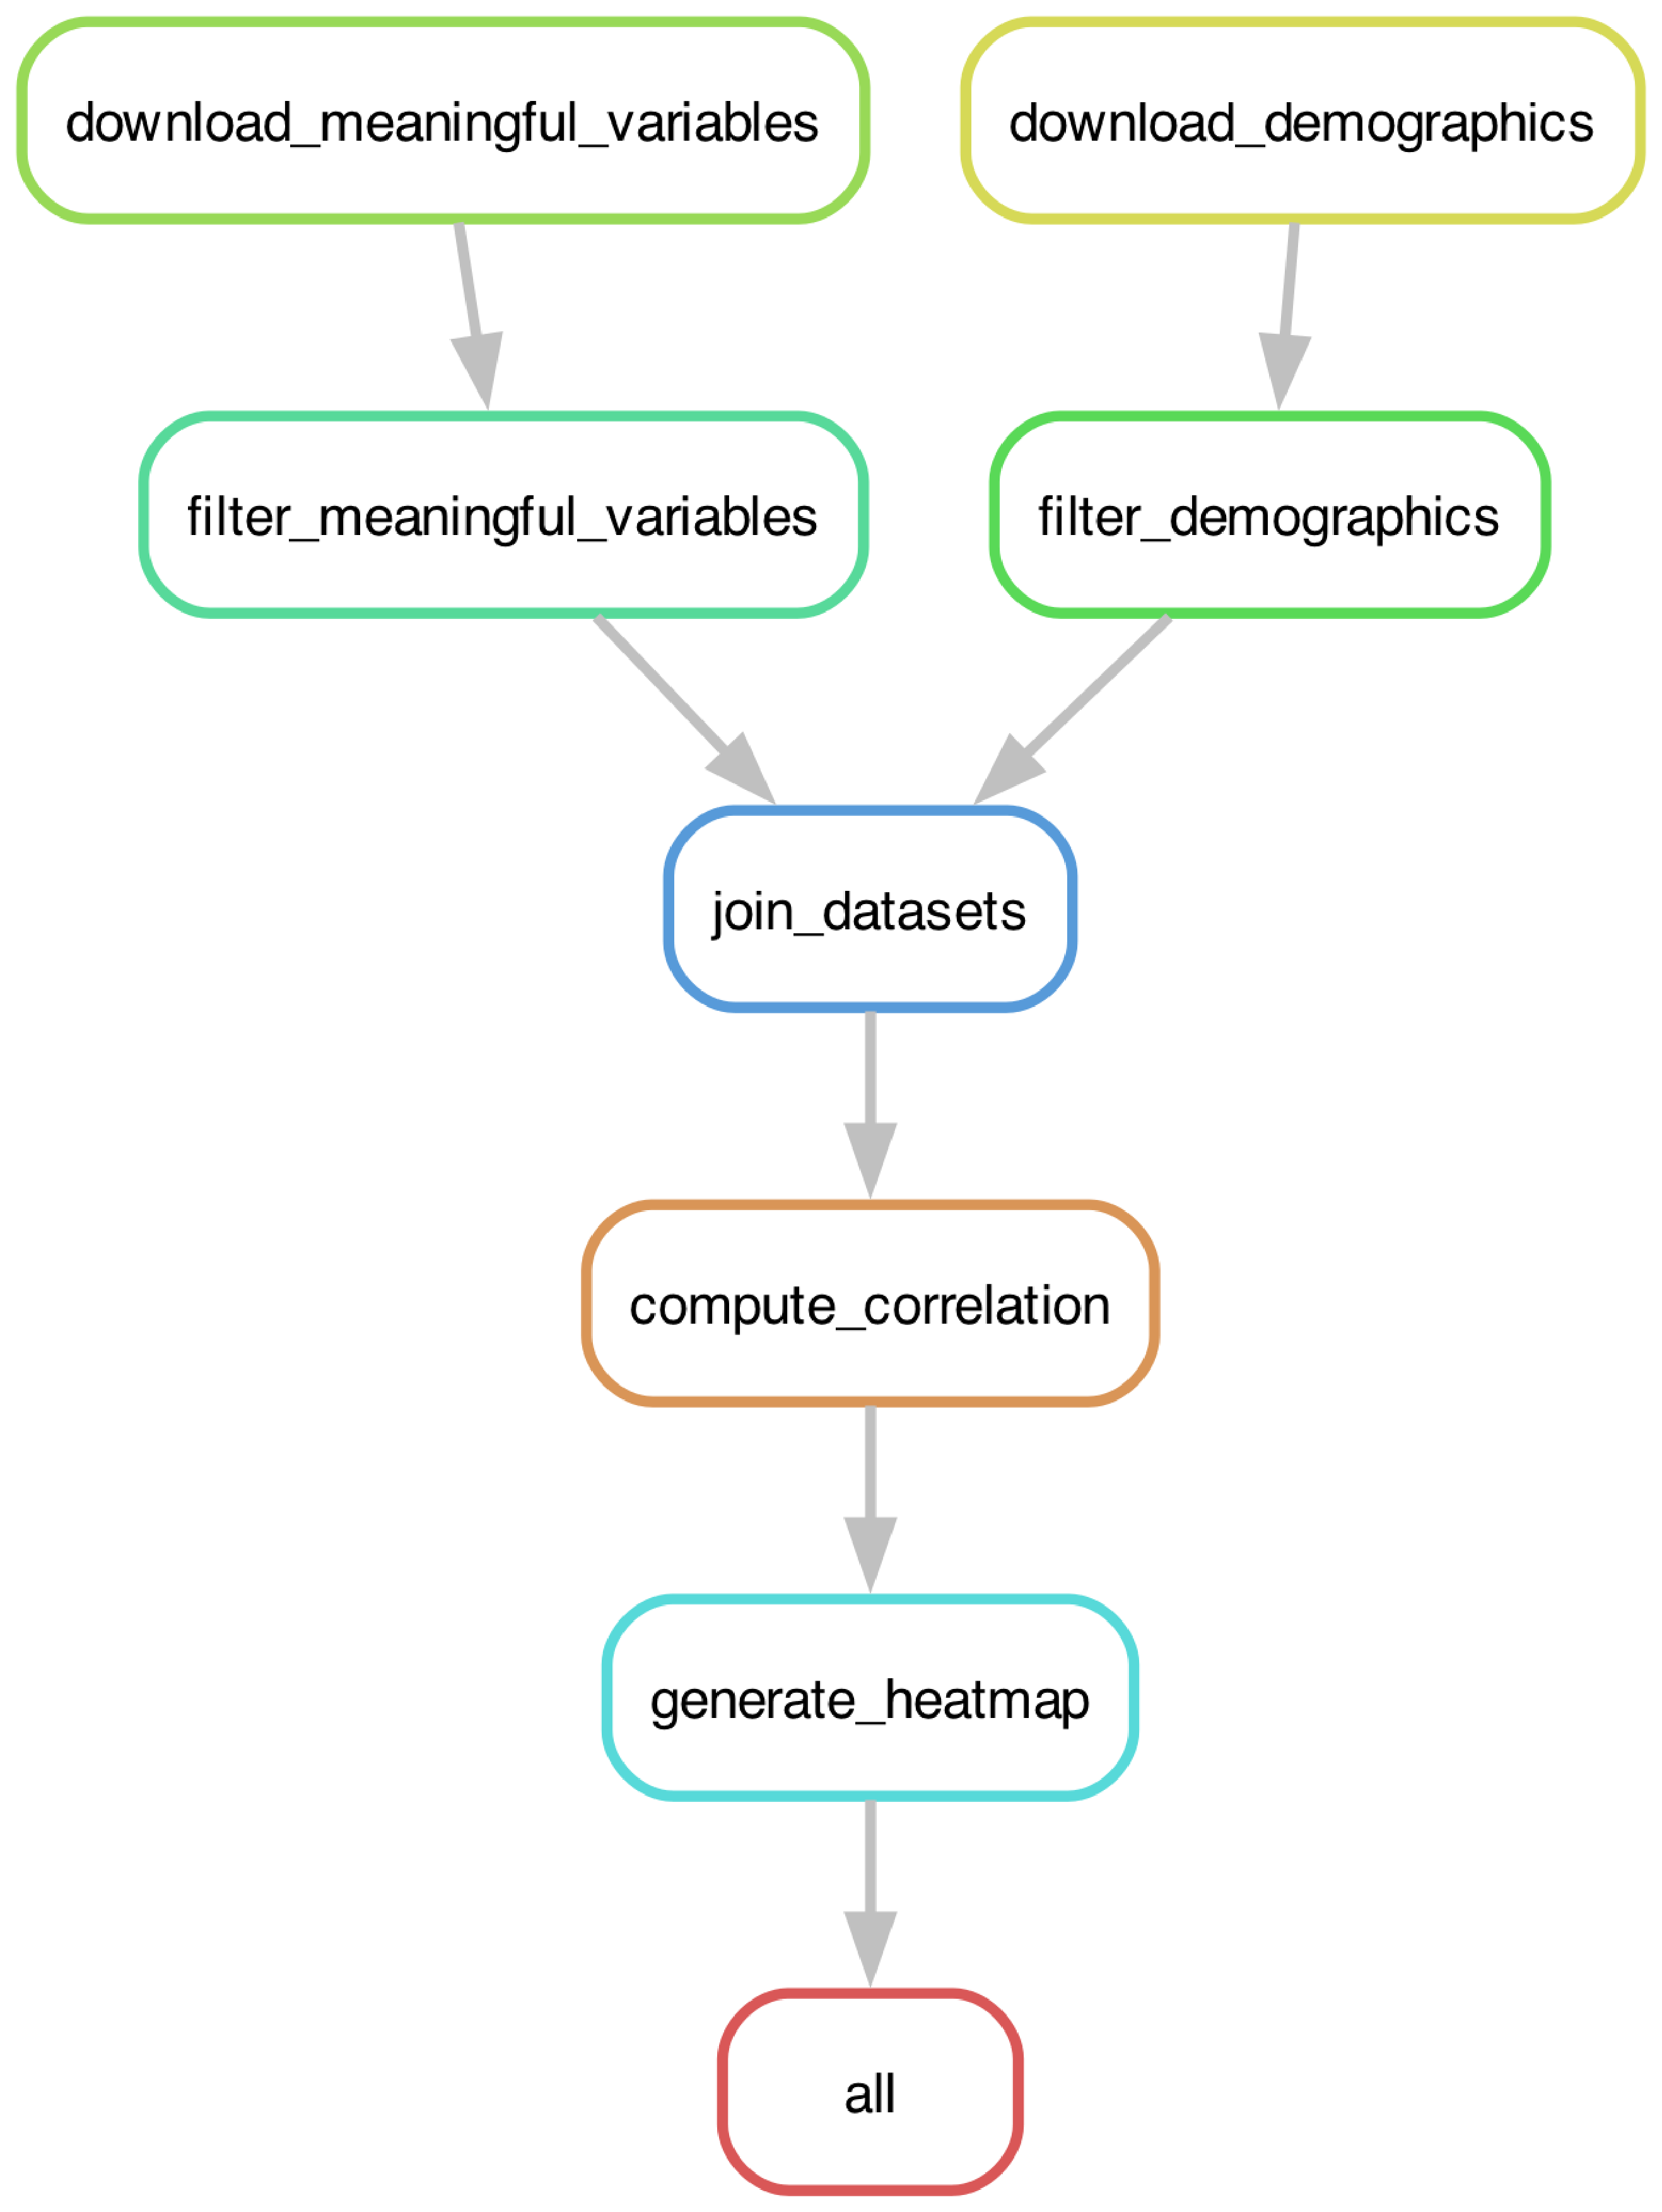
\includegraphics[width=0.375\linewidth]{figures/08/simpleDAG.pdf}
\caption[Execution graph for simple example]{The execution graph for the simple example analysis workflow visualized as a DAG.}
\label{simpleDAG-fig}
\end{figure}

The use of DAGs to represent workflows provides a number of important benefits:

\begin{itemize}
\item The engine can identify independent pathways through the graph, which can then be executed in parallel
\item If one node of the graph changes, the engine can identify which downstream nodes need to be rerun
\item If a node fails, the engine can be configured to continue with executing the nodes that don't depend on the failed node either directly or indirectly
\end{itemize}

There are a couple of additional benefits to using a workflow engine, which I will discuss in more detail in the context of a more complex workflow. The first is that they generally deal automatically with the storage of intermediate results (known as \textit{caching} or \textit{checkpointing}), which can help speed up execution when nothing has changed and allow continued execution if the process is interrupted.  The second is that the workflow engine uses the execution graph to optimize the schedule of computations, only performing those operations that are actually needed.  This is similar in spirit to the concept of \textit{lazy execution} used by packages like \textit{Polars}, in which the system optimizes computational efficiency by first analyzing the full computational graph.\index{Polars}\index{caching}

\subsection{General-purpose versus domain-specific workflow engines}

With the growth of data science within industry and research, there has been an explosion of new workflow management systems that aim to solve particular problems; a list of these can be found at \href{https://github.com/meirwah/awesome-workflow-engines}{awesome-workflow-engines}. It's also worth noting that there are a number of domain-specific workflow engines that are specialized for particular kinds of data and workflows.  Examples include \href{https://galaxyproject.org/}{\textit{Galaxy}} which is specialized for bioinformatics and genomics, and \href{https://nipype.readthedocs.io/en/latest/index.html}{\textit{Nipype}} which is specialized for neuroimaging analysis workflows. If your research community uses one of these then it's worth exploring that engine as your first option, since it will probably be well supported within the community. However, a benefit of using a general-purpose engine is that they will often be better maintained and supported, and AI tools will likely have more examples to work from when generating new workflows.\index{Galaxy}\index{Nipype}

\section{Workflow management using Snakemake}

I will use the \href{https://snakemake.readthedocs.io/en/stable/}{\textit{Snakemake}} workflow system for this example, which I chose for several reasons:

\begin{itemize}
\item It is a very well-established project that is actively maintained.
\item It is Python-based, which makes it easy for Python users to grasp.
\item Because of its long history and wide use, AI coding assistants are quite familiar with it and can easily generate the necessary files for complex workflows.
\end{itemize}

\textit{Snakemake} is a sort of ``make on steroids'', designed specifically to manage complex computational workflows.  It uses a Python-like syntax to define the workflow, from which it infers the computational graph and optimizes the computation. The \textit{Snakemake} workflow is defined using a \texttt{Snakefile}, the most important aspect of which is a set of rules that define the different workflow steps in terms of their outputs.  Here is an initial portion of the \texttt{Snakefile} for our simple workflow:

\begin{lstlisting}[style=Python]
# Base directory (where `Snakefile`  is located)
BASEDIR = workflow.basedir

# Output directories (relative to working directory set via -d)
DATA_DIR = "data"
RESULTS_DIR = "results"
FIGURES_DIR = "figures"
LOGS_DIR = "logs"

# Load configuration
configfile: f"{BASEDIR}/config/config.yaml"

# Global report
report: f"{BASEDIR}/report/workflow.rst"

# Default target
rule all:
    input:
        f"{FIGURES_DIR}/correlation_heatmap.png",
\end{lstlisting}

What this does is first specify a set of directories; the \texttt{BASEDIR} variable refers to the directory where the \texttt{Snakefile}  is found, while the other directories are specified with the respect to the working directory that is specified using the \texttt{-d} argument.  It then specifies the location of the configuration file, which is a YAML file that defines various parameters for the workflow.  Here are the contents of the config file for our simple example:\index{YAML}

\begin{lstlisting}[style=yaml]
# Data URLs
meaningful_variables_url: "<URL deleted for brevity>"
demographics_url: "<URL deleted for brevity>"

# Correlation settings
correlation_method: "spearman"

# Heatmap settings
heatmap:
  figsize: [12, 10]
  cmap: "coolwarm"
  vmin:-1.0
  vmax: 1.0
\end{lstlisting}

The only rule shown above is the \texttt{all} rule, which takes as its input the correlation figure that is the final output of the workflow.  If snakemake is called and that file already exists, then it won't be rerun (since it's the only requirement for the rule) unless 1) the \texttt{--force} flag is included, which forces rerunning the entire workflow, or 2) a rerun is triggered by one of the changes to the input files, parameters, or the code itself.  If the file doesn't exist, then \textit{Snakemake} examines the additional rules to determine which steps need to be run in order to generate that output.  In this case, it would start with the rule that generates the correlation figure:

\begin{lstlisting}[style=Python]
# Step 5: Generate clustered heatmap
rule generate_heatmap:
    input:
        f"{RESULTS_DIR}/correlation_matrix.csv",
    output:
        report(
            f"{FIGURES_DIR}/correlation_heatmap.png",
            caption=f"{BASEDIR}/report/heatmap.rst",
            category="Results",
        ),
    params:
        figsize=config["heatmap"]["figsize"],
        cmap=config["heatmap"]["cmap"],
        vmin=config["heatmap"]["vmin"],
        vmax=config["heatmap"]["vmax"],
    log:
        f"{LOGS_DIR}/generate_heatmap.log",
    conda:
        f"{BASEDIR}/envs/simple.yml"
    script:
        f"{BASEDIR}/scripts/generate_heatmap.py"
\end{lstlisting}

This step uses the \texttt{generate\_heatmap.py} script to generate the correlation figure, and it requires the \texttt{correlation\_matrix.csv} file as input.  Note that while there is a \textit{Conda} directive in this rule, which we will discuss further below, \textit{Conda} is not actually used unless the \texttt{--use-conda} flag is provided.  \textit{Snakemake} would then work backward to identify which step is required to generate that file, which is the following:\index{Conda}

\begin{lstlisting}[style=Python]
# Step 4: Compute correlation matrix
rule compute_correlation:
    input:
        f"{DATA_DIR}/joined_data.csv",
    output:
        f"{RESULTS_DIR}/correlation_matrix.csv",
    params:
        method=config["correlation_method"],
    log:
        f"{LOGS_DIR}/compute_correlation.log",
    conda:
        f"{BASEDIR}/envs/simple.yml"
    script:
        f"{BASEDIR}/scripts/compute_correlation.py"
\end{lstlisting}

By working backwards this way from the intended output, \textit{Snakemake} can reconstruct the computational graph that we saw in Figure~\ref{simpleDAG-fig}.  It then uses this graph to plan the computations that will be performed.

\subsection{\textit{Snakemake} scripts}

In order for \textit{Snakemake} to execute each of our modules, we need to wrap those modules in a script that can use the configuration information from the config file.  Here is an example of what the \href{https://github.com/BetterCodeBetterScience/example-simpleworkflow/blob/main/snakemake\_workflow/scripts/generate\_heatmap.py}{generate\_heatmap.py} script would look like:

\begin{lstlisting}[style=Python]
from pathlib import Path
import pandas as pd
from bettercode.simple_workflow.visualization import (
    generate_clustered_heatmap,
)

def main() -> None:
    """Generate and save clustered heatmap."""
    # ruff: noqa: F821
    input_path = Path(snakemake.input[0])
    output_path = Path(snakemake.output[0])
    figsize = tuple(snakemake.params.figsize)
    cmap = snakemake.params.cmap
    vmin = snakemake.params.vmin
    vmax = snakemake.params.vmax

    # Load correlation matrix
    corr_matrix = pd.read_csv(input_path, index_col=0)
    print(f"Loaded correlation matrix: {corr_matrix.shape}")

    # Generate heatmap
    generate_clustered_heatmap(
        corr_matrix,
        output_path=output_path,
        figsize=figsize,
        cmap=cmap,
        vmin=vmin,
        vmax=vmax,
    )
    print(f"Saved heatmap to {output_path}")

if __name__ == "__main__":
    main()
\end{lstlisting}

You can see that the code refers to the \texttt{snakemake} module even though we haven't explicitly imported it; this is possible because the script is executed within the \textit{Snakemake} environment which makes the \texttt{snakemake} object available within the script's execution namespace, containing all of the configuration details.  

Once the \texttt{Snakefile}  and other related files are ready to go, we can first check whether they are properly formatted using \texttt{snakemake --lint}, which is a static analysis tool specifically for snakemake configuration files.  Here is the result (note: some output lines are omitted for conciseness):\index{static analysis}

\begin{lstlisting}[style=shell, numbers=none]
$ uv run snakemake --lint --cores 1 -d ./output

Congratulations, your workflow is in a good condition!
\end{lstlisting}

We are now ready to run the \texttt{snakemake} command, which will need to include several configuration directives. Let's first do a ``dry run'' which creates the execution graph but doesn't actually execute anything:

\begin{lstlisting}[style=shell]
$ uv run snakemake --dry-run --cores 1 -d ./output

Building DAG of jobs...

Job stats:
job                              count
--------------------------------------
all                                  1
compute_correlation                  1
download_demographics                1
download_meaningful_variables        1
filter_demographics                  1
filter_meaningful_variables          1
generate_heatmap                     1
join_datasets                        1
total                                8

... (omitting intermediate output)

Job stats:
job                              count
--------------------------------------
all                                  1
compute_correlation                  1
download_demographics                1
download_meaningful_variables        1
filter_demographics                  1
filter_meaningful_variables          1
generate_heatmap                     1
join_datasets                        1
total                                8

Reasons:
    (check individual jobs above for details)
    input files updated by another job:
        all, compute_correlation, filter_demographics, filter_meaningful_variables, generate_heatmap, join_datasets
    output files have to be generated:
        compute_correlation, download_demographics, download_meaningful_variables, filter_demographics, filter_meaningful_variables, generate_heatmap, join_datasets
This was a dry-run (flag -n). The order of jobs does not reflect the order of execution.
\end{lstlisting}

Once we have confirmed that everything is set up properly, we can then use \texttt{snakemake} to run the workflow:

\begin{lstlisting}[style=shell]
$ uv run snakemake --cores 1 -d ./output

Building DAG of jobs...

Job stats:
job                              count
--------------------------------------
all                                  1
compute_correlation                  1
download_demographics                1
download_meaningful_variables        1
filter_demographics                  1
filter_meaningful_variables          1
generate_heatmap                     1
join_datasets                        1
total                                8

Select jobs to execute...
Execute 1 jobs...

[Wed Dec 24 08:17:57 2025]
localrule download_demographics:
    output: output/data/demographics.csv
    log: output/logs/download_demographics.log
    jobid: 7
    reason: Missing output files: output/data/demographics.csv
    resources: tmpdir=/var/folders/r2/f85nyfr1785fj4257wkdj7480000gn/T
Downloaded 522 rows from <URL deleted for brevity>
Saved to output/data/demographics.csv
[Wed Dec 24 08:17:58 2025]
Finished jobid: 7 (Rule: download_demographics)
1 of 8 steps (12%) done

... (omitting intermediate output)

8 of 8 steps (100%) done
Complete log(s): .snakemake/log/2025-12-24T081757.266320.snakemake.log
\end{lstlisting}

It's important to know that when \textit{Snakemake} is run, it stores metadata regarding the workflow in a hidden directory called \texttt{.snakemake}, including the log file mentioned at the end of the output above. This directory can carry over hidden state from previous runs that can become confusing when debugging. It's sometimes useful to remove this directory as a last resort (when the \texttt{--force } and \texttt{--cleanup-metadata} are not sufficient).\index{debugging}

One handy feature of \textit{Snakemake} is that, just like \textit{make}, we can give it a specific target file and it will perform only the portions of the workflow that are required to regenerate that specific file. For example, let's say that the file \texttt{output/data/demographics.csv} became corrupted and you needed to recreate it.  This could be done using the command:

\begin{lstlisting}[style=shell, numbers=none]
$ uv run snakemake output/data/demographics.csv --cores 1 -d ./output
\end{lstlisting}

\subsection{Updating the workflow when inputs change}

Once the workflow has completed successfully, re-running it will not result in the re-execution of any of the analyses:

\begin{lstlisting}[style=shellshort]
$ uv run snakemake --cores 1 -d ./output

Building DAG of jobs...
Nothing to be done (all requested files are present and up to date).
\end{lstlisting}

However, \textit{Snakemake} checks several features of the workflow (by default) when generating its DAG to see if anything relevant has changed.  By default it checks to see if any of the following have changed (configurable using the \texttt{-rerun-triggers} flag):

\begin{itemize}
\item modification times of input files
\item the code specified within the rule
\item the input files or parameters for the rule
\end{itemize}

Snakemake also checks for changes in the details of the software environment, but as of the date of writing this only works for \textit{Conda} environments.

As an example, I will first update the modification time of the meaningful variables file from a previous successful run using the \texttt{touch} command:

\begin{lstlisting}[style=shell]
$  ls -l ./output/data/meaningful_variables.csv
Permissions Size User     Date Modified Name
.rw-r--r--@ 1.2M poldrack 24 Dec 10:11  data/meaningful_variables.csv

$  touch ./output/data/meaningful_variables.csv

$  ls -l ./output/data/meaningful_variables.csv
Permissions Size User     Date Modified Name
.rw-r--r--@ 1.2M poldrack 24 Dec 10:14  data/meaningful_variables.csv
\end{lstlisting}

You can see that the touch command updated the modification time of the file.  Now let's rerun the \texttt{snakemake} command:

\begin{lstlisting}[style=shell]
$ uv run snakemake --cores 1 -d ./output

Building DAG of jobs...

Job stats:
job                            count
--------------------------------------
all                                1
compute_correlation                1
filter_meaningful_variables        1
generate_heatmap                   1
join_datasets                      1
total                              5
\end{lstlisting}

Similarly, \textit{Snakemake} will rerun the workflow if any of the scripts used to run the workflow are modified.  However, it's important to note that it will not identify changes in the modules that are imported.  In that case you would need to rerun the workflow using the \texttt{--force} flag in order to re-execute the relevant steps.

\subsection{Reproducible environments with Conda}

\textit{Snakemake} comes with native support for \textit{Conda} environments, which helps ensure reproducibility across systems. As I discussed in Chapter 2, I generally prefer \textit{uv} over  \textit{Conda}, but \textit{Snakemake} does not support  \textit{uv} environments at the time of writing, so \textit{Conda} is the only option until that support becomes available.  After first installing \textit{Conda} on our system (if necessary), we then need to identify all of the packages that are necessary for our workflow to succeed, and then add those to a YAML file. Here is the example for our simple workflow, which I placed in \texttt{envs/simple.yaml}:\index{reproducibility}

\begin{lstlisting}[style=yaml]
name: bettercode
channels:
 - conda-forge
dependencies:
 - numpy=2.4.0
 - pandas=2.3.3
 - matplotlib=3.10.8
 - seaborn=0.13.2
\end{lstlisting}

When we run the workflow, we will see that \textit{Snakemake} first builds a local \textit{Conda} environment within the working directory. In this case I am running it from a different directory than the source directory, so I need to specify the location of the \texttt{Snakefile}:

\begin{lstlisting}[style=shell]
$ uv run snakemake --sdm conda --snakefile /path/to/Snakefile -d ./ --cores 15

Building DAG of jobs...
Creating *Conda* environment /path/to/snakemake_workflow/envs/simple.yml...
Downloading and installing remote packages.
Cleaning up *Conda* package tarballs.
Environment for /path/to/snakemake_workflow/envs/simple.yml created (location: .snakemake/conda/0f65d58d0ced6388a583c7e1b77c240e_)
\end{lstlisting}

It then uses this environment to execute the code.  It's worth nothing that this will leave the \textit{Conda} environment in place within the hidden \texttt{.snakemake} directory, which can take up a significant amount of disk space if there are a lot of dependencies.

\subsection{Reproducible environments with containers}

As I discussed in Chapter 6, software containers are increasingly used as a means for creating reproducible software environments. \textit{Snakemake} has built-in support for the \textit{Apptainer} container tool, which is available for Linux and installed on most high-performance computing systems, but unfortunately not easily usable on Mac or Windows systems. Here I will show an example of a containerized version of the simple workflow above, running on my local Linux system.\index{Apptainer}\index{high-performance computing}

Using containers is easiest if you can find an existing Docker container that contains all of the necessary dependencies for your code.  Fortunately there is a large number of containers available via the \href{https://hub.docker.com/}{Docker Hub}, and given the simple dependencies that our workflow requires, I was easily able to find \href{https://hub.docker.com/layers/jupyter/scipy-notebook/x86\_64-ubuntu-22.04/images/sha256-3b37958b7b31ce94c3027d7c83c98fc16acfe166fab2de2f62ae54c50e59aed3}{a container} containing the necessary packages.  I added this to my \texttt{config.yaml} file:\index{SciPy}\index{Docker}\index{Docker Hub}

\begin{lstlisting}[style=yaml]
# Container image (used with --sdm apptainer)
container: "docker://jupyter/scipy-notebook:x86_64-ubuntu-22.04"
\end{lstlisting}

and also added the definition to my \texttt{Snakemake} file:

\begin{lstlisting}[style=Python]
# Container image for all rules (used with --sdm apptainer)
container: config["container"]
\end{lstlisting}

and then ran the \textit{Snakemake} command specifying apptainer as my dependency management system:\index{dependency management}

\begin{lstlisting}[style=shell]
$ uv run snakemake --cores 1 --sdm apptainer -d ./output

Building DAG of jobs...
Pulling singularity image docker://jupyter/scipy-notebook:x86_64-ubuntu-22.04.
...
\end{lstlisting}

As with \textit{Conda}, it's worth noting that \textit{Snakemake} will store the \textit{Apptainer} image within the \texttt{.snakemake} directory, which can sometimes be quite large; for the \textit{Jupyter} image linked above, it was about 1.2 GB, but I have seen containers up to 10 GB or more on occasion.\index{Jupyter}

\subsection{Best practices for \textit{Snakemake} workflows}

The \textit{Snakemake} team has published a set of \href{https://snakemake.readthedocs.io/en/stable/snakefiles/best\_practices.html}{best practices} for the creation of \textit{Snakemake} workflows, some of which I will outline here, along with one of my own (the first).

\subsubsection{Using a working directory}

By default \textit{Snakemake} looks for a \texttt{Snakefile} in the current directory, so it's tempting to run the workflow from the code repository.  However, \textit{Snakemake} creates a directory called \texttt{.snakemake} to store metadata in the directory where the workflow is run, which one generally doesn't want to mix with the code.  Thus, it's best to run the command using the \texttt{--snakefile} directive to point to the \texttt{Snakefile} located in the code directory, and setting the working directory to the intended output directory using the \texttt{-d} flag. This will fail if you run the command from a location other than the source folder if the paths in the snakemake rules are specified using relative paths, like this:

\begin{lstlisting}[style=Pythonshort]
script:
        f"scripts/aggregate_results.py"
\end{lstlisting}

This happens because relative paths inside the \texttt{Snakefile} are interpreted as relative to the working directory, not the directory where the \texttt{Snakefile} is located.  Instead, we need to use the \texttt{workflow.basedir} prefix, which refers to the directory where the \texttt{Snakefile} is located:

\begin{lstlisting}[style=Pythonshort]
script:
        f"{workflow.basedir}/scripts/aggregate_results.py"
\end{lstlisting}

\subsubsection{Workflow organization}

There is a \href{https://snakemake.readthedocs.io/en/stable/snakefiles/deployment.html\#distribution-and-reproducibility}{standard format} for the organization of \textit{Snakemake} workflow directories, which one should follow when developing new workflows.

\subsubsection{\texttt{Snakefile} formatting}

\textit{Snakemake} comes with a set of commands that help ensure that configuration files are properly formatted and follow best practices.  As I mentioned above, there is a static analysis tool (i.e., a ``linter'', akin to \textit{ruff} or \textit{flake8} for Python code), which can automatically identify syntax errors and logical problems with \textit{Snakemake} rule files.  Users of \textit{uv} should note that the \textit{Snakemake} linter assumes that one is using the \textit{Conda} environment manager or a container, and it raises an issue for any rule that doesn't specify a \textit{Conda} or container environment. Nonetheless, if those are ignored the linter can be useful in identifying problems. There is also a formatting tool called \texttt{snakefmt} (separately installed) that optimally formats \textit{Snakemake} files in the way that \textit{black} or \textit{ruff} format Python code.  These can both be useful tools when developing a new workflow.\index{flake8}\index{ruff}

\subsubsection{Configurability}

Workflow configuration details should be stored in configuration files, such as the \texttt{config.yaml} files that we have used in our workflow examples.  However, these files should not be used for runtime parameters, such as the number of cores or the output directory; those should instead be handled using Snakemake's standard arguments.

\subsection{Report generation}

One of the very handy features of \textit{Snakemake} is its ability to generate reports for workflow execution.  Report generation is as simple as:

\begin{lstlisting}[style=shell, numbers=none]
$ uv run snakemake -c 1 --report output/report.html -d output
\end{lstlisting}

This command uses the metadata stored in the \texttt{.snakemake} directory along with details provided in separate report formatting files that are located within the \texttt{report} directory alongside the \texttt{Snakefile}. In order for an output (such as a figure) to be included in the report, it needs to be marked with a \texttt{report} flag in the output section of the relevant rule.  For example, to have a correlation heatmap added to the report, I used the following statement:

\begin{lstlisting}[style=Python]
rule generate_heatmap:
    input:
        f"{RESULTS_DIR}/correlation_matrix.csv",
    output:
        report(
            f"{FIGURES_DIR}/correlation_heatmap.png",
            caption=f"{BASEDIR}/report/heatmap.rst",
            category="Results",
        ),
\end{lstlisting}

Running the report generation command generates a single self-contained HTML file, with any figures embedded within the file, making them very handy for sharing.

\subsection{Tracking provenance}

As I discussed in the earlier chapter on data management, it is essential to be able to track the provenance of files in a workflow.  That is, how did the file come to be, and what other files did it depend on?  \textit{Snakemake} stores a substantial amount of metadata that allows us to reconstruct much of the provenance of any file generated by a workflow.  The relevant data are stored within the \texttt{.snakemake/metadata} directory, which on first glance seems to contain a bunch of gibberish:

\begin{lstlisting}[style=shell]
$  ls .snakemake/metadata

cmVzdWx0cy9jb3JyZWxhdGlvbl9tYXRyaXguY3N2
ZGF0YS9kZW1vZ3JhcGhpY3MuY3N2
ZGF0YS9kZW1vZ3JhcGhpY3NfbnVtZXJpY2FsLmNzdg==
ZGF0YS9qb2luZWRfZGF0YS5jc3Y=
ZGF0YS9tZWFuaW5nZnVsX3ZhcmlhYmxlc19udW1lcmljYWwuY3N2
ZGF0YS9tZWFuaW5nZnVsX3ZhcmlhYmxlcy5jc3Y=
ZmlndXJlcy9jb3JyZWxhdGlvbl9oZWF0bWFwLnBuZw==
\end{lstlisting}

These filenames are actually versions of the original filenames that have been encoded into a \textit{base64} representation that makes them easily saveable as a single file.  We can decode them using the \texttt{base64} python package:

\begin{lstlisting}[style=repl]
In : encoded_name
Out: 'ZGF0YS9tZWFuaW5nZnVsX3ZhcmlhYmxlc19udW1lcmljYWwuY3N2'

In : import base64

In : base64.b64decode(encoded_name).decode()
Out: 'data/meaningful_variables_numerical.csv'
\end{lstlisting}

These files are stored in JSON format and contain a dictionary with relevant information about the provenance of each file:\index{JSON}

\begin{lstlisting}[style=Pythonshort]
metadata_path = f".snakemake/metadata/{encoded_name}"
with open(metadata_path) as f:
    print(md_dict)
\end{lstlisting}

\begin{lstlisting}[style=json]
{'record_format_version': 6,
 'code': '        f"{BASEDIR}/scripts/filter_data.py"\n',
 'rule': 'filter_meaningful_variables',
 'input': ['data/meaningful_variables.csv'],
 'log': ['logs/filter_meaningful_variables.log'],
 'params': [],
 'shellcmd': None,
 'incomplete': False,
 'starttime': 1767284094.3992934,
 'endtime': 1767284095.986599,
 'job_hash': 278889477,
 'conda_env': 'bmFtZTogc2ltcGxlX3dvcmtmbG93CmNoYW5uZWxzOgogIC',
 'software_stack_hash': 'd41d8cd98f00b204e9800998ecf8427e',
 'container_img_url': 'docker://jupyter/scipy-notebook:x86_64-ubuntu-22.04',
 'input_checksums': {}}
\end{lstlisting}

Using this information we could reconstruct the DAG for the workflow, or identify the specific files that went into generating each other file.

\subsubsection{Generating a PROV representation from Snakemake}

As I mentioned in the chapter on data management, there is a emerging standard for representation of provenance information, known as \textit{PROV}.  Although \textit{Snakemake} does not directly support the generation of \textit{PROV} representations, there is a package called \href{https://pypi.org/project/makeprov/}{\textit{makeprov}} that can generate a \textit{PROV} representation from a \textit{Snakemake} workflow.  After running our workflow and installing the \textit{makeprov} package, we simply need to run the \texttt{snakemake.makeprov} command to generate the PROV output from within the working directory of the workflow (where the .snakemake directory is located):

\begin{lstlisting}[style=shell, numbers=none]
$ uv run python -m makeprov.snakemake --prov -path prov/snakemake -- --snakefile path/to/Snakefile --nolock
\end{lstlisting}

This will generate a file called \texttt{prov/snakemake.json} that contains representations of each of the entities and activities in the workflow.  For example, the representation of the \texttt{data/meaningful\_variables\_numerical.csv} output file would look like this:

\begin{lstlisting}[style=json]
{
      "id": "urn:snakemake:file/data/meaningful_variables_numerical.csv",
      "type": "prov:Entity",
      "format": "text/csv",
      "extent": 1191564,
      "modified": "2026-01-01T16:14:55.986599+00:00",
      "identifier": "sha256:6e09083ea4f474b420cf1ca9f42486e4a509ad020a39f5432b4c183e7f92e519",
      "wasGeneratedBy": "urn:snakemake:job/4",
      "label": "data/meaningful_variables_numerical.csv"
    },
\end{lstlisting}

and the representation of the job that created it (\texttt{filter\_meaningful\_variables}) would look like this:

\begin{lstlisting}[style=json]
{
      "id": "urn:snakemake:job/4",
      "type": "prov:Activity",
      "wasAssociatedWith": "urn:snakemake:agent/snakemake",
      "used": [
        "urn:snakemake:file/data/meaningful_variables.csv"
      ],
      "label": "filter_meaningful_variables (jobid=4)",
      "snakemake:rule": "filter_meaningful_variables",
      "snakemake:status": "ok",
      "snakemake:plan": "no update"
    },
\end{lstlisting}

These files provide a very useful representation of the provenance for a workflow, and demonstrate the power of using a workflow engine that stores rich metadata about the workflow and its execution.

\section{Scaling to a complex workflow}

We now turn to a more realistic and complex scientific data analysis workflow. For this example I will use an analysis of single-cell RNA-sequencing data to determine how gene expression in immune system cells changes with age. This analysis will utilize a \href{https://cellxgene.cziscience.com/collections/dde06e0f-ab3b-46be-96a2-a8082383c4a1}{large openly available dataset} that includes data from 982 people comprising about 1.3 million peripheral blood mononuclear cells (i.e. white blood cells) for about 35K transcripts.  I chose this particular example for several reasons:

\begin{itemize}
\item It is a realistic example of a workflow that a researcher might actually perform.
\item It has a large enough sample size to provide a robust answer to our scientific question.
\item The data are large enough to call for a real workflow management scheme, but small enough to be processed on a single laptop (assuming it has decent memory).
\item The workflow has many different steps, some of which can take a significant amount of time (over one hour)
\item There is an established Python library (\href{https://scanpy.readthedocs.io/en/stable/}{\textit{scanpy}}) that implements the necessary workflow components.
\item It's an example outside of my own research domain, to help demonstrate the applicability of the book's ideas across a broader set of data types.
\end{itemize}

I will use this example to show how to move from a monolithic analysis script to a well-structured and usable workflow that meets most of the desired features described above.

\section{Starting point: One huge notebook}

I developed the initial version of this workflow as many researchers would: by creating a \textit{Jupyter} notebook that implements the entire workflow, which can be found \href{https://github.com/BetterCodeBetterScience/example-rnaseq/blob/main/notebooks/immune\_scrnaseq\_2\_preprocess.ipynb}{here}. The total execution time for this notebook is about two hours on an M3 Max Macbook Pro.

\subsection{The problem of in-place operations}

What I found as I developed the workflow was that I increasingly ran into problems that arose because the state of particular objects had changed.  This occurred for two reasons at different points.  In some cases it occurred because I saved a new version of the object to the same name, resulting in an object with different structure than before.  Second, and more insidiously, it occurred when an object passed into a function was modified by the function internally.  This is known as an \textit{in-place} operation, in which a function modifies an object directly rather than returning a new object that can be assigned to a variable.

In-place operations can make code particularly difficult to debug in the context of a \textit{Jupyter} notebook, because it's a case where out-of-order execution can result in very confusing results or errors, since the changes that were made in-place may not be obvious.  For this reason, I generally avoid any kind of in-place operations if possible.  Rather, any function should immediately create a copy of the object that was passed in, and then do its work on that copy, returning at the end of the function for assignment to a new variable.  One can then re-assign it to the same variable name if desired, which is more transparent than an in-place operation but still makes the workflow dependent on the exact state of execution and can lead to confusion when debugging.  Some packages allow a feature called ``copy-on-write'' which defers actually copying the data in memory until it is actually modified, which can make copying more efficient; this feature is becoming the default in \textit{pandas}.

If one must modify objects in-place, then it is good practice to announce this loudly.  The loudest way to do this would be to put ``inplace'' in the function name. Another cleaner but less loud way is through conventions regarding function naming; for example, in \textit{PyTorch} it is a convention that any function that ends with an underscore (e.g. \texttt{tensor.mul\_(x)}) performs an in-place operation whereas the same function without the underscore (\texttt{tensor.mul(x)}) returns a new object. Another way that some packages enable explicit in-place operations is through a function argument (e.g. \texttt{inplace=True} in \textit{pandas}), though this is being phased out from many functions in \textit{pandas} because ``It is generally seen (at least by several \textit{pandas} maintainers and educators) as bad practice and often unnecessary'' (\href{https://pandas.pydata.org/pdeps/0008-inplace-methods-in-pandas.html}{PDEP-8}).\index{PyTorch}

One way to prevent in-place operations altogether is to use data types that are \textit{immutable}, meaning that they can't be changed once created.  This is one of the central principles in \textit{functional programming} languages (such as Haskell), where all data types are immutable, such that one is required to create a new object any time data are modified.  Some native data types in Python are immutable (such as tuples and frozensets), and some data science packages also provide immutable data types; in particular, the \textit{Polars} package (which is meant to be a high-performance alternative to pandas) implements its version of a data frame as an immutable object, and the \textit{JAX} package (for high-performance numerical computation and machine learning) implements immutable numerical arrays.\index{JAX}\index{machine learning}\index{functional programming}

\subsection{Converting from \textit{Jupyter} notebook to a runnable python script}

As we discussed in an earlier chapter, converting a \textit{Jupyter} notebook to a pure Python script is easy using \textit{jupytext}.  This results in a script that can be run from the command line.  However, there can be some commands that will block execution of the script; in particular, plotting commands can open windows that will block execution until they are closed.  To prevent this, and to ensure that the results of the plots are saved for later examination, I replaced all of the \texttt{plt.show()} commands that display a figure to the screen with \texttt{plt.savefig()} commands that save the figures to a file in the results directory.  (This was an easy job for the my AI coding agent to complete.)

\section{Decomposing a complex workflow}

The first thing we need to do with a large monolithic workflow is to determine how to decompose it into coherent modules.  There are various reasons that one might choose a particular breakpoint between modules.  First and foremost, there are usually different stages that do conceptually different things.  In our example, we can break the workflow into several high-level processes:\index{breakpoint}

\begin{itemize}
\item Data (down)loading
\item Data filtering (removing subjects or cell types with insufficient observations)
\item Quality control

\begin{itemize}
\item identifying bad cells on the basis of mitochondrial, ribosomal, or hemoglobin genes or hemoglobin contamination
\item identifying ``doublets'' (two cells captured in a single barcode)
\end{itemize}

\item Preprocessing

\begin{itemize}
\item Count normalization
\item Log transformation
\item Identification of high-variance features
\item Filtering of nuisance genes
\end{itemize}

\item Dimensionality reduction
\item UMAP generation
\item Clustering
\item Pseudobulking (aggregating cells within an individual)
\item Differential expression analysis
\item Pathway enrichment analysis (GSEA)
\item Overrepresentation analysis (Enrichr)
\item Predictive modeling
\end{itemize}

In addition to a conceptual breakdown, there are also other reasons that one might want to further decompose the workflow:

\begin{itemize}
\item There may be points where one might need to restart the computation (e.g. due to computational cost).
\item There may be sections where one might wish to swap in a new method or different parameterization.
\item There may be points where the output could be reusable elsewhere.
\end{itemize}

\section{Resumable workflows}

I asked my coding agent to help modularize the monolithic workflow, using a prompt that provided the conceptual breakdown described above.  The resulting code ran correctly, but crashed about two hours into the process due to a resource issue that appeared to be due to asking for too many CPU cores in the differential expression analysis.  This left me in the situation of having to rerun the entire two hours of preliminary workflow simply to get to a point where I could test my fix for the differential expression component, which is not a particularly efficient way of coding.  The problem here is that the workflow execution was \textit{stateful}, in the sense that the previous steps need to be rerun prior to performing the current step in order to establish the required objects in memory.  The solution to this problem is to implement the workflow in a \textit{resumable} way, which doesn't require that earlier steps be rerun if they have already been completed.  One way to do this is by implementing a process called \textit{checkpointing}, in which the intermediate state is stored for each step.  These checkpoint files can then be used to start the workflow at any point without having to rerun all of the previous steps.\index{checkpointing}

Another important feature of a workflow related to resumability is \textit{idempotency}, which means that a workflow will result in the same answer when run multiple times.  This is related to, but not the same as, the idea of resumability.  For example, a resumable workflow that saves its outputs to cache files could fail to be idempotent if the results were appended to the output file with each execution, rather than overwriting them.  This would result in different outputs depending on how many times the workflow has been executed.  Thus, when we use caching we should be sure to either reuse the existing file or rewrite it completely with a new version.\index{idempotency}

When it comes to building a resumable workflow, there are two options:

\begin{itemize}
\item Build it from scratch
\item Use an existing workflow engine
\end{itemize}

While there may sometimes be good reasons to build a workflow from scratch (and I actually do so in developing this chapter: see \href{https://github.com/BetterCodeBetterScience/example-rnaseq/blob/main/checkpointed\_workflow/run\_workflow.py}{here}), one's first inclination should always be to see whether there is an existing tool that can solve the problem.

\section{Managing a complex workflow with Snakemake}

In this example I will focus on the \textit{Snakemake} workflow engine. Figure~\ref{rnaseq-DAG-fig} shows the DAG generated by \textit{Snakemake} for the RNA-seq analysis workflow.

\begin{figure}[!htbp]
\centering
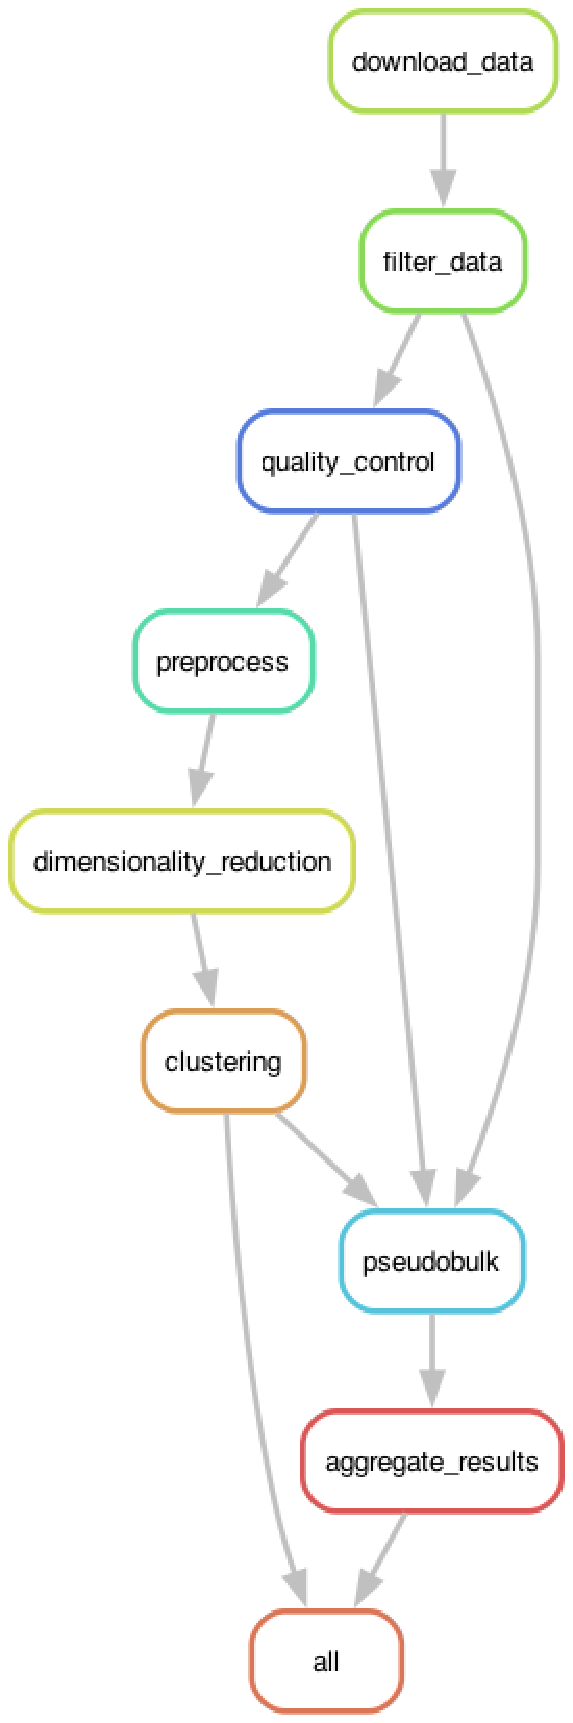
\includegraphics[width=0.375\linewidth]{figures/08/rnaseq-DAG.pdf}
\caption[Execution graph for RNA-seq example]{The execution graph for the RNA-seq analysis workflow visualized as a DAG.}
\label{rnaseq-DAG-fig}
\end{figure}

The \texttt{Snakemake} file is substantially larger for this complex workflow; to keep it from being even longer, we can also move some of the rules into separate rules files using the following syntax within the \texttt{Snakemake} file:

\begin{lstlisting}[style=Python]
# Include modular rule files
include: "rules/common.smk"
include: "rules/preprocessing.smk"
include: "rules/pseudobulk.smk"
include: "rules/per_cell_type.smk"
\end{lstlisting}

\subsection{Pipeline optimization}

The first time that I ran this workflow using Snakemake, I noticed that it was substantially slower than when I ran it using the custom workflow engine.  When I asked my chatbot about this, it gave me a reasonable answer:

\begin{quote}
The \textit{Snakemake} rules don't specify a threads directive. By default, \textit{Snakemake} runs each job with 1 thread, which limits parallelization of computationally intensive operations like neighbor computation and UMAP (which use numba internally).\index{parallelization}
\end{quote}

I asked the AI agent to fix this, and it returned the following change:

\begin{quote}
Fixes applied:

\begin{enumerate}
\item Added threads: 8 to dimensionality\_reduction rule
\item Added threads: 8 to quality\_control rule (Scrublet)
\item Added threads: 4 to preprocess rule
\item Set NUMBA\_NUM\_THREADS and OMP\_NUM\_THREADS environment variables in dimred.py
In contrast, tasks run in the main process have access to all CPUs by default, which is why it was faster.
\end{enumerate}
\end{quote}

This involved creating rules like this one:

\begin{lstlisting}[style=Pythonshort]
rule dimensionality_reduction:
...
    threads: 8
\end{lstlisting}

The \texttt{dimred.py} script then uses the \texttt{snakemake.threads} variable to set the relevant environment variables. This rule defines the ideal situation: that is, what is the maximum number of threads that our code can take advantage of?  In general a number from 4-8 is optimal here, given the overhead that comes with multithreading (as I will discuss further in the later chapter on Performance Optimization).  While this might seem problematic (e.g., what if there are only four cores available?), \textit{Snakemake} deals with it gracefully.  If there are more cores available than the limit, then \textit{Snakemake} will (if appropriate) spawn multiple processes in parallel. If there are fewer than the number requested, it will simply use what is available. There is a separate command line argument to \textit{Snakemake} (\texttt{--cores}) that specifies the maximum number of cores that can be utilized on the computer.\index{multithreading}

\subsection{Parametric sweeps}

A common pattern in some computational research domains is the \textit{parametric sweep}, where a workflow is run using a range of values for specific parameters in the workflow.  A key to successful execution of parametric sweeps is proper organization of the outputs so that they can be easily processed by downstream tools.  \textit{Snakemake} provides the ability to easily implement parametric sweeps simply by specifying a list of parameter values in the configuration file.  For example, let's say that we wanted to assess predictive accuracy using several values of the regularization parameter (known as \textit{alpha}) for a ridge regression model.  We could first specify a setting within our \texttt{config.yaml} file containing these values:\index{regularization}

\begin{lstlisting}[style=yaml, numbers=none, caption={}]
ridge_alpha:
  - 0.1
  - 1.0
  - 10.0
\end{lstlisting}

We would then add wildcards to the inputs and/or outputs for the relevant rules, expanding the parameters so that each unique value (e.g. each of our different models) becomes an expected input/output:

\begin{lstlisting}[style=Python]
rule all:
    input:
        expand("results/ridge/alpha_{param}/model.pkl",
               param=config["ridge_alpha"])

rule train:
    input:
        "data/train.csv"
    output:
        "results/ridge/param_{param}/model.pkl"
    shell:
        "python train.py --model ridge --param {wildcards.param} -o {output}"
\end{lstlisting}

It is also possible to generate parameters based on earlier steps in the workflow. In our RNA-seq workflow, we determine in an earlier step which specific cell types to include, based on their prevalence in the dataset.  These cell types are then used to run the per-cell-type analyses in a later step, executing the same enrichment and pathway analyses on each of the selected cell types.  This kind of data-dependent computational graph requires the use of the advanced checkpointing features in \textit{Snakemake}.

One could certainly perform the parametric sweep outside of the workflow engine (e.g. by running several \textit{Snakemake} jobs for each set of values or by looping over the values within the main job script rather than at the workflow layer). However, there are several advantages to doing it within a coherent workflow. First, it ensures that all of the runs are performed using exactly the same software environment and workflow.  If the different parameter settings were run in different workflows, then it is possible that the software environment could change between runs, so one would need to do additional validation to ensure that it was identical across runs.  Second, it maximizes the use of system resources, since the workflow manager can optimally split the work across the available number of cores/threads.  Running multiple snakemake jobs at once has the potential to request more threads than available, which can sometimes substantially reduce performance.  Manually managing system resources can require substantial effort.  Third, it enables the use of values from earlier workflow steps to determine the parameters for sweeping at later layers, as in the cell-type example above.  Finally, it makes incremental changes easy and economical; if one additional value of the parameter is added, \textit{Snakemake} will only run the computations for the new value.

\section{Workflow testing strategies}

Software testing is just as essential for workflow development as it is for any other kind of software, but there are a few particular issues that are uniquely relevant for testing workflows:

\begin{itemize}
\item It may not be possible to perform testing using realistic datasets, either due to data size or to restrictions on data access.
\item Smaller test datasets may not fully exercise the same behaviors as real datasets.
\item Results are often non-deterministic, such as those involving Monte Carlo simulations or search processes with random initialization, making it difficult to test for a specific outcome.\index{Monte Carlo simulation}
\item These tests often require comparison of equality between floating point numbers, but those require some degree of tolerance for floating point errors, which can be difficult to choose in order to simultaneously catch real errors and avoid false alarms.
\item Scientific workflows often take a very long time to run (hours or even days), making full integration tests infeasible.\index{testing!integration}
\item Finally, in scientific workflows we often don't know the right answer to expect from code, if we are performing operations that have never been done before.
\end{itemize}

I will leave the question of analytic accuracy to be addressed in the following chapter on validation. Here I will focus primarily on unit testing of workflow components and integration testing using a minimal test dataset.\index{testing!unit}

\subsection{Generating tests using AI agents}

Because I didn't use test-driven development to generate this workflow, I was faced with the task of having to generate a substantial amount of testing code for the completed workflow. To get a feel for the scale, the source code for our RNA-seq analysis contained 83 functions defined across 13 files.  In total these files included 3,239 lines, though there are actually many fewer lines of code, since many lines are blank or contain comments.  In addition many individual commands are split across lines to increase readability.  Using the \href{https://radon.readthedocs.io/en/latest/}{\textit{radon}} package for source code analysis, we can compute the \textit{logical lines of code}, which is the number of executable statements:\index{test-driven development}

\begin{lstlisting}[style=shellshort]
$  uv run radon raw *.py | awk '/LLOC:/ {sum += $2} END {print sum}'
1038
\end{lstlisting}

Thus, we need to generate tests for 83 functions comprising more than 1000 statements!  As I discussed in Chapter 4, we can use AI tools to help generate test code, though this code \textit{must} be examined in detail by a knowledgeable human in order to ensure that the tests adequately exercise the relevant functions.

I started by generating a Markdown file specifying the test framework:

\begin{lstlisting}[style=transcript]
This is a set of implementations of an analysis workflow for single-cell RNA-seq data analysis. These are meant to exemplify different ways of building a workflow.  The main goal of this development project is to develop a testing framework for this workflow.  This will involve two main steps:

- develop unit tests for the functions defined within src/example_rnaseq
- develop integration tests for the snakemake workflow defined in snakemake_workflow

Some of these tests can be performed using automatically generated data. However, the integration tests will require a test dataset. this should be based on the actual data that can be found at $DATADIR/dataset-OneK1K_subset-immune_raw.h5ad.  To minimize the size of this dataset, we should first select a subset of 30 donors from the dataset.  we should look for donors that vary in the number of cells, with some having high numbers and some having low numbers. The donors should also vary in age so that the subset covers the entire distribution of ages in the dataset. then we should select a subset of about 500 genes.  these should include:

- a set of genes from a pathway (TNF-alpha Signaling via NF-KB) known to be associated with aging, found in tests/data/HALLMARK_TNFA_SIGNALING_VIA_NFKB.v2025.1.Hs.json
- a set of about 200 other highly variable genes
- a set of about 100 weakly variable genes

This dataset should be saved to tests/data/testdata.h5ad.

## Coding guidelines

- Think about the problem before generating code.
- Write code that is clean and modular. Prefer shorter functions/methods over longer ones.
- Prefer reliance on widely used packages (such as numpy, pandas, and scikit-learn); avoid unknown packages from Github.
- Do not include *any* code in `__init__.py` files.
- Use pytest for testing.
- Use functions rather than classes for tests. Use pytest fixtures to share resources between tests.
\end{lstlisting}

My agent took about 20 minutes to generate an entire test framework for the code, comprising 215 test functions and 19 test fixtures.  Interestingly, the agent disregarded my instructions to use functions rather than classes for tests, generating 78 test classes.  While I usually prefer tests to be in pure functions rather than classes so that novices can more easily understand them, I decided in this case to stay with the class-based implementation since I don't mind it and it does make the organization of the tests a bit cleaner.

The initial test set for this project had no tests for one of the modules, and other modules with significant portions untested.  I was able to improve this by having the agent analyze the code coverage report and identify important parts of the code that were not currently covered, which moved the test coverage from 69\% to 88\% of the 870 statements in the code that were identified by the \texttt{coverage} tool.\index{code coverage}

\subsection{Avoiding the happy path}

Because it is essential for AI-generated tests to be assessed by a knowledgeable human, I proceeded to read all of the tests that had been generated by the agent.  Fortunately they were all easily readable and clearly named, which made it relatively easy to see some potential problems right away. Several kinds of issues arose.

Because AI agents have a strong tendency to generate tests that pass, they will sometimes miss potential problems - this is commonly referred to as following the ``happy path''. Several of the tests performed very minimal checking of outputs that would miss potential problems.  For example, it generated the following test which, according to its name, should test whether a PCA embedding is generated using the \textit{harmonypy} package:

\begin{lstlisting}[style=Python]
def test_creates_harmony_embedding(self, adata_with_pca):
        """Test that Harmony creates a new embedding."""
        adata, use_rep = run_harmony_integration(adata_with_pca.copy())

        if use_rep == "X_pca_harmony":
            assert "X_pca_harmony" in adata.obsm
            assert adata.obsm["X_pca_harmony"].shape[0] == adata.n_obs
\end{lstlisting}

The \texttt{use\_rep} variable contains ``X\_pca\_harmony'' if the \textit{harmonypy} package is installed and successfully applied to the data, otherwise it falls back on standard PCA and sets \texttt{use\_rep} to ``X\_pca''.  But it's clear here that this package only checks for the harmony embedding in the case that it was successfully created (`if use\_rep == ``X\_pca\_harmony'''), in which case it makes sure that it is present in the dataset and has the right shape. Thus, the test could pass even if the harmony embedding was not successfully created.  Here is the improved version to address this issue:

\begin{lstlisting}[style=Python]
def test_creates_harmony_embedding(self, adata_with_pca):
        """Test that Harmony creates a new embedding with correct shape."""
        pytest.importorskip("harmonypy")

        adata, use_rep = run_harmony_integration(adata_with_pca.copy())

        assert use_rep == "X_pca_harmony"
        assert "X_pca_harmony" in adata.obsm
        assert adata.obsm["X_pca_harmony"].shape[0] == adata.n_obs
        assert adata.obsm["X_pca_harmony"].shape == adata.obsm["X_pca"].shape
\end{lstlisting}

In other cases, the tests that were generated were too minimal, allowing obvious failure cases to pass. For example, the integration test named ``test\_pseudobulk\_pipeline\_runs'' included the following code:

\begin{lstlisting}[style=Python]
result = run_pseudobulk_pipeline(
            adata,
            group_col="cell_type",
            donor_col="donor_id",
            metadata_cols=["development_stage", "sex"],
            min_cells=1,  # Low threshold for test data
            figure_dir=temp_output_dir,
        )

        # Check outputs
        assert result is not None
        assert result.n_obs > 0
        assert "n_cells" in result.obs.columns
        assert "cell_type" in result.obs.columns
        assert "donor_id" in result.obs.columns
\end{lstlisting}

Pseudobulking is an operation that should summarize all cells of a given type for each donor, but none of the test conditions actually check that it has been properly applied.  In fact, these tests could pass if \texttt{run\_pseudobulk\_pipeline()} simply passed the original data back without doing anything to it!  This is a case where domain knowledge is essential to get the tests right and avoid the happy path.  In several other cases the tests called \texttt{pytest.skip()} (which causes the test to be skipped) for outcomes that really should have triggered a test failure.  For example, it skipped the integration tests for the full dataset if the dataset hadn't already been created, and it also skipped the \textit{Snakemake} integration functions if the \textit{Snakemake} call failed (which it initially did because of a missing argument).\index{pytest}

These examples highlight the need to closely examine the test code that is generated by AI agents.  However it's worth noting that although it took a significant amount of human time to read over the AI-generated tests, the time spent was still far less than if I had undertaken writing the test code without AI assistance, and the coding agent was also able to fix all of the issues to my satisfaction after I raised them. 

\begin{framed}
\textbf{Tip}\\
Break the code on purpose and see if the tests catch it.  That's a powerful way to see whether AI-generated tests are actually valid.
\end{framed}

\subsection{Property-based testing for workflows}\index{testing!property-based}

The tests initially developed for this workflow were built around the known characteristics of the expected data. However, there are many ``unknown unknowns'' when it comes to input data, and it's important to make sure that the code deals gracefully with problematic inputs. We can test this using a \textit{property-based testing} approach; as I discussed in Chapter 4, this involves the generation of many different datasets that follow a particular specification, and checking whether the code deals with them appropriately.  When I asked the coding agent to identify plausible candidates for property-based testing using the Hypothesis package, it generated \href{https://github.com/BetterCodeBetterScience/example-rnaseq/blob/main/tests/test\_hypothesis.py}{tests} centered on several different properties:

\begin{itemize}
\item Proper parsing of a range of filenames for the BIDS format parser used in caching\index{BIDS (Brain Imaging Data Structure)}
\item Consistency of hashing operations
\item Proper JSON serialization of a range of values
\item Proper processing of input lists with a range of inputs
\end{itemize}

These are all good applications of property-based testing because they focus on invariant features that should be true regardless of the inputs (i.e. the same input should always generate the same hash, or loading a serialized dataset should return the same values as the original). I further pushed it to identify plausible candidates for testing of the effects of numerical edge cases, such as division by zero, which is another valuable use case for property-based testing. This paid off when the property-based tests generated by the agent identified a bug that had not been caught by the previous tests:

\begin{lstlisting}[style=transcript]
The property-based test found a real bug! The prepare\_enrichr\_plot\_data function produces infinity when computing -log10(0) for zero p-values. The GSEA version handles this with + 1e-10, but the Enrichr version doesn't.
\end{lstlisting}

This highlights the utility of property-based testing alongside standard unit tests.

% \chapter{Validating scientific software}

So far I have focused very heavily on \textit{reproducibility}, that is, the ability to generate the same answer when code is run repeatedly.  However, it's easy to reliably generate the wrong answer!  In measurement theory there is a fundamental distinction between \textit{reliability} and \textit{validity}: Reliability means performing the same method repeatedly results in highly similar results, whereas validity refers to whether the estimated result is close to the true result.  In this chapter we turn to the \textit{validation} of scientific software, by which I mean the degree to which it performs the intended task as expected and gets the answers right.\index{reproducibility}

\section{Creating simulations}

Creating simulations is perhaps the most important tool that computers offer the scientist, as captured in a well-worn quote by \citep{Press:1992}:

\begin{quote}
offered the choice between mastery of a five-foot shelf of analytical statistics books
and middling ability at performing statistical Monte Carlo simulations, we would surely\index{Monte Carlo simulation}
choose to have the latter skill. (p.691)
\end{quote}

Simulations are indeed a powerful way to understand a system even when it's not analytically tractable.  More importantly, they are generally the only way that we can establish \textit{ground truth} against which we can compare our models.  We can generate data where we know the answer, run our analysis on those simulate data, and make sure that the analysis provides us with the correct answer.  As scientists we never know the true process that generates our data, but with simulations we can have complete control over the data generation process.

My previous book, \textit{Statistical Thinking} \citep{Poldrack:2023stats}, gives an \href{https://statsthinking21.github.io/statsthinking21-core-site/resampling-and-simulation.html}{overview} of how to use simulations in the context of statistics; here I will focus primarily on the use of simulation in the context of software validation, but I recommend that book for background reading if you aren't already familiar with the concept of a statistical distribution.

\subsection{Generating random numbers}

The most fundamental requirement in nearly any simulation is the ability to generate random numbers.\footnote{For the sake of convenience I will use the term \textit{random numbers} for series of numbers generated by a computational algorithm, but it is more precise to call them \textit{pseudorandom numbers}, because the series will ultimately repeat after a very long time.  See Chapter 3 of \cite{Knuth:1981aa} for a detailed discussion.} What makes a series of numbers \textit{random} is that it is impossible (or at least nearly impossible) to predict the next value in the series.  Random numbers are defined by the \textit{distribution} that characterizes them, which is a mathematical function that describes the ``shape'' of the data when they are summarized according to the relative frequency of different values or ranges of values.  Picking the correct distribution is essential to ensure that any simulation performs as advertised.  Fortunately, there are lots of existing packages that provide tools to generate random numbers for nearly any distribution; I will focus on the \textit{NumPy} package here since it is the most commonly used.\index{NumPy}

The simplest distribution is the \textit{uniform} distribution, in which any possible value (within a particular range for continuous values) has the same probability of occurring.  We can generate uniform random variates by first creating a random number generator object using \texttt{np.random.default\_rng()}, and then calling \texttt{rng.uniform()} which returns random samples from the distribution:\index{generator}

\begin{lstlisting}[style=replshort]
>>> rng = np.random.default_rng()
>>> rng.uniform(size=10)
array([0.2540087 , 0.5284475 , 0.32548277, 0.74116308, 0.82750185,
       0.11758439, 0.06351991, 0.24068558, 0.87900871, 0.36374554])
\end{lstlisting}

In this case, \texttt{rng.uniform()} by default generates floating point values that fall within [0, 1]; this can be changed using the location and scale parameters to the function.  If we generate a large number of these then we can create a distribution plot (often called a \textit{histogram}) showing how the numbers are distributed, as shown in Figure~\ref{DistPlots-fig}.

\begin{figure}[!htbp]
\centering
\includegraphics[width=0.75\linewidth]{files/multiple_distributio-e69093f01223e1ab5a2da8234372dfed.png}
\caption[Distribution plots from six different distributions]{Distribution plots for 1,000,000 random samples from each of six different distributions.}
\label{DistPlots-fig}
\end{figure}

For purposes of reproducibility it's often useful to be able to regenerate exactly the same series of random samples. We can do this by specifying a \textit{random seed}, which gives the random number generating a starting point. If you are going to do simulations then it is important to understand the specific random number generator that your code will use.  Previously it was common to use the global \textit{NumPy} random seed function (\texttt{np.random.seed()}) to set the seed, and this is still necessary when using packages that access the global random number generator. However, the best practice is to generate a random number generator object (using \texttt{np.random.default\_rng()}), and then call the methods of that object to obtain random numbers, as I did above.  This prevents surprises in case other functions modify the global seed, helps isolate your specific generator, and enables multiple parallel generators.  Here is an example:

\begin{lstlisting}[style=replshort]
>>> rng = np.random.default_rng(seed=42)
>>> rng.uniform(size=4)
array([0.77395605, 0.43887844, 0.85859792, 0.69736803])
\end{lstlisting}

If we run this again, we see that a different series of numbers is generated:

\begin{lstlisting}[style=replshort]
>>> rng.uniform(size=4)
array([0.09417735, 0.97562235, 0.7611397 , 0.78606431])
\end{lstlisting}

However, if we generate another object with the same seed, we will see that it gives us the same values as above:

\begin{lstlisting}[style=repl]
>>> rng2 = np.random.default_rng(seed=42)
>>> rng2.uniform(size=4)
array([0.77395605, 0.43887844, 0.85859792, 0.69736803])

>>> rng2.uniform(size=4)
array([0.09417735, 0.97562235, 0.7611397 , 0.78606431])
\end{lstlisting}

Setting random seeds is important to enable exact reproducibility of results generated using random numbers. However, it's also important to ensure that one's results are robust to the choice of random seed, as I will discuss later in the context of machine learning analyses.\index{machine learning}

\subsection{Choosing a distribution}

Choosing the right distribution for a simulation often comes down to understanding the data-generating process and kind of data that are being modeled.  Here are a few examples of distributions and their common use cases:

\textit{Discrete outcomes}

\begin{itemize}
\item \textit{Bernoulli}:  A distribution of binary outcomes (often interpreted as success vs failure) given a probability of a positive outcome.

\begin{itemize}
\item Examples: Whether a patient responds to a given treatment, whether a hard drive fails within a particular period of time.
\end{itemize}


\item \textit{Binomial}: A distribution of the number of successes across a specific number of Bernoulli trials, given a probability of a positive outcome.

\begin{itemize}
\item Examples: The number of patients who respond to treatment in a clinical trial treatment group, the number of hard drives that fail within a particular period of time at a particular data center
\end{itemize}


\item \textit{Categorical}: A distribution with several distinct possible outcomes, each of which has a particular probability:

\begin{itemize}
\item Examples: Eye color across a population, programming languages used by programmers in a company
\end{itemize}


\item \textit{Uniform}: A specific form of a discrete categorical variable with equal probability

\begin{itemize}
\item Examples: equiprobable physical outcomes such as a dice roll.
\end{itemize}


\item \textit{Multinomial}: A multivariate generalization of the binomial, representing the counts of multiple possible outcomes across a set of independent trials with fixed probabilities of each outcome.

\begin{itemize}
\item Examples: Frequencies of types of stars in a galaxy, frequencies of cell types in a tissue sample
\end{itemize}
\end{itemize}

\textit{Continuous outcomes}:

\begin{itemize}
\item \textit{Uniform}: A distribution with equal probability density for all values within the range.

\begin{itemize}
\item Examples: probabilities of events when there is no prior knowledge, equiprobable continuous physical outcomes
\end{itemize}


\item \textit{Beta}: A generalization of the uniform distribution that models the probability of values within a range but has two parameters that allow different values across the range to have different probabilities.

\begin{itemize}
\item Examples: Prior probabilities in a Bayesian model, proportions of time spent in a particular state.\index{Bayesian inference}
\end{itemize}


\item \textit{Normal} (or \textit{Gaussian}): A symmetric distribution centered around a mean, which commonly arises when an outcome is generated based on many small additive contributions. The Central Limit Theorem explains why this occurs so frequently, as it should arise for sums of independent random variables sampled from \textit{any} distribution, as long as the sample size is large enough and the distribution has finite variance.

\begin{itemize}
\item Examples: Height of individuals in a population, measurement errors for continuous variables
\end{itemize}


\item \textit{Log-normal}:  Distribution of positive continuous values whose logarithm is normally distributed.  It reflects the expected values of a product of independent random variables.

\begin{itemize}
\item Examples: Wealth and income distributions in a population, biological growth processes
\end{itemize}
\end{itemize}

\textit{Count data}:

\begin{itemize}
\item \textit{Poisson}: This is a distribution of counts of events within a fixed interval assuming that the events are independent and occur at a constant rate. Unlike the binomial there is no limit on the number of events that can occur, and it is the limiting case of the Binomial when the sample size $n$ approaches infinity and the probability $p$ approaches zero (and $n * p$ remains constant).

\begin{itemize}
\item Examples: The number of atoms decaying within a particular period, the number of emails that a person receives within a day
\end{itemize}


\item \textit{Negative binomial}: A distribution that models count data that are \textit{overdispersed}, meaning that their variance is greater than their mean.  It can also be interpreted as representing the number of failures that occur before a given number of successes.

\begin{itemize}
\item Example: Commonly used in genomics to model read counts in genomic sequencing.
\end{itemize}
\end{itemize}

\textit{Waiting time data}:

\begin{itemize}
\item \textit{Exponential}: A distribution of waiting times in a process governed by a Poisson distribution, with a constant \textit{hazard rate} (i.e. the probability of happening in the next period is independent of whether the event has happened yet).

\begin{itemize}
\item Examples: Time between atomic decays, time between hard drive failures
\end{itemize}


\item \textit{Weibull}: A generalization of the exponential distribution that allows modeling of waiting times with increasing, constant, or decreasing hazard rates.

\begin{itemize}
\item Examples: Response times in human behavior, time to failure for some electronic devices
\end{itemize}
\end{itemize}

It is essential to choose the right distributions for a simulation; otherwise the results may be misleading at best or meaningless at worst.  

\subsection{Simulating data from a model}

In some cases, we want to simulate data that have particular structure in order to test whether our code can properly identify the structure in the data. Depending on the kind of structure one needs to create, there are often existing tools that can help generate the data.  For example, the \textit{scikit-learn} package has a large number of data generators that are often useful, either on their own or as a starting point to develop a custom generator.  Similarly, the \textit{NetworkX} graph analysis package has a large number of graph generators available.\index{scikit-learn}

Let's say that we have developed a function that estimates an undirected graph from network data.  We would like to generate data from a known graph and then examine our ability to identify the true edges in the graph from the data. For this, we can use an existing graph; I chose one based on a dataset of gene expression in E. coli bacteria that was used by \cite{Schafer:2005aa} and is shared via the \textit{pgmpy} package:

\lstinputlisting[style=Python, firstline=103, lastline=118]{../src/bettercode/network_recovery.py}

Figure~\ref{ecoli-fig} shows the resulting rendering of that network, which has 46 nodes (representing individual genes) and 70 directed edges (representing causal relationships on gene expression between nodes).  This is a \textit{directed acyclic graph} (or DAG), in which the edges have arrows that reflect causal influences from one node to another. However, our analysis method will focus only on the presence/absence of edges and not their direction, hence the term \textit{undirected graph}.  \index{DAG (directed acyclic graph)}

\begin{figure}[!htbp]
\centering
\includegraphics[width=0.75\linewidth]{files/ecoli-6b54c902b92b42e2bae553ac97df4d9d.png}
\caption[Plot of graphical model for E. Coli gene expression]{A plot of the graphical model for the E. Coli gene expression data generated by \cite{Schafer:2005aa}.}
\label{ecoli-fig}
\end{figure}

Given this graph, we then need to generate data for expression of each gene that reflect the causal relationships between the genes.  To do this, we use \textit{Numpy} to generate multivariate normal data with a given covariance structure that is based on the known graph.  First we need to generate the covariance matrix; to do this, we leverage the fact that the inverse of the covariance (known as the \textit{precision}) is a representation of direct influences. Since we know these direct influences (based on the graph), we can generate the precision matrix using those known edges and then invert it to obtain the covariance matrix:

\lstinputlisting[style=Python, firstline=24, lastline=41]{../src/bettercode/network_recovery.py}

We can then create a function that uses this covariance matrix to generate random samples from a multivariate normal distribution:

\lstinputlisting[style=Python, firstline=44, lastline=48]{../src/bettercode/network_recovery.py}

Now that we have the dataset we can test out our estimation method. We will use a very simple method that involves computing the \textit{partial correlation} between each pair of edges. This is the correlation after having removed the influence of all other edges, and thus reflects the unique direct relationship between edges, as opposed to the standard correlation which reflects both direct and indirect relationships.  The partial correlation is simply a scaled version of the inverse covariance (precision), which we can compute directly from the data.  Note that this is a suboptimal method for computing the partial correlation, which will fail when there are more nodes than data points; I use it here as a simple example.  Our function computes the partial correlation and then returns the edges whose partial correlation exceeds a specified threshold:

\lstinputlisting[style=Python, firstline=51, lastline=68]{../src/bettercode/network_recovery.py}

The results from this analysis include a list of all of the edges that were identified from the data using causal discovery, which we can summarize to determine how well the model performed:

\lstinputlisting[style=Python, firstline=71, lastline=96]{../src/bettercode/network_recovery.py}

\begin{lstlisting}[style=shell]
single run @ signal=0.4, threshold=0.15:
  70 true edges, discovered 64 edges
  63 true positives, 1 false positives
  recall=90.00%  precision=98.44%  fdr=1.56%  f1=94.03%
\end{lstlisting}

The results showed that the model performed fairly well, detecting 90\% of the true edges but also detecting one false edge.  In general we would want to do additional validation to make sure that the results behave in the way that we expect. For example, we would expect better model performance with stronger signal, and we would expect fewer nodes identified when the p-value threshold is more stringent.  We can use the functions generated above to run a simulation of this:

\lstinputlisting[style=Python, firstline=114, lastline=135]{../src/bettercode/network_recovery.py}

We can then plot these results, as shown in Figure~\ref{simresults-fig}.  The results confirm that the model is performing as expected, with increasing recall as a function of increasing true signal and decreasing FDR threshold.

\begin{figure}[!htbp]
\centering
\includegraphics[width=0.75\linewidth]{files/network_recovery_performance.png}
\caption[Plot of true/false discovery rate as threshold increases]{A plot of observed true positive rate (TPR) and false discovery rate (FDR) at increasing signal levels for varying correlation thresholds.}
\label{simresults-fig}
\end{figure}

\subsection{Simulating data based on existing data}

It's very common for researchers to collect a dataset of interest and then develop code that implements their analysis on that dataset to ask their questions of interest. However, this approach raises a concern that the choices made in the course of analysis might be biased by the specific features of the dataset \citep{Gelman:2014aa}.  In particular, decisions might be made that reflect the noise in the dataset, rather than the true signal, which is often referred to as \textit{overfitting} (discussed further below). In some fields (particularly in physics) it is common to perform \textit{blind analysis} \citep{MacCoun:2015aa}, in which analysts are given data that are either modified or relabeled, in order to prevent them from being biased by their hypotheses.  One way to achieve this in the context of data analysis is to develop the code using a simulated dataset that has some of the same features as the real dataset, such that one can implement the code, validate it, and then immediately apply it to the real data once they are made available.  To achieve this, one needs to be able to generate simulated data based on an existing dataset; for blind analysis, the generation of the simulated data should be performed by a different member of the research team. For example, in some cases I have generated the simulated data for a study based on the real data and provided those to my students, only providing them with the real data once the code was implemented and validated.\index{overfitting}

The important question in generating simulated data from real data is what specific features one intends to capture from the real data. This generally will require some degree of domain expertise in order to understand the features of the data.  Some common features that one might wish to replicate are:

\begin{itemize}
\item Data types (e.g. categorical, integer, floating point)
\item Marginal distributions of the values (minimally the summary statistics, preferably the shape)
\item Joint distributions of the variables (e.g. capturing correlations between variables)
\end{itemize}

It's generally important to avoid including features in the model that are directly relevant to the hypothesis.  For example, if the hypothesis relates to correlations between specific variables in the dataset, then the correlation in the simulated data should \textit{not} be based on the correlation in the real data, lest the analysis be biased.

Here I will focus primarily on tabular data; while there are simulators to generate more complex types of data, such as genome wide association data \citep{Purcell:2007aa} and functional magnetic resonance imaging data \citep{Ellis:2020aa}, these require substantial domain expertise to use properly, whereas tabular data are widely applicable.  For simple datasets it may be most appropriate to generate simulated data by hand; here I will use the \textit{Synthetic Data Vault} (SDV) Python package (sdv.dev), which has powerful tools for generating many kinds of synthetic data.\index{Python}

As an example, I will use the Eisenberg data that you have already seen on a couple of occasions. I'll start by picking out a few variables and then using \textit{SDV} to create a synthetic dataset whose distributions for each variable match those in the original, but the columns are generated independently, which removes any correlations between columns. After loading and combining the demographic and behavioral data frames, selecting a few important variables, and joining them into a single frame (\texttt{df\_orig}), I then use \textit{SDV} to generate simulated data for each variable, shuffling each column after generation to destroy any correlations:

\begin{lstlisting}[style=Python]
from sdv.single_table import GaussianCopulaSynthesizer
from sdv.metadata import Metadata

def generate_independent_synthetic_data(df: pd.DataFrame, random_seed: int = 42) -> pd.DataFrame:
    """
    Generate synthetic data where all variables are independent.
    
    Uses SDV to model the full dataset, then shuffles each column 
    independently to break all correlations while preserving marginal distributions.
    
    Args:
        df: Original dataframe to generate synthetic version of.
        random_seed: Random seed for reproducibility (default: 42).
        
    Returns:
        Synthetic dataframe with same shape and column names as input,
        but with independent variables.
    """
    # Suppress the metadata saving warning
    warnings.filterwarnings('ignore', message='We strongly recommend saving the metadata')
    
    # Set random seed
    if random_seed is not None:
        np.random.seed(random_seed)
    
    # Create metadata for the full dataset
    metadata = Metadata.detect_from_dataframe(
        data=df,
        table_name='full_data'
    )
    
    # Create synthesizer for the full dataset
    synthesizer = GaussianCopulaSynthesizer(
        metadata,
        enforce_rounding=False,
        enforce_min_max_values=True,
        default_distribution='norm'
    )
    
    # Fit synthesizer to the full dataset
    synthesizer.fit(df)
    
    # Generate synthetic data
    df_synthetic = synthesizer.sample(num_rows=len(df))
    
    # CRITICAL: Shuffle each column independently to break all correlations
    # This preserves the marginal distribution of each variable but eliminates dependencies
    for col in df_synthetic.columns:
        shuffled_values = df_synthetic[col].values.copy()
        np.random.shuffle(shuffled_values)
        df_synthetic[col] = shuffled_values
    
    return df_synthetic
\end{lstlisting}

We can then visualize the correlations and distributions for the original data and the synthetic data; in Figure~\ref{sdvdist-fig} we see that the distributions in the synthetic data are very similar to those in the original data, while in Figure~\ref{sdvcorrs-fig} we see that the synthetic data do not include the original correlations.

\begin{figure}[!htbp]
\centering
\includegraphics[width=0.8\linewidth]{files/sdv_distributions-497ca4c3be03a7f8ae7272ccc1ea7da5.png}
\caption[Comparison of distributions for original and synthetic data]{A comparison of the distributions of the original and synthetic data for several of the variables in the example dataset.}
\label{sdvdist-fig}
\end{figure}

\begin{figure}[!htbp]
\centering
\includegraphics[width=0.8\linewidth]{files/sdv_correlations-acd7b2adfdd59eba7551a96f501a039d.png}
\caption[Comparison of correlation matrices for original and synthetic data]{A comparison of the correlations matrices for the numeric variables in the original and synthetic data.}
\label{sdvcorrs-fig}
\end{figure}

The \textit{SDV} package also offers many additional tools for more sophisticated generation of synthetic data.  We will see below additional ways to use synthetic data for validation of scientific data analysis code.

\section{Estimating model parameters}

It is very common in science to collect data and then use those data to estimate the parameters for a given model, and it's important to ensure that the estimates are valid.  Given the central role of parameter estimation in code testing and validation, I now dive into the various methods that one can use to estimate model parameters, and show examples of how we might validate them. In addition to estimating model parameters, we generally also want some kind of way to quantify the uncertainty in our estimates. That is, rather than thinking of the parameter estimate as a single point value, we can ask: What range of values for the parameter are consistent with the data?  This is often expressed using \textit{confidence intervals}, though I will discuss below the ways that these are often misunderstood.

A central idea in this section will be the notion of \textit{parameter recovery}: that is, how well can our estimation procedure recover the true parameter values using simulated data? This is particularly important in cases where we don't have statistical guarantees on the unbiasedness of our estimates. As we will see, simulation provides a powerful tool to assess parameter recovery performance for any model.  We will look at three different ways that one can estimate model parameters from data, whose applicability depends on the nature of the model being used.

\subsection{Closed-form estimates}

In some cases parameter estimates can be obtained using a closed form analytic solution.  We will use the normal distribution as an example.  This distribution has two parameters: a \textit{mean} (which is a \textit{location} parameter) that specifies where the center of the distribution falls, and a \textit{standard deviation} (which is a \textit{scale} parameter) that specifies the width of the distribution.  The probability function for the normal distribution is:

\begin{equation}
p(x \mid \mu, \sigma) = \frac{1}{\sigma \sqrt{2\pi}} \exp\left(-\frac{(x - \mu)^2}{2\sigma^2} \right)
\end{equation}

where $\mu$ is the mean and $\sigma$ is the standard deviation.

Our goal in estimating model parameters is to find estimates (in this case for the mean and standard deviation) that maximize some measure of \textit{goodness of fit} with respect to the data, or equivalently, minimize some measure of \textit{error}.  Since we don't want positive and negative errors to cancel each other out, we need a measure of error that is uniquely positive regardless of the direction of the error.  The most common measure in statistics is the \textit{mean squared error}:

\begin{equation}
\text{MSE} = \frac{1}{n} \sum_{i=1}^{n} (y_i - \hat{y}_i)^2
\end{equation}

where $y_i$ is the value for the i-th observation, $\hat{y}_i$ is the estimated value for that observation from the model, and $n$ is the sample size.  In the case of the normal distribution, $\hat{y}_i$ is the same for each observation: the mean.  We can
estimate the mean for the sample using the closed form solution:

\begin{equation}
\bar{y} = \frac{1}{n} \sum_{i=1}^{n} y_i
\end{equation}

where $\bar{y}$ is the mean.  We can then compute the standard deviation using this estimated mean:

\begin{equation}
s_y = \sqrt{\frac{1}{n-1} \sum_{i=1}^{n} (y_i - \bar{y})^2}
\end{equation}

Note that this is very similar to the mean squared error, differing in the presence of a square root as well as the use of $n - 1$ rather than $n$ in the demominator. The latter is meant to adjust for the fact that we lost one \textit{degree of freedom} when we estimated the mean from the same data and then used it to compute the standard deviation.  When the variance (the square of the standard deviation) is computed using this correction it will be \textit{unbiased}, meaning that its expected value will match the true variance of the population.  The standard deviation is still slightly biased, but less so than the one computed without the correction.

Figure~\ref{NormalDist-fig} shows an example of a histogram based on samples from a normal distribution, with the theoretical normal distribution based on the estimated sample mean and standard deviation overlaid.  Visually it's clear that the fitted distribution characterizes the overall shape well, even if it mismatches the shape at finer grain, due to sampling variability.

\begin{figure}[!htbp]
\centering
\includegraphics[width=0.5\linewidth]{files/normal_distribution-acc79d4904ef049b883835ad3db91243.png}
\caption[Histogram of normal samples with fitted distribution]{A histogram of 1000 samples from a standard normal distribution (with mean of zero and standard deviation of one), with the fitted normal distribution overlaid in red.}
\label{NormalDist-fig}
\end{figure}

\subsubsection{Quantifying uncertainty in closed-form estimation}

In general we want not just a point estimate for our parameter but also an estimate of our uncertainty in that estimate.  The \textit{confidence interval} is the most commonly used method for expressing uncertainty around an estimate, and with closed form expressions it's often possible to compute the confidence interval directly. A confidence interval is expressed in terms of a percentage, but the meaning of this percentage is often misinterpreted (see the discussion in my \textit{Statistical Thinking} for more on this).  The term ``95\% confidence interval'' seems to imply that it is an interval in which we have 95\% confidence that the true value of the parameter falls.  However, that violates the frequentist statistical logic that underlies the computation of the confidence interval, which treats the true value as fixed, and thus it either falls in the interval or it doesn't.  Instead, the more appropriate interpretation of a frequentist confidence interval is that it is the interval that would capture the true population mean 95\% of the time for samples from the same population.  I prefer to frame it in a slightly different, if somewhat less precise way: The confidence interval expresses the range of plausible values for the parameter given our data, and thus tells us something about the precision of our estimate:  All else being equal, a sample estimate with a narrower confidence interval is more precise than an estimate with a wider confidence interval.

Using our example from above, we can compute a confidence interval for our estimate of the sample mean.  This requires that we have a probability distribution that is associated with our statistic; in this case, the \textit{Student's t} distribution is appropriate since we have estimated the standard deviation as well as the mean.  The \textit{t} distribution has slightly wider tails than the normal distribution, which helps account for the added uncertainty in our estimate of the standard deviation.  The equation for the confidence interval around the mean using the \textit{t} distribution is:

\begin{equation}
\bar{y} \pm t_{\alpha/2, \, n-1} \cdot \frac{s_y}{\sqrt{n}}
\end{equation}

where $s_y$ is the sample standard deviation, $n$ is the sample size, and $t_{\alpha/2, \, n-1}$ is the \textit{critical value} of the \textit{t} distribution with $n - 1$ degrees of freedom at the $\alpha/2$ percentile. $\alpha$ defines our confidence level, and it is divided by two since we are interested in both the positive and negative directions.  In our case, this results in a confidence interval of [-0.09028, 0.03249].  We can use a simulation to confirm that this interval indeed captures the sample mean 95\% of the time for new samples from the same distribution:

\begin{lstlisting}[style=Python]
n_simulations = 100000
confidence_level = 0.95
alpha = 1 - confidence_level
random_state = 42
true_mean, true_sd = 0, 1
sample_size = 1000

# Track how many times the CI captures the true mean
captures = 0

# Run simulations
for i in range(n_simulations):
    # Draw a new sample from the population
    sample = norm.rvs(loc=true_mean, scale=true_sd, 
        size=sample_size, random_state=random_state)
    
    # Calculate sample statistics
    sample_mean_sim = np.mean(sample)
    sample_sd_sim = np.std(sample, ddof=1)
    
    # Calculate confidence interval
    df = sample_size - 1
    t_crit = t.ppf(1 - alpha/2, df)
    se = sample_sd_sim / np.sqrt(sample_size)
    margin = t_crit * se
    
    ci_low = sample_mean_sim - margin
    ci_high = sample_mean_sim + margin
    
    # Check if CI captures the true mean
    if ci_low <= true_mean <= ci_high:
        captures += 1

# Calculate coverage rate
coverage_rate = captures / n_simulations

print(f"Simulation results:")
print(f"Number of simulations: {n_simulations}")
print(f"Sample size per simulation: {sample_size}")
print(f"True population mean: {true_mean}")
print(f"Confidence level: {confidence_level * 100}%")
print(f"\nCoverage rate: {coverage_rate:.4f} ({coverage_rate * 100:.2f}%)")
\end{lstlisting}

\begin{lstlisting}[style=shell]
Simulation results:
Number of simulations: 100000
Sample size per simulation: 1000
True population mean: 0
Confidence level: 95.0%

Coverage rate: 0.9503 (95.03%)
\end{lstlisting}

Here we see that the observed proportion of samples where the sample mean falls within the confidence interval is very close to the 95\% that we expect based on statistical theory.

\subsubsection{The bootstrap as a general method for quantifying uncertainty}\index{bootstrap}

There are often cases where we don't have a sampling distribution that we can use to form a confidence interval.  In these cases,  we can use a technique known as the \textit{bootstrap}.  This method takes advantage of \textit{resampling}, meaning that we repeatedly draw samples with replacement from our full sample.  We can do this using the \texttt{scipy.stats.bootstrap()} function, which performs the bootstrap on a sample given any statistical function:\index{SciPy}

\begin{lstlisting}[style=Python]
from scipy.stats import bootstrap

# use the bias-corrected/accelerated method ('BCa')
res = bootstrap((normal_samples,), np.mean, confidence_level=0.95,      
    n_resamples=10000, method='BCa', random_state=random_state)

print(f'Bootstrap 95% CI for mean: '
    f'[{res.confidence_interval.low:.5f}, '
    f'{res.confidence_interval.high:.5f}]')
print(f'CI based on t-distribution: [{ci_lower:.5f}, {ci_upper:.5f}]')
\end{lstlisting}

\begin{lstlisting}[style=shell]
Bootstrap 95% CI for mean:  [-0.09104, 0.03078]
CI based on t-distribution: [-0.09028, 0.03249]
\end{lstlisting}

Here we see that the bootstrap procedure gives results that are very close to those obtained using the closed form solution, but has the advantage of being usable with nearly any statistic (except for those based on extreme values) regardless of whether or not there is a closed form estimator and/or the sampling distribution is analytically tractable.

Despite the challenges in interpreting frequentist confidence intervals, they remain an essential tool in practice for quantifying the uncertainty of statistical estimates.  

\subsection{Bayesian estimation}

We would like a way of generating an interval that expresses our confidence about the true parameter value, but we can't do this in the frequentist framework. However, there is a different approach to statistics that allows us to generate such an interval, known as \textit{Bayesian statistics} after the Reverend Thomas Bayes whose famous equation forms the basis of this approach. Bayesian statistics is based on a different conception of probability from the frequentist approach that underlies the standard confidence interval.  Under the frequentist conception, probabilities are meant to refer to the long-run frequencies of outcomes across many samples, while the true parameter value is viewed as fixed. For this reason, it doesn't make sense to a frequentist to say that there is a particular probability of the true parameter value; it simply is what it is.  Bayesians, on the other hand, view probabilities as degrees of belief, and treat the estimation of parameters from data as a way to sharpen our belief - that is, as a learning opportunity.  This means that it is perfectly legitimate in the Bayesian framework to say that there is a 95\% probability that the true value of a parameter lies within a particular interval.

The fundamental idea in Bayesian statistics is that we start with a set of beliefs (known as a \textit{prior} distribution), we obtain some relevant data, and then use the likelihood of those data given the possible parameter values to update our beliefs, generating a \textit{posterior} distribution.  I won't go into detail about Bayesian methods here; see my \textit{Statistical Thinking} for a basic overview, and \cite{Gelman:2013} or \cite{McElreath:2020} for more detailed overviews.  Instead I will show an example of Bayesian estimation applied to our example data above. There are several Python packages that can be used to perform Bayesian estimation; I will use the popular \textit{PyMC} package.  The first section sets up the Bayesian model, with priors for the mean (mu) and standard deviation (sigma) that are very broad and thus will have little influence on the outcome; in Bayesian terms these are referred to as \textit{weakly informative priors}.  We then perform sampling to obtain an estimate of the posterior distribution of the parameters given the data.  Using these distributions, we can then find the narrowest set of values that contain 95\% of the mass of posterior distribution, which are known as the \textit{highest density interval} (HDI) (which is a type of \textit{credible interval} that contains the most likely values).  This interval serves as a Bayesian alternative to the frequentist confidence interval, allowing us to legitimately describe it as the interval that has a 95\% probability of containing the true value.

\begin{lstlisting}[style=Python]
import pymc as pm
import arviz as az

# Bayesian estimation using PyMC
with pm.Model() as model:
    # Priors for unknown model parameters
    mu = pm.Normal('mu', mu=0, sigma=1000)  # Prior for mean
    sigma = pm.HalfNormal('sigma', sigma=100)  # Prior for standard deviation (must be positive)
    
    # Likelihood (sampling distribution) of observations
    likelihood = pm.Normal('likelihood', mu=mu, sigma=sigma, observed=normal_samples)
    
    # Posterior sampling
    trace = pm.sample(10000, tune=1000, return_inferencedata=True, random_seed=42)

# Extract posterior estimates
posterior_mean = trace.posterior['mu'].mean().values
posterior_sd = trace.posterior['sigma'].mean().values

# extract highest density interval
hdi = az.hdi(trace, hdi_prob=0.95)
hdi_values = hdi.mu.values

print(f"Posterior mean: {posterior_mean:.5f}, Posterior sd: {posterior_sd:.5f}")
print(f"Sample mean: {sample_mean:.5f}, Sample sd: {sample_sd:.5f}")
print(f'95% HDI values: {hdi_values}')
print(f'95% CI based on t-distribution: [{ci_lower:.5f}, {ci_upper:.5f}]')
\end{lstlisting}

\begin{lstlisting}[style=shell]
Posterior mean: -0.02895, Posterior sd: 0.99033
Sample mean: -0.02889, Sample sd: 0.98922
95% HDI values:                  [-0.08993, 0.03335]
95% CI based on t-distribution:  [-0.09028, 0.03249]
\end{lstlisting}

In this case, the Bayesian HDI turns out to be very close to the parametric confidence interval. We can also obtain a visualization of the full posterior distributions obtained through Bayesian estimation, which are shown in Figure~\ref{BayesPosterior-fig}:

\begin{lstlisting}[style=Python]
# Visualize posterior distributions
fig, axes = plt.subplots(1, 2, figsize=(12, 4))

# Plot posterior for mu
az.plot_posterior(trace, var_names=['mu'], ax=axes[0])
axes[0].axvline(sample_mean, color='red', linestyle='--', label='Sample mean')
axes[0].legend()

# Plot posterior for sigma
az.plot_posterior(trace, var_names=['sigma'], ax=axes[1])
axes[1].axvline(sample_sd, color='red', linestyle='--', label='Population sd')
axes[1].legend()
\end{lstlisting}

\begin{figure}[!htbp]
\centering
\includegraphics[width=0.75\linewidth]{files/bayesian_posterior-865c23b9a33ec06208fb3d704ac95933.png}
\caption[Posterior distributions from Bayesian estimation]{Posterior distributions for mean (mu) and standard deviation (sigma) obtained using Bayesian estimation, with the 95\% highest density interval shown by the gray bar at the base of the plot.}
\label{BayesPosterior-fig}
\end{figure}

Bayesian estimation can be particularly useful when one has a strong prior belief about the value of a parameter and wishes to update that belief based on data.  For example, let's say that there was a published dataset that reported a particular parameter value, and a researcher performs additional observations and wants to update that parameter estimate.  Bayesian estimation allows this via the specification of the prior probability distribution. In the example above we used a relatively non-informative prior for the mean (a normal distribution with mean of zero and standard deviation of 1000, which allows for a very wide set of possibilities).  However, if we have existing data then we can use those data to inform our subsequent analyses, consistent with the idea that Bayesian inference is a form of learning from data.  One can also provide a prior based on one's scientific hypotheses or expectations, and the ability to incorporate prior knowledge into parameter estimation is generally taken as a strength of Bayesian methods; however, one must be sure that the prior doesn't overwhelm the data dogmatically, effectively forcing a particular answer regardless of what the data say.

One drawback of Bayesian methods is that they can be very computationally expensive.  For example, the Bayesian estimation above took a bit over 2 seconds using 4 parallel sampling processes, which is much slower than the 189 microseconds required for closed-form estimation and also substantially slower than the optimization methods discussed in the next section. There are alternative Bayesian methods known as \textit{variational Bayes} that use mathematical tricks to speed up estimation, but often require substantial mathematical skill to develop, though some packages like \textit{PyMC} now offer built-in variational Bayes methods.  However, these timing issues only become practically important when working with massive data sets or large numbers of models.

\subsection{Estimating parameters using optimization}

In many cases we don't have a closed form solution that we can use to compute the parameter estimates directly. In this case it's common to use some form of \textit{optimization} (or \textit{search}) process to find the parameters that best fit the data.  The simplest way to do this is to try a large range of parameter values and choose the one that best fits the sample, which is known as a \textit{grid search}.  This is generally done with the goal of maximizing the likelihood of the data given the model parameters, and hence is called \textit{maximum likelihood} estimation. In other words, we aim to find the values of the parameters that make the observed data most likely. In practice we would generally use the log of the likelihood rather than the likelihood itself, since these values are often very small which can result in floating point errors.

In the case of the normal distribution the maximum likelihood estimate is equivalent to the estimate that minimizes the squared error, since the sample variance (which is based on the squared error) is part of the likelihood equation.  But we can also use this example to see how grid search might work with our sample.  I ran a grid search using a grid of 1000 possible mean values linearly spaced across [-1, 1], and 1000 possible standard deviation values spaced across [0.5, 1.5]; these particular values were based on my knowledge that the data came from a normal distribution and that these ranges should be likely to capture the parameter values in a dataset of this size.  The results came out very close to those obtained using the closed-form solution; note that the maximum likelihood estimate for the standard deviation is equivalent to the population rather than sample standard deviation (i.e. it uses $N$ rather than $N - 1$ in its denominator), so I corrected the sample standard deviation to make the comparison fair:

\begin{lstlisting}[style=shell]
Best fit mean: 0.0190,   Best fit sd: 0.9785, loglik: -1397.4353
Sample mean:   0.0193, Population sd: 0.9787, loglik: -1397.4352
\end{lstlisting}

We can see this visualized in Figure~\ref{gridsearch-fig}, where we see the landscape of the likelihood across a range of possible parameter values; here we use the negative log-likelihood for visualization, since optimization methods tend to use the language of minimization rather than maximization. We can see that this landscape is smooth and only has one visible minimum; this occurs because the negative log-likelihood surface for the normal distribution is \textit{convex}, which guarantees that there is a single minimum and thus that regardless of where we start our search, we are guaranteed to find the global minimum by simply following the surface downward, a process central to many optimization algorithms (including the commonly used \textit{gradient descent}). As we will see below, most realistic optimization problems have multiple local minima, making them much more difficult to optimize by simply following the surface downward.\index{gradient descent}

\begin{figure}[!htbp]
\centering
\includegraphics[width=0.5\linewidth]{files/normal_log_likelihoo-d0b3c8f8519efd1fbad2d886da2c4540.png}
\caption[Visualization of likelihood landscape]{A visualization of the negative log-likelihood landscape for a range of parameter values in the grid search for the mean and standard deviation of a normal distribution.}
\label{gridsearch-fig}
\end{figure}

While grid search worked, it was exceedingly slow, taking more than 25 seconds to estimate the parameters that were estimated by closed form in less than a millisecond - a staggering 89,000 times slower!  Grid search is inefficient even with just two parameters, and becomes exponentially less efficient with each additional parameter.  However, grid search over a coarse grid can be very useful for exploring the loss landscape of an optimization problem and identifying the presence of multiple local optima.

A more effective and efficient way to estimate parameters is using optimization methods that are specifically built to search for parameter values that minimize a particular loss function.  A common choice in Python is  \texttt{scipy.optimize.minimize()}, which offers a number of algorithms for parameter search.  We can implement this for our normal distribution data; because the function finds the minimum, we will use the negative log-likelihood as our target, which is equivalent to maximizing the log-likelihood:

\begin{lstlisting}[style=Python]
import time
from scipy.stats import norm

def negative_log_likelihood(params: np.ndarray, data: np.ndarray) -> float:
    """Negative log likelihood function to minimize"""
    mu, sd = params
    # ensure sd is positive to avoid dividing by zero
    if sd <= 0:  
        return np.inf
    return -norm.logpdf(data, loc=mu, scale=sd).sum()

# initial guess
initial_params = [0, 1]

start_time = time.time()
result = minimize(negative_log_likelihood, initial_params, args=(normal_samples,), 
                  method='Nelder-Mead')
\end{lstlisting}

This gives us a solution that is equal to the fourth decimal place:

\begin{lstlisting}[style=shell]
Optimized mean: 0.01926,  Optimized sd: 0.97873, loglik: -1397.43520
Sample mean:    0.01933, Population sd: 0.97873, loglik: -1397.43519
\end{lstlisting}

These estimates were obtained about 8,000 times more quickly compared to grid search,  though still about 10 times slower than the closed-form solution.  Note that I had to add some initial guesses for our parameter values, and for this example I used values that were close to the known true values.  However, even when the starting values are far from the true values, optimization can often find them quickly and effectively, particularly when the likelihood landscape is convex. For example, setting the starting points for both mean and standard deviation to 10,000, the resulting parameter estimates were basically identical, and it still completed more than 2,700 times faster than the grid search.

It's common to put boundaries on an optimization when there are bounds outside which we are sure that the parameter shouldn't go. For example, in our example we know that the standard deviation cannot be negative, so we could set the lower bound on the standard deviation parameter to just above zero:

\begin{lstlisting}[style=Python]
from scipy.optimize import minimize, Bounds

bounds = Bounds(lb=[-np.inf, 1e-6], ub=[np.inf, np.inf])
result = minimize(negative_log_likelihood, initial_params, args=(normal_samples,), 
                  method='L-BFGS-B', bounds=bounds)
\end{lstlisting}

This doesn't have much impact on this particular problem, but with complex models and multiple parameters it's common for parameter values to explode, and setting boundaries can help prevent that. However, as I will discuss below, it's important to ensure that parameter estimates don't sit at the boundaries, as this can suggest pathologies in model fitting that call into question the validity of the parameter estimates.

\subsection{Automated differentiation}

The optimization methods discussed above are limited either to small numbers of parameters (like derivative-free methods such as Nelder-Mead) or small numbers of data points (like gradient-based methods such as L-BFGS that require computation of gradients across the entire dataset on each optimization step).  Given this, how is it possible to train artificial neural networks that may have billions of parameters over trillions of data points?  A key innovation that has enabled effective training of large models is \textit{automatic differentiation} (often called \textit{autodiff} for short) combined with \textit{gradient descent}.  Automatic differentiation takes a function definition and (when possible) automatically determines the derivatives of the loss function with respect to the parameters.  Gradient descent uses those derivatives to follow the loss landscape downwards.  In deep learning it's most common to use \textit{stochastic gradient descent} (SGD), which uses small \textit{mini-batches} of data to iteratively estimate the gradients; even though the estimates for each individual batch are noisy, they are unbiased estimates of the true gradient and computationally cheap to obtain, such that the noise averages out over many iterations to give precise parameter estimates at comparatively low computational cost. However, given the small dataset in this sample I will use the simpler standard gradient descent over the entire dataset at once.\index{deep learning}\index{neural networks}

As an example, we can estimate parameters for the Michaelis-Menten equation from biochemistry, which describes the rate at which an enzyme converts its substrate into its product:

\begin{equation}
V = \frac{V_{max} \cdot [S]}{K_m + [S]}
\end{equation}

where $V$ is the reaction velocity, $S$ is the concentration of the enzyme's substrate, $V_{max}$ is the maximum reaction velocity once the enzyme is saturated with substrate, and $K_m$ is the \textit{Michaelis constant} that describes the affinity of the particular enzyme for its substrate (defined as the value of $S$ at which $V = V_{max}/2$). Figure~\ref{mmplot-fig} shows a plot of this function for the acetylcholinesterase enzyme, along with noisy data generated from the function.

\begin{figure}[!htbp]
\centering
\includegraphics[width=0.5\linewidth]{files/michaelis_menten_dat-95fc21d13f79f3a1451e345557d93c39.png}
\caption[Plot of Michaelis-Menten function for acetylcholinesterase]{A plot of the Michaelis-Menten function for acetylcholinesterase, along with data sampled from this function with added Gaussian random noise.}
\label{mmplot-fig}
\end{figure}

This equation could easily be solved using simpler methods, but it's a nice simple example to show how model parameters can be estimated using autodiff with gradient descent.  We can start by defining the Michaelis-Menten function and generating some data with random noise (shown in Figure~\ref{mmplot-fig}; plotting code omitted):

\begin{lstlisting}[style=Python]
def michaelis_menten(S, V_max, K_m):
    return (V_max * S) / (K_m + S)

V_max_true = 29  # Maximum velocity (in nM/min)
K_m_true = 6     # Michaelis constant (in mM)
noise_sd = 0.5    # Standard deviation of noise

# Generate substrate concentration data points
S = np.linspace(0.1, 30, 100)  

v_true = michaelis_menten(S, V_max_true, K_m_true)
noise = np.random.normal(0, noise_sd, size=v_true.shape)
v_observed = v_true + noise
\end{lstlisting}

In order to invoke the automatic differentiation mechanism in PyTorch, we simply need to specify \texttt{requires\_grad=True} for the variables that we intend to estimate:\index{PyTorch}

\begin{lstlisting}[style=Python]
# Convert data to PyTorch tensors
S_tensor = torch.tensor(S, dtype=torch.float32)
v_observed_tensor = torch.tensor(v_observed, dtype=torch.float32)

# specify initial guesses
V_max_init = 10.0
K_m_init = 10.0

# Initialize parameters with random guesses
# requires_grad=True enables automatic differentiation
V_max = torch.tensor(V_max_init, requires_grad=True)  
K_m = torch.tensor(K_m_init, requires_grad=True)
\end{lstlisting}

We also need to set up a \textit{loss function} that will define how far the prediction is from the data, for which we will use the squared error:

\begin{lstlisting}[style=Python]
def compute_loss(V_max: torch.Tensor, K_m: torch.Tensor, S: torch.Tensor, v_observed: torch.Tensor) -> torch.Tensor:
    """Compute MSE loss between predicted and observed velocities."""
    v_predicted = michaelis_menten(S, V_max, K_m)
    loss = torch.mean((v_predicted - v_observed) ** 2)
    return loss
\end{lstlisting}

Using this we set up our training loop that uses gradient descent to estimate the parameters (with some code omitted for clarity), and assess the parameter recovery of the model by comparing the estimates to the true values:

\begin{lstlisting}[style=Python]
learning_rate = 0.1
n_iterations = 500

# Test the loss with initial parameters
initial_loss = compute_loss(V_max, K_m, S_tensor, v_observed_tensor)
print(f"Initial loss: {initial_loss.item():.4f}")

# Gradient descent training Loop
for i in range(n_iterations):
    # Forward pass: compute loss
    loss = compute_loss(V_max, K_m, S_tensor, v_observed_tensor)
    
    # Backward pass: compute gradients via autodiff
    loss.backward()
    
    # Update parameters using gradient descent step
    # torch.no_grad() prevents these operations from being tracked
    with torch.no_grad():
        V_max -= learning_rate * V_max.grad
        K_m -= learning_rate * K_m.grad
        
        # Zero the gradients for the next iteration
        V_max.grad.zero_()
        K_m.grad.zero_()

print(f"\nFinal estimates: V_max = {V_max.item():.4f}, K_m = {K_m.item():.4f}")
print(f"True values:     V_max = {V_max_true:.4f}, K_m = {K_m_true:.4f}")
\end{lstlisting}

\begin{lstlisting}[style=shell]
Initial loss: 188.0915
Final loss:     0.2006

Final estimates: V_max = 29.0894, K_m = 6.1336
True values:     V_max = 29.0000, K_m = 6.0000
\end{lstlisting}

Since there are only two parameters, we can easily visualize how the parameter estimate traverses the loss landscape as the estimation process moves from the initial guesses (in this case 10 for both parameters) to the final values, as shown in Figure~\ref{mmloss-fig}.

\begin{figure}[!htbp]
\centering
\includegraphics[width=0.75\linewidth]{files/loss_landscape_optim-909f411f791f5a04afa6ef0515a18c31.png}
\caption[Visualization of the log-loss landscape for the Michaelis-Menten optimization problem]{A visualization of the log-loss landscape for the Michaelis-Menten optimization problem, showing the journey of the optimization process from the starting point to the ending point.}
\label{mmloss-fig}
\end{figure}

\subsubsection{Local minima in optimization}

The error landscape for the normal distribution example  is \textit{convex}, which means that there is a single global minimum that can be found simply by following the error gradient downwards.  The error landscape of the Michaelis-Menten problem is non-convex, though it is smooth and relatively well behaved, as seen in Figure~\ref{mmloss-fig}.  However, many realistic scientific problems have highly complex \textit{non-convex likelihoods}, such that there are numerous \textit{local minima} that the optimization routine can get stuck in.  Figure~\ref{ComplexLoss-fig} shows an example of this.\index{Claude}

\begin{figure}[!htbp]
\centering
\includegraphics[width=0.5\linewidth]{files/optimization_traject-2c658ad650201a0546bb6073cd138bb0.png}
\caption[Visualization of a rough loss landscape]{A visualization of a rough loss landscape.  The star shows the global minimum, and the individual trajectories show the local minima that are found when using simple gradient descent from different starting points.}
\label{ComplexLoss-fig}
\end{figure}

There are a number of strategies that one can employ to help avoid parameter estimates that are far from the optimal answer that is located at global loss minimum:

\begin{itemize}
\item Run the estimation algorithm multiple times with different random initializations of the parameters. If they are similar between runs then this gives confidence that the estimates don't reflect local minima. If the parameter estimates differ yet losses are similar, this suggests that the parameters may be trading off against one another, which reflects a structural problem with the model or data such that there are many equally good points in the loss landscape. This is often referred to as \textit{non-identifiability} of the parameters, and is sometimes evident in correlations between the different parameter estimates.
\item Use an optimizer that adapts the learning rate to the local gradient, such as ADAM or RMSprop.
\item Use an optimizer that explores more broadly before converging, such as the \textit{differential evolution} method implemented in \texttt{scipy.optimize.differential\_evolution}.
\item It can sometimes be helpful to reparameterize the model to help with convergence.  For example, if the models are physically constrained to being positive, then one might consider optimizing the logarithm of the parameter rather than the natural values of the parameters; this allows the optimizer to explore the entire range of large and small numbers while respecting the positivity constraint.  If the different parameters are on very different scales this can also cause problems since the optimizer needs to move at different rates in different directions of the loss space, so reparameterizing the model such that parameters are in roughly the same numeric scale can be useful.
\end{itemize}

\subsection{Simulation based inference}

Sometimes we want to estimate parameters from a model that doesn't have a tractable analytic likelihood function (which rules out standard maximum likelihood estimation) and is not differentiable (which rules out gradient-based methods).  However, it's often true in cases like this that it's relatively easy to simulate data from the model, even if the likelihood can't be computed.  This has led to the idea of \textit{simulation-based inference} \citep{Cranmer:2020aa}, in which one generates synthetic data using a simulation in order to learn how the simulated data relate to the parameters of the model, and then uses that learned mapping to estimate the most likely parameter values (or their full posterior distribution) given the observed data.  In many cases it's not possible to directly compare simulated and observed data (for example, when working with timeseries data that have uncertain phase), so instead one uses some form of \textit{summary} or \textit{embedding} of the data that characterizes relevant aspects of its structure in a way that is informative of the model parameters.

As an example, let's take the stochastic form of Ricker's [1954] model of population dynamics, which is a \textit{state space} model that describes how a population size changes over time:

$N_{t+1} = r * N_t * e^{-N_t + \epsilon_t}$

where $N_t$ refers to the (unobservable) true population size at time $t$, $r$ refers to the growth rate of the population and $\epsilon_t \sim Normal(0, \sigma)$ describes noisy fluctuations in the population size.  Observations of population size are described in terms of a \textit{measurement model} that is a Poisson-distributed function of the population size:

$Y_t \sim Poisson(\phi N_t)$

where $\phi$ is a scale factor.  This is a model that is often used to understand how a population will respond to interventions, such as determining how much fishing a fish population can withstand.

The Ricker model does not have a tractable analytic likelihood; more importantly, it also has chaotic dynamics at higher $r$ values, such that tiny changes in initial values can have huge impacts on the resulting data.  This means that the loss landscape is very jagged and difficult to optimize over.  The idea of \textit{synthetic likelihood} was first developed to analyze these kinds of data, in which one estimates the parameters using \textit{summary statistics} of the data to estimate parameters rather than the data themselves.  If one chooses the appropriate summary statistics then it's possible to effectively model the data in this way, but this requires a deep understanding of the dynamics of the data; for example, Wood's \citep{Wood:2010aa} synthetic likelihood implementation of the Ricker model involved the following summary statistics:

\begin{quote}
the autocovariances to lag 5; the coefficients of the cubic regression of the ordered differences $y_t - y_{t-1}$ on their observed values; the coefficients, $\beta_1$ and $\beta_2$, of the autoregression  $y_{t+1}^{0.3} \sim \beta_1 y_t^{0.3} + \beta_2 y_t^{0.6}$ where $\epsilon_t$ is `error'); the mean population; and the number of zeroes observed.
\end{quote}

More recently the manual identification of a set of summary statistics has been supplanted by the use of neural network models to generate low-dimensional \textit{embeddings} of the data.  Here I will use a method called \textit{Neural Posterior Estimation} \citep{greenberg:2019} in which a neural network model is trained to infer the posterior distribution of parameters from simulated data.  We also use a separate neural network model to generate a low-dimensional embedding of the observed data, which maintains information about temporal structure of the data and allows comparison of predicted and observed data in a common space.

\textbf{TODO}: Give a bit more detail about pytorch? currently it comes afterwards

I will use the \textit{sbi} Python package that implements several methods for simulation-based inference.  We first define our simulator, which for the Ricker model is very simple:

\begin{lstlisting}[style=Python]
def ricker_model(N: float, r: float, sigma: float = 0.3, phi: float = 10) -> tuple[float, int]:
    N_next = r * N * np.exp(-N + np.random.normal(0, sigma))
    y_next = np.random.poisson(N_next * phi)
    return N_next, y_next

def ricker_simulator(params: torch.Tensor, t: torch.Tensor | None = None, n_time_steps: int = 250, starting_n: int = 100) -> torch.Tensor:
    r = params[0].cpu().numpy()  # intrinsic growth rate
    sigma = params[1].cpu().numpy()  # growth rate variability
    phi = params[2].cpu().numpy()      # measurement error term
    
    if t is None:
        t = torch.linspace(0, 1, n_time_steps)

    N = starting_n 
    timeseries = []
    for t in range(n_time_steps):
        N, y = ricker_model(N, r, sigma, phi)
        timeseries.append(y)
    # return only y values
    return torch.as_tensor(np.array(timeseries), dtype=torch.float32)
\end{lstlisting}

In this case the model generates the next latent population size as well as the next observation based our Poisson-distributed measurement model (here using the global random number generator for simplicity), and the simulator function runs this model over a number of time steps.  We next specify the prior distributions for our parameters of interest (using uniform priors over a large range of possible values), and generate a large number of datasets using samples from these priors:

\begin{lstlisting}[style=Python]
from sbi.utils import BoxUniform
import torch 

# use the GPU if it's available
device = torch.device("cuda" if torch.cuda.is_available() else "cpu")

# Define prior distributions based on parameter ranges
# r (intrinsic growth rate): [1, 100]
# sigma (growth rate variability): [0.1, 5]
# phi (measurement error term): [1, 50]
prior = BoxUniform(
    low=torch.tensor([1, 0.1, 1], device=device),
    high=torch.tensor([100, 5, 50], device=device),
    device=device
)

# Generate training data
n_simulations = 1000000
thetas = prior.sample((n_simulations,))
xs = torch.stack([ricker_simulator(theta) for theta in thetas]).to(device)
\end{lstlisting}

Note the references to \texttt{device} in the calls to \textit{Pytorch} objects; the \texttt{device} variable refers to the computational device that will be used for model fitting, which in this case will use the GPU (referred to as ``cuda'', which is the NVIDIA framework for GPU programming) if a CUDA-compatible GPU is available, or the CPU otherwise.  As we will discuss in the chapter on performance optimization, when available GPU acceleration can greatly reduce the time needed to fit neural network models.

We then need a way to embed the data that captures the relevant temporal structure in the data.  For this we will use a \textit{causal convolutional neural network},  which embeds our timeseries (which in this example is 250 observations) into a 20-dimensional space that attempts to capture the short-range temporal regularities in the data. This is then used to create a density estimator using a method called \textit{masked autoregressive flows} (or ``maf''):

\begin{lstlisting}[style=Python]
from sbi.neural_nets import embedding_nets, posterior_nn

# Define a causal CNN embedding for 1D time-series data
embedding_cnn = embedding_nets.CausalCNNEmbedding(
    input_shape=(250,),      # Time series length
    num_conv_layers=4,       # Number of convolutional layers
    pool_kernel_size=8,      # Pooling window for temporal downsampling
    output_dim=20,           # Embedding dimension
).to(device)

density_estimator = posterior_nn(
    model="maf",
    embedding_net=embedding_cnn,
    z_score_x="none",
    z_score_y="none",
)
\end{lstlisting}

This density estimator is then used to train a neural network to generate posterior estimates based on the simulated observations (from known parameter values) after embedding them:

\begin{lstlisting}[style=Python]
from sbi.inference import NPE

inference = NPE(prior=prior, density_estimator=density_estimator, device=device)
inference = inference.append_simulations(thetas, xs)
posterior = inference.train(training_batch_size=50, max_num_epochs=100)
\end{lstlisting}

Once we have the model, then we can sample from it in order to generate a posterior distribution across the parameters for our observed dataset (which is actually a simulated dataset with known parameters):

\begin{lstlisting}[style=Python]
n_samples = 50000
posterior_conditioned = inference.build_posterior(posterior)
posterior_samples = posterior_conditioned.sample((n_samples,), x=x_obs)
\end{lstlisting}

Note that since posterior sampling is computationally cheap, we can easily obtain a large number of samples, which helps give cleaner posterior distributions.  We can then compare the posterior samples to the true parameter values; as shown in Figure~\ref{RickerPosterior-fig}, the posterior distributions capture each of the true parameter estimates fairly well.  One common way to summarize the posterior sample is the \textit{maximum a posteriori} (MAP) estimate, which is the parameter value with the maximum density.  We can also give a 95\% credible interval using the posterior distribution, which is the range in which there is 95\% probability that the true value falls. In this case these intervals are quite wide, suggesting that our estimates are not particularly precise.

\begin{figure}[!htbp]
\centering
\includegraphics[width=0.75\linewidth]{files/ricker_model_posteri-3261ed6ca559ee0d1cf2389463309ee1.png}
\caption[Joint distribution plots for  sampled posterior distributions of Ricker model parameters]{Joint distribution plots for the sampled posterior distributions of Ricker model parameters, with the true values denoted by the red star in the joint plots.  The posterior summary presents the maximum a posteriori (MAP) estimate for each parameter along with the 95\% credible interval based on the posterior distribution.}
\label{RickerPosterior-fig}
\end{figure}

\subsubsection{Parameter recovery}

Simulation allows us to assess how well our estimation procedure performs, by generating data with known model parameters and then comparing the estimated parameters to the true values.  Using the code that I had developed for the earlier example, I generated a \textit{simulation harness} that ran a large number of simulations and recorded the results.  I started by training the posterior estimator using one million simulations, in order to ensure that it had good training across the range of possible parameters; Given that this just needs to be trained once, I saved it for later use in my simulations. Then I performed 10,000 experiments in which I generated a dataset from the Ricker model based on known parameters along with added noise, and then used the posterior estimator to estimate the parameters for the dataset.

\begin{figure}[!htbp]
\centering
\includegraphics[width=0.875\linewidth]{files/sbi_ricker_parameter-c0e37bbc5cefe51960c2b054a6829f78.png}
\caption[Parameter recovery analysis for Ricker model]{Parameter recovery analysis for 10,000 datasets generated from the Ricker model.  The plots along the diagonal show the relationship between the true and estimated values and their correlation.  The plots in the lower triangle show the relationship between parameter estimates for each pair of parameters.}
\label{RickerParamrecov-fig}
\end{figure}

Figure~\ref{RickerParamrecov-fig} shows the relationship between the true and estimated parameters on the diagonal.  We see that the correlations between true and estimated parameters are reasonable but that in some rare cases the estimates can veer far from the true values.  There is also faint evidence of some pathologies in model fitting. For both the phi and sigma parameters, there are bands of data points that suggest that the parameter estimation is being pulled towards the prior mean, which can occur if the data are not sufficiently informative.  The off-diagonal plots show the relationship between the estimated parameters for each pair of parameters.  This is useful to visualize because correlations between estimated parameters can reflect a lack of model identifiability, in which parameters trade off against one another.  In this case these relationships are weak, suggesting that the model parameters are indeed identifiable.

\section{Statistical calibration using randomization}

The use of null hypothesis statistical testing is ubiquitous across the sciences, despite having been lambasted for years as ``mindless'' and ``wrongheaded'', as I outlined in my \textit{Statistical Thinking}.  Despite its problems, it remains a central tool for researchers.  The most common statistical tests are \textit{parametric tests}, which means that they are based on distributional assumptions about the statistic in question under the null hypothesis (which usually refers to the lack of an effect).  For example, a t-test for differences between two groups would compare the magnitude of the $t$ statistic to a $t$ distribution with a mean of zero and with degrees of freedom related to the sample sizes.  The resulting \textit{p-value} tells us how likely the observed data would be if the null hypothesis were actually true.  For example, let's say that we want to look at the correlation between deliberative decision making (i.e. Kahneman's ``Thinking Slow'') measured using the Cognitive Reflection Test, and self-reported household income in the Eisenberg et al. dataset.  The correlation between these variables measured using the Spearman rank correlation coefficient is 0.16, and the resulting p-value compared to the null hypothesis of zero is 0.0002, meaning that we would very rarely expect to see a correlation of this size in a sample of this size if there were truly no correlation.

While there is a parametric method to compute a p-value for some tests, in many cases we don't have a distribution to compare to under the null hypothesis.  In this case, a standard approach is known as \textit{randomization testing} (or sometimes \textit{permutation testing}), in which we generate new synthetic datasets by randomizing our actual data in a way that causes the null hypothesis to be true.  In our correlation example above, we could repeatedly resample one of the variables with random shuffling, thus breaking the link between the two variables; we are in essence forcing the null hypothesis to be true. By doing this repeatedly we can create a \textit{null distribution} for the statistic of interest, and then compare the observed value to the distribution to determine how likely it would be under the null hypothesis:

\begin{lstlisting}[style=Python]
from scipy.stats import spearmanr

n_permutations = 10000
observed_corr, _ = spearmanr(data[col1], data[col2])
# include observed corr to ensure that p is not zero
permuted_corrs = [observed_corr]
for _ in range(n_permutations):
    shuffled_col2 = data[col2].sample(frac=1, replace=False).values
    permuted_corr, _ = spearmanr(data[col1], shuffled_col2)
    permuted_corrs.append(permuted_corr)

p_value_randomization = np.mean(np.abs(permuted_corrs) >= np.abs(observed_corr))
print(f"Randomization p-value (two-tailed) = {p_value_randomization:.5f}")
\end{lstlisting}

\begin{lstlisting}[style=shellshort]
Randomization p-value = 0.00040
\end{lstlisting}

Here we see that the p-value obtained through randomization is very close to the one obtained using the parametric test.  The benefit of randomization is that it can be used for any statistic, regardless of whether it has a theoretical null distribution or not.  However, note that randomization does generally require the assumption of \textit{exchangeability}, which can fail when the observations are not independent (such as when there are siblings or other forms of related observations in a dataset).

\section{Computational control experiments}

When we build a computational model or analytic tool, it is essential to ensure that it performs properly.  One way to do this is to perform control experiments in which we inject a particular kind of data and make sure that the tool returns the expected results; in a sense this is another form of \textit{parameter recovery}.  There are two types of control experiments that one can run: negative controls and positive controls.

\subsection{Negative controls}

A \textit{negative control} is a test that should reliably produce negative results. Thinking back to the discussion of virus testing in the earlier chapter on software testing, a negative control would be one where we run a sample know to be virus-free; if the test line appears then the test is invalid.  When we build a software tool that is meant to detect a signal, it is essential that we ensure that it will reliably return a negative result when there is no signal.

Negative controls are particularly important whenever one is developing a new method that should have a particular error rate.  As an example, I used the RNA-seq dataset from the previous chapter to develop a new biomarker for biological aging. I selected data from a set of 16 older individuals (over 70) and 16 younger individuals (under 40) and then fit a classification model using a stochastic gradient descent classifier.  I quantified out-of-sample predictive performance using \textit{cross-validation}, where different subsets of the data are used to fit the model and the remainder of the data is then used to test the model for that subset.   The results showed that I was able to predict whether a person was younger or older with about 67\% accuracy; in this case, because the two groups were the same size, we would expect 50\% accuracy by chance, and this seems much higher than chance. However, it is always important to ensure that the model performs as expected when there is no signal to be found, and in many cases like this one we can use randomization to break the relationship between variables and ensure that performance should be at chance on average.\index{cross-validation}

You might ask how the performance of the model could possibly \textit{not} be at chance when the data labels are randomized.  Unfortunately, the phenomenon of \textit{leakage}, in which information from the test data leaks into the training procedure, is exceedingly common, and it can sometimes result in highly inflated predictive results even when there is no true signal \citep{Kapoor:2023aa}. This inflation is particularly powerful when sample sizes are small, like our example with only 16 data points per group.

The most common way in which leakage occurs is when features (i.e. variables) are initially selected based on their relationship to the outcome variable across the entire dataset, rather than being selected using only the training data within each cross-validation fold.  We can assess the impact of this by repeatedly resampling the data while randomly shuffling the outcome variables, just ensuring no true predictive ability. Indeed, in this example if we do feature selection appropriately (inside the crossvalidation loop) then the average classification accuracy for randomly shuffled samples is 0.498, which does not significantly differ from the theoretical value of 0.5. However, if we do feature selection prior to cross-validation, then we see average accuracy of 0.614, which is well above the theoretical value.  Thus, negative control testing using randomization can help identify cases where results are inflated due to improper analytic procedures.

\begin{figure}[!htbp]
\centering
\includegraphics[width=0.5\linewidth]{files/control_experiment_b-03f6a4702e5f4ee5c2fef16cef931c7e.png}
\caption[Comparison of  null distributions with proper versus improper feature selection]{A comparison of the null distributions with proper feature selection (blue) and improper feature selection (red).}
\label{leakage-fig}
\end{figure}

\begin{framed}
\textbf{Tip}\\
Always test machine learning workflows using randomized data.  If there is still a positive result after randomization, then it's likely that leakage has occurred.
\end{framed}
\subsection{Positive controls}

When developing analytic software, it is also important to determine whether the model can detect relevant signals when they are present, which we refer to as a \textit{positive control}.  To do this, we would generally need to inject some amount of realistic signal into the data, and then assess the model's ability to detect it.  While useful for checking code, positive control simulations are also useful for understanding how various features of the study design (such as the sample size and the intended effect size) relate to the ability to detect signals; in the context of null hypothesis statistical testing this is known as \textit{statistical power}.

Let's say that we wanted to build a model to detect a particular disease from gene expression data, and we want to ensure that our model can detect a realistic effect.  As an example of this I built a simulation using the RNA-seq data from above. I created a random outcome variable denoting disease presence (with a 10\% prevalence), and then multiplied the values of a subset of features by a weighting factor based on disease presence so that expression levels of these genes would be associated with the disease.  I initially wrote a function to perform a single simulation, but it was unwieldy so I had my coding agent refactor it into a well-structured class with a separate dataclass for configuration variables. Here is the config dataclass:\index{dataclass}

\begin{lstlisting}[style=Python]
@dataclass
class SignalInjectionConfig:
    nfeatures_to_select: int = 1000
    sim_features: int = 10
    n_splits: int = 10
    disease_prevalence: float = 0.1
    noise_sd: float = 1.0
    test_size: float = 0.3
    scale_X: bool = True
    shuffle_y: bool = False
\end{lstlisting}

The main class then implements each of the main components of the function as a separate method.  Inspecting the code closely, the AI agent had misinterpreted the logic of the original code:

\begin{lstlisting}[style=Python]
# Shuffle or inject signal
        if self.config.shuffle_y:
            y = self.rng.permutation(y)
        elif beta is not None:
            y = self._inject_signal(X, y, beta)
\end{lstlisting}

In principle the signal injection is independent of whether or not \texttt{y} is shuffled, since the \texttt{\_inject\_signal()} method generates a new synthetic \texttt{y} variable.  However, if one happened to setting \texttt{shuffle\_y=True} then the signal injection would be skipped by this code, which is not the intention.  This highlights how AI-generated code can contain logical errors that don't actual cause any apparent runtime errors.  To fix this I reordered the statement:

\begin{lstlisting}[style=Python]
        if beta is not None:
            y = self._inject_signal(X, y, beta)
        elif self.config.shuffle_y:
            y = self.rng.permutation(y)
\end{lstlisting}

Here is the \texttt{run()} method that shows the execution of the main crossvalidation loop, with the different components split into class methods, which makes the code much more readable and understandable:

\begin{lstlisting}[style=Python]
def run(
        self, 
        X: np.ndarray, 
        y: np.ndarray, 
        beta: float | None = None
    ) -> dict:
        """
        Run cross-validated classification with optional signal injection.
        
        Args:
            X: Feature matrix.
            y: Target labels.
            beta: If provided, inject synthetic signal with this coefficient.
            
        Returns:
            Mean scores across all CV folds.
        """
        # Convert to numpy arrays
        X = np.array(X)
        y = np.array(y)
        
        # Shuffle or inject signal
        if beta is not None:
            y = self._inject_signal(X, y, beta)
        elif self.config.shuffle_y:
            y = self.rng.permutation(y)

        
        # Collect results across folds
        fold_results = {
            'test_scores': [],
            'train_scores': [],
            'nfeatures': []
        }
        
        for train_idx, test_idx in self.cv.split(X, y):
            X_train, X_test = X[train_idx], X[test_idx]
            y_train, y_test = y[train_idx], y[test_idx]
            
            # Scale features
            if self.config.scale_X:
                X_train, X_test = self._scale_features(X_train, X_test)
            
            # Select features
            if self.config.nfeatures_to_select is not None:
                X_train, X_test = self._select_features(X_train, y_train, X_test)
            
            # Evaluate fold
            fold_scores = self._evaluate_fold(X_train, X_test, y_train, y_test)
            
            # Store results
            scorer_name = self.scorer.__name__.replace('_score', '')
            fold_results['test_scores'].append(
                fold_scores[f'test_{scorer_name}'])
            fold_results['train_scores'].append(
                fold_scores[f'train_{scorer_name}'])
            fold_results['nfeatures'].append(
                fold_scores['nfeatures'])
        
        # Compute mean scores
        scorer_name = self.scorer.__name__.replace('_score', '')
        return {
            f'test_{scorer_name}': np.mean(
                fold_results['test_scores']),
            f'train_{scorer_name}': np.mean(
                fold_results['train_scores']),
            'nfeatures_selected': np.mean(
                fold_results['nfeatures'])
        }
\end{lstlisting}

Finally, it created a wrapper function that replicates the interface of the previous function, so that I don't have to change the calls to that older function:

\begin{lstlisting}[style=Python]
def run_signal_injection(X, y, beta=None, model=None, cv=None, 
                    shuffle_y=False,  scorer=None, rng=None, 
                    scale_X=True, nfeatures_to_select=1000, 
                    sim_features=10, n_splits=10, 
                    disease_prevalence=0.1, noise_sd=1.0):
    """
    Run a classifier with cross-validation, optionally injecting synthetic signals.
    
    This is a compatibility wrapper around SignalInjectionClassifier.
    For new code, prefer using the class directly.
    """
    config = SignalInjectionConfig(
        nfeatures_to_select=nfeatures_to_select,
        sim_features=sim_features,
        n_splits=n_splits,
        disease_prevalence=disease_prevalence,
        noise_sd=noise_sd,
        scale_X=scale_X,
        shuffle_y=shuffle_y
    )
    
    classifier = SignalInjectionClassifier(
        config=config,
        model=model,
        scorer=scorer,
        rng=rng
    )
    
    return classifier.run(X, y, beta=beta)
\end{lstlisting}

I ran two sets of simulations using this code (shown in Figure~\ref{controlsim-fig}), examining how classification accuracy relates to the magnitude of the injected signal as either the number of features or sample size was varied.  These results showed that the model behaved as expected, and also provided some insight into the limitations that smaller samples sizes would place on the ability to accurately classify.  The experience in refactoring above also once again highlights the need to closely check AI-generated code, as coding agents can often make subtle mistakes, especially when logic of the original code is not clear (as was the case here).\index{refactoring}

\begin{figure}[!htbp]
\centering
\includegraphics[width=0.875\linewidth]{files/control_experiment_s-67ed03fd63f8a74f2df8a612b4c6ad66.png}
\caption[Simulation results for classification performance]{Results from simulations of classification performance using injected signals over different levels of simulated signal.  Left panel shows effect of varying number of simulated features, and right panel shows effect of varying sample size.}
\label{controlsim-fig}
\end{figure}

\section{Sensitivity analysis}

It's rarely the case that there is a single analysis workflow that is uniquely appropriate for any particular scientific problem. Different methods come with different assumptions and often embody tradeoffs between different factors:

\begin{itemize}
\item \textit{Bias-variance tradeoffs}: While unbiasedness is widely thought to be an important feature of a statistical estimate, we are often willing to trade a small amount of bias in exchange for a significant reduction in the variance of our estimates.  The most common example of this is the use of \textit{regularized} methods that penalize model complexity; for example, regularized regression methods like ridge regression penalize the magnitude of model parameters and thus bias model parameters towards zero in exchange for potentially increased predictive performance.
\item \textit{Penalization tradeoffs}: If one uses regularized models then there are tradeoffs in the selection of methods for model fitting (such as L1- versus L2-based penalizations, which vary in the sparseness of their model parameters). Similarly, model comparison methods (such as the use of Akaike Information Criterion (AIC) versus Bayesian Information Criterion (BIC) in model selection) differ in the degree to which they include sample size in the penalty.
\item \textit{Statistical assumptions}: Many statistical techniques make assumptions about the distribution of the model residuals or independence of samples.
\item \textit{Sensitivity/specificity tradeoffs}: Depending on the application we may worry more about false positives (e.g. disease diagnosis where the treatment is very risky) or false negatives (disease diagnosis where early treatment is the key to survival), and thus we may want to prioritize sensitivity or specificity.
\item \textit{Preprocessing tradeoffs}: Preprocessing operations such as smoothing can have important impacts on the data, improving sensitivity to larger features but reducing sensitivity to features smaller than the smoothing operator.
\item \textit{Interpretability tradeoffs}: Simple models (such as regularized regression models or decision trees) can be easily interpreted based on the parameter values, but they may not perform as well as more complex models (such as deep neural networks) that can be much more difficult to interpret.
\item \textit{Robustness tradeoffs}: In some cases we may want to trade off some degree of sensitivity in favor of robustness. For example, parametric statistical methods are generally more efficient than nonparametric methods when their assumptions are fulfilled, but nonparametric methods provide robustness to failed assumptions at a slight cost of efficiency.
\end{itemize}

In each of these there is no answer that is universally \textit{right}: the choices for any application will depend upon the goals of the researcher and the specifics of the data themselves. The goal of sensitivity analysis is to broadly test the range of reasonable/plausible analyses and assess the degree to which the outcomes change in relation to specific analytic choices.\index{sensitivity analysis}

Previous work has shown that real-world analytic variability can have major impact on the results.  We \citep{Botvinik-Nezer:2020aa} examined this in a study that collected a neuroimaging dataset and distributed it to a large number of research teams, asking them to test a set of hypotheses using their standard methods.  The results from 70 teams showed a substantial degree of variability; for 5 of the 9 hypotheses tested, the proportion of teams reporting a positive result ranged from 20-40\%.  The realization of the impact of analytic variability has led to the use of \textit{multiverse} analysis strategies, in which multiple analytic choices are compared and their impact on the results is assessed.

\subsection{An example of multiverse analysis}

Here I will use an open ecology dataset to ask a simple question: How do bill depth and bill length covary in penguins?  This might seem like an obvious question, but it's actually an example where multiverse analysis can provide useful insight.  Gorman and colleagues \citep{Gorman:2014aa} collected data over three years that included measurements of bill length and depth and body mass from a total of 333 Antarctic penguins, and openly shared those data.  The dataset includes three different species of penguins (Adelie, Gentoo, and Chinstrap), each of which inhabits a different ecological niche and has different body characteristics.  For this multiverse analysis I focused on two features of the model. First, I varied the way that species is included in the model, either leaving it out of the model, or modeling it using a mixed-effect linear model with either a random intercept or random slope and intercept across species.  Second, I varied the inclusion of a number of possible covariates of interest: sex, year of data collection, island where the data were collected, and overall body mass.

One of the challenges of multiverse modeling is organizing all of the different models to be tested, which in this case comprises a set of 48 models.  I generated a class that specified all of the model features, and included a method that fits the specified model and returns the results as a dictionary.  I then iterated over each modeling approach with all possible combinations of covariates, fitting each of the 48 models, which took about one second to run on my laptop.  One common challenge with mixed effects models is that more complex models (like random-slope models) can fail to converge when they are fitted (since they use maximum likelihood estimation and thus must be estimated using optimization), and I saw this initially when I fit the random-slope models using the default optimizer.  Because the resulting parameter estimates are not trustable when the model fails to converge, I added code that tried several different optimizers when convergence failed; this resulted in convergence for all of the models.

Once we have fitted all of the models then we need to summarize the results, and a common way to do this is a \textit{specification curve} plot.  Figure~\ref{multiverse-fig} shows an example of such a plot for the penguin analysis.  Strikingly, we see in the top panel that while most of the models show significantly positive coefficients, a subset of models show \textit{significantly negative} coefficients! The lower panel shows the features of each of the models, which helps understand the cause of the difference in model parameters: The negative parameters occurred only in models where species was not included in the model.

\begin{figure}[!htbp]
\centering
\includegraphics[width=0.875\linewidth]{files/penguin_bill_length_-973922a28c165837dfd2aca1e6f79bd6.png}
\caption[Specification curve plot]{A specification curve plot for the penguin analysis.  The top panel shows the sorted estimated effect sizes for the bill length model parameter across all of the models; statistically significant effects are colored in green.   The lower panel shows the features of each model using tick marks.}
\label{multiverse-fig}
\end{figure}

Figure~\ref{simpsons-penguin-fig} provides further insight into why this occurred.  The left panel shows that across all penguins there was a negative relationship between bill length and depth.  However, the right panel shows that within each species there was a \textit{positive} relationship between these features; in the models that included a random effect of species, the overall differences between species were removed and the positive effect could be observed.  This is an example of \textit{Simpson's paradox}, in which the pattern observed across a dataset is inconsistent with the pattern observed within subgroups of the dataset. This is usually due to the presence of a confounding variable, which in this case is species. This example shows how multiverse analysis can help bring out important features in the data and better understand the robustness of results across modeling choices.

\begin{figure}[!htbp]
\centering
\includegraphics[width=0.75\linewidth]{files/penguin_bill_length_-ccd6eed11005eaeb5b4e8b6742564ad2.png}
\caption[Regression plots for bill length vs. depth in penguin dataset]{Plots showing the regression of bill length against depth in the penguin dataset. The left panel shows the regression computed on the entire dataset combined across all species. The right panel shows separate regressions for each species.}
\label{simpsons-penguin-fig}
\end{figure}

\subsection{Sensitivity to random seeds}

When using analysis methods that involve random numbers, it is essential to establish that the results are robust to different random seeds, and also to determine the degree of variability across simulations due to random seed variability.  There is published evidence \citep{Ferrari-Dacrema:2021aa} that some authors may cherry-pick results across random seeds in order to obtain better results, which we sometimes refer to as \textit{seed-hacking} on analogy to p-hacking.\index{p-hacking} This can be prevented by running an analysis using multiple random seeds and reporting the mean or median along with the variability across seeds.

As an example of how big an impact random seeds can have, I generated 50 synthetic datasets for a classification problem, and assessed the performance of two different classifiers that involve random numbers: a simple neural network model (Perceptron), and a stochastic gradient descent classifier \footnote{In fact these models were both fitted using the scikit-learn \texttt{SGDClassifier} function; the only difference is the use of the Perceptron loss versus a hinge loss (which is the standard loss used in support vector machines).}.  Each classifier was applied to the each dataset using 1000 different random seeds and their accuracy was recorded.  The result (shown in Figure~\ref{seed-fig}) was striking: although the average performance of the two models differed minimally across the 50,000 simulations (0.7276 for SGD versus 0.7280 for Perceptron), depending on the specific random seed one could find cases where each of the classifiers outperformed the other by almost 10\%!  This highlights the importance of quantifying the degree of variability due to random seed choice.

\begin{figure}[!htbp]
\centering
\includegraphics[width=0.875\linewidth]{files/seed_variability_by_-6ff4f25b4da9e66f381bd823437c307f.png}
\caption[Variability in classification model accuracy due to different random seeds]{A demonstration of variability in classification model accuracy due to different random seeds.  Each violin represents the distribution of performance across 1000 random seeds for a single dataset.}
\label{seed-fig}
\end{figure}

\subsection{Sensitivity to modeling assumptions}

Statistical models often make assumptions that, if violated, can invalidate any performance guarantees that come with the model.  Here we will look at the commonly violated assumption of independence. While assumptions regarding normality of errors are often discussed by researchers, most methods are remarkably robust to violations of normality as long as the sample size is large enough.

Many statistical methods rely upon an assumption that the residuals from the model are \textit{independent and identically distributed} (or IID).  This assumption can easily be violated when the data has structure that involves relationships between observations, such as time-series data, spatial data, clustered data (e.g. data from families), or repeated measures on individuals.  When this assumption is violated, the actual error rate of the method can sometimes far exceed the reported error rates computed under the IID assumption (although the parameter estimates should remain unbiased as long as the other assumptions of the model are fulfilled).

\subsubsection{Clustered data}

A common cause of failures of independence is the presence of group structure in the data, which can lead to \textit{clustered errors}; that is, members of each group are more similar in their errors compared to those in other groups. Figure~\ref{clusterederrors-fig} shows how clustering in the data can lead to highly inflated error rates, particularly when there is a small number of clusters.  This occurs because clustering leads to underestimation of the standard error that is used to compute the test statistic.  There are several different ways that the impact of clustered errors can be corrected, which are differently used across different research domains \citep{McNeish:2017aa}.  These include:

\begin{itemize}
\item Cluster-robust estimators for the standard error (commonly used in biostatistics), which correct the standard error to account for clustering in the data
\item Fixed effect models (commonly used in economics and social sciences), in which the clustering is modeled out using linear terms
\item Mixed effect models (commonly used in psychology and social sciences), in which variance components related to clustering are modeled out
\end{itemize}

Figure~\ref{clusterederrors-fig} shows that each of these does a good job of correcting for the effects of clustering in the data. The Python implementation of mixed effects modeling shows slightly inflated error rates, due to the fact that it uses a z-statistic which has slightly inflated error rates for small numbers of clusters, whereas the R implementation uses a correction to the degrees of freedom that corrects this.

\begin{figure}[!htbp]
\centering
\includegraphics[width=0.875\linewidth]{files/type1_error_by_numbe-459c257fe0b502617811fbef60e51f50.png}
\caption[Effects of clustering on statistical outcomes]{An example of the effects of clustering on statistical outcomes.  Data were generated with a single intercept for the non-clustered group and with randomly varying intercepts across groups for the clustered group.}
\label{clusterederrors-fig}
\end{figure}

\subsubsection{Autocorrelated data}

Even more striking failures to control error can occur when the data are autocorrelated, meaning that adjacent data points in the dataset are correlated, as occurs commonly in timeseries or spatial data. Autocorrelation can severely inflate error rates and render the estimates inefficient, though they generally remain unbiased.  Figure~\ref{autocorr-fig} shows error rates in simulated data with increasing degrees of autocorrelation.  The ordinary least squares (OLS) regression model performs very badly here, with false positive rates approaching 70\% when autocorrelation reaches 0.9.  The results of a number of other methods that are commonly suggested for addressing autocorrelation are also shown in the figure; while these do perform much better than vanilla OLS, none of them appropriately controls error rates as autocorrelation becomes very high.  This is a great example of how one can't simply take the suggestions of a coding agent (or the Internet) and run with them without checking that they adequately control error rates.\index{false positive}

\begin{figure}[!htbp]
\centering
\includegraphics[width=0.875\linewidth]{files/type1_error_vs_autoc-9e160ae4474879ec0e5650c5f5ffd2ea.png}
\caption[Effects of autocorrelation on statistical outcomes]{An example of the effects of autocorrelation on statistical outcomes.  Data were generated with no true signal in the model and with increasing levels of autocorrelation in the noise.  In addition to the improper ordinary least squares (OLS) approach, a number of different approaches were applied that are meant to correct for the effects of autocorrelation: generalized least squares (GLS) using an AR(1) covariance, HAC (Heteroskedasticity and Autocorrelation Consistent) standard errors using the Newey-West estimator, iterative feasible generalized least squares (FGLS), and the parametric bootstrap.  None of these methods adequately controlled errors when the autocorrelation was high.}
\label{autocorr-fig}
\end{figure}

\section{Conclusions on validation}

In this chapter I've shown a number of different ways that one might assess the validity of scientific code. Simulations are in general a very powerful way to do this, which is the reason that they are such an essential element in the computational scientist's toolkit.

% \chapter{Optimizing performance}

The computing power available to scientists has increased in a shockingly consistent way since the first microprocessors were manufactured in the 1970's.  The left panel in Figure~\ref{mooreslaw-fig} shows that the number of transistors on commercial CPU chips has doubled about every two years since the 1970s, very close to the two year doubling time predicted by Gordon Moore in 1975 \citep{Moore:1975aa}. The number of transistors relates only indirectly to the computing power of the machine, and the right panel in Figure~\ref{mooreslaw-fig} shows that the computer power of the world's top supercomputer (measured in the number of floating point operations per second) has increased even faster, doubling roughly every 1.2 years.

\begin{figure}[!htbp]
\centering
\includegraphics[width=0.875\linewidth]{files/moores_law_compariso-1a8f2afd68f24d45cc6afe2ae5d1b285.png}
\caption[Increased computing power over time]{A plot of increased computing power over time.  Left panel shows transistor count in commercially available microprocessors over time on a log scaled axis, based on data from en.wikipedia.org/wiki/Transistor\_count.  The plot shows a consistent logarithmic increase in transistor count, with an estimated doubling time of about 2.16 years. Right panel shows performance of the world's top supercomputer (in GigaFLOPS - billion floating point operations per second) on a log scaled axis, showing an even faster doubling time of about 1.2 years, based on data obtained from en.wikipedia.org/wiki/History\_of\_supercomputing.}
\label{mooreslaw-fig}
\end{figure}

To put this into a personal perspective, I published my first paper using computer simulations in 1996 \citep{Poldrack:1996aa}, based on simulations I had performed in 1994-5 as a graduate student.  I ran my simulations on a Power Macintosh, and I remember them taking many hours to complete, but let's say that I had access to the top supercomputer of the day back in 1994. The top supercomputer in 2025 was more than \textit{ten million} times faster than the top machine in 1994. If simulation time scaled directly with processor speed, this would mean that a simulation that takes one minute on the latest machine would have taken over \textit{19 years} in 1994! This kind of scaling is not generally true; as we will discuss below and in the next chapter on high-performance computing, there are many factors beyond CPU speed that can limit the speed of computing operations. Further, taking advantage of these new systems requires the use of parallel processing, which often requires substantial changes in software architecture.\index{high-performance computing}

I raise these comparisons to highlight the fact that any attempts to optimize the performance of our code will often be much less effective than simply finding a more powerful computer.  However, it's often the case that small changes in our code can have significant performance impacts. In this chapter I will highlight the ways in which one can judiciously optimize the performance of code without significantly impacting the quality of the code.

\section{Avoiding premature optimization}\index{optimization!premature}

Donald Knuth, one of the founders of the modern field of computer science, is famous for saying the following about code optimization \citep{Knuth:1974aa}:\index{Knuth, Donald}

\begin{quote}
The real problem is that programmers have spent far too much time worrying about efficiency in the wrong places and at the wrong times; premature optimization is the root of all evil (or at least most of it) in programming.
\end{quote}

I think that it's important to know how to optimize code, but also important to know when to optimize code and when not do do so.  In their book \textit{The Elements of Programming Style}, \citet{Kernighan:1978aa} proposed a set of organizing principles for optimization of existing code that  highlight the tradeoffs involved in optimization:

\begin{itemize}
\item ``Make it right before you make it faster''
\item ``Make it clear before you make it faster''
\item ``Keep it right when you make it faster''
\end{itemize}

That is, there is a tradeoff between accuracy, clarity, and speed that one must navigate when optimizing code.  I would focus on optimization after you have code that runs on a small example problem, and any of the following occurs:

\begin{itemize}
\item Something simple seems like it's taking much longer than it seems like it should
\item Scaling to larger problems takes exceedingly long and you don't have access to a larger computer system
\end{itemize}

\section{A brief introduction to computational complexity}

Computational complexity refers to how the resources needed to solve a particular problem with a particular algorithm scale with the size of the input. We usually describe complexity in terms of what is known as ``big-O'' notation, describing how the resources (such as time or memory) needed to solve the problem scales with the size of the input.  More precisely, it provides an upper bound on the scaling, ignoring constant and lower-order factors.  For example, an $O(N)$ problem scales linearly with the size of the input, an $O(N^2)$ problem scales quadratically, and an $O(2^N)$ scales exponentially. In general we would consider problems with exponential scaling to be practically uncomputable for anything but the smallest datasets. It's important to keep in mind that these not meant to reflect actual performance, but rather meant to classify problems in terms of their worst-case difficulty as the input grows.  The fact that constant and lower-order factors are ignored also means that complexity differences may not become evident in real performance until inputs get very large.

There are two aspects of complexity that are important to understand.  First, any particular problem has a lower bound on its complexity, such that no algorithm can perform better than this bound.  For example, finding the minimum of a list of numbers is $O(N)$, since finding the minimum requires looking at all of the numbers (at least), and thus no algorithm can do better than $O(N)$. Comparison-based sorting of a list, on the other hand, is $O(N log N)$, because it takes about $log_2 N$ splits of a list to get to the individual elements.  Second, while the problem defines the lower bound, different algorithms may scale differently with input size for the same problem.  For example, merge sort (which recursively splits lists into half and then interleaves them) achieves the lower bound of $O(N log N)$ since an $O(N)$ operation is required for each merge.  On the other hand, bubble sort, which repeatedly scans the list and swaps elements that are out of order, is $O(N^2)$ since each scan is $O(N)$ and it can take up to N scans, and thus fails to achieve optimal performance.

One important place where complexity is useful, and a bit tricky, is in thinking about loops. It's generally not possible to tell the complexity implications from the looping structure itself, since it depends on what is being done within each loop. For example, take the following function:

\begin{lstlisting}[style=Python]
def find_duplicates(items: list) -> list:
    duplicates = []
    for item in items:
        if items.count(item) > 1 and item not in duplicates:
            duplicates.append(item)
    return duplicates
\end{lstlisting}

This might seem like it would be $O(N)$ since it simply loops through the items.  However, if we look at the operations that are being performed, we see that the \texttt{.count()} operation is $O(N)$ (since it needs to look at all items) and the \texttt{item not in duplicates} needs to traverse an unknown portion of the list depending on the number of duplicates. Thus, this procedure is $O(N^2)$, since the count operation alone is $O(N)$ and must be performed N times.  On the other hand, take the following code:

\begin{lstlisting}[style=Pythonshort]
def validate_records(records: list) -> None:
    for record in records:
        for field in ['name', 'email', 'phone']:
            validate_field(record, field)
\end{lstlisting}

This has two levels of looping, but only one of the levels scales with the number of records, so it is still $O(N)$.

In addition to time complexity, it's also important to keep in mind the \textit{memory complexity} of algorithms.  Scientific work with large datasets will often run into memory limits before it hits time limits, meaning that the scaling of memory with input size must also be taken into account in considering algorithms for a problem.\index{time complexity}

\section{Code profiling}\index{profiling}

Complexity analysis tells us about the worst case performance of our code, but there are many reasons for slow code even when complexity is low.  \textit{Profiling} is the activity of empirically analyzing the performance of our code in order to identify specific parts of the code that might cause poor performance.  It's often the case that slow performance arises from specific portions of the code, which we refer to as \textit{bottlenecks}.  These bottlenecks can be difficult to intuit, which is why it's important to empirically analyze performance in order to identify the location of those bottlenecks,  which can then help us focus our efforts.  However, it's also important to keep complexity in mind when we analyze code; in particular, we should always profile the code using realistic input sizes, so that we will see any complexity-related slowdowns if they exist.

There are a couple of important points to know when profiling code. First, it's important to remember that profiling has overhead and can sometimes distort results. In particular, when code involves many repetitions of a very fast operation, the overhead due to profiling the operation can add up, making it seem worse than it is.  The profiler can also compete with your code for memory and CPU time, potentially distorting results (e.g. for processes involving lots of memory).  Second, it's important to keep in mind the distinction between \textit{CPU time}, which refers to the time actually spent by the CPU doing processing, and \textit{wall time}, which includes CPU time as well as time due to other sources such as input/output. If the wall time is much greater than the CPU time, then this suggests that optimizing the computations may not have much impact on the overall execution time.  Also note that sometimes the CPU time can actually be \textit{greater} than the wall time if multiple cores are used for the computation, since the time spent by each core is added together.

\begin{framed}
\textbf{Tip}\\
Always profile before you optimize, as our intuitions about software performance are very often wrong.
\end{framed}

\subsection{Function profiling}

Function profiling looks at the execution time taken by each function.  Let's say that we have two different implementations of a function, in this case using functions to find duplicates in an array of numbers, where one is efficient and one is inefficient:

\begin{lstlisting}[style=Python]
def find_duplicates_inefficient(data: list) -> list:
    duplicates = []
    seen = []
    
    for item in data:
        if item in seen:  
            if item not in duplicates:  
                duplicates.append(item)
        else:
            seen.append(item)
    
    return duplicates


def find_duplicates_efficient(data: list) -> list:
    duplicates = set()
    seen = set()
    
    for item in data:
        if item in seen:
            duplicates.add(item)
        else:
            seen.add(item)
    
    return list(duplicates)
\end{lstlisting}

These functions look remarkably similar, so it wouldn't be obvious that one is much slower than the other unless we know the details of Python data structures.  We can use the \textit{cProfile} package to profile these two functions (with some additional printing statements removed):\index{Python}

\begin{lstlisting}[style=Python]
import cProfile
import pstats
import io
import \textit{NumPy} as np

def compare_duplicate_finding(data_size: int = 10000) -> None:
    data = list(range(data_size)) + list(range(data_size // 2))
    np.random.shuffle(data)
    
    profiler = cProfile.Profile()
    profiler.enable()
    result = find_duplicates_inefficient(data)
    profiler.disable()

    s = io.StringIO()
    ps = pstats.Stats(profiler, stream=s).sort_stats("cumulative")
    ps.print_stats(10)

    # Profile efficient version with set
    profiler = cProfile.Profile()
    profiler.enable()
    result = find_duplicates_efficient(data)
    profiler.disable()

    s = io.StringIO()
    ps = pstats.Stats(profiler, stream=s).sort_stats("cumulative")
    ps.print_stats(10)
\end{lstlisting}

The output shows the relative timing of each of the functions:

\begin{lstlisting}[style=shell]
Profiling duplicate finding with list (data_size=10000):
(Using 'if item in seen_list' is O(n) each time)
---------------------------------------------------------------------
         15002 function calls in 0.310 seconds

   Ordered by: cumulative time

   ncalls  tottime  percall  cumtime  percall filename:lineno(function)
        1    0.308    0.308    0.310    0.310 profiling_example.py:72(find_duplicates_inefficient)
    15000    0.001    0.000    0.001    0.000 {method 'append' of 'list' objects}
        1    0.000    0.000    0.000    0.000 {method 'disable' of '_lsprof.Profiler' objects}


Profiling duplicate finding with set (data_size=10000):
(Using 'if item in seen_set' is O(1) each time)
---------------------------------------------------------------------
         15002 function calls in 0.002 seconds

   Ordered by: cumulative time

   ncalls  tottime  percall  cumtime  percall filename:lineno(function)
        1    0.001    0.001    0.002    0.002 profiling_example.py:92(find_duplicates_efficient)
    15000    0.001    0.000    0.001    0.000 {method 'add' of 'set' objects}
        1    0.000    0.000    0.000    0.000 {method 'disable' of '_lsprof.Profiler' objects}
\end{lstlisting}

Here we can see that there is a huge difference in the time taken by the two functions (0.31 seconds versus 0.002 seconds). This is due to the fact that membership (\texttt{in}) operations on sets are $O(1)$ whereas membership operations on lists are $O(N)$.  Once they are put into a loop this becomes $O(N)$ versus $O(N^2)$, which can make a huge difference as the number of inputs increases.

I also learned something quite interesting in the process of writing this example. I worked with my coding agent to generate code for examples of problems where there might be a subtle issue that could cause a bottleneck.  In several cases, the agent generated code that was meant to demonstrate major performance bottlenecks, but the bottlenecks didn't actually occur.  The reason was that those particular issues were once problematic, but the latest version of the CPython interpreter (the standard implementation of Python) is now optimized to eliminate the bottlenecks!  This highlights the importance of verifying claims made by coding agents rather than blindly trusting them.  It also shows how optimization is a moving target, since code that was inefficient in a previous Python version can become optimal in a later version.\index{Claude}

\subsection{Line profiling}

In the previous examples, we saw that there were functions that took a long time (such as \texttt{find\_duplicates\_inefficient()}) but we couldn't tell why.  Line profiling digs even more deeply to measure the time taken to execute each line in the code.  We can do this with the same code as above, simply by adding a \texttt{@profile} decorator to each of the functions:\index{decorator}

\begin{lstlisting}[style=Pythonshort]
@profile
def find_duplicates_inefficient(data):
    ...
\end{lstlisting}

We can then run line profiling using the \texttt{kernprof} tool that is part of the \texttt{line\_profiler} module (in this case using the command \texttt{kernprof -lv line\_profiling\_example.py}), which gives the following output:

\begin{lstlisting}[style=shell]
Total time: 0.31827 s
File: line_profiling_example.py
Function: find_duplicates_inefficient at line 34

Line #      Hits         Time  Per Hit   % Time  Line Contents
==============================================================
    34                                           @profile
    35                                           def find_duplicates_inefficient(data):
    36         1          0.0      0.0      0.0      duplicates = []
    37         1          0.0      0.0      0.0      seen = []
    38                                               
    39     15001       3715.0      0.2      1.2      for item in data:
    40     15000     262284.0     17.5     82.4          if item in seen: 
    41      5000      48610.0      9.7     15.3              if item not in duplicates:  
    42      5000       1246.0      0.2      0.4                  duplicates.append(item)
    43                                                   else:
    44     10000       2413.0      0.2      0.8              seen.append(item)
    45                                               
    46         1          2.0      2.0      0.0      return duplicates

Total time: 0.010041 s
File: line_profiling_example.py
Function: find_duplicates_efficient at line 49

Line #      Hits         Time  Per Hit   % Time  Line Contents
==============================================================
    49                                           @profile
    50                                           def find_duplicates_efficient(data):
    51         1          2.0      2.0      0.0      duplicates = set()
    52         1          0.0      0.0      0.0      seen = set()
    53                                               
    54     15001       3930.0      0.3     39.1      for item in data:
    55     15000       2831.0      0.2     28.2          if item in seen:
    56      5000        968.0      0.2      9.6              duplicates.add(item)
    57                                                   else:
    58     10000       2290.0      0.2     22.8              seen.add(item)
    59                                               
    60         1         20.0     20.0      0.2      return list(duplicates)
\end{lstlisting}

This confirms that the slowdown comes specifically from the lines in which \texttt{in} is used with a list rather than a set. Specifically, the ``per hit'' metric shows that line 40 in the inefficient version takes 17.5 units of time, versus 0.2 for the equivalent line (55) in the efficient version.  Even if we didn't know about the optimization of membership testing for Python sets, this would make it clear that those two lines are the place to look to learn more about the slowdown.  Note that the \texttt{@profile} decorator is not a built-in Python function, but instead is injected by \texttt{kernprof} when it runs; this, the decorator would need to be removed to avoid a \texttt{NameError} when it was run using the Python interpreter.

The results above also highlight the overhead that occurs with line profiling; while the efficient function took 0.002 seconds to complete in the function profiling example, it took 0.01 seconds in the line profiling example.

\subsection{Memory profiling}

Memory usage is another potential issue that we can investigate using profiling.  This becomes a particularly important issue when we start thinking about implementation of many jobs at once on a high-performance computing system, as I will discuss in the next chapter; these systems often require that one specifies not only how many CPU cores one requires for the job, but also how much memory.

As an example we can look at the use of the \texttt{.copy()} method in NumPy.  It's generally good practice to copy a variable before making changes to it, since otherwise the changes may affect the original copied variable (since assignment will refer to the same memory location rather than creating a new object).  Here let's see the memory implications of overusage of the \texttt{.copy()} operation.  We will compare two functions, each of which computes the sum of squares for an array of random numbers; we use the \texttt{@profile} decorator from the \texttt{memory\_profiler} package to perform memory profiling:\index{NumPy}\index{profiling!memory}

\begin{lstlisting}[style=Python]
from memory_profiler import profile

@profile
def process_with_copies(n_rows: int = 2000000) -> np.ndarray:
    data = np.random.randn(n_rows, 5)
    
    data_copy1 = data.copy() 
    data_normalized = (data_copy1 - data_copy1.mean()) / data_copy1.std()
    
    data_copy2 = data_normalized.copy() 
    data_squared = data_copy2 ** 2
    
    data_copy3 = data_squared.copy() 
    result = data_copy3.sum(axis=1)
    
    return result

@profile
def process_without_copies(n_rows: int = 2000000) -> np.ndarray:
    data = np.random.randn(n_rows, 5)
    
    mean = data.mean()
    std = data.std()
    data_normalized = (data - mean) / std  
    data_normalized **= 2  
    
    result = data_normalized.sum(axis=1)
    
    return result
\end{lstlisting}

The \texttt{process\_without\_copies()} function doesn't copy the dataset at all; rather, it only saves transformations on the original data, or performs operations in place (such as \texttt{**= 2}).  Running these two functions we see substantial differences in the memory used during execution:

\begin{lstlisting}[style=shell]
UNNECESSARY COPIES EXAMPLE (BAD VERSION)
=============================================================
Filename: src/bettercode/profiling/unnecessary_copies_bad.py

Line #    Mem usage    Increment  Occurrences   Line Contents
=============================================================
    22     66.2 MiB     66.2 MiB           1   @profile
    23                                         def process_with_copies(n_rows=2000000):
    24    144.7 MiB     78.4 MiB           1       data = np.random.randn(n_rows, 5)
    25                                             
    26    221.0 MiB     76.3 MiB           1       data_copy1 = data.copy() 
    27    373.8 MiB    152.8 MiB           1       data_normalized = (data_copy1 - data_copy1.mean()) / data_copy1.std()
    28                                             
    29    373.8 MiB      0.0 MiB           1       data_copy2 = data_normalized.copy() 
    30    450.1 MiB     76.3 MiB           1       data_squared = data_copy2 ** 2
    31                                             
    32    526.4 MiB     76.3 MiB           1       data_copy3 = data_squared.copy() 
    33    541.7 MiB     15.3 MiB           1       result = data_copy3.sum(axis=1)
    34                                             
    35    541.7 MiB      0.0 MiB           1       return result


UNNECESSARY COPIES EXAMPLE (GOOD VERSION)
=============================================================
Filename: src/bettercode/profiling/unnecessary_copies_good.py

Line #    Mem usage    Increment  Occurrences   Line Contents
=============================================================
    22     66.3 MiB     66.3 MiB           1   @profile
    23                                         def process_without_copies(n_rows=2000000):
    24    144.7 MiB     78.4 MiB           1       data = np.random.randn(n_rows, 5) 
    25                                             
    26    144.7 MiB      0.0 MiB           1       mean = data.mean()
    27    221.0 MiB     76.3 MiB           1       std = data.std()
    28    221.2 MiB      0.2 MiB           1       data_normalized = (data - mean) / std  
    29    221.2 MiB      0.0 MiB           1       data_normalized **= 2  
    30                                             
    31    236.5 MiB     15.3 MiB           1       result = data_normalized.sum(axis=1)
    32                                             
    33    236.5 MiB      0.0 MiB           1       return result
\end{lstlisting}

You can see that each creation of a copy resulted in a substantial growth in memory usage, leading to more than double the total memory usage. While this might not matter for small datasets, it could have a major impact for large datasets.

There is a caveat to this kind of memory profiling, which is that it is less exact than compute profiling due to its interaction with the Python memory management system, and due to the fact that it samples memory usage at specific points.  Python has a \textit{garbage collector} that removes objects from memory, and sometimes it will do so in the middle of execution, leading to seemingly strange results.  For example, on line 29 of the ``bad'' version above, you can see that a copy was created but there was zero increment, which could reflect the fact that Python performed a garbage collection operation just before creation, or that the operation occurred so quickly that the memory profiler's sample missed it.

\subsubsection{Memory profiling in \textit{pandas}}

\textit{pandas} data frames can exhibit some surprising memory usage features, and memory profiling can often be useful to optimize \textit{pandas} workflows.  \textit{pandas} has a built-in memory profiling function for data frames, called \texttt{pandas.memory\_usage()}.  Here we will use this to see an example of a surprising memory usage feature.  We first create functions to generate a data frame with a number of string variables, and to analyze the memory footprint of the data frame. Note that it's important to use \texttt{deep=True} when using the memory analyzer, since otherwise it will only report the size of the pointers in memory and not the size of the actual data that are being pointed to:

\begin{lstlisting}[style=Python]
def create_sample_data(n_rows: int = 100000) -> pd.DataFrame:
    data = {
        'subject_id': range(n_rows),
        'condition': np.random.choice(
            ['Control', 'Treatment_A', 'Treatment_B'],
            n_rows),
        'gender': np.random.choice(
            ['Male', 'Female'], n_rows),
        'site': np.random.choice(
            ['Site_Boston', 'Site_London', 
            'Site_Tokyo', 'Site_Sydney'],
            n_rows),
        'diagnosis': np.random.choice(
            ['Healthy', 'Patient'], n_rows)
    }
    
    return pd.DataFrame(data)

def analyze_memory(df: pd.DataFrame) -> int:

    print("\nMemory usage per column:")
    memory_usage = df.memory_usage(deep=True)
    for col, mem in memory_usage.items():
        print(f"  {col:15s}: {mem / 1024**2:8.2f} MB")
    
    total_memory = memory_usage.sum()
    print(f"\nTotal memory usage: {total_memory / 1024**2:.2f} MB")
    print("=" * 80)
    
    return total_memory

df = create_sample_data(n_rows=100000)

# Analyze with default string columns
string_memory = analyze_memory(df)
\end{lstlisting}

\begin{lstlisting}[style=shell]
Memory usage per column:
  Index          :     0.00 MB
  subject_id     :     0.76 MB
  condition      :     5.59 MB
  gender         :     5.15 MB
  site           :     5.70 MB
  diagnosis      :     5.34 MB

Total memory usage: 22.55 MB
\end{lstlisting}

Now we convert the string columns to Categorical data types, which are represented in a much more compact way by \texttt{pandas}:

\begin{lstlisting}[style=Python]
categorical_cols = ['condition', 'gender', 'site', 'diagnosis']
df_categorical = df.copy()
for col in categorical_cols:
    df_categorical[col] = df_categorical[col].astype('category')

categorical_memory = analyze_memory(df_categorical)
\end{lstlisting}

\begin{lstlisting}[style=shell]
Memory usage per column:
  Index          :     0.00 MB
  subject_id     :     0.76 MB
  condition      :     0.10 MB
  gender         :     0.10 MB
  site           :     0.10 MB
  diagnosis      :     0.10 MB

Total memory usage: 1.15 MB
\end{lstlisting}

This simple change led to almost 95\% in reduction in the memory footprint of the data frame, due to the fact that \textit{pandas} uses a compact representation for categorical data types. This particular optimization works well in cases where there is a small number of unique categorical items that are repeated many times each.   This provides an example of how memory profiling, combined with knowledge of how the relevant packages work with the data, can sometimes lead to massive improvements in memory footprint.

\section{Common sources of slow code execution}

Now we turn to the various causes of slow code execution and how to address them.

\subsection{Slow algorithm}

A common source of slow execution is use of an inefficient algorithm.  Let's reuse our earlier example of finding duplicate elements within a list.  A simple way to implement this could be perform nested loops to compare each item to each other.  This has computational complexity of at least $O(N^2)$ in the worst case.  In this example we will use the \texttt{\%timeit} function with the \textit{Jupyter} notebook, which repeats the function multiple times in order to get a more precise estimate of execution time:\index{Jupyter}

\begin{lstlisting}[style=Python]
import random
def create_random_list(n: int) -> list[int]:
    return [random.randint(1, n) for i in range(n)]

def find_duplicates_slow(lst: list) -> list:
    duplicates = []
    for i in range(len(lst)):
        for j in range(i+1, len(lst)):
            if lst[i] == lst[j] and lst[i] not in duplicates:
                duplicates.append(lst[i])
    return duplicates

lst = create_random_list(10000)
\end{lstlisting}

\begin{lstlisting}[style=replshort, mathescape=true]
>>> timeit find_duplicates_slow(lst)

833 ms $\pm$ 5.85 ms per loop (mean $\pm$ std. dev. of 7 runs, 1 loop each)
\end{lstlisting}

This is in fact worse than $O(N^2)$, because the added check for \texttt{lst[i] not in duplicates} scales with the number of duplicates, such that it could approach $O(N^3)$ if there were a high number of duplicates. We can speed this up substantially by using a dictionary and keeping track of how many times each item appears.  This only requires a single loop, giving it a time complexity of O(N).

\begin{lstlisting}[style=Python]
def find_duplicates_fast(lst: list) -> list:
    seen = {}
    duplicates = []
    for item in lst:
        if item in seen:
            if seen[item] == 1:
                duplicates.append(item)
            seen[item] += 1
        else:
            seen[item] = 1
    return duplicates

\end{lstlisting}

\begin{lstlisting}[style=replshort, mathescape=true]
>>> timeit find_duplicates_fast(lst)

446 $\mu$s $\pm$ 1.06 $\mu$s per loop (mean $\pm$ std. dev. of 7 runs, 1,000 loops each)
\end{lstlisting}

Notice that the first results are reported in milliseconds and the second in microseconds: That's a speedup of almost 1900X for our better algorithm, which would become even bigger with larger inputs (as the gap between $N$ and $N^2$ grows).  We could do even better by using the built-in Python \texttt{Counter} object:

\begin{lstlisting}[style=Python]
from collections import Counter

def find_duplicates_counter(lst: list) -> list:
    duplicates = [item for item, count in Counter(lst).items() if count > 1]
    return duplicates

\end{lstlisting}

\begin{lstlisting}[style=replshort, mathescape=true]
>>> timeit find_duplicates_counter(lst)

327 $\mu$s $\pm$ 2 $\mu$s per loop (mean $\pm$ std. dev. of 7 runs, 1,000 loops each)
\end{lstlisting}

That's about a 36\% speedup, which is much less than we got moving from our poor algorithm to the better one, but it could be significant if working with big data, and it also makes for cleaner code.  In general, built-in functions will be faster than hand-written ones as well as being better-tested, so it's always a good idea to use an existing solution if it exists.  Fortunately AI assistants are quite good at recommending optimized versions of code, but should always be verified, since I have seen cases where supposedly ``optimized'' code turned out to be even slower than the original.

\subsection{Slow operations in \textit{pandas}}

Many researchers use \textit{pandas} because of its powerful data manipulation methods, but some of its operations are notoriously slow.  Here we show an example of how incrementally inserting data into an existing data frame can be remarkably slower than using standard Python objects and then converting them to a \textit{pandas} data frame in a single step:

\begin{lstlisting}[style=Python]
import pandas as pd 
import \textit{NumPy} as np
import timeit

nrows, ncolumns = 1000, 100
rng = np.random.default_rng(seed=42)
random_data = rng.random((nrows, ncolumns))

def fill_df_slow(random_data: np.ndarray) -> pd.DataFrame:
    nrows, ncolumns = random_data.shape
    columns = ['column_' + str(i) for i in range(ncolumns)]
    df = pd.DataFrame(columns=columns)

    for i in range(nrows):
        df.loc[i] = random_data[i, :]
    return df

\end{lstlisting}

\begin{lstlisting}[style=replshort, mathescape=true]
>>> timeit fill_df_slow(random_data)

121 ms $\pm$ 418 $\mu$s per loop (mean $\pm$ std. dev. of 7 runs, 10 loops each)
\end{lstlisting}

We can compare this to a function that also loops through each row of data, but instead of adding the data to a data frame it adds them to a dictionary, and then converts the dictionary to a data frame:

\begin{lstlisting}[style=Python]
def fill_df_fast(random_data: np.ndarray) -> pd.DataFrame:
    nrows, ncolumns = random_data.shape
    columns = ['column_' + str(i) for i in range(ncolumns)]
    df = pd.DataFrame({columns[j]: random_data[:, j] for j in range(ncolumns)})
    return df

\end{lstlisting}

\begin{lstlisting}[style=replshort, mathescape=true]
>>> timeit fill_df_fast(random_data)

255 $\mu$s $\pm$ 885 ns per loop (mean $\pm$ std. dev. of 7 runs, 1,000 loops each)
\end{lstlisting}

Again notice the difference in units between the two measurements.  This method gives us an almost 500X speedup!  The fundamental reason for this is that \textit{pandas} data frames are not meant to serve as dynamic objects.  Every time \texttt{.loc[i]} is called on a index value that doesn't exist, \textit{pandas} may reallocate the entire data frame in memory to accommodate the new row. Since that allocation process scales with the input size, this turns an $O(N)$ operation into a potentially $O(N^2)$ operation.

We can make it even faster by directly passing the \textit{NumPy} array into pandas:

\begin{lstlisting}[style=Python]
def fill_df_superfast(random_data: np.ndarray) -> pd.DataFrame:
    nrows, ncolumns = random_data.shape
    columns = ['column_' + str(i) for i in range(ncolumns)]
    df = pd.DataFrame(random_data, columns=columns)
    return df

\end{lstlisting}

\begin{lstlisting}[style=replshort, mathescape=true]
>>> timeit fill_df_superfast(random_data)

18.7 $\mu$s $\pm$ 279 ns per loop (mean $\pm$ std. dev. of 7 runs, 100,000 loops each)
\end{lstlisting}

This gives more than 10X speedup compared to the previous solution, and thus a staggering 6000X speedup over the original slow solution. In general, one should avoid any operations with data frames that involve looping, and instead use the built-in vectorized operations in \textit{pandas} and NumPy.  It's also important to avoid building data frames incrementally, preferring instead to generate a list of Python objects (such as dicts or named tuples) and then convert it into a data frame in one step.

\subsection{Use of suboptimal object types}

Different types of objects in Python may perform better or worse for different types of operation, as we saw in the examples above.  As a further example of how data types can affect performance we can look at searching for an item within a list of items. We can compare five different ways of doing this, using the \texttt{in} operator with a Python list, a Python set, \textit{pandas} Series, or a \textit{NumPy} array.  Here are the average execution times (in microseconds) for each of these searching over 1,000,000 values computed using \texttt{timeit}:

\bigskip\noindent
\begin{tabular}{p{\dimexpr 0.333\linewidth-2\tabcolsep}p{\dimexpr 0.333\linewidth-2\tabcolsep}p{\dimexpr 0.333\linewidth-2\tabcolsep}}
\toprule
Object types & Integer & String \\
\hline
\textit{NumPy} & 97.6865 & 1336.09 \\
\textit{pandas} & 90.6406 & 5043.93 \\
List & 2975.12 & 3531.51 \\
Set & 0.007625 & 0.00999999 \\
\bottomrule
\end{tabular}

\bigskip

Here we see that there are major differences between data types.  Sets are by far the fastest, which is due to the fact that they use a hash table algorithm that has $O(1)$ complexity; the 7 nanoseconds for the set operation is basically the minimum time needed for Python to perform a single operation, requiring about 25 clock cycles on my 4 GHz CPU. Second, we see that \textit{NumPy}/\textit{pandas} objects are roughly 30 times faster than Python lists for integers; this likely reflects the fact that \textit{NumPy} can load the entire dataset into contiguous memory, whereas the list requires a lookup and retrieval of the value from an unpredictable location in memory for each item.  Third, we see that strings are generally slower than integers, which reflects both the fact that the representation of strings is larger than the representation of integers and that comparing a string requires more operations than comparing integers. When timing matters, it's usually useful to do some prototype testing across different types of objects to find the most performant.  The million-fold difference between the performance of sets and other data types on this problem is a great example of how the performance features of specific data types may be the single most important factor we should consider when optimizing code.

\subsection{Unnecessary looping}

Any time one is working with \textit{NumPy} or \textit{pandas} objects, the presence of a loop in the code should count as a bad smell.  These packages have highly optimized vectorized operations, so the use of loops will almost always be orders of magnitude slower.  For example, we can compute the dot product of two arrays using a list comprehension (which is effectively a loop):\index{list comprehension}

\begin{lstlisting}[style=Pythonshort]
def dotprod_by_hand(a: np.ndarray, b: np.ndarray) -> float:
    return sum([a[i]*b[i] for i in range(len(a))])
\end{lstlisting}

\begin{lstlisting}[style=repl]
>>> npts = 1000
>>> a = np.random.rand(npts)
>>> b = np.random.rand(npts)
>>> timeit dotprod_by_hand(a, b)

103 $\mu$s $\pm$ 759 ns per loop (mean $\pm$ std. dev. of 7 runs, 10,000 loops each)
\end{lstlisting}

Compare this to the result using the built-in dot product operator in NumPy, which gives a speedup of almost 170X compared to our hand-built code:

\begin{lstlisting}[style=replshort, mathescape=true]
>>> timeit np.dot(a, b)

609 ns $\pm$ 2.17 ns per loop (mean $\pm$ std. dev. of 7 runs, 1,000,000 loops each)
\end{lstlisting}

The practice of replacing loops with functions that act on entire arrays at once is known as \textit{vectorization}. \textit{NumPy} achieves this speedup by handing the entire operation to a lower-level library, which in this case would be the BLAS (Basic Linear Algebra Subprograms) library.  This library uses highly-optimized code that can take advantage of CPU features like SIMD (Single Instruction, Multiple Data), which allows the CPU to apply a single operation (such as multiplication) to multiple data points simultaneously in a single clock cycle.\index{vectorization}

In addition to optimizing performance, vectorized calls often also make the code more readable, as loops can often make for unwieldy code that is difficult to read.

\subsection{Suboptimal API usage}

When using a web API to obtain data, the proper use of the API is important to avoid suboptimal performance.  As an example we will use the \texttt{Bio.Entrez} module from the \texttt{Biopython} package, which enables the programmatic searching and downloading of abstracts from the PubMed database.  We first use the API to obtain the PubMed IDs for the 100 most recent publications for a particular search term:\index{Biopython}

% \textbf{TODO}: No error handling for network failures, rate limiting, or API errors. NCBI's Entrez API requires `Entrez.email` and has rate limits. Add error handling guidance for production use.

\begin{lstlisting}[style=Python]
import time
from Bio import Entrez

NUM_ABSTRACTS = 100
SEARCH_TERM = "machine learning"

search_handle = Entrez.esearch(db="pubmed", term=SEARCH_TERM, retmax=NUM_ABSTRACTS)
search_results = Entrez.read(search_handle)
search_handle.close()
pmid_list = search_results["IdList"]
\end{lstlisting}

This gives us a list of 100 PubMed IDs that we want to retrieve.  An obvious way to do this would be to loop through the list and retrieve each abstract individually:

\begin{lstlisting}[style=Python]
abstracts = []
    for pmid in pmid_list:
        # Fetch one record at a time
        fetch_handle = Entrez.efetch(
            db="pubmed",
            id=pmid,
            rettype="abstract",
            retmode="xml"
        )
        records = Entrez.read(fetch_handle)
        fetch_handle.close()

        time.sleep(0.1)
\end{lstlisting}

Note that we need to put a \texttt{time.sleep()} command to insert a small delay in between API calls; this is generally good practice whenever one repeatedly accesses an API, as many of them have rate-limiting features that can result in refused requests if the traffic is too heavy.  We could alternatively request the abstracts using the batch feature of the \texttt{Entrez.efetch} function by passing the entire list of PubMed IDs:

\begin{lstlisting}[style=Python]
# Fetch all records at once
    fetch_handle = Entrez.efetch(
        db="pubmed",
        id=pmid_list,
        rettype="abstract",
        retmode="xml"
    )
    records = Entrez.read(fetch_handle)
    fetch_handle.close()
\end{lstlisting}

In this case there is just a single request so we don't need to worry about rate limiting.  When we compare the timing of the two, we see that there is a substantial difference:

\begin{lstlisting}[style=shell]
============================================================
PERFORMANCE COMPARISON
============================================================
Batch download time:     1.05 seconds
Iterative download time: 55.37 seconds
Speedup factor:          53.0x faster
Time saved:              54.33 seconds
============================================================
\end{lstlisting}

Note that part of the difference in time is due to the \texttt{time.sleep()} commands, but that only amounts to 10 seconds in total, so the majority of the speedup is due to using a single optimized API call rather than many individual calls.  This speedup reflects the high degree of overhead related to network processes that occurs for each API call.

Batch processing is not simply about optimizing performance; it is also a feature of good Internet citizenship.  Because lots of API calls can overload a server, many APIs will ban (either temporarily or permanently) IP addresses that send too many requests too quickly.  Depending on the nature of the API calls it may be necessary to batch them, since many servers also have a limit on the number of queries that can be made in any call.

\subsection{Slow I/O}

For data-intensive workflows, especially when the data are too large to fit completely in memory, a substantial amount of execution time may be spent waiting for data to be read from and/or written to a filesystem or database. For I/O benchmarking it's important to know that some filesystems (particularly those used on high-performance computing systems) will cache recently used data, such that the first access of the data might be slow but subsequent accesses are much faster. Thus, if you are repeatedly opening the same file in your workflow, be sure to perform benchmarking on the same system that will be used for the full analysis since results may differ drastically across systems depending on their caching policies.

Input/output speed can sometimes vary greatly depending on how the files are saved. In particular, some file types (including HDF5 and Parquet) have grouping structure within the file, and the alignment of the grouping structure with the data access pattern can have a major impact on performance. In addition, these data types store data in chunks, and the misalignment of chunk size with data access patterns can result in poor performance. As an example of how chunking can interact with data access patterns, I generated simulated data for a 3-d image timeseries, with 1000 timepoints on the first and 512 x 512 2-d image dimensions on the second and third axes.  These data were saved to HDF5 files using several different chunking strategies (with the shape of the chunks in parentheses):\index{Parquet}\index{HDF5}

\begin{itemize}
\item no chunking
\item Framewise chunks (1 x 512 x 512)
\item Multi-frame chunks (10 x 512 x 512)
\item Small chunks (1 x 64 x 64)
\item Tiny chunks (1 x 32 x 32)
\end{itemize}

Figure~\ref{hdfchunking-fig} shows the loading times with each of these strategies for two different data access patterns. In one (framewise), we access a single one of the 1000 frames, whereas in the other (spatial access) pattern we extract data from a small region of interest across all frames.  This shows clearly how these two factors interact; the framewise chunking strategy that is the fastest for framewise access becomes the slowest for spatial access.  In some cases (like the spatial access pattern) performance with chunked data may not be much better than unchunked, but leaving the data in a \textit{contiguous} (unchunked) state has the drawback for HDF5 files that they cannot be compressed, so it's often common to use smaller chunks in order to obtain the advantage of compression.

\begin{figure}[!htbp]
\centering
\includegraphics[width=0.85\linewidth]{files/hdf5_chunking_perfor-e757060360f19775744a4099e1041632.png}
\caption[Interaction between HDF5 chunking patterns and data access on performance]{A demonstration of the interaction between HDF5 chunking patterns and data access on performance.  Left panel shows performance of the five chunking strategies on reading a single individual frame, while the right panel show performance on accessing a small region of interest (64 x 64) across all frames.}
\label{hdfchunking-fig}
\end{figure}

\section{Dealing with large tabular data}

Performance optimization becomes critical when working with large datasets, particularly when the size of the data outstrips the memory capacity of one's computer.  I ran into this in an example that I was developing for this book, based on data from the New York City Taxi and Limousine Commission\footnote{https://www.nyc.gov/site/tlc/about/tlc-trip-record-data.page}. Their site shares data regarding individual taxi trips going back to 2009.  I decided to download data for the years 2015 through 2024 in order to generate a directed graph of taxi zones based on the number of trips between them.  These data comprised a total of over 752 million rides, with about 11 GB of downloaded data (in heavily compressed parquet files).  However, when loaded into a \textit{pandas} data frame, these data would require more than 200GB of RAM, well beyond the 128GB of RAM on my laptop.

The key to achieving such an analysis is to ensure that the code never tries to load the entire dataset at once.  Here I will demonstrate two strategies, one using \textit{DuckDB} and one using the \textit{Polars} package.\index{Polars}\index{DuckDB}

\subsection{Large analyses with \textit{DuckDB}}

\textit{DuckDB} (duckdb.org) is a database system that is built for analytic processing on columnar data. Unlike some other databases that require a separate server, \textit{DuckDB} is an \textit{in-process} database, meaning that it can run within a Python job and does not require any additional server software.  While it's possible to save the contents of the database to a file for repeated use, in this example we will rely solely on \textit{DuckDB}'s in-process analytic abilities.

\textit{DuckDB} analyses must be written as SQL queries. In the following code I show the query that I was able to use to extract the number of trips to and from each taxi zone in every month/year contained in my files.  SQL is one of those things that I have never spent the time to get my head around, but fortunately coding agents are very good at generating SQL queries:

\begin{lstlisting}[style=Python]
import duckdb

start_time = time.time()

query = f"""
SELECT 
    YEAR(tpep_pickup_datetime) as year,
    MONTH(tpep_pickup_datetime) as month,
    PULocationID as pickup_location_id,
    DOLocationID as dropoff_location_id,
    COUNT(*) as trip_count
FROM read_parquet('{preproc_dir}/*.parquet')
WHERE tpep_pickup_datetime IS NOT NULL
    AND YEAR(tpep_pickup_datetime) >= 2015
    AND YEAR(tpep_pickup_datetime) <= 2024
GROUP BY year, month, pickup_location_id, dropoff_location_id
ORDER BY year, month, pickup_location_id, dropoff_location_id
"""

# Execute query and get results
duckdb_results = duckdb.query(query).df()
end_time = time.time()

print(f"*DuckDB* analysis completed in {end_time - start_time:.2f} seconds")
print(f"Total route-month combinations: {len(duckdb_results):,}")
\end{lstlisting}

\begin{lstlisting}[style=shellshort]
*DuckDB* analysis completed in 2.31 seconds
Total route-month combinations: 3,339,788
\end{lstlisting}

This call was able to extract data from 120 parquet files and summarize them in just over 2 seconds.  This is blazingly fast; for comparison, loading all of the files individually took over 130 seconds!  \textit{DuckDB} achieves this performance via several mechanisms:

\begin{itemize}
\item It uses \textit{lazy execution} - that only performs operations when they are needed, and it uses the entire query to develop an execution plan that is optimized for the specific problem.
\item It only loads the columns that are needed for the computation (which is a function afforded by Parquet files).
\item It operates in batches rather than single lines, and uses vectorized operations to speed processing over each batch.  This also means that only the current batch needs to be kept in memory, greatly reducing the memory footprint.
\item It parallelizes execution of the query across files and groups within files using multiple CPU cores.
\end{itemize}

\subsection{Large analyses with Polars}

\textit{Polars} is a Python package that is meant to bring high performance to analyses with data frames. While it's not exactly a plug-in replacement for \textit{pandas}, it's similar enough that one can adapt \textit{pandas}-based workflows with relatively little effort.  Here is an example of the same analysis as above, implemented in Polars. You can see that the structure of the \textit{Polars} method chain follows very closely the structure of the SQL query in the \textit{DuckDB} analysis:

\begin{lstlisting}[style=Python]
import polars as pl

start_time = time.time()

# scan the files but don't actually load them
trips_lazy = pl.scan_parquet(str(preproc_dir / "*.parquet"))

polars_results = (
    trips_lazy
    .select([
        pl.col("tpep_pickup_datetime"),
        pl.col("PULocationID"),
        pl.col("DOLocationID")
    ])
    .filter(pl.col("tpep_pickup_datetime").is_not_null())
    .with_columns([
        pl.col("tpep_pickup_datetime").dt.year().alias("year"),
        pl.col("tpep_pickup_datetime").dt.month().alias("month"),
    ])
    .filter(
        (pl.col("year") >= 2015) & 
        (pl.col("year") <= 2024) 
    )
    .select(["year", "month", "PULocationID", "DOLocationID"])
    .group_by(["year", "month", "PULocationID", "DOLocationID"])
    .len()
    .sort(["year", "month", "PULocationID", "DOLocationID"])
    .collect(engine="streaming")  # Use streaming engine for memory efficiency
)

polars_results = (
    polars_results
    .rename({"len": "trip_count"})
)

end_time = time.time()

print(f"Polars analysis completed in {end_time - start_time:.2f} seconds")
print(f"Total route-month combinations: {len(polars_results):,}")
\end{lstlisting}

\begin{lstlisting}[style=shellshort]
Polars analysis completed in 3.42 seconds
Total route-month combinations: 3,339,788
\end{lstlisting}

Polar completed in less than four seconds, which is somewhat slower than \textit{DuckDB} but still well within the range of acceptable performance for analysis of such a huge dataset. Note that the use of \texttt{engine="streaming"} for the \texttt{collect} step is critical here; without it, \textit{Polars} would default to an in-memory process that would likely have crashed just like \textit{pandas}, whereas the streaming method trades a slight speed reduction for the ability to work with datasets that are larger than the available RAM.

Both \textit{DuckDB} and \textit{Polars} perform well at analyses of large tabular datasets. One reason to choose one versus the other may come down to one's preference for writing SQL queries versus pure Python method chains.  There are also some specific features where one package outshines the other; for example, \textit{Polars} has better features for timeseries analysis, whereas \textit{DuckDB} is better at complex joins between tables.  It's also easy to mix and match them, such as using \textit{DuckDB} to perform an initial aggregation across files and then using \textit{Polars} for subsequent transformations.

\section{Interpreted versus compiled functions}

Python is well known for being much slower than other languages such as C/C++ and Rust.  The major difference between these languages is that Python is \textit{interpreted} whereas the others are \textit{compiled}.  An interpreted language is one where the program is executed statement-by-statement at runtime\footnote{Note that Python code is actually compiled into \textit{byte-code} by the CPython compiler before being passed to the Python interpreter, so it performs better than purely interpreted languages.}, whereas a compiled language is first run through a \textit{compiler} that produces a machine language program that can be run.  Compiling allows a significant amount of optimization prior to running, which can make the execution substantially faster.  Another difference is that Python is \textit{dynamically typed}, which means that we don't have to specify what type a variable is (for example, a string or a 64-bit integer) when we generate it. On the other hand, C/C++ and Rust are \textit{statically typed}, which means that the type of each variable is specified when it is created, which frees the CPU from having to determine what type the variable is at runtime.

As an example, let's create programs in Python and Rust (an increasingly popular compiled language known for its speed) and compare their speed.  The programs each have a function that generates 1,000,000 random values and computes their sum of squares, doing this 100 times and computing the average time.  Here is the Python code:

\begin{lstlisting}[style=Python]
import sys
import time


class LCG:
    """Linear Congruential Generator matching Rust implementation (glibc parameters)."""
    
    def __init__(self, seed: int):
        self.state = seed
        
    def random(self) -> float:
        """Generate a random float in [0, 1) using LCG algorithm."""
        # LCG parameters (same as glibc and Rust implementation)
        self.state = (self.state * 1103515245 + 12345) & 0xFFFFFFFFFFFFFFFF
        # Convert to float in [0, 1) - shift right 16 bits and divide by 2^48
        return (self.state >> 16) / (1 << 48)


def sum_of_squares(n: int, seed: int) -> float:
    """Pure Python version with loop using LCG RNG."""
    rng = LCG(seed)
    total = 0.0
    for _ in range(n):
        x = rng.random()
        total += x * x
    return total


def main() -> None:
    seed = int(sys.argv[1]) if len(sys.argv) > 1 else 42
    n = 1_000_000
    iterations = 100

    # warm-up
    sum_of_squares(n, seed)
    
    start = time.perf_counter()
    for _ in range(iterations):
        result = sum_of_squares(n, seed)
    elapsed = time.perf_counter() - start
    avg_time = elapsed / iterations

    print(f"Seed: {seed}, N: {n:,}, Iterations: {iterations}")
    print(f"Average time (Python): {avg_time:.4f} seconds")


if __name__ == "__main__":
    main()
\end{lstlisting}

Note that we implemented our own random number generator so that the algorithm would be identical to the one used in the Rust code. Running this from the command line, we get the following output:\index{generator}

\begin{lstlisting}[style=shellshort]
Average time (Python): 0.1053 seconds
\end{lstlisting}

Here is the equivalent Rust code:

\begin{lstlisting}[language=Rust]
use std::env;
use std::hint::black_box;
use std::time::Instant;

/// Simple RNG matching Python's random 
struct Rng {
    state: u64,
}

impl Rng {
    fn new(seed: u64) -> Self {
        Self { state: seed }
    }

    fn random(&mut self) -> f64 {
        self.state = self.state.wrapping_mul(1103515245).wrapping_add(12345);
        (self.state >> 16) as f64 / (1u64 << 48) as f64
    }
}

fn sum_of_squares(n: usize, seed: u64) -> f64 {
    let mut rng = Rng::new(seed);
    let mut total = 0.0;
    for _ in 0..n {
        let x = rng.random();
        total += x * x;
    }
    total
}

fn main() {
    let seed: u64 = env::args()
        .nth(1)
        .and_then(|s| s.parse().ok())
        .unwrap_or(42);
    let n = 1_000_000;
    let iterations = 100;

    let start = Instant::now();
    for _ in 0..iterations {
        // black_box to prevent compiler optimizations that could eliminate the computation
        black_box(sum_of_squares(n, seed));    
    }
    let elapsed = start.elapsed();
    
    let avg_time = elapsed.as_secs_f64() / iterations as f64;

    println!("Average time (Rust): {:.4} seconds", avg_time);
}
\end{lstlisting}

We first need to compile this, which creates the executable file (\texttt{rng\_benchmark}) which we can then run:

\begin{lstlisting}[style=shell]
$ rustc -O rng_benchmark.rs -o rng_benchmark
$ ./rng_benchmark
Average time (Rust): 0.0010 seconds
\end{lstlisting}

The compiled code has a roughly 95X speedup compared to the pure Python code!  We can make Python faster for this problem by using \textit{NumPy}, which uses compiled code to optimize many of its operations, by replacing the primary function:

\begin{lstlisting}[style=Pythonshort]
def sum_of_squares(n: int, seed: int) -> float:
    x = np.random.random(n)
    return np.dot(x, x)
\end{lstlisting}

which results in much better performance, though it's still roughly three times slower than Rust:

\begin{lstlisting}[style=shellshort]
Average time (NumPy): 0.0029 seconds
\end{lstlisting}

\subsubsection{Just-in-time compilation}

For many Python operations we can take advantage of something called ``just-in-time'' (JIT) compilation, in which we optimize particular parts of the code so that they are pre-compiled rather than interpreted.  This is particularly helpful when running code that involves lots of repeated operations (such as loops) where the types are consistent and predictable.  It will not help speed up code that is bottlenecked by I/O, that already uses libraries that are vectorized (like NumPy), or that has unpredictable dynamic data types.

There are several tools for JIT compilation in Python; here I will focus on the \textit{Numba} package, but the \textit{JAX} package is also popular.  With numba, JIT compilation is as simple as adding a \texttt{@jit} decorator to the function:\index{JAX}\index{Numba}

\begin{lstlisting}[style=Python]
def sum_of_squares_python(n: int) -> float:
    total = 0.0  # Use float to avoid integer overflow
    for i in range(n):
        total += i ** 2
    return total

# *Numba* JIT compiled version
@jit(nopython=True)
def sum_of_squares_numba(n: int) -> float:
    total = 0.0  # Use float to match Python version
    for i in range(n):
        total += i ** 2
    return total

# *NumPy* vectorized version
def sum_of_squares_numpy(n: int) -> float:
    return np.sum(np.arange(n, dtype=np.float64) ** 2)
\end{lstlisting}

Comparing the performance of these two functions with ten million values, we see that the JIT-compiled version is about 60X faster than the pure Python version, while the \textit{NumPy} version is about 45X faster than the pure Python version; thus, in this case \textit{Numba} gives a substantially better speedup than NumPy's compiled functions. Note the \texttt{nopython=True} setting in the \texttt{@jit()} decorator. (which is equivalent to the more idiomatic \texttt{@njit()}).  This maximizes the possible performance improvement by completely avoiding use of the Python interpreter for that function.  When it can be used this can provide much better speedup, but there are a number of Python features that cannot be used in this mode, including common data types (lists, dicts, and sets), many string operations, file input/output, and many other standard or custom Python functions.  However, in those cases we can still use \texttt{@jit(nopython=False)} to get some degree of speedup.  Here is an example using lists, which don't work with \texttt{nopython} mode:

\begin{lstlisting}[style=Python]
# Pure Python version with list
def sum_of_squares_python_list(n: int) -> float:
    values = []
    for i in range(n):
        values.append(i ** 2)
    return sum(values)

# *Numba* object mode with list
@jit(nopython=False)
def sum_of_squares_numba_object(n: int) -> float:
    values = [] 
    for i in range(n):
        values.append(i ** 2)
    return sum(values)
\end{lstlisting}

Comparing these, we see that the numba-optimized version is still more than 12X faster than the non-optimized version, though this kind of speedup doesn't always happen.  Any time one uses a function that is executed repeatedly, it's worth testing out \textit{Numba} to see if it can improve performance.  It's important to note that JIT compilation is not free, and it can take substantial time the first time the function is executed in order to do the compilation. For this reason, JIT compilation is most useful for functions that are executed many times.  This is why my benchmark code included a ``warm-up'' call to the function prior to the actual benchmarking.

\section{Using Einstein summation notation}

When working with multidimensional arrays, it is useful to take advantage of tools that implement the \textit{Einstein summation notation} (usually referred to as \textit{einsum}).  This notation uses index labels to denote summation across arrays. For example, let's say that we want to perform matrix multiplication across two arrays $A$ and $B$, with dimensions $(i, j)$ and $(j, k)$.  You may remember that this involves summing over all of the values of the matching (middle) dimension:

\begin{equation}
C_{ik} = \sum_{j} A_{ij} B_{jk}
\end{equation}

Using einsum notation it is simple to express this:

\begin{lstlisting}[style=Pythonshort]
C = np.einsum('ij,jk->ik', A, B)
\end{lstlisting}

where $i$, $j$, and $k$ refer to the axes and $A$ and $B$ refer to the two arrays.  This becomes particularly powerful with complex operations over multidimensional arrays (often called \textit{tensors}), which is why einsum has become essential to coding of deep neural networks, which involve exactly these kinds of complex matrix multiplications.  Here is an example of a complex matrix multiplication implemented using standard \textit{NumPy} operations and einsum notation:\index{neural networks}

\begin{lstlisting}[style=Python]
# Without einsum: confusing chain of operations
result = np.sum(A[:, :, np.newaxis] * B[np.newaxis, :, :] * C[:, np.newaxis, :], axis=1)

# With einsum: clear and fast
result = np.einsum('ij,jk,ik->ik', A, B, C)
\end{lstlisting}

While clarity of the code is an important reason to use einsum, it can also provide significant performance gains in some cases.  For many basic matrix operations such as simple matrix multiplication, einsum may be slower than standard \textit{NumPy} operations, but in some cases they can speed things massively.  For example, here are implementations of summing the outer product of two matrices using either standard \textit{NumPy} functions or einsum notation:

\begin{lstlisting}[style=Python]
a = np.random.rand(1000)
b = np.random.rand(1000)

opsum_numpy = np.outer(a, b).sum()
opsum_einsum = np.einsum('i,j->', a, b)
\end{lstlisting}

Benchmarking these two functions we see that the einsum implementation is about 15 times faster than the \textit{NumPy} implementation, because it avoids the intermediate array operations used in the \textit{NumPy} version. This is a case where the speed with which information can be transferred to/from memory (known as \textit{memory bandwidth}) can become an important determinant of performance.  I would suggest doing some benchmarking with einsum tools whenever one is doing extensive work with matrices.  Always be sure to turn on optimization, either using the \texttt{optimize=True} flag in \textit{NumPy} or using the \textit{opt\_einsum} package; these tools will find the optimal order of matrix contraction, which can sometimes have massive performance implications.

\section{A brief introduction to parallelism and multithreading}\index{multithreading}

At the beginning of this chapter I presented data showing the inexorable increase in transistor number within CPUs since the 1970's.  However, I didn't mention the fact that individual processor speeds have stalled since the 2000s, due to power/heat limits; what has changed that has allowed CPUs to continue growing is the addition of multiple \textit{cores}.  You can think of each core as a separate processor that can execute code on its own, with all of the cores sharing memory and other processor features.  As of 2026 it's not uncommon to see CPUs with 16 cores (like the laptop I'm writing on now), and I've seen supercomputer systems with as many as 100 cores per CPU.  It is the move to multi-core systems that has allowed Moore's law to continue unabated. In this chapter I will focus primarily on utilizing multiple cores on a single system; in the later chapter on high-performance computing I'll discuss the use of supercomputers that can spread computations across thousands of CPUs.

An important distinction must be made between \textit{cores} and \textit{threads}.  A core is a physical unit on the CPU, whereas a thread is a logical unit of computation.  I will use the term \textit{multiprocessing} to refer to spreading processes across multiple cores with separate address spaces in memory.  The term \textit{multithreading} is generally used to refer to the simultaneous execution of multiple threads that share a memory space (across one or more cores), and \textit{simultaneous multithreading} is used to refer to running multiple threads on a single core (the most common form of multithreading today).  Most modern CPUs support some degree of multithreading, with 2 threads per core being a common configuration.  The architecture of multi-core CPUs becomes important in thinking about bottlenecks that can limit computational efficiency.  Each core in the CPU usually has a relatively small amount of \textit{cache} memory associated with it (known as L1/L2 cache), which stores recently processed information.  However, cores generally share a high-level (L3) cache, which can lead to \textit{cache-thrashing} as cores repeatedly take over the high-level cache storage. An even more important bottleneck is the system's RAM, which is generally shared across cores.  Because there is a limit on the bandwidth at which information can be read and written from RAM, memory access often becomes a bottleneck for multi-core processing. Another bottleneck that specifically affects multi-threading is access to the \textit{floating point unit} (FPU) and \textit{vector processing unit} (which are the basis for Numpy's speedup, often known as SIMD units), of which there is generally one per core.  Thus, if one's computations rely heavily on floating point arithmetic (which is common in scientific workflows), there will be very little benefit to simultaneous multithreading, and often a cost due to the overhead of switching between threads.  Thus, for numerical processing it's generally best to target the number of cores rather than the number of threads. It's also worth noting that some computer manufacturers have begun to move away from simultaneous mulththreading, such as Apple's M-series chip, so this distinction may become less relevant in the future.\index{multiprocessing}

\subsection{Levels of parallelization}\index{parallelization}

There are different levels of parallelization, which vary in the ease with which they can be implemented and the potential speedup that they offer. The simplest is \textit{implicit parallelization}.  If you have used \textit{NumPy} you have already probably taken advantage of this.  Packages like \textit{NumPy} are linked against high-performance math packages (like OpenBLAS, Apple's Accelerate, or Intel's MKL), which allow the execution of certain processes (particularly matrix operations) using multiple threads/cores.  In addition, \textit{NumPy} takes advantage of the Single Instruction Multiple Data (SIMD) vector processing unit to apply the same operation across multiple data points within a single core.

Whereas implicit parallelization requires no changes to one's code, parallel processing generally involves the use of specific libraries that can run processes in parallel.  With regard to parallel processing in Python, there is an elephant in the room, known as the \textit{Global Interpreter Lock} (GIL). This is a language ``feature'' (or ``bug'', depending on one's point of view) that prevents execution of Python code by more than one thread/core simultaneously.  This was a design decision made early in the development of Python to simplify memory management (by preventing multiple threads from changing the same locations in memory simultaneously), before multi-core systems had become the norm.  Packages like \textit{NumPy} are able to release the GIL when calling functions implemented in compiled languages, and the GIL can also be unlocked during I/O, but the GIL prevents concurrent execution of pure Python code across multiple cores.

There have been numerous attempts to overcome the single-thread limitation over time, but PEP 703, which was accepted in 2023, reflects a commitment by the Python developers to make the GIL optional, which would greatly enhance the ability to parallelize Python processes.  Since Python 3.13 it has been possible to disable the GIL, and \textit{NumPy} has experimental support for free-threaded Python as of version 2.1. I am not going to go into details about the GIL here, given that it will likely become a non-issue in coming years, though as of 2026 the large majority of Python code still uses the GIL.  This will also be an interesting test for AI coding agents, which rely heavily upon older code; it's an open question as to how well and how quickly they will be able to adapt to major changes in Python programming patterns.

\subsection{Parallelization: When is the juice worth the squeeze?}

The degree to which code can benefit from parallelization depends almost entirely on the nature of the computations that are being performed.  There is a large class of problems that are known as \textit{embarrassingly parallel}, in which there are no dependencies between the operations that are meant to be performed in parallel.  Examples of these include randomization/permutation tests, bootstrap resampling, and Monte Carlo simulation.  A good sign for easy parallelization is when the code performs a loop in which separate runs through the loop don't depend on one another.  There is also a class of problems that are very difficult to parallelize, in which there are sequential dependencies between the steps in the code.  These include Markov Chain Monte Carlo (MCMC) sampling, recurrent neural network inference, and iterative optimization problems.  Sometimes these problems can be broken down and parallelized to some degree; for example, while each MCMC chain has sequential dependencies, it's common to run multiple chains, and these can be run in parallel.\index{MCMC (Markov Chain Monte Carlo)}\index{Monte Carlo simulation}\index{bootstrap}

The degree of expected speedup due to parallelization is often described in terms of \textit{Amdahl's Law} \citep{Amdahl:1967aa}, which states that the benefit of parallelization depends on the proportion of execution time that is spent on code that can be parallelized (i.e. that doesn't involve serial dependencies).  This implies that before spending effort parallelizing a portion of code, it's important to understand how much time is spent on that portion of the code.  It's also important to understand that parallelization comes with overhead, since the different processes need to be managed and the results combined after parallel execution.  Memory limitations also become important here: If each process requires a large memory footprint, then memory limitations can quickly become the primary bottleneck.\index{Amdahl's Law}

The benefits of parallelization also depend upon keeping the available cores maximally busy for the entire computation time.  This is easy when each parallel job takes roughly the same amount of time; all jobs will start and finish together, releasing all of the CPU's resources at the same time. However, in some cases the parallel jobs may vary in the time they take to complete, and in some cases this finishing time distribution can have a very long tail, which means that most of the CPU's resources will be sitting idle waiting for the slowest process to finish. This can occur, for example, in optimization problems where some runs quickly converge while others can get stuck searching for a very long time.  It is possible to use sophisticated scheduling schemes that can reduce this problem somewhat, but for very long-tailed finishing times it's always going to an efficiency-killer.

The greatest benefit from parallelization thus comes when:

\begin{itemize}
\item The code primarily involves repeated execution of a process without sequential dependencies
\item The process takes relatively long per execution compared to parallelization overhead
\item The process has a relatively small memory footprint
\item The process has a relatively narrow distribution of finishing times across runs
\end{itemize}

\subsection{Pitfalls of parallelization}

When it works well, parallelization can seem like magic.  However, there are a number of things that can go wrong when parallelizing code, and it can also make debugging of problems significantly harder.  Here are a few of the pitfalls one might encounter when writing parallelized code.\index{debugging}

\subsubsection{Memory explosion}

The standard models for parallel processing in Python assume that each process has its own memory allocation.  This can become problematic in analytic workflows where the datasets are large, such that making multiple copies will quickly exhaust the available system memory. If possible, the easiest way to deal with this is to reduce the amount of information that is used by the parallelized process to its minimum. In cases where that's not possible, some of the Python tools (such as the \texttt{multiprocessing} package) have the ability to create shared memory objects that can be accessed across processes.  For read-only data this can be a game-changer with a minimal performance penalty.\index{shared memory}

It's also important to understand that different operating systems work differently when it comes to creating a new Python process and allocating memory.  Linux uses the ``fork'' method by default, which creates an exact copy of the existing process, but doesn't actually do the copying until the process tries to change something in memory (known as ``copy-on-write'').  This reduces the memory overhead, but can result in crashes in the new process. In addition, Python processes will generally force a copy even if they don't write to the memory, so memory explosion is still likely.  MacOS and Windows use the ``spawn'' method, which means that they create a new Python process from scratch based on a pickled version of the parent, rather than directly inheriting the memory contents of the parent process.  This is safer, but leads to memory explosion more quickly since every new process takes up the full memory footprint regardless of whether it is actually written to.  It is possible to force the \texttt{multiprocessing} package to use the spawn method via the command \texttt{multiprocessing.set\_start\_method('spawn')}, which is probably the safest option in general.

\subsubsection{Input/output}

Parallelization generally works poorly when the process involves I/O from disk or network.  Disk access does not scale well, even with the latest solid-state drives (SSDs); the bandwidth of the best current SSDs is roughly 10X lower than the bandwidth of RAM on the motherboard.  In addition, the latency of RAM is much lower (measured in nanoseconds) versus the latency of SSDs (measured in microseconds, and thus {\textasciitilde}1,000x slower).  SSD performance further degrades when accessing random (versus sequential) locations on the drive, becoming much slower.  These limitations mean that even the best drives can become saturated with even just a few parallel jobs, and sustained loads can result in additional throttling due to heating of the SSD.  For these reasons it's best to avoid disk access (especially disk writing) within the parallelized process.

\subsubsection{Random seeds for parallel processes}

Running simulations using parallel processing requires special care to ensure that random seeds are handled properly.  A particular failure mode would be code that used the same random seed for each parallel run, which would result in exactly the same results from each run, rendering the parallelization useless.  \textit{NumPy} provides a function (\texttt{numpy.random.SeedSequence()}) that can generate a set of non-overlapping random number generators, which is best practice for parallel processing; we will see an example of this below.

\section{Writing parallelized code}

We will first look at the use of the \texttt{multiprocessing} package for parallelization in Python.  I generated an example that simulates a simple problem: estimating the Mandelbrot set.  To do so, we start with the equation:

\begin{equation}
z_{n+1} = z^2_n + c
\end{equation}

where $c$ is a point on the complex plane, and $z_0 = 0$.  A point is defined as being in the Mandelbrot set if it remains bounded (which is defined as $|Z| \le 2$) within a finite number of time steps.  This is an interesting problem for several reasons:

\begin{itemize}
\item It's embarrassingly parallel, as the points in space can be computed independently of one another
\item It's easily implemented in pure Python code
\item Different points vary in the time that they take to verify whether the point is bounded; unbounded points are likely to escape quickly, whereas points within the radius will take the maximum number of iterations to confirm boundedness.  This means that we need to think about load balancing across jobs of different lengths.\index{load balancing}
\end{itemize}

Here is the initial code that I generated using my coding agent.  First, the function to calculate the escape time for a point:

\begin{lstlisting}[style=Python]
def get_mandelbrot_pixel(c_real: float, c_imag: float, max_iter: int) -> int:
    """Calculates the escape time of a single point."""
    z_real = 0
    z_imag = 0
    for i in range(max_iter):
        # z = z^2 + c
        new_real = z_real*z_real - z_imag*z_imag + c_real
        new_imag = 2 * z_real * z_imag + c_imag
        z_real, z_imag = new_real, new_imag
        if z_real*z_real + z_imag*z_imag > 4:
            return i
    return max_iter
\end{lstlisting}

Note that this function contains a pure Python loop, which we would never actually use in real production code; rather, we would either vectorize it using \textit{NumPy} or apply JIT compilation using Numba, but I'm using it for this example exactly because it's so computationally intensive. We then need to break up the data in order to perform the computation in groups across a single chunk of data, which we define as a set of rows in the image:

\begin{lstlisting}[style=Python]
def compute_mandelbrot_rows(args: tuple) -> int:
    start_row, end_row, width, height, max_iter = args
    
    # Define the complex plane region
    x_min, x_max = -2.5, 1.0
    y_min, y_max = -1.0, 1.0
    
    total = 0
    for row in range(start_row, end_row):
        for col in range(width):
            # Map pixel to complex plane
            c_real = x_min + (x_max - x_min) * col / width
            c_imag = y_min + (y_max - y_min) * row / height
            
            escape_time = get_mandelbrot_pixel(c_real, c_imag, max_iter)
            total += escape_time
    
    return total
\end{lstlisting}

We then need to generate the chunks and run the process in parallel across them:

\begin{lstlisting}[style=Python]
def run_parallel(grid_size: tuple, ncores: int | None = None, chunking_factor: int = 1) -> tuple[int, float, int]:
    width, height, max_iter = grid_size
    
    if ncores is not None:
        n_cores = ncores
    else:
        n_cores = max(1, mp.cpu_count() - 1)
    
    # Split rows into chunks for parallel processing
    n_chunks = chunking_factor * n_cores
    rows_per_chunk = height // n_chunks
    chunks = []
    for i in range(n_chunks):
        start_row = i * rows_per_chunk
        # Last chunk gets any remaining rows
        end_row = height if i == n_chunks - 1 else (i + 1) * rows_per_chunk
        chunks.append((start_row, end_row, width, height, max_iter))
    
    start_time = time.time()
    with mp.Pool(processes=n_cores) as pool:
        results = pool.map(compute_mandelbrot_rows, chunks)
    elapsed_time = time.time() - start_time
    
    # Sum results from all chunks
    total_result = sum(results)
    
    return total_result, elapsed_time, n_cores
\end{lstlisting}

Notice that we pass in a \texttt{chunking\_factor}, which helps determine the number of chunks that the data will be broken into, defaulting to 1 which means that the number of chunks equals the number of available cores. For comparison, we will also run it in serial on a single core:

\begin{lstlisting}[style=Python]
def run_serial(grid_size: tuple) -> tuple[int, float]:
    width, height, max_iter = grid_size
    
    start_time = time.time()
    # Process all rows as a single task
    result = compute_mandelbrot_rows((0, height, width, height, max_iter))
    elapsed_time = time.time() - start_time
    
    return result, elapsed_time
\end{lstlisting}

Figure~\ref{scaling-fig} shows the results for these simulations using a range of image sizes. We see a couple of interesting phenomena here.  First, the effectiveness of parallelization scales with the computational intensity of the problem, which is defined here by the number of pixels to be tested.  With small data, the parallel implementation actually performs \textit{worse} than the serial implementation, due to the overhead related to parallelization as well as possible throttling of the CPU speed due to heat generation.  As the image size increases, the impact of parallelization increases.  Second, we see that adding more cores does not linearly improve performance.  This is clearest from the plot showing the parallel processing efficiency for each number of CPUs, which shows that efficiency (defined as the ratio of actual time to what would be expected if performance improved linearly with the number of cores) reaches almost 100\% for 2 cores, but each increase in cores gives diminishing returns, such that 14 cores only gives about 60\% improvement, again due to the overhead needed for parallelization.

\begin{figure}[!htbp]
\centering
\includegraphics[width=0.85\linewidth]{files/mandelbrot_scaling_c-7e1781fff8a79399a59a649547193978.png}
\caption[Parallel acceleration on the Mandelbrot set problem ]{A simulation of the parallel acceleration on the Mandelbrot set problem with a chunking factor of 10. The left panel shows performance in terms of speedup factor as a function of the difficult of the problem, where perfect acceleration would occur when the speedup factor is equal to the number of cores. The gray line shows serial performance, showing that parallelization on small problems can lead to worse performance than serial processing due to overhead of parallelization.  The right panel shows efficiency (that is, the proportion of perfect acceleration) achieved, demonstrating that there are decreasing gains with increasing numbers of cores.}
\label{scaling-fig}
\end{figure}

We also see that parallelization is more effective as the number of chunks increases.  This reflects the wide distribution of finishing times in the dataset; when the number of chunks is the same as the number of cores, then each core does a single job, and the finishing time will reflect the longest job amongst the cores, such that many cores will be sitting idle for much of the time.  Breaking the data into smaller chunks allows for a higher number of concurrent jobs, but also increases parallelization overhead.  To see the effects of chunking, I ran a simulation of the Mandelbrot problem with a 4096 x 4096 image using chunking factors ranging from 1 (i.e. as many chunks as cores) to 100 (e.g. 1400 chunks for 14 cores). Figure~\ref{chunking-fig} shows how parallel performance improves as a function of chunking up to a point, but at some point the overhead of parallel processing kicks in, such that speedup actually drops for high levels of chunking with many processors.  This highlights the need for benchmarking to understand how parallel performance scales and what the optimal size of data chunks is for the problem at hand.

\begin{figure}[!htbp]
\centering
\includegraphics[width=0.7\linewidth]{files/chunking_factor_spee-ae303a2409b06bf03be79789ece962dc.png}
\caption[Effect of data chunking on parallel performance.]{A simulation of the effect of data chunking on parallel performance.  The Mandelbrot problem was run on a 4096 x 4096 image, varying the number of cores and the chunking factor (which is a multiplier on the number of cores to determine the number of chunks of data).  The y-axis shows the relative speedup, where optimal speedup would be the number of cores (line shown on the diagonal).}
\label{chunking-fig}
\end{figure}

\section{Parallel workflows using Dask}\index{Dask}

For workflows built around \textit{NumPy}/\textit{pandas}, the \textit{Dask} (dask.org) package is an attractive tool for parallelization.  Earlier in the chapter I discussed how we can use \textit{DuckDB} or \textit{Polars} to execute workflows on large datasets, but those workflows were limited to ones that could be implemented as an SQL query (for \textit{DuckDB}) or in the \textit{Polars} API.  What if we want to run custom Python code in parallel on data that are too large for our RAM?  This is where \textit{Dask} shines.  Here I will focus on the use of \textit{Dask} on a single system, but \textit{Dask} also supports distributed computing across multiple CPUs, which I will discuss further in the later chapter on high-performance computing.\index{distributed computing}

Here is an example of using \textit{Dask} to compute the mean trip distance across all pickup locations in the NYC Taxi dataset that mentioned earlier; this is a simple computation that doesn't need Dask, but it allows for comparison with Polars.  First we need to determine how many threads we can safely use, which I cap at 8 (out of the 16 total on my machine):

\begin{lstlisting}[style=Python]
import dask
import psutil

available_gb = psutil.virtual_memory().available / (1024**3)
partition_size_gb = 1.0  # Conservative estimate
safe_threads = max(1, int(available_gb / partition_size_gb / 2))  # Use half of what we could
max_threads = 8
safe_threads = min(safe_threads, psutil.cpu_count(), max_threads)  # Cap at max_threads for safety

print(f"Available memory: {available_gb:.1f} GB")
print(f"Using {safe_threads} threads (to limit concurrent partitions in memory)")
\end{lstlisting}

\begin{lstlisting}[style=shellshort]
Available memory: 77.7 GB
Using 8 threads (to limit concurrent partitions in memory)
\end{lstlisting}

Then we load the data and run the computation in either serial or parallel mode:

\begin{lstlisting}[style=Python]
import dask.dataframe as dd

ddf = dd.read_parquet(preproc_dir / "*.parquet")

# Parallel
start_time = time.time()
with dask.config.set(num_workers=safe_threads):
    _ = ddf.groupby('PULocationID')['trip_distance'].mean().compute()
parallel_time = time.time() - start_time
print(f"Parallel ({safe_threads} threads): {parallel_time:.2f} seconds")

# Single-threaded
start_time = time.time()
with dask.config.set(scheduler='synchronous'):
    _ = ddf.groupby('PULocationID')['trip_distance'].mean().compute()
single_time = time.time() - start_time
print(f"Single-threaded:         {single_time:.2f} seconds")

print(f"\nSpeedup: {single_time / parallel_time:.2f}x")
\end{lstlisting}

\begin{lstlisting}[style=shellshort]
Parallel (8 threads): 4.07 seconds
Single-threaded:      16.77 seconds

Speedup: 4.12x
\end{lstlisting}

I also implemented the same computation using Polars, which completed in 3.98 seconds, basically equivalent to Dask's performance in parallel mode.  Because \textit{Dask} shines with custom computations, I implemented a more complex computation on the NYC Taxi dataset: computing the bootstrap confidence intervals for the number of daily trips for each of the 262 taxi zones across the entire dataset.  This took quite a bit of effort to get it working (with numerous failed attempts by my coding agent), but it finally worked, completing the bootstrap estimation problem in less than four seconds.  The speed with which one can do this kind of computation on a dataset that wouldn't even fit in memory shows the power of \textit{Dask} for data science applications.

\section{GPU acceleration}

The graphics processing unit (GPU) is a specific component in a computer that was initially designed to perform a particular kind of computation that is involved in computer graphics.  Unlike the CPU, which is optimized to perform a single stream of computations very quickly (i.e. low latency), the GPU is optimized to perform a large number of operations in parallel (i.e. high throughput), since many operations in graphics rendering (such as transformations or shading) involve applying the same operations across many pixels at once.  Researchers in the 2000s began to realize that GPUs could be used for computations beyond graphics, though in the early days one had to disguise the computations as graphical computations in order to run them on the GPU hardware.  This changed with the release of the CUDA platform by NVIDIA (a major manufacturer of GPUs) in 2006, which allowed researchers to more easily perform general-purpose computations directly on the GPU.  GPU computation is one of the main reasons why deep neural networks (particularly large language models) have become so powerful, reflected in the fact that in June 2026 NVIDIA had the highest market capitalization of any company in the world.\index{CUDA}

GPU computation excels on problems where one needs to perform many mathematically-intensive operations in parallel, and feedforward artificial neural networks (ANNs) are a perfect example of such a computation.  Each forward pass of an ANN involves many consecutive matrix multiplications, followed by adjustment of the weights in each layer based on the loss (achieved using automated differentiation).  To see the impact of GPU acceleration let's train a simple neural network model, using the \textit{PyTorch} package that I introduced in the earlier discussion on automatic differentiation. We first generate a dataset with 500,000 examples from 25 categories each with 784 features, and then train a neural network with four hidden layers to perform this, using either the CPU or GPU; in this case I used a relatively inexpensive NVIDIA graphics card, so we use the CUDA framework for GPU acceleration.  I generated an initial implementation using my coding agent, and upon examining the code noticed that it seemed to be doing something suboptimal, as seen in this snippet from the model training loop:\index{PyTorch}

\begin{lstlisting}[style=Python]
...
for epoch in range(n_epochs):
        epoch_start = time.perf_counter()
        
        model.train()
        running_loss = 0.0
        correct = 0
        total = 0
        
        for X_batch, y_batch in train_loader:
            # Move data to device
            X_batch = X_batch.to(device)
            y_batch = y_batch.to(device)
...
\end{lstlisting}

Here we see that each batch is copied separately to the GPU (via the \texttt{.to(device)} call).  Because video cards are generally attached via the computer's PCI bus, they are limited by its bandwidth, which is generally much lower than the bandwidth of the connection between CPU and RAM. This means that for small batch sizes there will be very many copying operations, which lead to extra memory transfer overhead that can really slow things down, whereas larger batches give the GPU enough work that it won't sit idle for too long waiting for memory transfers.  Noticing this I also asked the agent to optimize this by loading the entire dataset to the GPU prior to creating the batches; note that this requires that the GPU has sufficient memory to hold the dataset, such that it won't be possible for massive datasets:

\begin{lstlisting}[style=Python]
...
    X_device = X.to(device)
    y_device = y.to(device)
    
    # Create dataset and loader from GPU tensors
    dataset = TensorDataset(X_device, y_device)
    train_loader = DataLoader(dataset, batch_size=batch_size, shuffle=True)
...
\end{lstlisting}

The revised train\_loader doles out batches from an object that is already on the GPU, reducing the need for copies. Figure~\ref{gpuspeedup-fig} shows the results of this benchmarking. We see that the GPU offers benefits compared to CPU computation regardless of the batch size, but that the benefits increase as batch size increases, with greater performance for the optimized version of the code that copies all of the data into memory before creating batches.

\begin{figure}[!htbp]
\centering
\includegraphics[width=0.85\linewidth]{files/gpu_batch_size_scali-a70bd24680d694b4844b5b797a72551f.png}
\caption[Effects of GPU acceleration]{Timing results for training a neural network model using either CPU or GPU.  Left panel shows how model training times decrease as a function of batch size, and the right panel shows the same data in terms of relative speedup.}
\label{gpuspeedup-fig}
\end{figure}

I've only skimmed the surface here regarding the use of GPUs to accelerate workflows.  As models and datasets get larger, there are a number of specialized techniques that can be used to further accelerate them, including sharing compute loads across multiple GPUs which requires even greater attention to memory allocation. However, even this basic level of knowledge about how to employ GPU computation can help drastically accelerate some common workflows.

% \chapter{High-performance computing}

In previous chapters we have worked with examples where the code can be feasibly run on a standard personal computer, but at some point datasets get large enough that it's simply not feasible to do the work on a single machine.  For many scientists, the next move is to use a \textit{cluster}, which involves a number of computers connected to one another.  It is certainly possible to build one's own cluster, and some researchers insist on running their own cluster; occasionally there are good reasons for running one's own cluster (I did it for several years early in my career), but if centralized high-performance computing (HPC) resources are available at one's institution (as they are at many universities) then it often makes sense to take advantage of these resources. First, they are generally administered by professional system administrators (known as \textit{sysadmins}), who can ensure that they operate smoothly and securely. This also helps one avoid having to spend one's personal time scrambling to get the cluster working after a problem occurs. Second, they are generally going to be much larger than any system that an individual researcher or research group can afford to create. While it might make sense to have dedicated hardware if a group can utilize it at full capacity most of the time, it's more common for researchers to have usage patterns that are \textit{bursty} such that they only occasionally need a large system, meaning that a dedicated system would be sitting idle most of the time.  Third, centralized systems will generally have dedicated power and cooling resources, whereas it's not uncommon for the ``cluster in a closet'' to overheat or overload a power system that wasn't designed to handle such a load.\index{high-performance computing}

There are two different kinds of high-performance computing resources that one might take advantage of.  The first is \textit{on-premise} (often called ``on-prem'') resources, which are physically located within an institution. Most large research institutions have an on-prem system that is available to researchers, often for free. The other alternative is \textit{cloud} systems, which are run by commercial cloud vendors and come with costs including machine usage and data ingress/egress costs.  Because most scientists end up using on-prem HPC resources, I am going to focus on those in this chapter, but I will also discuss commercial cloud computing options.

\section{Anatomy of an HPC system}

An HPC system (often called a \textit{supercomputer}) is composed of a set of individual computers that are known as \textit{nodes}.  These are usually compact rack-mounted systems that can be stacked tightly into a data center.  Most of the nodes in a large HPC system are known as \textit{compute} nodes because their primary role is to perform computations; users generally cannot log into these nodes unless they are actively performing computations on them.  A small number of nodes are known as \textit{login nodes}, which are available for users to log into in order to use the system. While logging in through SSH is most common, many systems also provide web-based interfaces that allow use of Jupyter notebooks or other graphical interfaces.  Login nodes also usually have less compute resources (cores/RAM) than compute nodes.\index{Jupyter}

Most compute-intensive jobs on an HPC system are run in a \textit{batch mode}, in which the jobs are submitted to a \textit{queue} via a \textit{job scheduler} and then run when sufficient resources are available. This is a very different model from the \textit{interactive mode} when one is using one's own computer, where you can simply run the job directly.  The most important rule of working on shared HPC system is this: \textit{never run computing jobs on a login node}!  Because the login nodes are shared by all users, they can sometimes have hundreds of users logged in on a popular system. If even just a few of these ran computationally intensive jobs, the node would quickly grind to a halt. On most HPC systems, the sysadmins will quickly kill any large jobs that are run on a login node, and may revoke one's access privileges if they are a serial abuser of the policy. I'll discuss later how to obtain a login where it's allowable to run computationally intensive jobs in an interactive manner, but this is not generally the mode that is used when working on an HPC system.

\begin{framed}
\textbf{Tip}\\
It's always helpful to be on good terms with the sysadmin of your local HPC system. They are much more likely to be helpful if they trust that you are a good citizen.
\end{framed}

The nodes in an HPC system, which can number into the thousands on major systems, are connected to one another by a high-performance network, either an \textit{Infiniband} network or a high-speed (10-100 Gb) Ethernet network. This is important because while both of these network fabrics have high bandwidth (meaning that they can push a large amount of data at once), Infiniband has much lower latency, meaning that the messages travel much more quickly (by at least an order of magnitude).  Further, Infiniband offers a special ability called Remote Direct Memory Access (RDMA), which allows it to inject information directly into memory without going through the operating system kernel, which reduces CPU overhead. For distributed computations across many nodes this can provide a massive performance boost by allowing the CPU to focus solely on computing rather than on memory management.  I'll return to this later when I discuss distributed computing on HPC systems.\index{distributed computing}

\subsection{HPC filesystems}

Most HPC systems have several different filesystems with different purposes/use cases.

\subsubsection{Home}

The \textit{home} filesystem is the place where user's home directories are located.  This system will generally have relatively small storage limits.  They are generally mounted using the Network File System (NFS) protocol, which is a common and reliable way to share file systems but is not optimized for high-speed data transfer or parallel access.  For this reason, it's important to never use the home directory as an output location for jobs run on an HPC system, as it could reduce performance of the job as well as degrading performance of the system for other users.  The home filesystem is likely to be backed up regularly.

\subsubsection{High-performance (``scratch'') storage}

The high-performance storage on an HPC system is generally referred to as \textit{scratch} storage.  This storage is connected to the compute nodes by a high-performance network, and generally uses a \textit{parallel filesystem} that can handle a high amount of parallel activity (such as Lustre or GPFS).  This is the system that one should generally write to when running jobs that involve a substantial amount of output. However, scratch filesystems are not meant for long-term storage, and most have policies such that data will be automatically removed after some period of disuse (often 60-90 days). Thus, it's best practice to move important outputs from scratch to a more persistent storage system immediately.

\subsubsection{High-capacity storage}

Most HPC systems have a storage system that is meant for longer-term storage of large data, often with many petabytes of capacity.  This is where one would store data that are meant to persist for the duration of a project, which could last months or years. On most systems this storage is not backed up, but as I discussed in the chapter on Data Management, they  generally stored on a system that has redundant storage, making data loss possible but unlikely.  These systems are usually mounted on the compute nodes, so that it is possible to write to them directly from a compute job, but the performance of these systems will usually be lower than the scratch system.  Jobs that need to write large amounts of data should thus usually write to scratch, and then transfer the necessary data to high-capacity storage for safe keeping.

One important thing to know about both scratch and high-capacity systems is that they generally have limits both on the amount of space that one has available and the number of files (often referred to as ``inodes'').  In addition, these systems usually have a metadata server that must be accessed for each file that is opened, and opening a large number of small files across many nodes can cause the system to hang for everyone.  It can thus be problematic to generate and work with many small files on these systems.  If your workflows involve many small files, it's worth considering whether they can be refactored to either use storage formats that can combine many files into a single one (like HDF5) or using a database system (such as an SQLite database, which stores information in a local file).\index{SQLite}\index{metadata}\index{HDF5}

\subsubsection{Local node storage}

The fastest storage available on a high-performance computing system is the local disk storage on each compute node. Because these are directly connected, they are much faster than the other filesystems that are connected via the network.  They make a good place for storage of intermediate work products that don't need to be saved. However, there are a couple of caveats to their use. First, they often have much smaller capacity than the network filesystems, and exceeding their capacity will cause crashes that can sometimes be hard to diagnose.  In the worst case it can fill the root partition and cause a \textit{kernel panic}, requiring extra work for the syadmin to recover it.  Second, some systems actually use a RAM disk, so that any information that you write to ``disk'' is actually taking RAM away from your computation; check the documentation for your local system to find out more.  Third, the data will generally be removed as soon as your job ends (if you used the temporary directory function correctly), making it impossible to retrieve any logs or other information that can help debug crashes.  If you are going to use local storage, it's important to:

\begin{itemize}
\item Make sure that it's a physical drive and not a RAM disk
\item Use the temporary directory environment variable provided by your job submission system (such as \$TMPDIR)
\item Clean up any files that you create, in case the job submission systems fails to clean it up
\item Copy any important information to the global scratch system prior to the job completion
\end{itemize}

\section{Job schedulers}

When I was a postdoc, we had a couple of computers in the lab that were used to analyze brain imaging data (a Sun Microsystems workstation and a Linux box). Because there were several people in the lab analyzing data, it was a constant struggle to avoid overloading the machines by running too many jobs at once.  This is exactly the role that a \textit{job scheduler} plays: ensuring that the resources of the system are used as efficiently and consistently as possible while preventing overloads.  The most common job scheduler in use today is the Simple Linux Utility for Resource Management (\textit{Slurm}), which I will focus on in my discussion.  However, it is important to know that \textit{Slurm} installations can differ substantially between different HPC systems, so some of the suggestions below may not work on all systems.\index{Slurm}

Working on a shared HPC system generally involves submitting a \textit{batch job} to the job scheduler.  This is very different from ``running a program'' on a personal computer. Instead of executing the program immediately, the scheduler puts the job into a \textit{queue}, in which the program waits until the resources required to run it are available. The job request includes details about the amount of compute (number of nodes/cores and amount of RAM) as well as the maximum amount of time requested. If the job requires few resources and requests a small amount of time then it may run in seconds; if it requests many resources and/or a long run time, it might have to wait a significant amount of time in the queue until the resources become available, depending on how busy the system is.  HPC systems often become very busy in the weeks before major conference abstract deadlines, leading to very long wait times; this is simply the tradeoff that one must make to gain access to such large systems.  On the large systems I have used at Stanford and the University of Texas, I have seen large jobs wait a day or two to run during busy times.  On some systems it is possible for researchers to purchase their own nodes which are put into a private queue, allowing dedicated resources for the group while still allowing those resources to be used by others when they are idle.

Job schedulers generally use a \textit{Fairshare} system to allocate resources to users. This system computes the resources used by each user according to a sliding window over time, and assigns priority in such a way that users with heavy recent usage have a lower priority score for job execution.  One can see their priority score using the \texttt{sshare} command on systems using \textit{Slurm} for scheduling:

\begin{lstlisting}[style=shellshort]
$ sshare
Account        User  RawShares  NormShares  RawUsage  EffectvUsage  FairShare
----------------------------------------------------------------------------- 
 russpold  russpold        100    0.033333      6533      0.000065   0.816451
\end{lstlisting}

The important number here is the \textit{Fairshare} value of 0.81. This is a value that ranges from 1 (lowest usage, highest priority) to zero (very high usage, lowest priority), with 0.5 representing having used one's ``fair share'', with neutral priority.  In order to protect one's \textit{Fairshare} score, it can be useful to spread jobs out over time.  If you end up with a low score, it should improve after a few days with low usage.

\subsection{Anatomy of a batch job}

A batch job is defined by a \textit{batch file}, which has a specific format depending on the scheduler; I will focus here on the \textit{Slurm} format.  Here is the first part of a \textit{Slurm} file that runs a single Python program:\index{Python}

\begin{lstlisting}[style=shell]
#!/bin/bash
#----------------SLURM Parameters----------------
#SBATCH --partition=normal
#SBATCH --nodes=1
#SBATCH --ntasks=4
#SBATCH --cpus-per-task=4
#SBATCH --mem=32G
#SBATCH --time=02:00:00
#SBATCH --mail-user=myemail@university.edu
#SBATCH --mail-type=END,FAIL
#SBATCH -J my_python_job
#SBATCH -D /scratch/workdir/pyjob
#SBATCH -o pyjob-%j.out
#SBATCH -e pyjob-%j.err
\end{lstlisting}

Note the Bash directive at the top of the file; a \textit{Slurm} script is simply a Bash script that includes some \textit{directives} (the lines starting with \texttt{\#SBATCH}) for \textit{Slurm} to use in creating the job request:

\begin{itemize}
\item \texttt{--partition=normal}: the partition (or queue) that the job should be run in, in this case using the queue called \textit{normal}
\item \texttt{--nnodes=1}: minimum number of nodes requested
\item \texttt{--ntasks=4}: number of distinct tasks that will be run
\item \texttt{--cpus-per-task=4}: number of cores required for each task (defaults to one core per task)
\item \texttt{--mem=32G}: total amount of memory requested per node
\item \texttt{--time=02:00:00}: maximum runtime for the job (after which it will be automatically cancelled)
\item \texttt{--mail-user=myemail@university.edu}: email address to which notifications will be sent
\item \texttt{--mail-type=END,FAIL}: events that trigger email notification (in this case successful ending or failure)
\item \texttt{-J my\_python\_job}: a name for the job, will will appear in the queue listing
\item \texttt{-D /scratch/workdir/pyjob}: working directory for the job
\item \texttt{-o pyjob-\%j.out}: file containing standard output from the job, including the job ID (specified by \texttt{\%j})
\item \texttt{-e pyjob-\%j.err}: file containing standard error from the job
\end{itemize}

After specifying these directives, then we specify the modules to be loaded (more about that below) and then the commands that we want to run (which are calls to a script that computes the $N$th Fibonacci number, where $N$, is specified using the \texttt{-i} flag):

\begin{lstlisting}[style=shell]
#----------------Modules----------------- 
module load python/3.12.1

#----------------Commands----------------
# 1. PREVENT OVER-SUBSCRIPTION
export OMP_NUM_THREADS=$SLURM_CPUS_PER_TASK
export MKL_NUM_THREADS=$SLURM_CPUS_PER_TASK

# 2. RUN COMMANDS IN PARALLEL
python3 fibnumber.py -i 1000001 &
python3 fibnumber.py -i 1000002 &
python3 fibnumber.py -i 1000003 &
python3 fibnumber.py -i 1000004 &

# 3. THE "WAIT" COMMAND
# Without this, the script finishes immediately, and \textit{Slurm} kills your Python jobs.
wait
\end{lstlisting}

There are three sections in the commands portion of the file, the first of which sets some important environment variables (\texttt{OMP\_NUM\_THREADS} and \texttt{MKL\_NUM\_THREADS}) that are used by Numpy and other packages to determine how many cores are available for multithreading.  If these variables are not set then Numpy will by default try to use all of the available cores, which can lead to excessive \textit{context-switching} that can actually cause the code to run slower.  The second section runs the commands in parallel.  Ending each line with \texttt{\&} causes it to be run in the background, which allows the next job to start; otherwise the runner would wait for that line to complete before starting the next command.  The final section includes a \texttt{wait} command, which basically tells \textit{Slurm} to wait until the parallel jobs are complete before ending the job.\index{multithreading}

\subsection{Running a batch job}

To submit the batch job, we simply use the \texttt{sbatch} call:

\begin{lstlisting}[style=shellshort]
$ sbatch fibnumber.sbatch
Submitted batch job 14653975
\end{lstlisting}

We can then look at the queue to see the status of the job, using the \texttt{squeue} command.  Running that command would return a very long list, depending on the size of the system. For reference, here are the results from the Sherlock supercomputer at Stanford that I used for testing:

\begin{lstlisting}[style=shellshort]
$ squeue | wc
   8473   68399  684460
$ squeue | grep PD | wc
   1933   16076  161026
\end{lstlisting}

At the time I ran my jobs there were more than 8,000 jobs in the queue, of which almost 2000 were pending (denoted by \texttt{PD}). We can use the \texttt{--user} flag to pull out the jobs that are owned by me (using my account name \texttt{russpold}); otherwise it would be a long list of all jobs on the system:

\begin{lstlisting}[style=shellshort]
$ squeue --user russpold
          14653975    normal fibnumbe russpold PD       0:00      1 (None)
\end{lstlisting}

The parenthetical note at the end (\texttt{(None)}) specifies the reason that the job hasn't started running it.  It will initially say \texttt{None} until the scheduler has actually processed the job and determined its rank in the queue; this status should only last a few seconds.  There are several other reasons that might also be listed:

\begin{itemize}
\item \texttt{Priority}: there are other jobs in the queue that are ahead of yours
\item \texttt{Resources}: you have a high enough priority to run but the required resources are not available
\item \texttt{Dependency}:  the job has dependencies that are not yet finished
\item \texttt{JobLimit}: you have reached your maximum number of allowable tasks
\item \texttt{ReqNodeNotAvail}: there is a hardware problem or upcoming maintenance window
\end{itemize}

If you find yourself stuck for a long time due to \texttt{Resources}, it likely suggests that you are requesting too many resources for your project.

Once your job starts running, the status turns to \texttt{R}:

\begin{lstlisting}[style=shellshort]
$ squeue | grep russpold
          14654437    normal fibnumbe russpold  R       1:11      1 sh02-01n36
\end{lstlisting}

The information at the end (\texttt{sh02-01n36}) is the name of the compute node where the job is running. In general it's only possible to SSH into a compute node while one has an active job running, as I did here in order to look at the processes running under my name:

\begin{lstlisting}[style=shell]
$ ssh sh02-01n36

----------------------------------------
 Sherlock compute node
----------------------------------------


$ ps aux | grep russpold
russpold 20439  0.0  0.0 113504  1788 ?        S    10:26   0:00 /bin/bash /var/spool/slurmd/job14654437/slurm_script
russpold 20467  0.0  0.0 116332  6580 ?        S    10:26   0:00 srun --ntasks=1 --nodes=1 --cpus-per-task=1 python3 fibnumber.py -i 1000001
russpold 20468  0.0  0.0 116332  6576 ?        S    10:26   0:00 srun --ntasks=1 --nodes=1 --cpus-per-task=1 python3 fibnumber.py -i 1000002
russpold 20469  0.0  0.0 116332  6576 ?        S    10:26   0:00 srun --ntasks=1 --nodes=1 --cpus-per-task=1 python3 fibnumber.py -i 1000003
russpold 20470  0.0  0.0 421832  9228 ?        Sl   10:26   0:00 srun --ntasks=1 --nodes=1 --cpus-per-task=1 python3 fibnumber.py -i 1000004
russpold 20480  0.0  0.0 116332  2608 ?        S    10:26   0:00 srun --ntasks=1 --nodes=1 --cpus-per-task=1 python3 fibnumber.py -i 1000004
russpold 20522 12.3  0.0 150888 14224 ?        S    10:26   0:11 /share/software/user/open/python/3.12.1/bin/python3 fibnumber.py -i 1000004
russpold 20667  1.1  0.0 115048  3516 pts/0    Ss   10:27   0:00 -bash
russpold 20915  0.0  0.0 153564  1836 pts/0    R+   10:27   0:00 ps aux
russpold 20916  0.0  0.0 112828  1000 pts/0    S+   10:27   0:00 grep --color=auto russpold
\end{lstlisting}

This output is a bit odd: for one of the inputs (\texttt{-i 1000004}) there are two \texttt{srun} processes along with the actual Python process, while for the others there is only a single \texttt{srun} process, and those Python processes never actually got run before the time expired. This occurs because \textit{Slurm} assumes that each \texttt{srun} command has full access to all of the resources that have been requested, and the first of the \texttt{srun} commands to hit the \textit{Slurm} controller (which in this case was the \texttt{-i 1000004} one) will run while the others will be stuck in a holding pattern waiting for the required resources.  In order to cause the multiple processes to run at the same time, we need to add the \texttt{--exclusive} flag, as well as specifying that the total. memory should be shared between the processes:

\begin{lstlisting}[style=shell]
srun --ntasks=1 --nodes=1 --cpus-per-task=1 --mem=250M --exclusive python3 $CODEDIR/fibnumber.py -i 1000001 &
srun --ntasks=1 --nodes=1 --cpus-per-task=1 --mem=250M --exclusive python3 $CODEDIR/fibnumber.py -i 1000002 &
srun --ntasks=1 --nodes=1 --cpus-per-task=1 --mem=250M --exclusive python3 $CODEDIR/fibnumber.py -i 1000003 &
srun --ntasks=1 --nodes=1 --cpus-per-task=1 --mem=250M --exclusive python3 $CODEDIR/fibnumber.py -i 1000004 &
\end{lstlisting}

Logging into the compute node we now see that each Python process is running along with two \texttt{srun} processes for each input:

\begin{lstlisting}[style=shell]
$ ps aux | grep russpold
russpold 30556  0.0  0.0 113504  1788 ?        S    11:05   0:00 /bin/bash /var/spool/slurmd/job14658999/slurm_script
russpold 30611  0.4  0.0 421832  9224 ?        Sl   11:05   0:00 srun --ntasks=1 --nodes=1 --cpus-per-task=1 --mem=250M --exclusive python3 /home/users/russpold/code/bettercode/src/bettercode/slurm/fibnumber.py -i 1000001
russpold 30612  0.4  0.0 421832  9216 ?        Sl   11:05   0:00 srun --ntasks=1 --nodes=1 --cpus-per-task=1 --mem=250M --exclusive python3 /home/users/russpold/code/bettercode/src/bettercode/slurm/fibnumber.py -i 1000002
russpold 30613  0.4  0.0 421832  9228 ?        Sl   11:05   0:00 srun --ntasks=1 --nodes=1 --cpus-per-task=1 --mem=250M --exclusive python3 /home/users/russpold/code/bettercode/src/bettercode/slurm/fibnumber.py -i 1000003
russpold 30614  0.3  0.0 421832  9232 ?        Sl   11:05   0:00 srun --ntasks=1 --nodes=1 --cpus-per-task=1 --mem=250M --exclusive python3 /home/users/russpold/code/bettercode/src/bettercode/slurm/fibnumber.py -i 1000004
russpold 30634  0.0  0.0 116332  2608 ?        S    11:05   0:00 srun --ntasks=1 --nodes=1 --cpus-per-task=1 --mem=250M --exclusive python3 /home/users/russpold/code/bettercode/src/bettercode/slurm/fibnumber.py -i 1000004
russpold 30635  0.0  0.0 116332  2608 ?        S    11:05   0:00 srun --ntasks=1 --nodes=1 --cpus-per-task=1 --mem=250M --exclusive python3 /home/users/russpold/code/bettercode/src/bettercode/slurm/fibnumber.py -i 1000003
russpold 30648  0.0  0.0 116332  2604 ?        S    11:05   0:00 srun --ntasks=1 --nodes=1 --cpus-per-task=1 --mem=250M --exclusive python3 /home/users/russpold/code/bettercode/src/bettercode/slurm/fibnumber.py -i 1000001
russpold 30658  0.0  0.0 116332  2608 ?        S    11:05   0:00 srun --ntasks=1 --nodes=1 --cpus-per-task=1 --mem=250M --exclusive python3 /home/users/russpold/code/bettercode/src/bettercode/slurm/fibnumber.py -i 1000002
russpold 30731 44.8  0.0 150888 14228 ?        S    11:05   0:09 /share/software/user/open/python/3.12.1/bin/python3 /home/users/russpold/code/bettercode/src/bettercode/slurm/fibnumber.py -i 1000004
russpold 30746 45.1  0.0 150508 13716 ?        S    11:05   0:09 /share/software/user/open/python/3.12.1/bin/python3 /home/users/russpold/code/bettercode/src/bettercode/slurm/fibnumber.py -i 1000003
russpold 30751 57.1  0.0 150044 13388 ?        S    11:05   0:11 /share/software/user/open/python/3.12.1/bin/python3 /home/users/russpold/code/bettercode/src/bettercode/slurm/fibnumber.py -i 1000002
russpold 30754 56.9  0.0 149892 13296 ?        S    11:05   0:11 /share/software/user/open/python/3.12.1/bin/python3 /home/users/russpold/code/bettercode/src/bettercode/slurm/fibnumber.py -i 1000001
\end{lstlisting}

Why are there two \texttt{srun} processes?  It turns out that \texttt{srun} first starts a lead process, whose job it is to communicate with the \textit{Slurm} controller (in this case that's PID 30614 for the \texttt{-i 1000004} job).  This is how the job can be cancelled if the user cancels it (using \texttt{scancel}) or when the allotted time expires.  This process then starts a \textit{helper} process (in this case PID 30634), which sets up the environment and actually runs the Python script, which is running in PID 30731. These processes are treated as part of a single group, which ensures that if the lead runner gets killed, the helper and actual Python script also get killed, preventing zombie processes from persisting on the compute node.

\subsection{Parametric sweeps}

A very common use case on HPC systems is a \textit{parametric sweep}, where we want to run the same code with different combinations of parameter settings.  We did a small version of that with the example above, but what if we wanted to run hundreds of jobs?  The most efficient way to do this is to use a \textit{job array}, which allows submission of a set of related jobs. This has several advantages over submitting a large number of independent jobs:

\begin{itemize}
\item It only submits a single job to the scheduler, which makes it easier to monitor or cancel the job
\item It allows one to limit the number of jobs run at once
\item It is easy to create an index file that contains the relevant parameters and then read those into the \texttt{sbatch} file or the code directly
\end{itemize}

First let's implement our previous analysis as a job array; we wouldn't usually use a job array for such a small set, but it's a useful example.  Here is what the \texttt{sbatch} file would look like:

\begin{lstlisting}[style=shell]
#!/bin/bash
#SBATCH --partition=normal
#SBATCH --nodes=1
#SBATCH --ntasks=1
#SBATCH --cpus-per-task=1
#SBATCH --mem=250M
#SBATCH --time=00:05:00
#SBATCH --mail-user=russpold@stanford.edu
#SBATCH --mail-type=END,FAIL
#SBATCH -J fibnumber

# 1. Use small indices (1, 2, 3, 4)
#SBATCH --array=1 -4

# 2. use indices and job ID in the output file names
#SBATCH -o fibnumber-%A_%a.out
#SBATCH -e fibnumber-%A_%a.err
#SBATCH -D /scratch/users/russpold/bettercode/fibnumber

module load python/3.12.1
CODEDIR=/home/users/russpold/code/bettercode/src/bettercode/slurm

# 3. Perform the math to get your large number
# Starting at 1000000 and adding the array index (1, 2, 3, or 4)
ITER_VALUE=$((1000000 + SLURM_ARRAY_TASK_ID))

echo "Running task $SLURM_ARRAY_TASK_ID with iteration value $ITER_VALUE"

srun python3 $CODEDIR/fibnumber.py -i $ITER_VALUE
\end{lstlisting}

First note that this batch file specifies the resources needed for each individual job, rather than the combined job like it did before; this is because jobs in a job array are treated separately.  We create array numbers that are used to index the jobs (from 1 to 4); these will end up in the file names for the error and output files, by including \texttt{\%a} in the file name specifiers.  This script is then called once for each value of the array index, and the environment variable \texttt{\$SLURM\_ARRAY\_TASK\_ID} contains the value of the array; we add 1000000 to this to get the values that we want to pass along to the Python script, since we are looking for Fibonacci numbers starting at 1000001. Once the job begins, we see this in the \textit{Slurm} queue:

\begin{lstlisting}[style=shell]
$ squeue | grep russpold
        14679499_1    normal fibnumbe russpold  R       2:46      1 sh02-01n49
        14679499_2    normal fibnumbe russpold  R       2:46      1 sh02-01n49
        14679499_3    normal fibnumbe russpold  R       2:46      1 sh02-01n41
        14679499_4    normal fibnumbe russpold  R       2:46      1 sh02-01n41
\end{lstlisting}

There is a single job number (14679499), but each individual job in the array is shown separately in the queue; also notice that two different nodes are being used for the different jobs.

Job arrays become very useful when one wants to run a large number of parametric variations.  In these cases it can be useful to specify the parameters in a text file and then read that file into the \textit{Slurm} script, rather than using Bash to create the parameters. For example, let's say that we have a prediction problem and we want to run a multiverse analysis to assess analytic variability across models and crossvalidation schemes, running each combination with 100 different random seeds.  We could generate a text file called \texttt{params.txt} containing columns with each of these:

\begin{lstlisting}[style=shellshort]
Lasso  ShuffleSplit  42
Ridge  ShuffleSplit  593
...
\end{lstlisting}

We could then pass the task ID to our Python script, which would read in the parameter file and select the row specified by the task ID to retrieve the parameters for that run:

\begin{lstlisting}[style=shellshort]
#SBATCH --array=1-100%10  # Run 100 tasks, but only 10 at a time (%)

# The task ID tells the Python script which line to use from the parameter file
python3 runmodel.py $SLURM_ARRAY_TASK_ID
\end{lstlisting}

Job arrays work well up to about 1000 jobs, beyond which schedulers often become unreliable; it's often useful to think about reorganizing the work so that there are fewer jobs but each job does more work. It's very important to include a throttle on the job array (the 10 in \texttt{--array=1-100\%10}) when the array is large, which causes it to run only a subset of the jobs at once, in order to prevent the filesystem from being overwhelmed if one is reading data.  It's also useful to create a file for each job that specifies that it completed successfully, which then allows rerunning the array in order to rerun any jobs that crashed, without rerunning those that were successful; alternatively one might consider using \textit{Snakemake}, which interoperates very well with Slurm.\index{Snakemake}

\subsection{Job dependencies}

Sometimes there are dependencies between jobs, such that one job must complete before another can start.  These are the kinds of dependencies that would often be handled by a workflow engine, but they can also be specified directly in \textit{Slurm} using the \texttt{--dependency} flag. There are several dependency flags that can be used:

\begin{itemize}
\item \texttt{afterok:jobid}: only run after \texttt{jobid} has completed successfully
\item \texttt{afternotok:jobid}: only run after \texttt{jobid} has failed
\item \texttt{afterany:jobid}: run after \texttt{jobid} completes regardless of status
\item \texttt{after:jobid}: only run after \texttt{jobid} has started
\item \texttt{singleton}: only run one job with the current job's name at a time
\end{itemize}

For example, if you had a job that you wanted to run only after job 999444 had completed, you could use:

\begin{lstlisting}[style=shellshort]
$ sbatch --dependency=afterok:999444 part2.sbatch
\end{lstlisting}

You can also retrieve the job ID from an \texttt{sbatch} command more easily by using the \texttt{--parseable} flag, which allows easy chaining of jobs:

\begin{lstlisting}[style=shell]
# Submit first job, capture job ID
JOB1=$(sbatch --parsable preprocess.sbatch)

# Second job waits for first
JOB2=$(sbatch --parsable --dependency=afterok:$JOB1 analyze.sbatch)

# Third job waits for second
sbatch --dependency=afterok:$JOB2 postprocess.sbatch
\end{lstlisting}

\section{Resource estimation}

Effective and efficient use of HPC resources requires a good understanding of the resource needs of the code that is being run. There are really three important resources to think about:

\begin{itemize}
\item CPUs/job: How many cores do you need for each job?
\item Memory/job: How much RAM does each process need?
\item Jobs/run: how many jobs will be run in parallel?
\item Time/run: How long will the entire run take?
\end{itemize}

Time/run and jobs/run trade off against each other directly: More jobs take more time to complete, holding other resources constant.  In addition, longer jobs generally spend a longer time in the queue before being executed.  Most schedulers also have a maximum time limit (usually 24-72 hours), though longer runs can often be allowed upon special request (another reason to be kind to the sysadmin). In general, I aim to keep jobs to no more than 12 hours, as I have found that longer jobs will often sit in the queue for a very long time on the systems I use.

Estimating the cores required for each job requires an understanding of the parallelism that the job can take advantage of.  For example, code that performs operations using Numpy without any explicit multiprocessing might seem like it only needs a single core, but remember that Numpy actually takes advantage of implicit parallelization when multiple cores are available.  Thus, optimal performance might occur with more cores per job; keeping in mind the diminshing returns of increasing parallelism, something like 4 cores per job is probably a sweet spot for Numpy jobs, though it's worth doing some benchmarking for large jobs where performance is a major concern.\index{parallelization}\index{multiprocessing}

In my experience, memory is the resource that is trickiest to estimate and causes the most problems, in part because it is often used in a bursty way across the computation.  I have seen workflows that require less than 1 GB of RAM for most of their runtime, but then require over 10GB for a very short period.  The memory allocation request must be sufficient to cover the maximum amount needed for the entire run.  If a workflow has a single operation that takes a large amount of RAM, then it might make sense to isolate this operation as a separate job, since requesting large amounts of RAM for a long-running workflow can result in long waits in the queue.

When estimating resource needs, it's generally a good idea to pad the estimated memory and runtime estimates by about 20\%, since performance can vary across jobs.  This will help prevent jobs from being killed due to excessive runtime or from crashing due to insufficient RAM.

\subsection{Job profiling with Slurm}\index{profiling}

One essential tool for resource estimation is the \texttt{seff} tool (a community tool often installed alongside Slurm), which provides a report for completed jobs on their resource usage.  Here is an example from one of the example jobs run earlier:

\begin{lstlisting}[style=shell]
$ seff 14654437
Job ID: 14654437
Cluster: sherlock
User/Group: russpold/russpold
State: TIMEOUT (exit code 0)
Nodes: 1
Cores per node: 4
CPU Utilized: 00:00:01
CPU Efficiency: 0.07% of 00:22:28 core-walltime
Job Wall-clock time: 00:05:37
Memory Utilized: 20.83 MB
Memory Efficiency: 2.03% of 1.00 GB (1.00 GB/node)
\end{lstlisting}

This report tells us that I requested much more CPU time and more RAM than I utilized for the job; a good target would be at least 50\% of the CPU.  If this were a real job, I would first try to pack more computations into a single job, since it's not very efficient to perform one second's worth of computation in an HPC job; the overhead costs much more time. Instead I would want to perform thousands of operations within this job, so that the overhead cost is spread out over many more computations (known as \textit{amortizing} the overhead).  I would also greatly reduce the amount of memory requested, given that I only needed about 2\% of what I asked for.

\subsection{Checkpointing for HPC}

I previously discussed the challenge of jobs with long-tailed completion time distributions, which are also a problem for HPC resource estimation: If we estimate the runtime based on the worst-case scenario, then we could end up sitting on a lot of resources while a few long-running jobs finish.  If we request less runtime, then we will end up with some jobs being cancelled, wasting computation.  For this reason, it's good practice to use checkpoints to save intermediate results so that computations don't have to be repeated, and to save information that specifies which jobs have been completed successfully. This allows a multi-stage process where we first run the entire set of jobs with a moderate runtime limit, and then rerun any jobs that failed with a longer time limit.

I already discussed checkpointing in the context of workflows, and their ability to easily implement checkpointing is a good reason to consider using a workflow manager in the context of HPC. However, it's worth mentioning that this adds a layer of complexity that can make debugging of problems challenging.\index{debugging}

\section{Software configuration on HPC systems}

New HPC users, particularly those with strong system administration skills, often struggle with the fact that they don't have the same level of control over the HPC system as they would over their own machine.  This is particularly true when it comes to the installation of software, which often requires administrator (``root'') access to the system, which HPC users generally don't have.  Fortunately there are several ways to gain access to the software that HPC users need.

\subsection{Modules}

Most HPC systems offer the ability to load software \textit{modules} that provide access to many different software packages.  The \texttt{module} function provides access to these.  Here is a listing of the modules that are loaded by default when I log into my local HPC system, obtained using \texttt{module list}:

\begin{lstlisting}[style=shell]
$ module list

Currently Loaded Modules:
  1) devel       (S)   5) ucx/1.12.1       (g)   9) openmpi/4.1.2 (g,m)
  2) math        (S)   6) libfabric/1.14.0      10) hdf5/1.12.2   (m)
  3) gcc/10.1.0        7) system
  4) cuda/11.5.0 (g)   8) munge/0.5.16

  Where:
   S:  Module is Sticky, requires --force to unload or purge
   g:  GPU support
   m:  MPI support
\end{lstlisting}

A listing of all available modules can be printed using \texttt{module avail}, but this will often be a very long list!  A more useful tool is \texttt{module spider}, which searches the available modules for a specific term. For example, we could search for the available Python modules:

\begin{lstlisting}[style=shell]
$ module spider python

----------------------------------------------------------------------------
  python:
----------------------------------------------------------------------------
    Description:
      Python is an interpreted, interactive, object-oriented programming
      language.

     Versions:
        python/2.7.13 (devel)
        python/3.6.1 (devel)
        python/3.9.0 (devel)
        python/3.12.1 (devel)
        python/3.14.2 (devel)
     Other possible modules matches:
        py-biopython  py-bx-python  py-cuda-python  py-cuquantum-python  ...
\end{lstlisting}

Let's say that I want to load the latest version of Python.  By default our system provides access to an older version of Python 3:

\begin{lstlisting}[style=shellshort]
$ python3 --version
Python 3.6.8
\end{lstlisting}

By loading the \texttt{python/3.14.2} module, we can gain access a newer version:

\begin{lstlisting}[style=shellshort]
$ module load python/3.14.2
$ python3 --version
Python 3.14.2
\end{lstlisting}

We could also set this as a default using \texttt{module save}, and the next time we log in we would see that this module is loaded.  If there is a package that you need that isn't in the current list of packages, a friendly email to the help desk is usually sufficient to get it installed as a module.

\subsection{Virtual environments}

Throughout the book I have talked about the utility of virtual environments, and they are commonly used on HPC systems to can access to packages or package versions that are not available as modules on the system. There is, however, one issue that should be kept in mind when using virtual environments in the HPC context.  When we install a virtual environment, the environment folder contains all of the dependencies that are installed in the environment. For some projects this can end up being quite large, to the degree that one can run into disk quota issues if they are stored in the home directory. For example, the full Anaconda installation is almost 10GB, which would largely fill the 15 GB quota for my home directory on the local HPC system; for this reason, I always recommend using miniconda which is a more minimal installation.  \texttt{uv} does a better job of caching but its local cache directory can also get very large over many projects.  For this reason, I we generally install Conda-based environments outside of the home directory, on a filesystem that has a larger quota.  When using \texttt{uv}, we generally set the \texttt{\$UV\_CACHE\_DIR} environment variable to a location with a larger quota as well.\index{Conda}\index{caching}

\subsection{Containers}

Containers solve at least two important problems for HPC users.  First, as I noted in the earlier discussion, they provide a strong platform for reproducible computing; given that the HPC user has no control over operating system upgrades, containers help ensure that software dependencies will remain consistent over time.  Second, they allow users to install software that may not be runnable on the HPC system; for example, the user may require a version of a package that is too old to run on the HPC's current operating system.  For these reasons, containers have become very popular on HPC systems.

Because Docker requires that the user have root access to the system, it can't be run by users on HPC systems (which restrict root access to sysadmnins).  Instead, most HPC systems support \textit{Apptainer} (formerly called \textit{Singularity}) as a platform for running containers. Historically \textit{Apptainer} couldn't actually build the container; it could only use existing containers, defined through an image file or downloaded from an image registry such as Dockerhub.  Fortunately, recent versions of \textit{Apptainer} have an option called \texttt{--fakeroot} that (if enabled by the sysadmin) allows users to build containers directly on the HPC system, relieving them of having to separately build a \textit{Docker} container and then convert it. \index{Docker}\index{Apptainer}\index{Singularity}

\subsection{Interactive access to HPC systems}

I have focused so far primarily on usage of HPC systems from the command line shell, which for many years was the only way to access these systems. However, HPC systems increasingly offer graphical interfaces to interact with their system.  One common platform is \textit{OnDemand}, which offers access to a large number of applications on an HPC system via a web interface.  Other systems offer access to Jupyter notebooks via \textit{JupyterHub}, and \textit{RStudio Server} for R users.  These interactive tools still usually require launching a \textit{Slurm} job, which is done automatically, but this means that one can still end up waiting in a queue before being able to access the system.

\subsection{Software development on an HPC system}

Software development on HPC systems can be difficult compared to using a personal computer.  While some IDEs like VSCode support the use of remote systems, the security policies of HPC centers often prevent the use of those systems for remote development.  Thus, one is often stuck having to edit code by hand using a text-based editor in the UNIX shell.  This is one reason why I think it is essential that computational scientists have decent skill using a text-based editor like \texttt{vi} or \texttt{emacs}.  In general, my development workflow for HPC software is as follows; this won't work for every situation but should be fairly generalizable.\index{VSCode}

First, I develop the code using a small version of the problem on my laptop.  This provides me with access to all of the coding tools that I'm accustomed with, and avoids the need to wait for submitted jobs to run on an HPC system.  I might start prototyping with Jupyter notebooks, but ultimately would move to a Python package, with my code implemented as Python modules and scripts managed by \texttt{uv}.  This makes it easy to portably install the package on the HPC system when it's ready.  Depending on the nature of the code (e.g. whether it requires additional non-Python requirements) I would also consider implementing it within a Docker container.

Second, I would install the code on the HPC system and run it interactively within an interactive development shell, which is available using the \texttt{srun} command:

\begin{lstlisting}[style=shellshort]
$ srun --nodes=1 --ntasks=1 --cpus-per-task=4 --mem=16G --time=2:00:00 --pty bash
\end{lstlisting}

This provides an interactive shell on a compute node, so that one can run computationally intensive jobs.  I would run my code in this shell in order to ensure that it executes successfully on the system, and also to profile its memory usage for the \textit{Slurm} batch job.

Third, once the code is running properly in the interactive shell I would implement a small \textit{Slurm} batch job that checks to see whether the code runs properly in the batch environment.  I would start with a very short runtime (e.g. 5 minutes) and a single core, simply to check if the code is able to run; often this will uncover environment issues, such as modules that need to be loaded or environment variables that need to be set in the \textit{Slurm} batch script.  Using a short runtime and a single core helps the test job make it through the queue more effectively.

Finally, I would create the \textit{Slurm} script to run the full job at scale on the system.  This workflow is probably overkill for small jobs, but for large jobs that require many hours across many CPUs it can save a lot of time, since those jobs may spend hours or even days in the queue before they are run.

\section{Distributed computing using MPI}\index{MPI (Message Passing Interface)}

So far I have focused on using HPC resources for jobs that are embarrassingly parallel, such that we can run a large number of jobs without having to coordinate between them.  This is an increasingly common use case for HPC, particularly with the advent of ``big data'', but historically a major use case for HPC was the execution of massive computations across many nodes that require coordination between nodes to achieve parallelism.  This is particularly the case for very large simulations, such as cosmological models, climate models, and dynamical models such as molecular or fluid dynamics.  These applications commonly use a framework called \textit{message passing interface} (MPI), which allows the computation to run simultaneously across many nodes and coordinates computations by sending messages between nodes, taking advantage of high-performance interconnects like Infiniband when available.  I'm not going to go into detail about MPI here since it is not commonly used in data science applications (I personally have never used it in my 15+ years of using HCP systems), but it is important to be aware of if you are working on a problem that exceeds the memory of a single node and requires intensive communication between nodes.\index{message passing}

\section{GPU computing on HPC systems}\index{GPU computing}

In the previous chapter I discussed the ways in which GPU computing can provide massive acceleration on particular kinds of problems.  Because of the popularity of GPU acceleration, most HPC centers now provide access to GPUs via their scheduling system.  Here I provide a brief overview of how to use GPUs on a \textit{Slurm} system.

Before deploying GPU-accelerated code on an HPC system, it's important to make sure that the software stack is configured properly.  Most centers will provide the CUDA libraries as a module, which must be loaded before one can run software that leverages the CUDA environment. To see this, let's first access an interactive GPU node using the \texttt{srun} command:

\begin{lstlisting}[style=shell]
$ srun --partition=gpu --gres=gpu:1 --pty bash

srun: job 29422223 queued and waiting for resources
srun: job 29422223 has been allocated resources
$ module list cuda

Currently Loaded Modules Matching: cuda
  1) cuda/11.5.0 (g)

  Where:
   g:  GPU support
\end{lstlisting}

We can see that version \texttt{11.5.0} of the CUDA module is loaded.  To check the status of the GPU, we can use the \texttt{nvidia-smi} command:

\begin{lstlisting}[style=shell]

$ nvidia-smi
+--------------------------------------------------------------------------------+
| NVIDIA-SMI 550.163.01    Driver Version: 550.163.01     CUDA Version: 12.4     |
|--------------------------------+------------------------+----------------------+
| GPU  Name        Persistence-M | Bus-Id          Disp.A | Volatile Uncorr. ECC |
| Fan  Temp   Perf Pwr:Usage/Cap |           Memory-Usage | GPU-Util  Compute M. |
|                                |                        |               MIG M. |
|================================+========================+======================|
|   0   GeForce RTX 2080 Ti  On  |   00000000:8A:00.0 Off |                  N/A |
|  0%   26C    P8    25W /  252W |       1MiB /  11264MiB |      0%   E. Process |
|                                |                        |                  N/A |
+--------------------------------+------------------------+----------------------+
| Processes:                                                                     |
|  GPU   GI   CI  PID   Type   Process name                           GPU Memory |
|        ID   ID                                                      Usage      |
|================================================================================|
|  No running processes found                                                    |
+--------------------------------------------------------------------------------+
\end{lstlisting}

We can see from the bottom line that there are no processes currently using the GPU.  We can also see that in this case the scheduler has given us access to a relatively lightweight GPU (an NVIDIA GeForce RTX 2080 Ti), which is fine for testing but would be insufficient for difficult workloads. We could request a specific kind of GPU; for example, if we know that our system has a particular kind of GPU we can request that; for example, we can request an \textit{NVIDIA} Tesla-class GPU, and see that we receive access to an \texttt{L40S} model:

\begin{lstlisting}[style=shellshort]
$ srun -p gpu -G 1 -C GPU_BRD:TESLA  --pty bash

$ nvidia-smi -L
GPU 0: NVIDIA L40S (UUID: GPU-06cac336-bd68-49db-3ba2-c34f8f5e03cf)
\end{lstlisting}

I have found that one of the trickiest aspects of using GPUs on HPC systems is getting the software stack running properly.  It's often necessary to fiddle with specific versions of libraries and/or CUDA module versions in order to get libraries to install. If you find that a package installation in \texttt{uv} is taking an inordinate amount of time, this is usually a sign that the package resolver couldn't find a binary version of the module that satifies the constraints, in which case it tries to compile the package from source, which often fails after a long wait. The solution in such a case is often to either change the CUDA module version (as sometimes the system will not default to the most recent), or downgrade versions of the packages that are being installed.  In this particular example, I had to pin specific versions of \textit{NumPy} and \textit{CuPy} (a library that provides GPU accelerated versions of \textit{NumPy} functions) in my \texttt{pyproject.toml} file in order to get the environment to work properly:

\begin{lstlisting}[style=shell]
dependencies = [
  "numpy==1.26.4",
  "cupy-cuda12x>=13.6.0",
]
\end{lstlisting}

Having done that, I was able to submit a job to perform a comparison of matrix multiplication operations using CPU (via \textit{NumPy}) versus GPU (via \textit{CuPy}), with the following \textit{Slurm} script, which also provides some verbose output regarding the GPU environment:

\begin{lstlisting}[style=shell]
#!/bin/bash
#SBATCH --job-name=sherlock-gpu-demo
#SBATCH --partition=gpu
#SBATCH --nodes=1
#SBATCH --ntasks=1
#SBATCH --cpus-per-task=4
#SBATCH --mem=16G
#SBATCH --time=00:10:00
#SBATCH --gpus=1
#SBATCH --output=logs/%x-%j.out

set -euo pipefail
export UV_LINK_MODE=copy

module purge
ml devel python/3.12.1 cuda/12.4.0

PROJECT_DIR="${SLURM_SUBMIT_DIR:-$PWD}"
cd "$PROJECT_DIR"
mkdir -p logs

echo "Running on host: $(hostname)"
echo "Python: $(python3 --version 2>&1)"
echo "uv: $(uv --version)"
echo
nvidia-smi -L

echo
echo "Syncing uv environment..."
uv sync --python "$(which python3)"

echo
echo "Starting benchmark..."
uv run --python "$(which python3)" python gpu_demo.py --size 2048 --repeats 3
\end{lstlisting}

This resulted in the following output:

\begin{lstlisting}[style=shell]
Running on host: sh04-01n12.int
Python: Python 3.12.1
uv: uv 0.11.20 (x86_64-unknown-linux-gnu)

GPU 0: NVIDIA L40S (UUID: GPU-fd46edb9-d02c-59a1-ee87-6f1ae2b1340a)

Syncing uv environment...

Starting benchmark...
Sherlock GPU Python demo
================================================================================
Hostname: sh04-01n12.int
SLURM job id: 29014436
CUDA_VISIBLE_DEVICES: 0

Detected GPU: NVIDIA L40S | compute capability 8.9 | 44.5 GiB

CPU  : 0.0300 s/iter (total 0.0900 s, checksum 512.049622)
GPU  : 0.0005 s/iter (total 0.0015 s, checksum 520.628784)
Speedup (CPU/GPU): 60.75x
\end{lstlisting}  

For this example, run on an \textit{NVIDIA} L40S GPU, we see a roughly 60X speedup of matrix multiplication operations compared to the CPU. I was also able to log into the node that was running the process, where I could see the process running on the GPU:

\begin{lstlisting}[style=shell]
$ nvidia-smi
+--------------------------------------------------------------------------------+
| NVIDIA-SMI 550.163.01    Driver Version: 550.163.01     CUDA Version: 12.4     |
|--------------------------------+------------------------+----------------------+
| GPU  Name        Persistence-M | Bus-Id          Disp.A | Volatile Uncorr. ECC |
| Fan  Temp  Perf  Pwr:Usage/Cap |           Memory-Usage | GPU-Util  Compute M. |
|                                |                        |               MIG M. |
|================================+========================+======================|
|   0  NVIDIA L40S           On  |   00000000:E1:00.0 Off |                    0 |
| N/A   42C    P0   350W /  350W |    2367MiB /  46068MiB |    100%   E. Process |
|                                |                        |                  N/A |
+--------------------------------+------------------------+----------------------+
| Processes:                                                                     |
|  GPU   GI   CI        PID   Type   Process name                     GPU Memory |
|        ID   ID                                                      Usage      |
|================================================================================|
|    0   N/A  N/A     28813      C   ...ck-gpu-uv.venv/bin/python3       2360MiB |
+--------------------------------------------------------------------------------+
\end{lstlisting}

Slurm setups for GPU systems vary across different HPC centers, so if you have a need for more complex setups (such as multiple GPUs) then it's best to refer to the local documentation or contact your center's helpdesk directly for guidance.

\section{Cloud computing}

In addition to the HPC resources available at many research institutions, another option for large compute needs is the commercial cloud systems offered by companies such as Amazon Web Services, Google Cloud Platform, and Microsoft Azure. These systems offer almost unlimited resources, compared to the hard limits imposed by on-prem HPC; instead, the limit becomes one's budget for computing, since these systems are pay-to-play.  There are a few cases where cloud computing makes a lot of sense, assuming that the budget allows:\index{Google Cloud}\index{Azure}

\begin{itemize}
\item There is no on-prem HPC center available
\item The compute/storage needs of the project exceed the locally available resources
\item One needs access to specialized hardware (such as specific GPUs or large-memory instances)
\item Computing needs to be reproducible by a broad group of individuals (who may not be able to access the on-prem system)
\end{itemize}

Benefits of commercial cloud computing are that the resources are generally available immediately, and that the user has complete control and root access to the resources.  The downside of commercial cloud computing is that it can become very expensive very quickly.  Every component costs money: computing time, data storage, and data egress, as well as other features (e.g. database hosting).  There are ways to reduce costs, such as using pre-emptible resources (which may be interrupted), but these systems can still be very costly for large data/compute needs.

We have used cloud computing for various projects, and it can be very useful to obtain specific kinds of compute resources quickly.  However, I generally feel that pay-to-play is a bad model for scientific computing, because it inhibits the kind of creativity and exploration that I think scientists need to be able to engage in.  When every computing cycle costs money, researchers are less likely to play and possibly discover something new.  That said, they are an important tool in the computational toolbox, and can often help solve problems that would be intractable using on-prem HPC resources.

% \chapter{Sharing Research Objects}

Science at its best is a communal enterprise, and the sociologist of science Robert Merton noted that ``Secrecy is the
antithesis of this norm; full and open communication its enactment'' \citep{Merton:1942aa}.  Unfortunately scientists have not always lived up to this norm in practice.  It remains unfortunately common to hear anecdotes of researchers who refuse to share data or materials even after publishing in journals that have (largely unenforced) requirements for sharing.  The metascientific evidence is also consistent with this.  As just one example, when \cite{Wicherts:2006aa} requested data from authors of papers in a number of top journals in psychology, they were unable to obtain data from 73\% of the authors.  More recent work by \cite{Tedersoo:2021aa} has shown a similar pattern of unavailability across many scientific fields.

I will use the term ``research objects'' to refer generally to all forms of research materials and outputs, including data, code, and materials; while publications are also an important research object, I will not discuss them here. The open sharing of research objects has become increasingly prevalent in the 21st century, particularly with the genesis of the ``open science'' movement.  In fact, when \cite{Tedersoo:2021aa} compared data availability between 2000--2009 and 2010--2019 they found that it had significantly increased over time.  There are numerous contributors to this increase in transparency. Foremost, the reproducibility crisis across many fields of science has spurred efforts to increase the credibility of scientific research, with open sharing of data and materials being a main component of these efforts.  Major scientific institutions have also made open science central to their effort, including the United States Government (which officially named 2023 as the ``Year of Open Science''), the European Union, and UNESCO.  Overall the scientific world is evolving strongly in the direction of making science more open and transparent, which many of us think is also a key to making it more reproducible.\index{reproducibility}\index{reproducibility!crisis}\index{open science}

In this chapter I will focus on how to effectively share research objects in a way that abides by the FAIR Principles that I outlined in Chapter 6.\index{FAIR principles}

\section{Persistent identifiers}

While you may never have heard the phrase ``link rot'', you have almost certainly encountered a URL embedded in a publication that no longer works.  \textit{Persistent identifiers} (PIDs) are meant to address the issue of \textit{findability} by providing a durable link to the metadata for an object along with a reference to its current location.  The presence of a persistent identifier doesn't ensure that the object will always be available, but it does provide a mechanism to find it if it does exist.\index{metadata}

The need for PIDs is nowhere as clear as it is for people, especially for people with common names (think ``Robert Smith'' or ``Mei Wang'').  The need to identify individual researchers was the rationale for the ORCID (Open Researcher and Contributor ID), which provides free identifiers for researchers for life; for example, my ORCID is \texttt{0000-0001-6755-0259}, and if you search for it you will find a public record that includes information about my education, academic affiliations, publications, and more.  My name is quite uncommon, but for people with common names the ability to point to a unique identifier that is not tied to an employer helps ensure that people are findable and that their metadata is accessible. In addition, if a researcher changes their name for any reason, their ORCID stays the same, ensuring that they get credit for publications under both names. (If you are a researcher and don't have an ORCID, you should definitely register for one!)

Another commonly encountered PID is the \textit{digital object identifier} (\textit{DOI}), which has become the most popular PID for publications and is also commonly used for other resources such as data and code.  DOIs are issued by a publisher or archive, and they contain metadata about the object along with a current link to the object.  If the links change (for example, the web site changes their URL structure), the publisher can easily update those links so that the DOI points to the correct link.  The DOI doesn't guarantee that the resource will always exist, but it does ensure that at least the metadata will persist even if the resource disappears. Other PIDs that are commonly encountered are RORs (Research Organization Registry) for research institutions and RRIDs (Research Resource Identifiers) for research resources  in the biosciences including antibodies, cell lines, model organisms, software tools, and databases.

\subsection{PID versioning}

It's common for a resource to change over its life; as one example, preprints posted to archives like \textit{arXiv} or \textit{bioRxiv} to be updated when a revised manuscript is created. Some PID providers (particularly DOIs) provide \textit{versioned DOIs} that point to specific versions of an object, where others provide \textit{concept DOIs} that instead point to the object in general; in addition, some providers provide both.  For example, the \texttt{Zenodo} archive (discussed in more detail below) allows direct sharing of software releases from a \texttt{Github} repository, which we used to share code from the NARPS project that I discussed in an earlier chapter. \texttt{Zenodo} provides a concept DOI (doi.org/10.5281/zenodo.3339821) that points to the resource (defaulting to the latest version), and also provides version DOIs that allow specific reference to any particular version.  When citing a versioned resource such as code, it's important to cite the specific version that was used in the work; otherwise, a user following a concept DOI might be referred to a newer version than the one that was actually used in the research.\index{GitHub}\index{Zenodo}

\section{Resource accessibility}

The \textit{accessible} portion of the FAIR principles states that data should be accessible by a well-specified and standard protocol.  This means that ``data available from the authors upon reasonable request'' is a decidedly unFAIR way to share data.  Accessible does not, however, mean that the data must be openly available to the world.  There are many cases when data cannot be shared openly, particularly in the context of human subjects data where the sharing of identifiable information could put the subjects at risk of harm.  It is rarely the case, however, that data cannot be shared at all.  Instead, it is common that sensitive datasets must be shared under a \textit{data usage agreement} (DUA), as I will discuss in more detail in the later section on data sharing.  FAIR sharing of controlled-access data requires that the process for accessing the data is made clear in the metadata.

Accessibility generally implies that the data are available online, potentially requiring some kind of authentication, preferably using a standardized protocol (e.g. ORCID login). In general it's best to share objects via a standard archive, which will ensure that the metadata are findable and the data are broadly accessible.  The use of a standard archive also helps ensure that the data will remain accessible in the long term, which is much less likely if they are shared from a lab server or private web site.

\section{Interoperable data formats and software platforms}

Once the objects are findable and accessible, it's important that others are able to work with them, which is the \textit{interoperable} portion of the FAIR principles; here I focus primarily on the engineering aspects of interoperability rather than the semantic aspects that focus on metadata.  The most important aspect of interoperability is the use of open, non-proprietary, and machine-readable file formats. I've already discussed a number of these that span many different types of data, including CSV/TSV, JSON, HDF5, Zarr, and Parquet.  Interoperability also requires that the data are documented and annotated in a way that makes them usable by other researchers. For example, a TSV file with no column labels and no data dictionary is not particularly useful to anyone.\index{CSV}\index{JSON}\index{Parquet}\index{HDF5}\index{Zarr}

I also believe that reproducibility requires the use of open-source software platforms such as Python or R.  It is common in the social sciences (particularly economics) for researchers to use the \textit{Stata} software package for statistical analysis.  Sharing Stata code (\texttt{.do} files) allows me to read the code and potentially see what was done (though Stata's syntax is notoriously unreadable by non-experts), but I have no way to actually run the code unless I purchase a Stata license or have access to a site license. It's also very common for researchers in engineering and natural sciences to use the commercial package MATLAB; fortunately there is an open source alternative (\textit{Octave}) that can run some MATLAB programs, but it will fail if the commonly used MATLAB Toolboxes are used. In my opinion, research using these closed-source commercial platforms should be considered non-reproducible, which is why I moved from MATLAB to Python as my primary computing platform in 2009.\index{Python}\index{Stata}\index{open source}

\section{Explicit licensing for reuse}

It's quite common for individuals to post material online (such as pushing code to a public \texttt{Github} repository) without any information regarding the terms of release and then refer to the material as ``open source'', but this is a misnomer.  Without an explicit license granting usage rights to users, the creator holds the copyright (assuming that the material is eligible for copyright) and ``all rights are reserved'', meaning that the downloader has no right to use, modify, or redistribute the material. This is why one should always include an explicit license or use agreement with shared materials, and one should \textit{never} use materials for research without an explicit license or use agreement. Otherwise there is the potential that the owner might disallow your usage of the materials, preventing release or publication and potentially resulting in legal liability.  Because the nature of these license/agreements differ between different types of research objects, I will discuss them in detail below in the context of specific types of objects.

\section{Sharing code}

Ten years ago I would have started this section with an explainer about why it's so important to share one's research code, but today there is relatively little opposition to sharing research code; in fact, in many areas of science it has become largely expected that code will be shared (often via \texttt{Github} or some other distributed version control platform).  This does not, however, mean that it's shared in a way that is effective in affording reuse and reproducibility. Here I will focus on the most important issues around making shared code useful, building on the FAIR principles for research software \citep{Barker:2022aa}.\index{version control}

\subsection{Licensing for shared code}

In the context of software, ``all rights are reserved'' by the copyright holder unless an explicit \textit{license} is provided.  This means that without a license, someone downloading the code does not have the legal right to use, modify, or redistribute the code.  This is why one should \textit{never} rely upon code that has been shared without a license, as it can put an entire project in legal peril.  You also protect yourself, since licenses generally include conditions that explicitly limit your liability and provide no warranty for the code.

There are many different licenses available for software, but they largely fall into two categories.  \textit{Permissive} licenses are those that place very few restrictions on the reuse, modification, or redistribution of the code; these generally allow commercial usage and closed-source reuse.  The least prohibitive license, known as an \textit{Unlicense}, places the code into the public domain (thus waiving any copyright claims), and only limits liability and warranty. \textit{Copyleft} licenses (best known from the GNU \textit{General Public License}, or \textit{GPL}) are more restrictive, requiring full disclosure of any modifications.  They are also sometimes referred to as \textit{viral} licenses, since they also generally require that any modifications be released under the same license as the original.  I tend to strongly favor permissive licenses like the \textit{MIT License}, because they maximize the potential reuse of the code while still maintaining credit for the original authors.

When using open source code, it is essential to abide by the conditions of the license of the original code.  In particular, if you are reusing code licensed under the GPL then you are required to release your entire project under the GPL.

\subsection{Persistent identifiers for code}

The most common way for researchers to cite code today is through a link to a \textit{Github} repository.  This is better than not sharing at all, but it fails to achieve a couple of important goals.  First, repositories change over time, and a link to a repository does not specify which particular version of the code was used for the research.  This can be addressed by using a link to a specific commit or release, but these are vulnerable to deletion, since any user can delete the repositories that they own at any time.  Second, it makes the assumption that \texttt{Github} will always exist and continue to provide unfettered access to all current repositories.  While there is no reason to think that \texttt{Github} will go away anytime soon, we can't trust a commercial platform to have our best interests at heart.  For this reason, I believe that research code associated with a publication should be shared using a persistent identifier (such as a DOI) on an archival platform.

At present, the easiest way to achieve this is to use the direct connection from \texttt{Github} to the nonprofit data archive Zenodo, which is operated by the high-energy physics lab \textit{CERN} in Switzerland. Generating a archival code package with a DOI can be achieved in just a few steps:

\begin{itemize}
\item Create an account on \texttt{zenodo.org}, logging in using your \texttt{Github} credentials
\item Navigate to the \texttt{Github Repositories} page for the new account, and enable the preservation of the relevant repository by clicking the ``ON'' button next to the repository; This must be done before the release, since \texttt{Zenodo} won't generate DOIs retrospectively.
\item Go to the repository page on GitHub, and create a release for the software package, which is a frozen version of the current state of the repository.  This should be done immediately after completing the analyses for the project, so that the code in the release exactly matches the code used for the project.
\item \texttt{Zenodo} will then automatically generate a version DOI that can be used to cite the specific version of software in a publication, along with a concept DOI for the package that resolves to the latest version.
\end{itemize}

There is another emerging standard PID for code known as the \textit{Software Hash Identifier} (SWHID), which is being developed by the \textit{Software Heritage} organization (softwareheritage.org) that also runs an archive for software preservation. Unlike most PIDs, which are \textit{extrinsic} in the sense that they have no direct relation to the content of the objects that they refer to, the SWHID is an \textit{intrinsic} identifier that is based on a hash of the content (similar to the hashes that are used for commits in \textit{git}).  This has the benefit that one can directly validate whether code matches the SWHID, and may become more prevalent in the future.  Saving code to the Software Heritage archive is as easy as submitting a \textit{Save Code Now} request on the web site.

\subsection{Software citation}

As software resources are increasingly recognized as legitimate scientific contributions, it is increasingly common for them to be cited in research papers and included on \textit{curricula vitae} for academic advancement and hiring.    \citep{Smith:2016aa} laid out a set of principles for the citation of software:

\begin{enumerate}
\item \textit{Importance}: Software should be considered an important intellectual product that is worthy of citation.
\item \textit{Credit and attribution}: Software citation should give proper attribution and credit to its creators and maintainers.
\item \textit{Unique identification}: Software to be cited should have a unique PID.
\item \textit{Persistence}: Software to be cited should be available in a persistent manner; if the software is not available then at least the metadata should be persistent.
\item \textit{Accessibility}: Software citations should make clear how to obtain the software.
\item \textit{Specificity}: Software citations should refer to the specific version of the software that was used in the research.
\end{enumerate}

The \textit{GitHub}-\textit{Zenodo} and \textit{Software Heritage} mechanisms described above can help fulfill these principles.  Code citation can be further supported by providing citation metadata via the \texttt{CITATION.cff} file.  Here is an example of the \texttt{CITATION.cff} file for the \textit{bettercode} package associated with this book:

\begin{lstlisting}[style=toml]
cff-version: 1.2.0
title: 'Better Code, Better Science'
message: Code for examples in the book
type: software
authors:
 - given-names: Russell
    family-names: Poldrack
    email: russpold@stanford.edu
    affiliation: Stanford University
    orcid: '0000-0001-6755-0259'
repository-code: 'https://github.com/BetterCodeBetterScience/bettercode'
url: 'https://bettercodebetterscience.github.io/book/'
abstract: >-
  This is code used to generate examples for the book Better
  Code, Better Science.
keywords:
 - software engineering
 - AI
 - scientific software
license: MIT
identifiers:
 - type: doi
    value: 10.5281/zenodo.18603014
\end{lstlisting}

This file is used by both \texttt{Github} and \texttt{Zenodo} to populate citation information; see Figure~\ref{citationcff-fig} for an example of how \texttt{Github} displays this information in the ``Cite this repository'' section. Including this file is a great way to help encourage proper citation of your code, and there are tools (such as \textit{CFFinit}) that can help create a citation file for any project.

\begin{figure}[!htbp]
\centering
\includegraphics[width=0.7\linewidth]{files/github_citation-ed3a775869383c66a17b8944ac9119b8.png}
\caption[Citation information generated from CITATION.cff file]{An example of the citation information generated automatically by \texttt{Github} on the basis of the CITATION.cff file.}
\label{citationcff-fig}
\end{figure}

For researchers who use software in their research, it's important to cite the software so that the creators will receive credit. This is best done by citing it in the reference section alongside the cited papers, so that it is picked up by citation indexing systems.

\subsection{Software metadata}

In addition to citation information there are a number of other metadata that are important in order to make the code FAIR.  A set of guidelines regarding software metadata have been laid out in the RSMD (Research Software MetaData Guidelines for End-Users) project \citep{Gruenpeter:2024aa}.  An emerging standard for the specification of software metadata is the \texttt{codemeta.json} file, which provides a standard vocabulary for the specification of software metadata.  This file uses the \textit{JSON-LD} format that I mentioned in a previous chapter, which links the terms in the dictionary to a format vocabulary.  The \textit{codemeta-generator} tool (codemeta.github.io/codemeta-generator) provides an easy interface for generating of these files.  \texttt{Github} itself doesn't do anything special with the \texttt{codemeta.json} contents, but if the software is archived in \textit{Software Heritage} then the project will be searchable by the specified metadata. Because this is becoming the standard, generating metadata now will also help ensure that your project remains findable in the future.\index{generator}\index{JSON-LD}

Because many systems (e.g. the \textit{PyPI} package archive) do not use \texttt{codemeta.json}, it's also important to put relevant information in other files that may be used.  For Python code, the \texttt{pyproject.toml} file allows specification of a number of metadata elements; in particular, it's important to specify the name, version, description, license, authors, and keywords under the \texttt{[project]} section, and project URLs under the \texttt{[project.urls]} section, since these are used by \textit{PyPI} for searching packages in the index.\index{PyPI}

\subsection{Software versioning}

It is essential to clearly version the software used in a research project to ensure reproducibility of the results, since it is common for the behavior of software to change between versions.  There are two standards for software versioning.  The approach recommended for most projects is \textit{semantic versioning}, which uses a numeric format with a specific structure: \textit{MAJOR.MINOR.PATCH}.  These different levels are meant to imply different degrees of backwards-compatibility:\index{semantic versioning}

\begin{itemize}
\item \textit{Major} version changes (e.g. 1.2.4 -\textgreater 2.0.0) are meant to imply changes that are likely to break previously working code, such as changes in the API
\item \textit{Minor} version changes (e.g., 1.2.4 -\textgreater 1.3.0) are meant to imply the backwards-compatible addition of features
\item \textit{Patch} version changes (e.g. 1.2.4 -\textgreater 1.2.5) are meant to imply backwards-compatible bug fixes
\end{itemize}

Because the line between different kind of changes can be fuzzy, it's always good to be clear about the exact nature of changes in a change log.  Also note that ``0.x.x'' generally implies that the code is unstable, so things can break between any of the version types; in other cases, researchers will use tags to further delineate versions:

\begin{itemize}
\item \textit{alpha} versions (e.g. 1.0.0a1) are meant to imply that the code is too early for general use
\item \textit{beta} versions (e.g. 1.2.1b1) are meant to imply that the software is in beta-testing mode
\item \textit{release candidate} versions (e.g. 1.5.3rc1) are meant to imply an early release of the code for final testing by users before the official release
\end{itemize}

Note that the Python versioning standard is slightly different from the official Semantic Versioning (2.0) standard that is used in some other languages, which uses hyphens (e.g. 1.5.3-rc1).

Another approach that is sometimes used in large projects is \textit{calendar versioning}, where the version is based on the year and date (e.g. 25.2 for the second release of 2025).  For most projects the semantic versioning approach is preferred since it more clearly signals the nature of the change, but in some cases users may want to be able to tie the software to specific points in time.

\subsection{Preparing code for sharing}

Before sharing code, it's important to make sure that it is ready to share, which involves three important steps: sanitization, portability, and documentation.

\subsubsection{Sanitization}

The goal of sanitization is to make sure that no private or sensitive information is shared along with the code.  This includes:

\begin{itemize}
\item passwords or other credentials
\item API keys or tokens
\item Protected Health Information (PHI) or Personally Identifiable Information (PII)
\end{itemize}

The most powerful tool for sanitization is the \texttt{.gitignore} file, which helps prevent files from being checked into a \textit{git} repository by preventing them from appearing in the status or from being added (unless the \texttt{-f} flag is used to force an add).  Any files containing private or sensitive information (such as environment files or config files) should be added to the \texttt{.gitignore} file as soon as they are created.  If you are sharing a package that requires configuring these files, then it can be useful to include an example version (e.g. \texttt{.env.example}) that shows the structure of the file without including any private information.  Note that \texttt{.gitignore} only ignores files that are untracked; if a file was previously committed, then adding it to \texttt{.gitignore} will not remove it from previous commits.

\subsubsection{Ensuring portability}

We have already discussed coding portably in Chapter 3, by which I mean ensuring that there are no configuration details in the code that would prevent the code from running on another machine. By far the most common portability issue is the inclusion of absolute file paths, which are unlikely to resolve properly on a different computer.

\subsubsection{Documentation}

I have already discussed documentation in Chapter 7.  If you didn't generate documentation during the creation of the code, it's definitely important to create at least minimal documentation prior to release.  See the previous section for more details on how to create good documentation.

\subsection{Publishing software packages}

If your code involves a module that others might want to reuse, then it's worth considering publishing it to a package repository. This makes it easy for anyone to install your software with a single command, rather than requiring a download of the code followed by installation.  The most widely used package index in the Python ecosystem is the \textit{Python Package Index} (known as \textit{PyPI}); if you have ever used the \textit{pip} package installer to install a Python package, then you have used \textit{PyPI} as it is the default package index for \textit{pip}.  In the \textit{Conda} ecosystem, another popular package index is \textit{conda-forge} (conda-forge.org), which can be used with the \texttt{conda install} command. Both of these systems allow versioning, so that users can install a specific version of the package to facilitate reproducibility.  Here I will focus on \textit{PyPI} and \textit{uv} as an example.\index{Conda}

\subsubsection{Making a package installable}

To make a package installable, the first step is to create a \texttt{pyproject.toml} which is now the standard configuration file for Python projects (replacing the older \texttt{setup.py} and \texttt{setup.cfg}).  One important setting is the choice of \textit{build backend}, which is the system that is used to generate the Python package files. For this example I will use the \textit{uv\_build} backend that is now the default for \textit{uv} projects.  There are two types of files generated when the package is built.  One, known as an \textit{sdist} (for ``source distribution''), is basically a tar archive containing the code and metadata.  This allows the building of the package across different platforms, and serves as a transparent view of the code in the package.  The other, known as a \textit{wheel}, is a pre-built version of the package; if the package is pure Python then this will be a platform-independent package, whereas if there is any compiled code (such as C code) then this will be specific to the platform where it was compiled.  Using the wheel can save time for large projects where building the package can take significant time.

To build the \textit{bettercode} package using \textit{uv}, we simply run the build command:

\begin{lstlisting}[style=shell]
$  uv build
Building source distribution...
Building wheel from source distribution...
Successfully built dist/bettercode-0.1.0.tar.gz
Successfully built dist/bettercode-0.1.0-py3-none-any.whl
\end{lstlisting}

Note that the wheel file has \texttt{-none-} in its name, which refers to the fact that it is platform-independent.  Once the package is built it is ready to push to PyPI.

\subsubsection{Publishing packages to PyPI}

Once the package is built, then we can upload it to \textit{PyPI} for distribution.  We first need to ensure that the version information is correct.  This matters less for the first upload, but once you have uploaded a release to \textit{PyPI} then you will need to update the version for future uploads to work.  \textit{uv} has a useful \texttt{version} option that that allows easily \textit{bumping} the version according to the kind of change that is being made. For example, if we wanted to make a minor version change, we could do this:

\begin{lstlisting}[style=shell]
$ uv version
bettercode 0.1.0
$ uv version --bump minor
bettercode 0.1.0 => 0.2.0
\end{lstlisting}

This changes the metadata in \texttt{pyproject.toml} to match the new version, though we would need to rerun the \texttt{uv build} command to create the build files for the new version.  Next we need to create and/or log into our account on \textit{pypi.org}, and then make sure that the project name (specified as the ``name'' variable in \texttt{pyproject.toml}) is not already in use (by searching the index for that name); if it is then we will have to change the name of the project. Assuming it isn't then we need to set up our \textit{PyPI} authentication credentials and download a token, which can be provided at the command line with the \texttt{publish} command:\index{uv}

\begin{lstlisting}[style=shell, numbers=none]
$  uv publish --token <your token here>
Publishing 2 files to https://upload.pypi.org/legacy/
Uploading bettercode-0.2.0.tar.gz (15.7MiB)
Uploading bettercode-0.2.0-py3-none-any.whl (15.7MiB)
\end{lstlisting}

If the publish command is successful, then the project should be visible on PyPI, as this one is at \textit{pypi.org/project/bettercode}.  It's also possible to automate the generation of new \textit{PyPI} releases using \texttt{Github} Actions; see the \textit{uv} documentation for more details.

\subsection{Sharing data}

In Chapter 7 I covered many of the essential topics regarding data sharing. In particular, I highlighted the importance of proper metadata and data documentation, and the importance of using appropriate file formats and data organization standards. Here I will focus specifically on the mechanics of sharing.

\subsubsection{Data use agreements and licensing}

Just as with code, it is essential that any shared data are accompanied by an explicit \textit{data use agreement} (\textit{DUA}).  These are often referred to as \textit{licenses}, but licenses are legal objects related to copyrighted materials; as I mentioned in Chapter 7, the degree to which data are subject to copyright varies across jurisdictions and depends on the degree of ``creative activity'' involved in creation and/or curation of the dataset. This is why software licenses are not appropriate for shared data: They assume that the material being shared is copyrighted, and thus would not have legal force if the data were not copyrightable.  They also sometimes have terms that are specific to software, particularly with regard to patent rights.

It's more common to release data under agreements that are meant for a broader class of objects including data and databases.  In particular, the \textit{Creative Commons} licenses are often used for data release; I will refer to them as ``licenses'' for simplicity, noting that they may not be true licenses in the legal sense in some cases.  The most permissive of these is the Public Domain Dedication (known as \textit{CC0}), which waives all rights of the owner and places no legal restriction on the user in terms of sharing or licensing of derivative works.  This is generally the preferred option for shared data when possible. Another alternative is the Attribution license (known as \textit{CC-BY}), which legally requires attribution of credit to the creator.  While many researchers feel that this is a more appropriate license given their desire for credit, it's rare that a researcher would actually engage in legal action if the attribution clause was violated, and scientific norms generally ensure that data users will give credit to the owner even if it is not legally required.

In some cases it is necessary to place additional restrictions on how the data will be used; common cases for this include the sharing of proprietary information (e.g. internal company data) or sensitive information (e.g., PHI/PII). In addition, some jurisdictions require a higher degree of control over the sharing of human subjects data, specifically the European countries covered by the GDPR. In these cases, it is often necessary to negotiate a DUA between institutions, which usually requires substantial time and effort. If this situation arises, it is generally best to start by talking with the relevant legal officials within one's institution to learn more about the process, since it can vary drastically between institutions and jurisdictions.\index{GDPR}

There is also a concerning development in the US, in which a legal rule initiated by the Biden administration in 2024 has restricted access of individuals from ``countries of concern'' (including China) to ``bulk sensitive data'' (specifically including ``human 'omic data'') and US Government related data\footnote{www.justice.gov/nsd/media/1382521/dl?inline}. This ruling will require additional access control (e.g. preventing some foreign researchers in US labs from accessing those data), and in some cases may also result in the need to use systems with a higher security level to work with those datasets.

\subsubsection{Choosing a data repository}

Once one is ready to share their data, they need to choose a repository through which to share it.  It's important to choose a repository that has the following features:

\begin{itemize}
\item It has a strong sustainability model.

\begin{itemize}
\item For a repository without institutional funding, it should have plan for data preservation in case the repository were to lose funding.
\end{itemize}


\item It provides PIDs for deposited data.
\item The data are immutable once shared; new versions can be posted, but the original versions remain available by versioned PIDs.
\item It exposes relevant metadata for search engines or other sites.
\item In cases where access control is necessary, the repository should provide the necessary mechanisms.
\item It should provide clear licensing of datasets.
\item It should provide standard protocols for data transfer, including APIs for machine-readable access.
\end{itemize}

There are two main classes of repositories. \textit{Generalist} repositories are those that are meant to store any kind of data; examples include the \textit{Open Science Framework}, \textit{Zenodo}, and \textit{Dryad}. \textit{Specialist} repositories are those that specialize in a particular kind of data; there are many such repositories across all domains of science, which are cataloged at \textit{re3data.org}.  These vary from databases focused on a very specific type of data, to those focused on broad scientific subfields.  Notable examples include:\index{Dryad}

\begin{itemize}
\item \textit{GenBank}: a database of openly available DNA sequences, operated by the US National Institutes of Health
\item \textit{Inter-university Consortium for Political and Social Research} (ICPSR): A data archive for the social sciences, run by the  Institute for Social Research at the University of Michigan.
\item \textit{OpenNeuro}: A database for BIDS-compliant neuroscience data, run by my laboratory at Stanford\index{BIDS (Brain Imaging Data Structure)}
\item \textit{PANGAEA}: A database of earth and environmental science data, run by researchers at the Helmholtz Center for Polar- and Marine Research and University of Bremen, Germany
\end{itemize}

There are important tradeoffs when choosing between a generalist versus a specialist repository. Generalist repositories generally are much larger and better funded, and provide strong sustainability features. On the other hand, specialist repositories are more likely to support the particular features of data from their subfield, and data in specialist repositories are more likely to be discovered by researchers in the subfield.  I generally advise researchers to use a specialist repository for their data if one exists and is well-established, but to otherwise consider using a generalist repository.

\subsubsection{Sharing human subjects data}

For researchers working with human subjects data, it is important to ensure that they are shared ethically.  In the US, data that have been deidentified (as discussed in Chapter 7) are not considered ``human subjects data'' under US Federal Regulations, and thus can legally be shared openly in most cases (unless the original consent explicitly stated that the data would not be shared).  However, there are increasing concerns about the ability to reidentify subjects from data using AI tools even after the data have been ``deidentified'', and the US National Institutes of Health suggested in its 2023 Policy for Data Management and Sharing\footnote{grants.nih.gov/grants/guide/notice-files/NOT-OD-21-013.html} that controlled access should be considered even for data that have been deidentified.  It is important to consider the potential harm that would occur due to reidentification as well as the potential likelihood of reidentification; datasets including features such as disease diagnoses that, if disclosed, could result in significant harm to the subject should be considered for controlled access even if it is not legally required.

It is also important to ensure that informed consent for research subjects provides information regarding how the data will be shared.  If the data will be shared broadly, then subjects should be informed that that data will be deidentified, but also make clear that the researcher cannot guarantee that reidentification will not be possible in the future.  Subjects can then properly weigh the risks of participation.  A number of model consent forms have been developed to support broad sharing; in my field of neuroimaging, the Open Brain Consent \citep{Bannier:2021aa} was developed to support researchers in the US and Europe who wish to be able to openly share their data.

\subsubsection{Sharing large datasets}

When datasets reach into the terabytes or beyond, it becomes very difficult to share them by standard means like web downloads.  In this case, one has to decide whether to bring the data to the compute, or the compute to the data. If it's necessary to transfer very large datasets, the most common solution is the \textit{Globus} file transfer system (\textit{globus.org}).  \textit{Globus} provides the ability to quickly and securely transfer very large amounts of data in a fault tolerant way.  It also allows the verification of the data transfer and encryption of the data, and provides a web dashboard that allows monitoring of large transfers.  Most HPC centers provide a \textit{Globus} endpoint that allows transfer to and from other systems, and it's also possible to mount cloud file systems using Globus.

Another alternative for working with large shared datasets is to move the computing to a system that is attached to the data, rather than copying the data to one's own computing system.  This is a common workflow on cloud systems, where it's usually straightforward to run compute instances that are in the same data center as the data, making access fast and efficient. Many open datasets (including our \textit{OpenNeuro} dataset) are available on Amazon's cloud systems via the AWS Data Exchange.  Analyzing data in the cloud can get expensive quickly due to the cost of cloud computing, but it may become cost-efficient depending on the cost of local data storage for very large datasets.\index{AWS}

\subsubsection{Data citation}

There are two standard ways to cite data. The most common is to use a standard citation that includes the DOI for the dataset that was issued by the archive, preferably a version DOI for the specific version of the data used in the research.  However, it is increasingly common for high-value datasets to be described in a \textit{data descriptor}, which is a standard journal publication that describes the dataset and links directly to the data.  There is an increasing number of journals that publish such data descriptors, with \textit{Scientific Data} being the most prominent as of 2026.  The publication of a data descriptor allows the researcher to obtain credit in the most valuable form for academic progression: journal citations.  For example, we published a paper describing a large neuroimaging dataset \citep{Poldrack:2016aa}, which as of early 2026 has been cited more than 450 times according to \textit{Google Scholar}. Data descriptors are becoming an increasingly popular mechanism for researchers to obtain academic credit for their shared data.

\section{Sharing computational models}

Computational models are a common form of research object. The sharing of these models has become increasingly prominent in the context of deep learning and AI models.  Models actually involve several different types of objects:\index{deep learning}

\begin{itemize}
\item The code that defines the model architecture
\item The code used for training and evaluating the model
\item The configuration parameters used for training
\item The learned parameters of the model (and possibly checkpoints containing parameters from intermediate steps during training)
\item The training data used to train the model
\end{itemize}

Here I focus on the sharing of model parameters, since the previous sections have covered sharing of code and data.  It's important to note here that a model should not be considered ``open source'' unless it shares all of these components.  Many of the AI models that have been openly shared (such as the \textit{Llama} large language models shared by the Meta Corporation) are more appropriately referred to as ``open weight'' models since they often have not shared all of the training data and code.

Model parameters should be shared according to the same principles discussed above for code and data:

\begin{itemize}
\item They should be shared using data formats that are standard within the specific domain (which may vary depending on the class of model)
\item They should be shared with sufficient metadata to allow interpretation and attribution of credit
\item They should be shared with an explicit license that outlines terms of reuse
\end{itemize}

The \textit{Hugging Face Hub} (\textit{huggingface.co/models}) has become a very prominent generalist archive for machine learning models and datasets.  It supports a number of FAIR practices, including the ability to generate DOIs for models or datasets and the ability to associate an open source license with the objects.  It also provides significant tooling for seamlessly downloading models and datasets. \textit{Hugging Face} also provides access to \textit{model cards}, which are a particular form of documentation developed within the machine learning literature \citep{Mitchell:2019aa} that describes the model and any potential limitations or biases in a human-readable way.\index{machine learning}

There are relatively few specialist repositories for models. One notable example is the \textit{Vascular Model Repository} (vascularmodel.com) developed by my Stanford colleague Alison Marsden and her team, which shares vascular models generated using the open-source \textit{SimVascular} software for modeling of patient-specific blood flow patterns using images of the heart. When such a specialist repository is available it's usually best to share the model parameters via that mechanism.

\subsection{Licenses for AI models}

It is increasingly common for AI models to be released under what have come to be called \textit{Responsible AI Licenses}, which include terms regarding the acceptable uses of the model. In particular, these licenses are meant to prohibit harmful uses of the code. As an example, here are the behavioral terms included in the \textit{AI Pubs Open Rail-S} license (\textit{www.licenses.ai/ai-pubs-open-rails-vz1}):

\begin{lstlisting}[style=transcript]
You agree not to use the Source Code or its Derivatives in any of the following ways:

1. Legal: 

    (a) In any way that violates any applicable national, federal, state, local or international law or regulation.

2. Harm and Discrimination

  (a) For the purpose of exploiting, Harming or attempting to exploit or Harm minors in any way;
  (b) To generate or disseminate false information with the purpose of Harming others;
  (c) To generate or disseminate personal identifiable information that can be used to Harm an individual;
  (d) To defame, disparage or otherwise harass others;
  (e) For any use intended to or which has the effect of Harming individuals or groups based on online or offline social behavior or known or predicted personal or personality characteristics
  (f) To exploit any of the vulnerabilities of a specific group of persons based on their age, social, physical or mental characteristics, in order to materially distort the behavior of a person belonging to that group in a manner that causes or is likely to cause that person or another person Harm
  (g) For any use intended to or which has the effect of discriminating against individuals or groups based on legally protected characteristics or categories.

3. Transparency

  (a) To generate or disseminate machine-generated information or content in any medium  without expressly and intelligibly disclaiming that it is machine-generated;
  (b) To impersonate or attempt to impersonate human beings for purposes of deception;
  (c) For fully automated decision making that adversely impacts an individual’s legal rights or otherwise creates or modifies a binding, enforceable obligation.
\end{lstlisting}

This license also makes the behavioral use terms viral, even if the copyright license is not: ``Even though derivative versions of the Source Code could be released under different licensing terms, the License specifies that the use restrictions in the original License must apply to such derivatives.''

\section{Sharing environments and platforms}

As we discussed earlier in the section on containers, complete reproducibility requires the sharing of the computational environment in which the computing was performed.  At minimum, one should share a description of the dependencies that went into the computation.  The \texttt{pyproject.toml} file for a project will specify the dependencies, but allows loose version constraints (e.g. \texttt{numpy\textgreater =1.24}).  While this is good for general usage, it does not ensure reproducibility since we can't tell what specific version of the package was used in any particular analysis.  Instead it is best to include a \textit{lock file} that lists the exact versions of each dependency; when using \textit{uv}, the \texttt{uv.lock} file contains this information.  However, the lock file only contains information about the Python dependencies, and does not contain details about the system level libraries (such as the version of the \textit{glibc} library, which is known to potentially affect numerical computations; \citep{Glatard:2015aa}). It is for this reason that we generally prefer to share containers, which encapsulate the system environment more broadly.\index{lock file}

\textit{Docker} has become the standard tooling for generating compute containers.  As I described in the previous section on containers, the contents of a \textit{Docker} container image are defined in part by a \texttt{Dockerfile}, which provides a recipe for building the container.  It's important to note that while a container image provides a reproducible computing environment, the \texttt{Dockerfile} itself does not.  In a large study of Dockerfiles on GitHub, \citep{Malka:2026aa} found that very few containers could be perfectly reproduced or even functionally reproduced (i.e. including the same package versions). In fact, of a set of 5,298 Dockerfiles that were successfully built in 2023, only 72\% of those could be rebuilt just two years later.  This suggests that the sharing and archiving of container images is essential for reproducibility.  Container images are commonly shared through the \textit{Docker Hub} web archive. However, it is important to realize that this archive may delete images that are not accessed for a certain period of time.  Container images should thus be archived using a generalist repository such as \textit{Zenodo} or \textit{OSF} in order to ensure their continued availability.\index{Docker}\index{Docker Hub}\index{OSF (Open Science Framework)}


\bibliography{references.bib}

\printindex

\end{document}
